\documentclass{report}
\usepackage[margin=1in]{geometry}
\usepackage{mathtext}
\usepackage[T2A]{fontenc}
\usepackage[utf8]{inputenc}
\usepackage[document]{ragged2e}
\usepackage{extarrows} 
\usepackage{ucs}
\usepackage[english,russian]{babel}
\usepackage[utf8]{inputenc}
\usepackage{amsmath}
\usepackage{amssymb}
\usepackage{graphicx}
\usepackage{cmap}
\usepackage{rotating} % for \rotatebox
\usepackage{braket}
\usepackage{xcolor}
\usepackage{color}
\usepackage{enumitem}
\usepackage{hyperref}
\hypersetup{
	colorlinks=true,
	linktoc=all, 
	linkcolor=red,  
}

\usepackage[scr=dutchcal]{mathalfa}
\newcommand{\Capit}{\mathcal}
\newcommand{\s}{\mathscr}
\newcommand{\bl}{\mathscr{b}}
\newcommand{\key}{\mathscr{k}}
\newcommand{\sinc}{\text{sinc}}


\usepackage{fancyhdr}
\pagestyle{fancy}
\makeatletter % сделать "@" "буквой", а не "спецсимволом" - можно использовать "служебные" команды, содержащие @ в названии
\fancyhead[L]{\footnotesize DSP homework}%Это будет написано вверху страницы слева
\fancyhead[R]{\footnotesize Карамышев Антон}
\fancyfoot[L]{\footnotesize \@author}%имя автора будет написано внизу страницы слева

\title{DSP homework}
\author{Карамышев Антон}

\begin{document}
\maketitle

Перед вами сборка домашек по курсу ЦОСа за 2021-2022 учебный год. Номер главы отвечает номеру учебной недели в каждом семестре. Дальше сами разберётесь.


Увы, открытый доступ к этому файлу скорее всего приведёт к полному обесцениванию домашек по этому курсу, за что я должен извиниться перед теми немногими, кто собирался делать эти задания самостоятельно. Однако надеюсь, что решённые задачи помогут кому-то при решении регулярных контрольных и/или письменной части экзамена.


Работа не избавлена от опечаток и авторских неточностей, так что если Вы заметите что-то подобное, то во благо следующих поколений можете написать в telegram по QR-коду ниже. Если кому-то вдруг понадобятся исходники картинок (в большинстве случаев это код на питоне), то также имеет смысл написать в telegram, возможно мне удастся что-то найти. 


При большом желании можете просто написать спасибо :) Всем добра!


\begin{figure}[!h]
	\centering
	
\includegraphics[width=0.4\columnwidth]{pics/telegram_qr.jpg}
	\label{fig:qr}
\end{figure}


\tableofcontents

\part{Fall term}

\setcounter{chapter}{1}
\setcounter{section}{0}
%\chapter*{Неделя 1}
\protect\thispagestyle{fancy}
\section{}
Изобразить на одном чертеже модули спектров двух последовательностей c одинаковым периодом $T$.
Указать значение максимальной спектральной плотности.

\begin{figure}[!h]
	\centering
	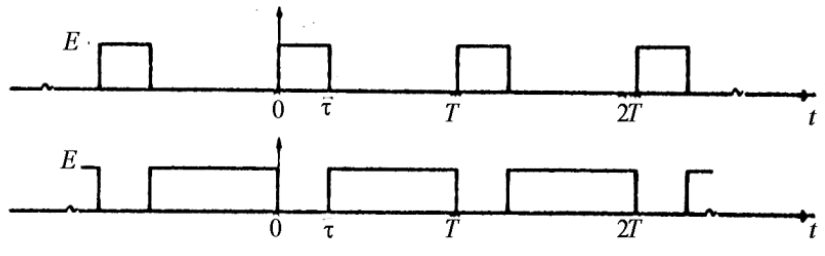
\includegraphics[width=0.6\columnwidth]{pics/fall/1/x.png}
\end{figure}

Огибающие спектров этих последовательностей:
\begin{align*}
	\widetilde{\Capit{X}}_1(\omega) &= \int \limits_{0}^{T} \s{x}_1(t)e^{-j \omega t} dt =
	E \int \limits_{0}^{\tau} e^{-j \omega t} dt = \frac{E}{-j \omega} \Big(e^{-j \omega \tau} - 1 \Big)
	=\\&= \frac{2 E}{\omega} e^{-j \frac{\omega \tau}{2}} \Bigg(\dfrac{e^{+j \frac{\omega \tau}{2}} - e^{-j \frac{\omega \tau}{2}}}{2 j} \Bigg) = ET \frac{\tau}{T} e^{-j \frac{\omega \tau}{2}} \cdot \sinc\Big(\frac{\omega \tau}{2}\Big).\\
	\widetilde{\Capit{X}}_2(\omega) &= \int \limits_{0}^{T} \s{x}_2(t)e^{-j \omega t} dt =
	E \int \limits_{\tau}^{T} e^{-j \omega t} dt 
	= \frac{E}{-j \omega} \Big(e^{-j \omega T} - e^{-j \omega \tau} \Big)
	=\\&= \frac{2 E}{\omega} e^{-\frac{j\omega}{2}(T + \tau)} \Bigg(\dfrac{e^{+\frac{j\omega}{2}(T - \tau)} - e^{-\frac{j\omega}{2}(T - \tau)}}{2 j} \Bigg) = ET \Big(1 - \frac{\tau}{T}\Big) e^{-\frac{j \omega}{2}(T + \tau)} \cdot \sinc\Big(\frac{\omega (T - \tau)}{2}\Big).
\end{align*}

\begin{figure}[!h]
	\centering
	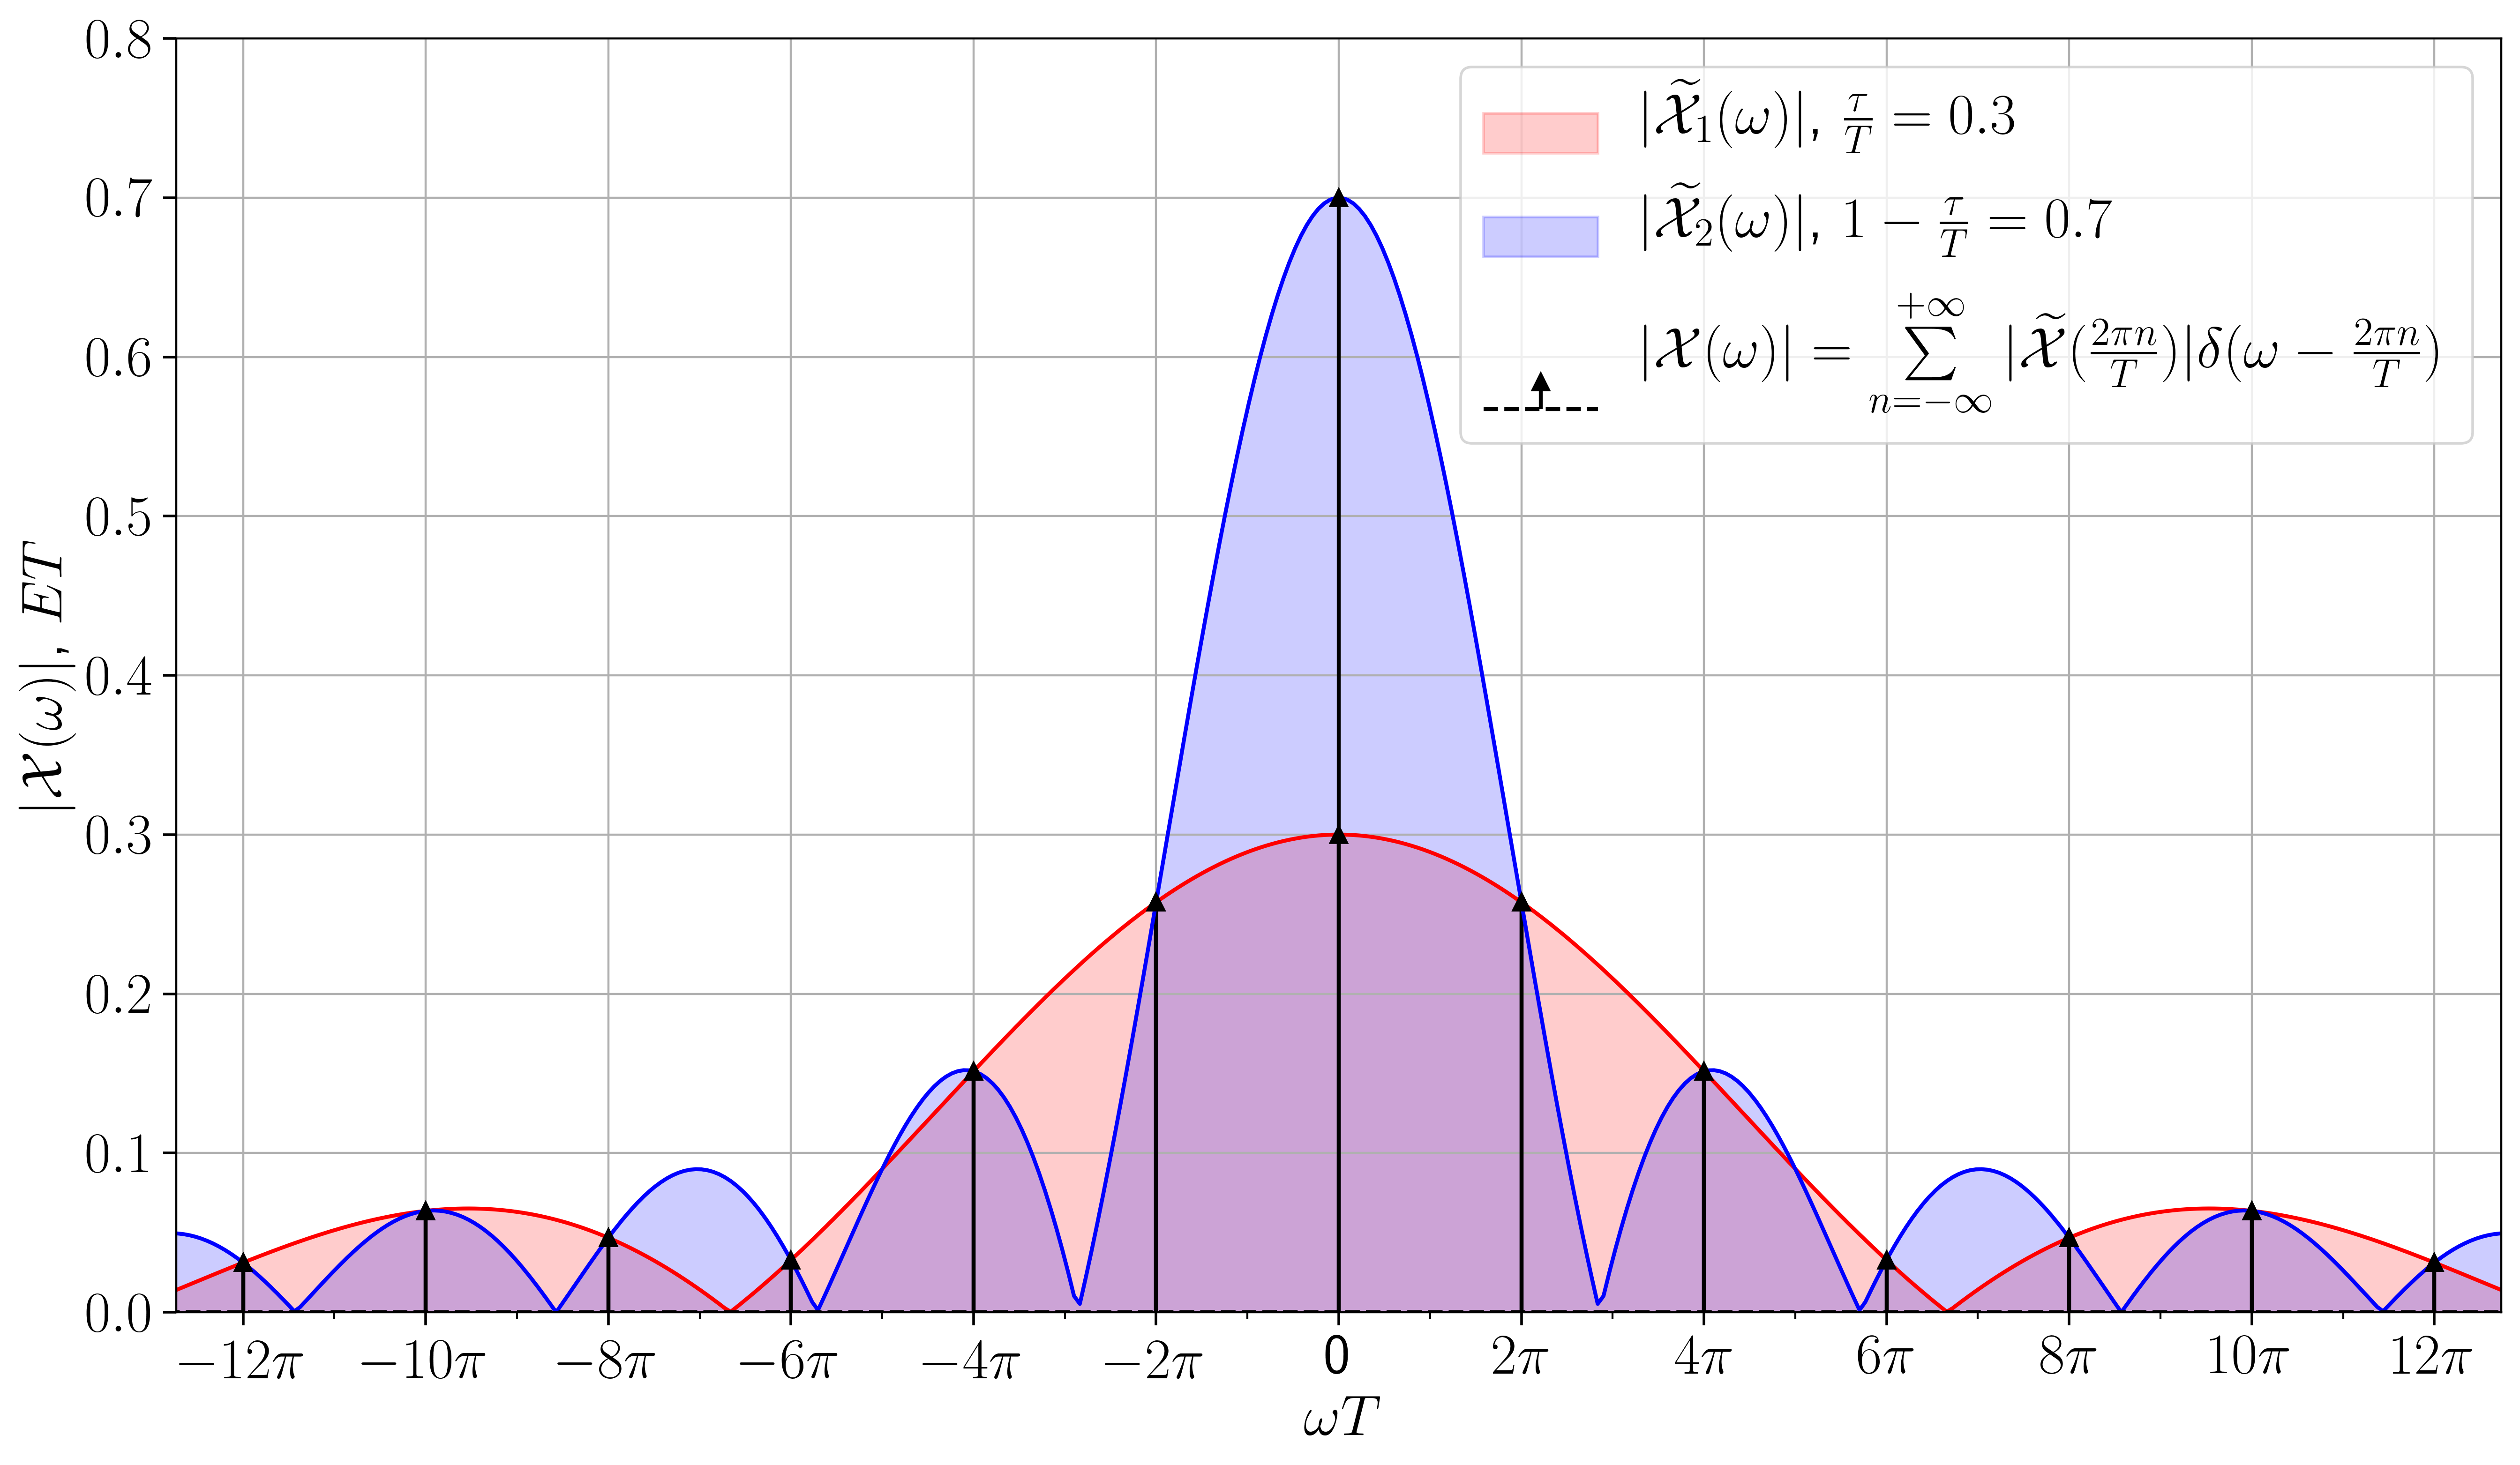
\includegraphics[width=0.95\columnwidth]{pics/fall/1/1-1.png}
	\label{fig:1}
\end{figure}

Максимальные значения спектральной плотности достигаются при $\omega = \omega_n = 0$, пропорциональны параметру скважности и соответственно равны $ET\cdot \frac{\tau}{T}$, $ET\cdot \Big( 1 - \frac{\tau}{T} \Big)$.



\section{}
Определить спектр окна Ханна длительностью $\tau = 2T$:
\begin{equation*}
	\s{w}(t) = 
	\begin{cases}
		\frac{1}{2} \Big(1 + \cos\big(\frac{\pi t}{T}\big) \Big) = \frac{1}{2} + \frac{1}{4} \Big(e^{-j\frac{\pi t}{T}} + e^{j\frac{\pi t}{T}}\Big),&\text{если } |t|< T\\
		0,&\text{если } |t|\geq T
	\end{cases}.
\end{equation*}

Найти отношение уровней первого бокового и главного лепестков.

\begin{align*}
	&\Capit{W}(\omega) = \int \limits_{-\infty}^{+\infty} \s{w}(t) e^{-\s{j} \omega t} dt = 
	\frac{1}{2} \int \limits_{-T}^{+T} e^{-\s{j} \omega t} dt + 
	\frac{1}{4} \int \limits_{-T}^{+T} e^{-\s{j} (\omega + \frac{\pi}{T}) t} dt + 
	\frac{1}{4} \int \limits_{-T}^{+T} e^{-\s{j} (\omega - \frac{\pi}{T}) t} dt =\nonumber\\
	&=\frac{1}{2} \Capit{D}_{T}(\omega) + \frac{1}{4}\Capit{D}_{T}\big(\omega + \frac{\pi}{T}\big) + \frac{1}{4}\Capit{D}_{T}\big(\omega - \frac{\pi}{T}\big) \footnotemark  =\dfrac{\sin(\omega T)}{\omega} + \frac{T}{2} \dfrac{\sin(\omega T + \pi)}{(\omega T + \pi)} + \frac{T}{2} \dfrac{\sin(\omega T - \pi)}{(\omega T - \pi)}=\\
	&=\dfrac{\sin(\omega T)}{\omega} - \frac{T}{2} \dfrac{\sin(\omega T)}{(\omega T + \pi)} - \frac{T}{2} \dfrac{\sin(\omega T)}{(\omega T - \pi)} = \dfrac{- (\pi T)^2 sin(\omega T)}{\omega T ((\omega T)^2 - \pi^2)}.
\end{align*}

\footnotetext{$\Capit{D}_T(\omega)$ -- спектр прямоугольного окна длительностью $\tau=2T$.}

\begin{align*}
	&\dfrac{d \Capit{W}(\omega)}{d\omega} = 0, \quad \Rightarrow \omega \in \{0, \pm 7.4202, \pm 10.706, \pm 13.9175, \ldots\}. \\
	&\Bigg| \dfrac{\Capit{W}(\omega_1)}{\Capit{W}(\omega_0)} \Bigg|^2 = \Big| \Capit{W}(7.4202) \Big|^2 = 0.02671^2 = 0.0007133 = -31.47\text{ dB}.
\end{align*}


\begin{figure}[!h]
	\centering
	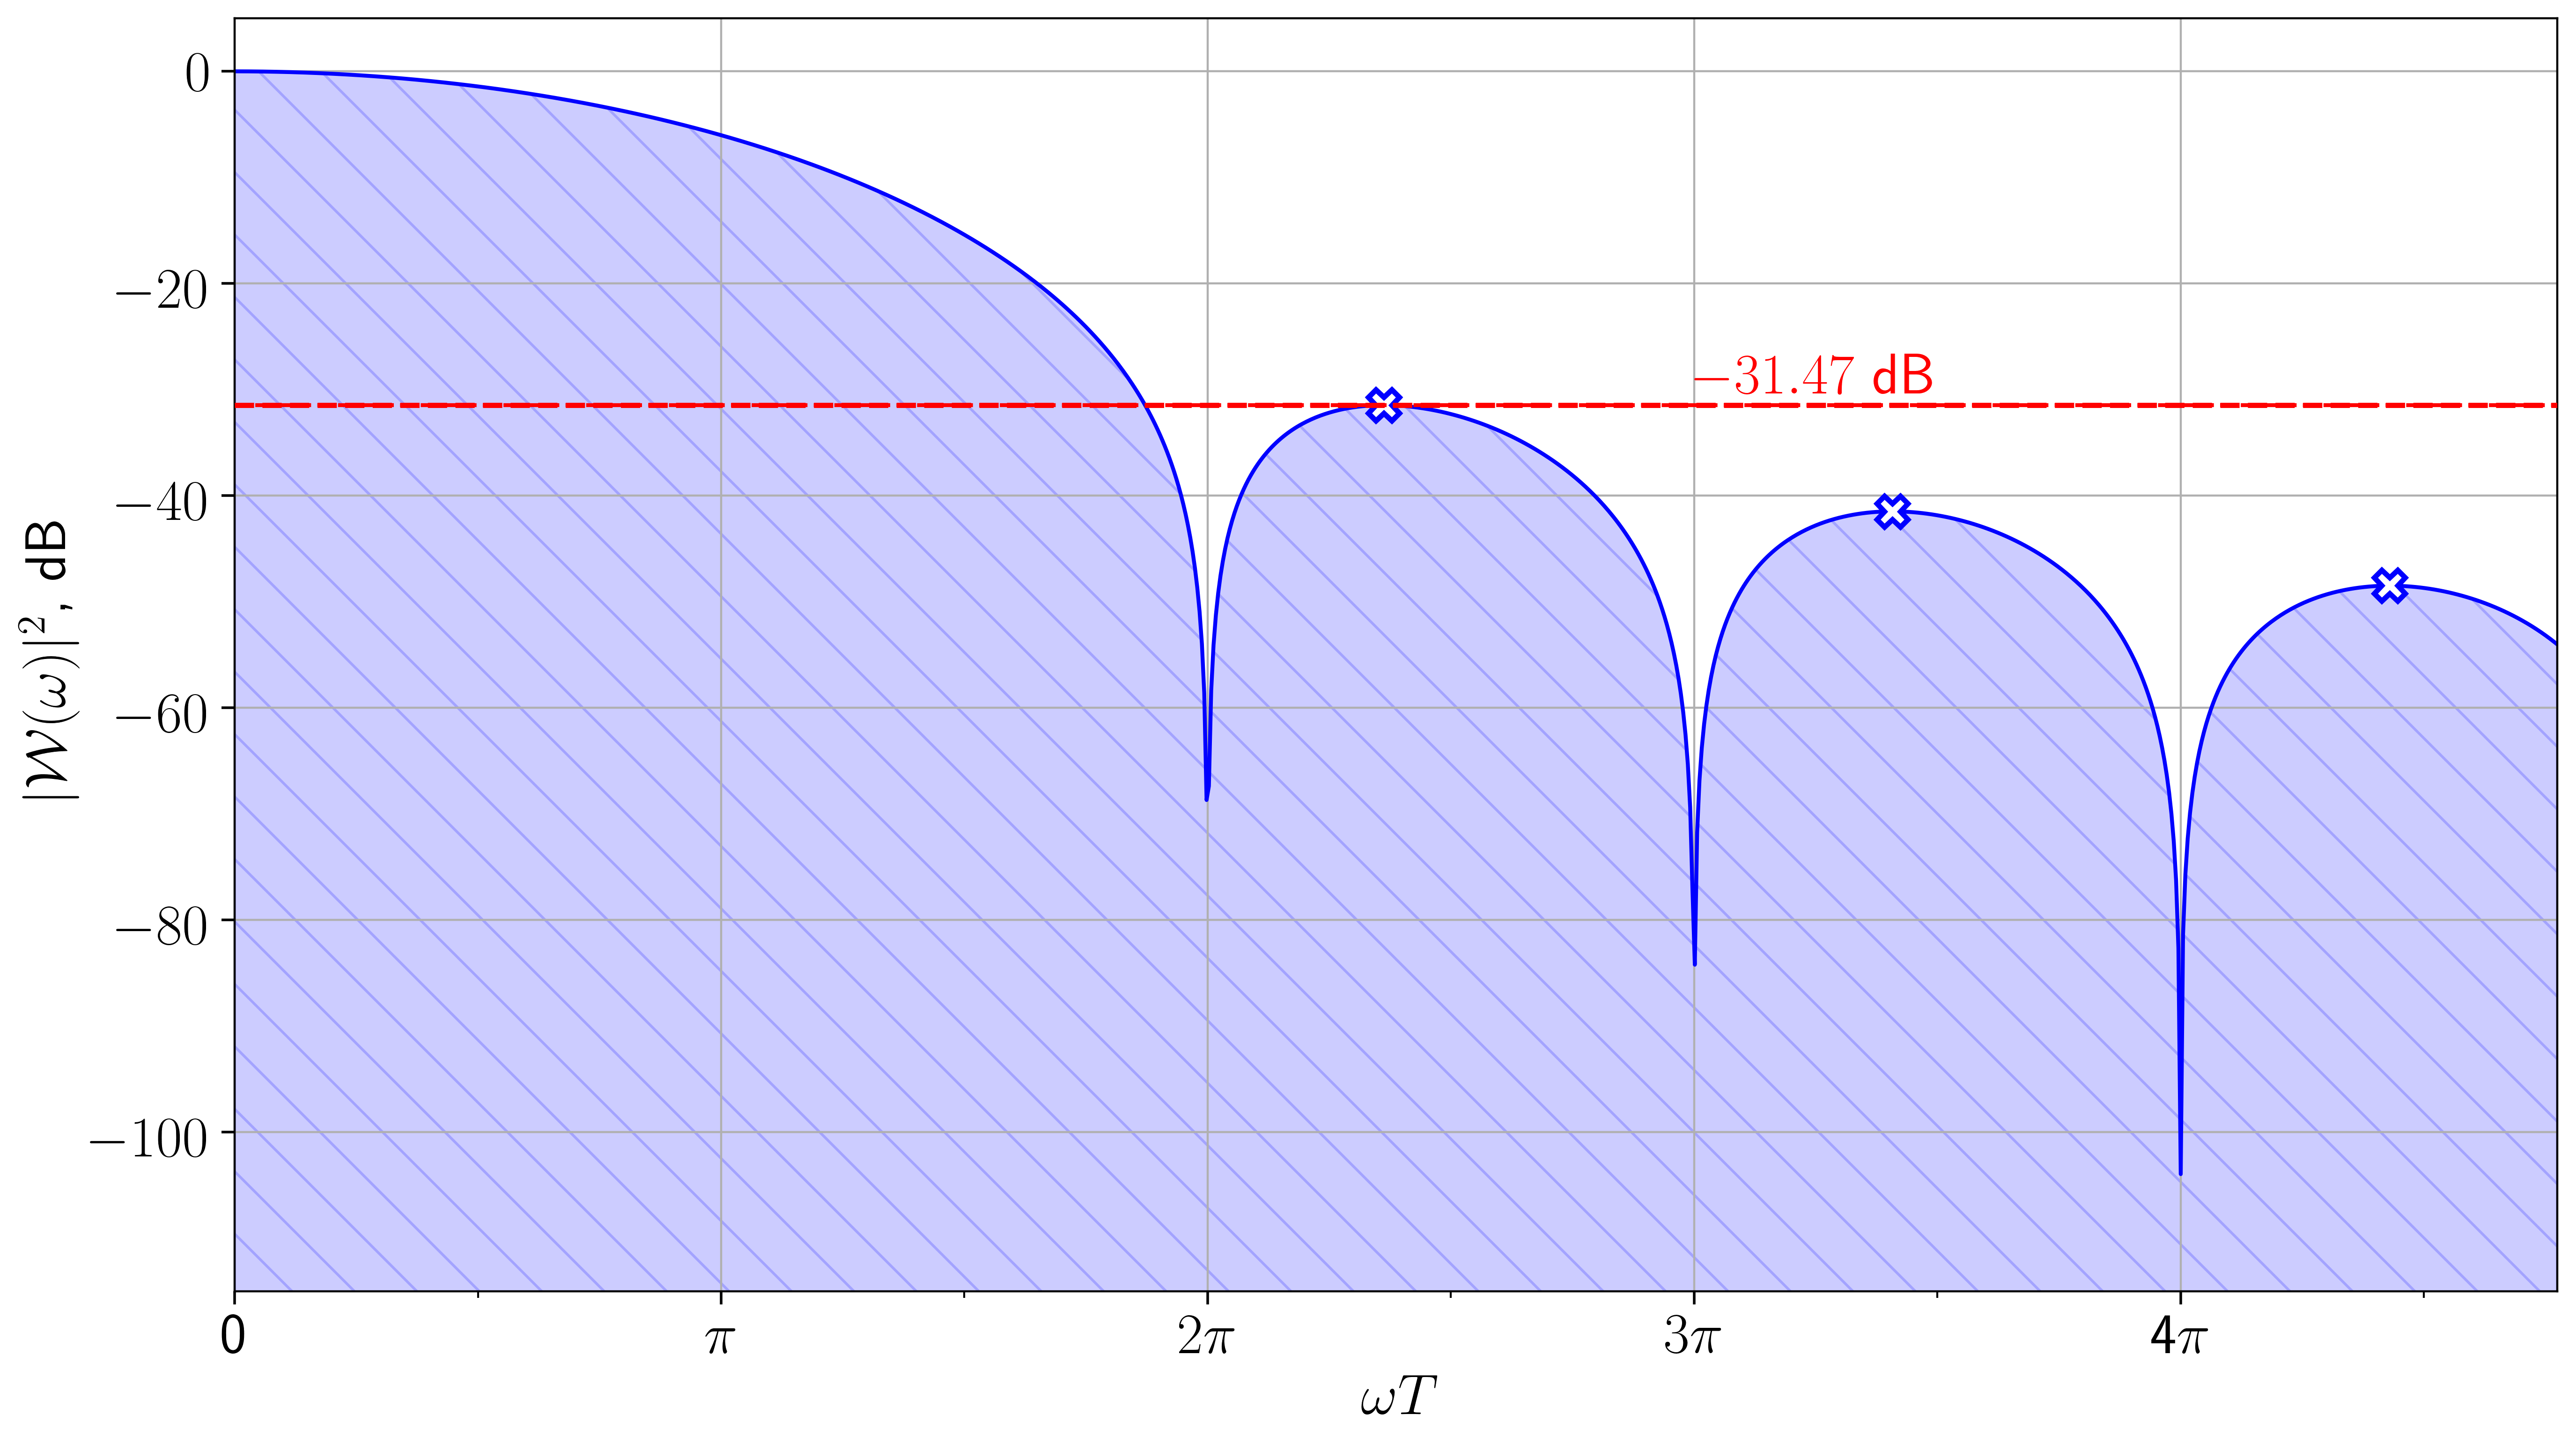
\includegraphics[width=0.95\columnwidth]{pics/fall/1/1-2.png}
	\caption{Спектр окна Ханна.}
	\label{fig:topology}
\end{figure}


\section{}
Найти спектр функции отсчетов, используемых в теореме Котельникова.

\begin{equation*}
	\phi_k(t) = \dfrac{\sin(2\pi f_B(t - k \Delta t))}{2\pi f_B(t - k \Delta t)},\quad \Delta t = \dfrac{1}{2f_{B}}.
\end{equation*}


Доказать их ортогональность, используя равенство Парсеваля для прямоугольного импульса и дуализм времени и частоты преобразовании Фурье.

\begin{align*}
	&\Phi_k(f) = \int \limits_{-\infty}^{+\infty} \phi_k (t) e^{-j 2\pi f t} dt = \int \limits_{-\infty}^{+\infty} \dfrac{\sin(2\pi f_B(t - k \Delta t))}{2\pi f_B(t - k \Delta t)} e^{-j 2\pi f t} dt = 
	\dfrac{e^{j 2\pi f k \Delta t}}{2\pi f_B}\int \limits_{\infty}^{+\infty} \textcolor{blue}{\dfrac{\sin(\s{u})}{\s{u}}} e^{-j \s{u} \frac{f}{f_B}} d\s{u} =\\
	&= \dfrac{e^{j 2\pi f k \Delta t}}{2\pi f_B}\int \limits_{\infty}^{+\infty} \textcolor{blue}{\Big(\int \limits_{-1}^{+1} \frac{1}{2} e^{j \s{uv}} d \s{v} \Big)} e^{-j \s{u} \frac{f}{f_B}} d\s{u} = 
	\frac{1}{2}  \dfrac{e^{j 2\pi f k \Delta t}}{2\pi f_B} \int \limits_{-1}^{+1} d \s{v} \textcolor{red}{\int \limits_{-\infty}^{\infty} e^{j (\s{v} - \frac{f}{f_B}) \s{u}} d \s{u}} = 
	\frac{1}{2}  \dfrac{e^{j 2\pi f k \Delta t}}{2\pi f_B} \int \limits_{-1}^{+1} d \s{v} \cdot \textcolor{red}{2 \pi \delta \Big(\s{v} - \frac{f}{f_B}\Big)} =\\
	&= \pi \dfrac{e^{j 2\pi f k \Delta t}}{2\pi f_B} \Bigg[\Theta \Big(1 - \frac{f}{f_B} \Big) - \Theta \Big(- 1 - \frac{f}{f_B} \Big) \Bigg] = 
	\pi \dfrac{e^{j 2\pi f k \Delta t}}{2\pi f_B} \Bigg[\Theta \Big( f + f_{B}\Big) - \Theta \Big(f - f_B\Big) \Bigg].
\end{align*}

Согласно равенству Парсеваля:
\begin{align*}
	\braket{\phi_k|\phi_n} &= \int \limits_{-\infty}^{+\infty} \phi_k(t)\phi_n(t)dt 
	= \int \limits_{-\infty}^{+\infty} \Phi_k(f) \Phi_n^*(f) df = 
	\dfrac{\pi^2}{(2 \pi  f_B)^2} \int \limits_{-f_B}^{f_B} e^{j2\pi f (k - n) \Delta t} df = \\
	&= \dfrac{\pi^2}{(2 \pi  f_B)^2} \dfrac{e^{j2\pi f_B (k - n) \Delta t} - e^{-j2\pi f_B (k - n) \Delta t}}{j2 \pi (k - n) \Delta t} = 
	\dfrac{\pi^2}{(2 \pi  f_B)^2} \dfrac{\sin(2\pi f_B (k - n) \Delta t)}{\pi (k - n) \Delta t} = 
	\dfrac{\sin(\pi (k - n))}{2 \pi  f_B (k - n)} = 0.\\
	\braket{\phi_k|\phi_k} &= \dfrac{\pi^2}{(2 \pi  f_B)^2} \int \limits_{-f_B}^{f_B} e^{j2\pi f (k - k) \Delta t} df =
	\dfrac{1}{2 f_B} = \Delta t.
\end{align*}

\begin{equation*}
	\boxed{\braket{\phi_k|\phi_n} = \delta_{kn} \Delta t. }
\end{equation*}



\setcounter{chapter}{2}
\setcounter{section}{0}
%\chapter*{Неделя 2}
\protect\thispagestyle{fancy}
\section{}
Гармонический сигнал $x(t) = \cos(2 \pi f_0 t)$, $f_0 = 500$ кГц дискретизован с частотой $f_{d} = 2$ МГц. Изобразить как функцию нормированной частоты $\nu = f/f_{d}$ в диапазоне $|\nu|\leq2$ 
\begin{itemize}
	\item модуль спектра исходного сигнала;
	\item модуль спектра дискретизованного сигнала;
	\item модуль спектра последовательности $z(k) = x(k)\cdot 2\cos(k \pi /2)$.
\end{itemize}


\begin{align*}
	&x(t) = \dfrac{1}{2}e^{j 2 \pi f_d \nu_0 t} + \dfrac{1}{2}e^{-j 2 \pi f_d \nu_0 t},\quad \text{где }\nu_0 = \frac{f_0}{f_d} = \frac{0.5}{2} = \frac{1}{4}.\\
	&z(k) = \dfrac{1}{2}\Big(e^{j 2 \pi \nu_0 k} + e^{-j 2 \pi \nu_0 k}\Big)
	\Big(e^{j \frac{\pi k}{2}} + e^{-j \frac{\pi k}{2}}\Big) =  
	\dfrac{1}{2}\Big(e^{j 2 \pi \frac{1}{2} k} + 2e^{0} + e^{-j 2 \pi \frac{1}{2} k} \Big).
\end{align*}

Спектр исходного и дискретизованного сигналов:\footnote[1]{Часто нормировка весов дельта-функций на $\frac{1}{f_d}$ подразумевается автоматически и может быть опущена.}
\begin{align*}
	&\Capit{X}(f) = \dfrac{1}{2}(\delta(f-f_0)+\delta(f+f_0))
	\quad \Leftrightarrow \quad
	\Capit{X}(\nu) = \dfrac{1}{2f_d}(\delta(\nu-\nu_0) + \delta(\nu+\nu_0)).\\
	&\Capit{X}_d(f) = \dfrac{1}{2}\sum\limits_{m=-\infty}^{+\infty}(\delta(f-f_0-mf_d)+\delta(f+f_0-mf_d)) \quad \Leftrightarrow \quad
	\Capit{X}_d(\nu) = \dfrac{1}{2f_d}\sum\limits_{m=-\infty}^{+\infty}(\delta(\nu-\nu_0-m)+\delta(\nu+\nu_0-m)).
\end{align*}

Спектры последовательности $z(k)$:
\begin{align*}
	&\Capit{Z}(\nu) = \dfrac{1}{2f_d}\Bigg[\delta\Big(\nu+\frac{1}{2}\Big) + 2\delta(\nu) + \delta\Big(\nu-\frac{1}{2}\Big)\Bigg].\\
	&\Capit{Z}_{d}(\nu) = \dfrac{1}{2f_d}\sum\limits_{m=-\infty}^{+\infty}\Bigg[\delta\Big(\nu+\frac{1}{2}-m\Big) +2\delta(\nu-m) + \delta\Big(\nu-\frac{1}{2}-m\Big)\Bigg] =
	\dfrac{1}{f_d}\sum\limits_{m=-\infty}^{+\infty} \Bigg[\delta\Big(\nu-\frac{1}{2}-m\Big) +\delta(\nu-m)\Big)\Bigg].
\end{align*}

\begin{figure}[!h]
	\centering
	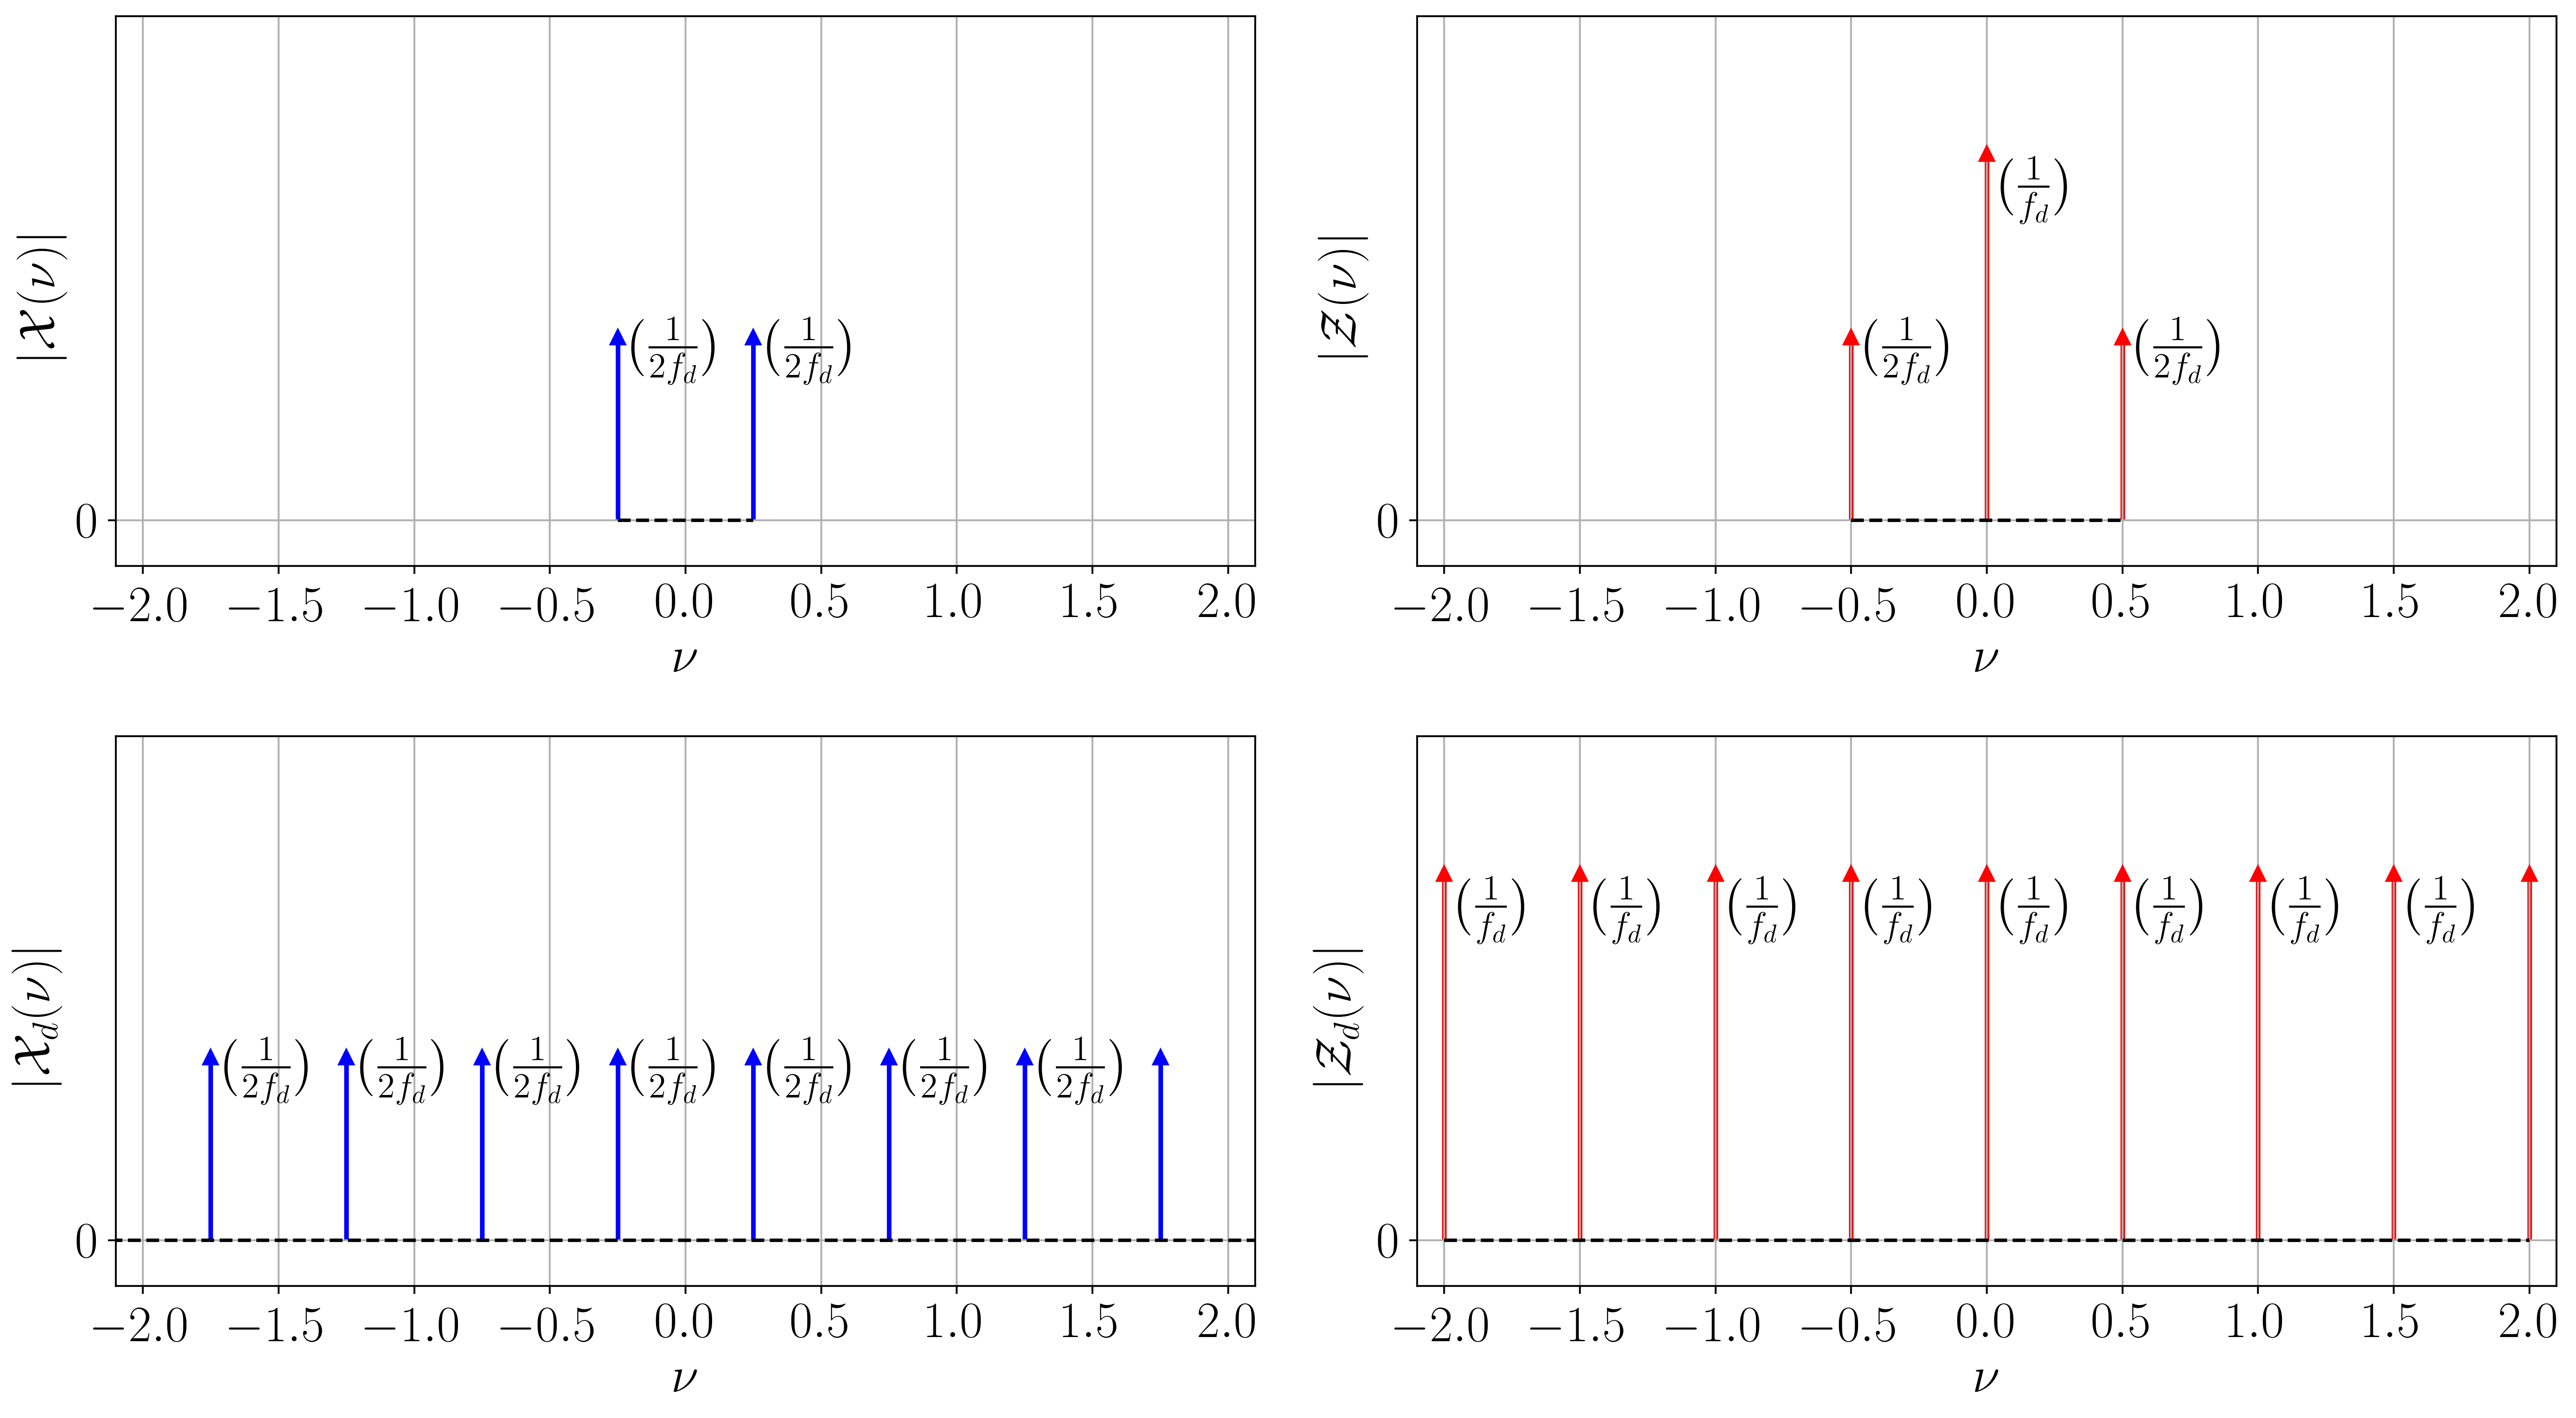
\includegraphics[width=0.90\columnwidth]{pics/fall/2/2-1.png}
	\label{fig:2-1}
\end{figure}


\newpage
\section{}
Сигнал $x(t)$ имеет финитный спектр треугольного вида. Определить коэффициенты ряда Котельникова этого сигнала, полагая, что $\Delta t = \dfrac{1}{2f_{b}}$.

\begin{figure}[!h]
	\centering
	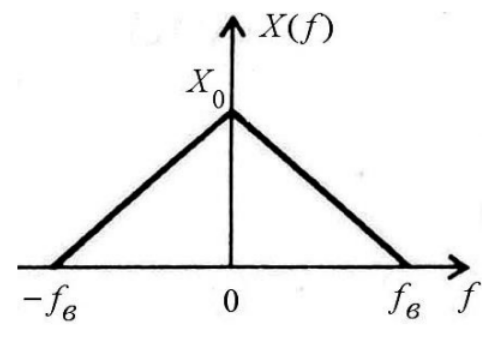
\includegraphics[width=0.20\columnwidth]{pics/fall/2/triangle.png}
	\label{2_triangle}
\end{figure}


\begin{align*}
	c_k &= \dfrac{\braket{x|\phi_k}}{\braket{\phi_k|\phi_k}} = \dfrac{1}{\Delta t} \int\limits_{-\infty}^{+\infty}x(t)\dfrac{\sin(2\pi f_b(t - k \Delta t))}{2\pi f_b(t - k \Delta t)}dt =
	\dfrac{1}{\Delta t} \int\limits_{-\infty}^{+\infty}\Capit{X}(f)\Phi_k(f)df = \int\limits_{-\infty}^{+\infty}\Capit{X}(f) e^{j 2\pi f k \Delta t} \Theta \big(-f_b \leq  f \leq f_{b}\big) df =\\
	&=\int\limits_{-f_b}^{+f_b}\Capit{X}(f) e^{j 2\pi f k \Delta t}df = \dfrac{\Capit{X}_0}{f_b}\Bigg\{\int\limits_{-f_b}^{0} (f_b + f) e^{j 2\pi f k \Delta t}df + \int\limits_{0}^{f_b} (f_b - f) e^{j 2\pi f k \Delta t}df\Bigg\} =\\
	&=\dfrac{\Capit{X}_0}{j2\pi k f_b \Delta t}\Bigg\{(f_b + f)e^{j 2\pi f k \Delta t}\Bigg|_{-f_b}^0 + (f_b - f)e^{j 2\pi f k \Delta t}\Bigg|_{0}^{f_b}
	- \int\limits_{-f_b}^{0} e^{j 2\pi f k \Delta t}df + \int\limits_{0}^{f_b} e^{j 2\pi f k \Delta t}df\Bigg\} = \\
	&=\dfrac{\Capit{X}_0}{j\pi k}\Bigg\{f_b - f_b + \dfrac{1}{j 2\pi k \Delta t} \Bigg(e^{j 2\pi f k \Delta t}\Bigg|_{0}^{f_b} - e^{j 2\pi f k \Delta t}\Bigg|_{-f_b}^{0} \Bigg) \Bigg\} =
	\dfrac{\Capit{X}_0}{(j\pi k)^2 2\Delta t}\Bigg\{-2 + e^{j 2\pi f_b k \Delta t} + e^{-j 2\pi f_b k \Delta t} \Bigg \} = \\
	&= \dfrac{\Capit{X}_0}{(\pi k)^2 \Delta t} - \dfrac{\Capit{X}_0}{(\pi k)^2 \Delta t}\cos(2\pi f_b k \Delta t) = \dfrac{\Capit{X}_0}{(\pi k)^2 \Delta t} - \dfrac{\Capit{X}_0}{(\pi k)^2 \Delta t}\cos(\pi k) = \dfrac{2\Capit{X}_0}{(\pi k)^2 \Delta t}\sin^2 \Big(\frac{\pi k}{2}\Big) = \dfrac{4 \Capit{X}_0 f_b}{(\pi k)^2}\sin^2 \Big(\frac{\pi k}{2}\Big).
\end{align*}

\section{}
Найти и изобразить по модулю ДВПФ $16$-точечных последовательностей:
\begin{equation*}
	x(k) = \sum \limits_{m=0}^{15}\mathbf{1}(k-m) \quad \text{и}\quad y(k) = x(k)z(k),\text{ где }z(k) = \cos\Big(2 \pi k \frac{3}{16}\Big).
\end{equation*}

\begin{align*}
	&\Capit{X}_{N}(\nu) = \sum \limits_{k = 0}^{N-1} x(k)e^{-j2\pi \nu k} = \sum \limits_{k = 0}^{N-1} e^{-j2\pi \nu k} = 
	\dfrac{1 - e^{-j 2 \pi \nu N}}{1 - e^{-j 2 \pi \nu}} = \dfrac{e^{-j \pi \nu N}}{e^{-j \pi \nu}} 
	\dfrac{e^{j \pi \nu N} - e^{-j \pi \nu N}}{e^{j \pi \nu} - e^{-j \pi \nu}} = e^{-j \pi \nu (N-1)}\dfrac{\sin(N \pi \nu)}{\sin(\pi \nu)}.\\
	&\Capit{Z}(\nu) = \sum \limits_{k = -\infty}^{+\infty} z(k)e^{-j2\pi \nu k} = \dfrac{1}{2}\sum \limits_{k=-\infty}^{+\infty} e^{-j2\pi \big(\nu - \frac{3}{16}\big) k} + \dfrac{1}{2}\sum \limits_{k =-\infty}^{+\infty} e^{-j2\pi \big(\nu + \frac{3}{16}\big) k} = \dfrac{1}{2}\sum \limits_{m = -\infty}^{+\infty}\Big[\delta\big(\nu - \frac{3}{16}-m\big) + \delta\big(\nu + \frac{3}{16}-m\big)\Big].\\
	&\Capit{Y}(\nu) = \int \limits_{-\frac{1}{2}}^{\frac{1}{2}}\Capit{X}_{16}(\tilde{\nu})\Capit{Z}(\nu - \tilde{\nu})d\tilde{\nu} = \dfrac{1}{2}\int \limits_{-\frac{1}{2}}^{\frac{1}{2}}\Capit{X}_{16}(\tilde{\nu})\sum \limits_{m = -\infty}^{+\infty}\Big[\delta\big(\nu - \tilde{\nu} - \frac{3}{16}-m\big) + \delta\big(\nu - \tilde{\nu} + \frac{3}{16}-m\big)\Big]d \tilde{\nu} =\\
	&=\dfrac{1}{2}\Capit{X}_{16} \big(\nu - \frac{3}{16}\big) + \dfrac{1}{2}\Capit{X}_{16} \big(\nu + \frac{3}{16}\big) = e^{-j \pi 15(\nu - \frac{3}{16})}\dfrac{\sin(16 \pi (\nu - \frac{3}{16}))}{2\sin(\pi (\nu - \frac{3}{16}))} + 
	e^{-j \pi 15(\nu + \frac{3}{16})}\dfrac{\sin(16 \pi (\nu + \frac{3}{16}))}{2\sin(\pi (\nu + \frac{3}{16}))}.
\end{align*}


\begin{figure}[!h]
	\centering
	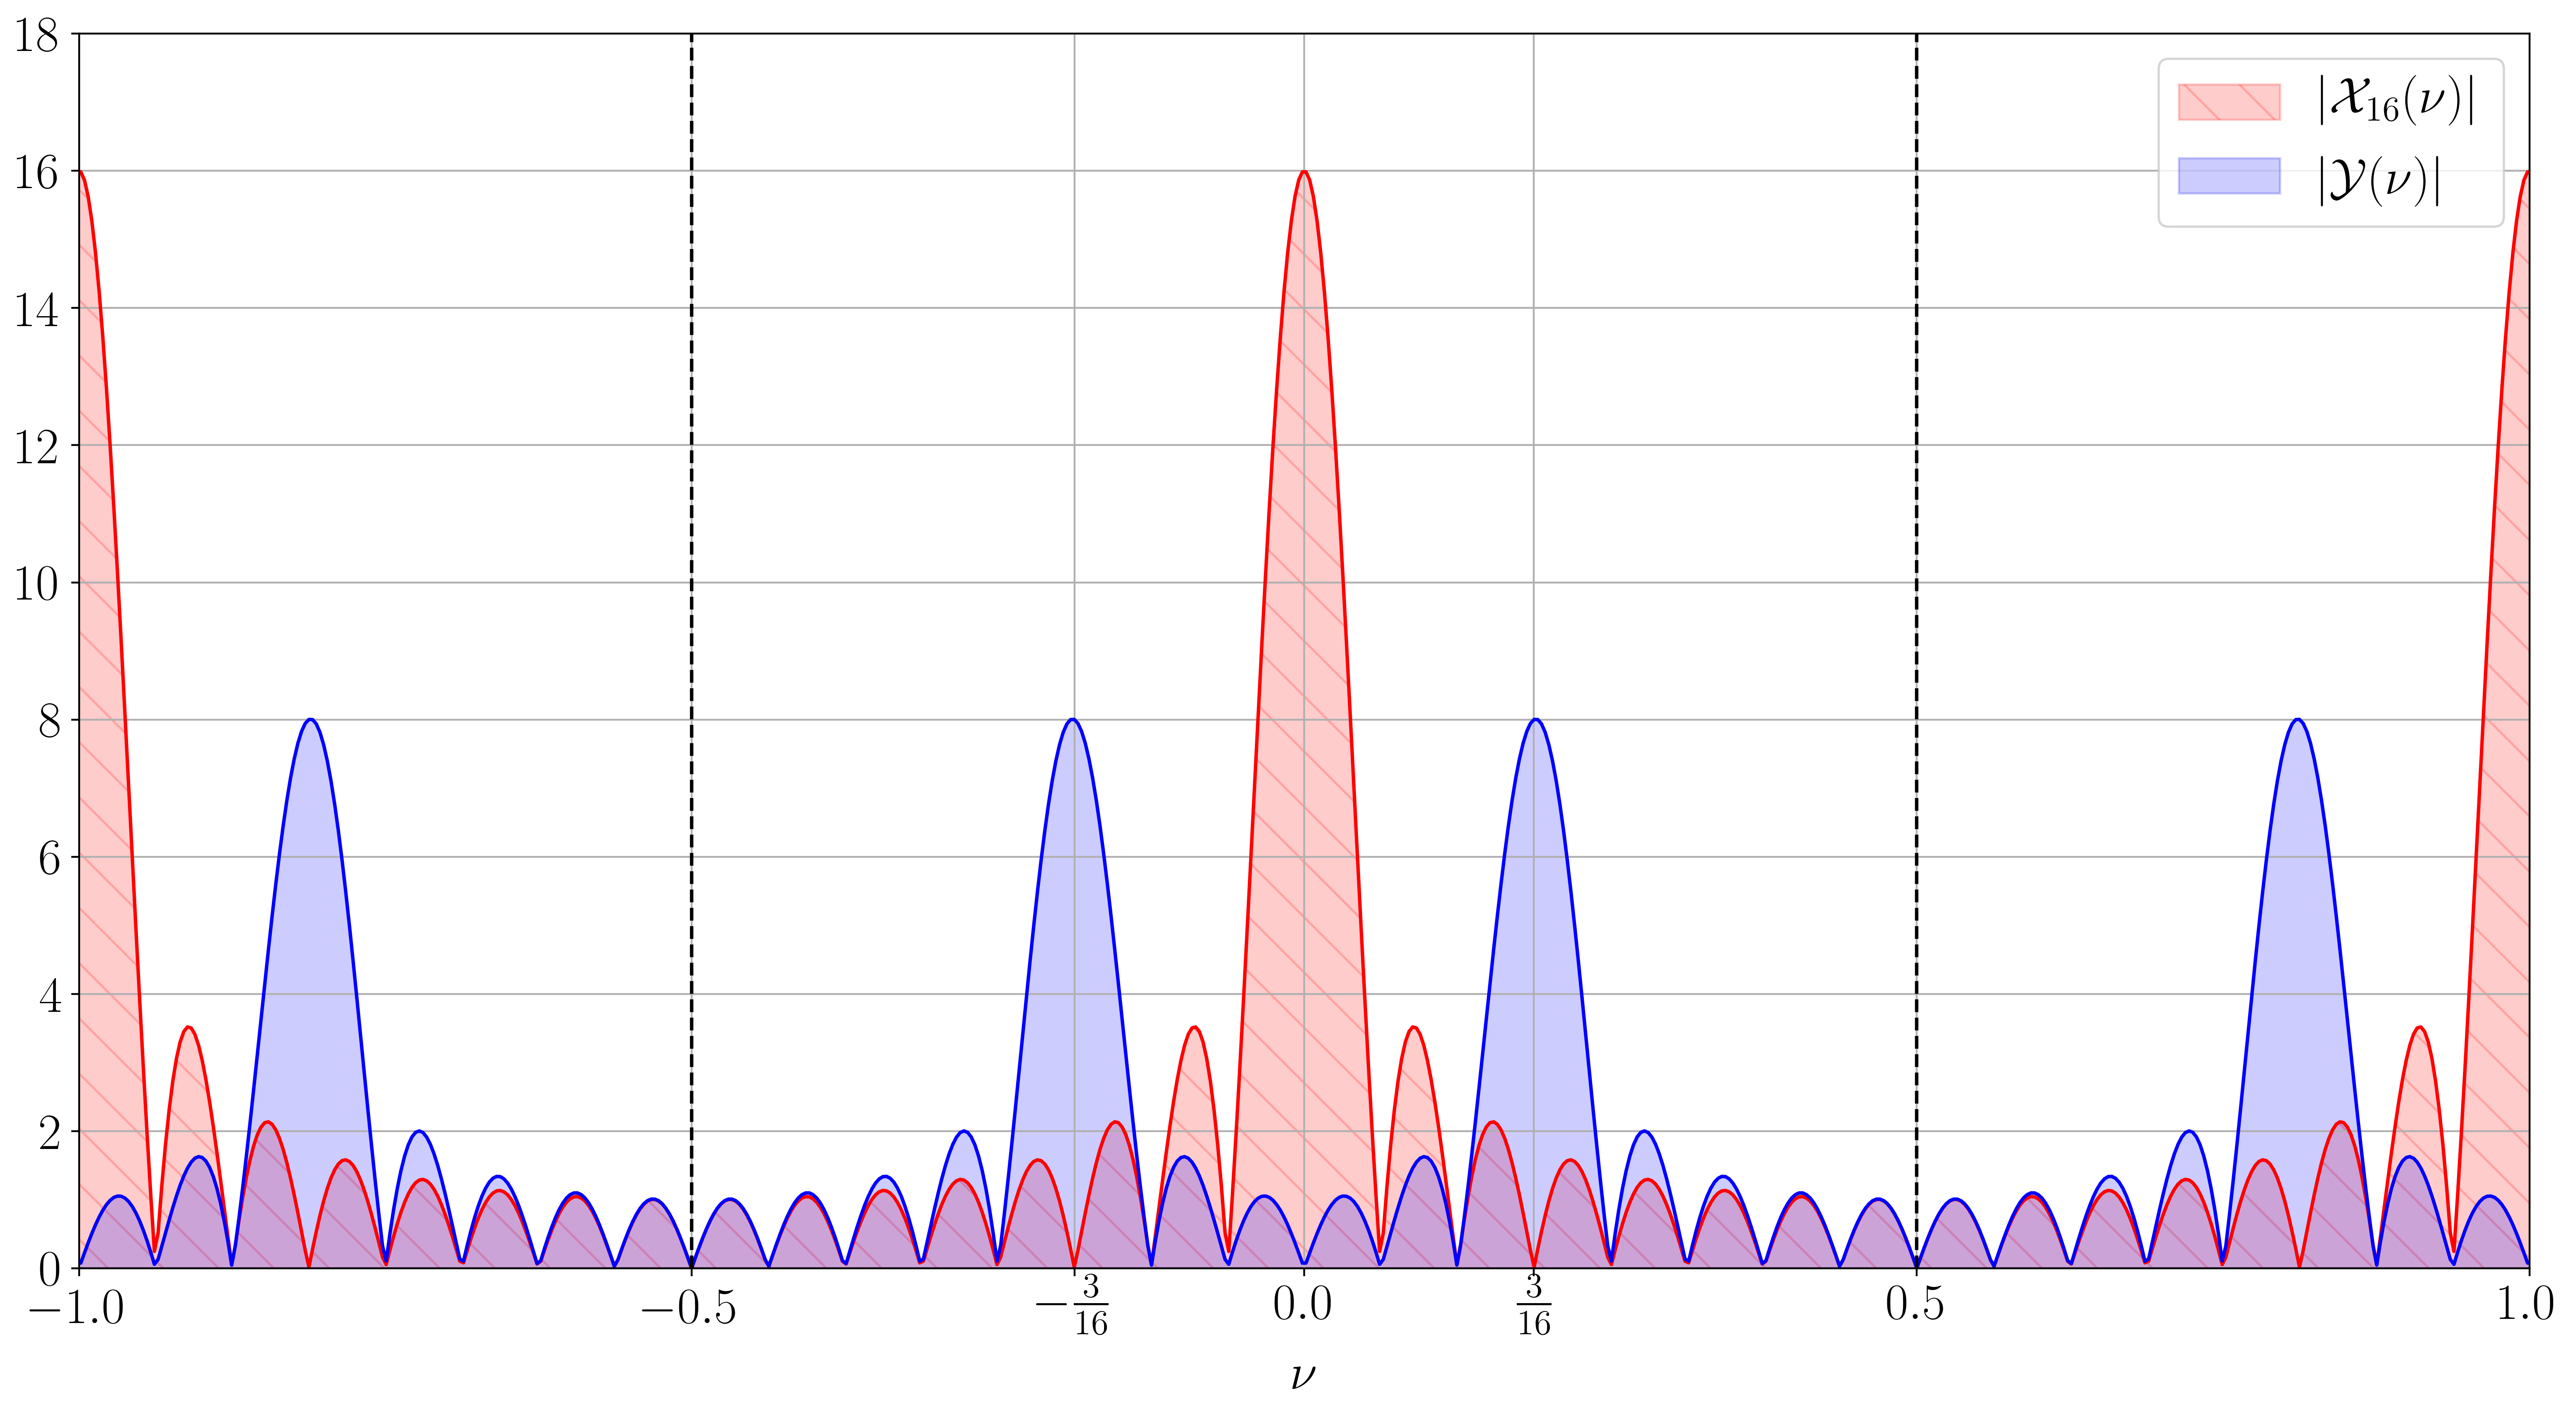
\includegraphics[width=1.0\columnwidth]{pics/fall/2/2-3.png}
	\label{fig:2-3}
\end{figure}


\section{}
Сформулировать и доказать теорему о свёртке последовательностей для ДВПФ.

\textit{Теорема:}

Пусть $\Capit{X}(\nu) = \sum\limits_{k = -\infty}^{+\infty}x(k)e^{-j 2 \pi \nu k}$ и $\Capit{Y}(\nu) = \sum\limits_{k = -\infty}^{+\infty}y(k)e^{-j 2 \pi \nu k}$, тогда дискретной свёртке двух сигналов $z(k) = \sum \limits_{m = -\infty}^{+\infty} x(m)y(k-m)$ отвечает произведение их спектров $\Capit{Z}(\nu) = \Capit{X}(\nu)\Capit{Y}(\nu)$.

\textit{Доказательство:}
\begin{align*}
	\Capit{Z}(\nu) &= \sum\limits_{k = -\infty}^{+\infty}z(k)e^{-j 2 \pi \nu k} = \sum\limits_{k = -\infty}^{+\infty} \sum\limits_{m = -\infty}^{+\infty} x(m)y(k-m) e^{-j 2 \pi \nu m} e^{-j 2 \pi \nu (k - m)}  = \\
	&= \sum\limits_{m = -\infty}^{+\infty} x(m) e^{-j 2 \pi \nu m} \sum\limits_{n = -\infty}^{+\infty} y(n) e^{-j 2 \pi \nu n} = \sum\limits_{m = -\infty}^{+\infty} x(m) e^{-j 2 \pi \nu m} \Capit{Y}(\nu) = \Capit{X}(\nu) \Capit{Y}(\nu).
\end{align*}


\setcounter{chapter}{3}
\setcounter{section}{0}
%\chapter*{Неделя 3}
\protect\thispagestyle{fancy}
\section{}
Гармонический сигнал $x(t) = \cos(2 \pi f_0 t)$, $f_0 = 35$ Гц, дискретизован с частотой дискретизации $f_d = 140$ Гц. Найти и изобразить по модулю ДПФ и ДВПФ отрезка сигнала из восьми отсчётов.

\begin{align*}
	&x(t) =  \cos(2 \pi f_0 t) = \dfrac{1}{2}e^{j2\pi f_0 t} + \dfrac{1}{2}e^{-j2\pi f_0 t},\\
	&\Capit{X}(\nu) = \dfrac{1}{2}\sum\limits_{m = -\infty}^{+\infty}\Big[\delta(\nu - \nu_0 -m) + \delta(\nu + \nu_0 - m)\Big],\ \text{где}\ \nu_0 = \dfrac{f_0}{f_d} = \dfrac{35}{140} = \dfrac{1}{4}.\\
	&\Capit{X}_{8}(\nu) = \Capit{X}(\nu) \otimes \Capit{D}_{8}(\nu)\footnotemark  = \dfrac{1}{2} \Big[\Capit{D}_{8}(\nu - \nu_0) + \Capit{D}_{8}(\nu + \nu_0) \Big]
	= \dfrac{1}{2} \Big[e^{-j7\pi (\nu - \nu_0)}\dfrac{\sin(8\pi(\nu - \nu_0))}{\sin(\pi(\nu - \nu_0))} + e^{-j7\pi (\nu + \nu_0)}\dfrac{\sin(8\pi(\nu + \nu_0))}{\sin(\pi(\nu + \nu_0))} \Big].\\
	&\Capit{X}_{8}[n] = \sum\limits_{k=0}^{7} \cos(2 \pi \nu_0 k) e^{-j 2\pi \frac{n}{8}k} = 
	\dfrac{1}{2} \sum\limits_{k=0}^{7} \Big[e^{j 2\pi k (2 - n)/8} + e^{-j 2\pi k (2 + n)/8} \Big] =
	\begin{cases}
		4,\quad \text{если} \ n\%8 \in \{2, 6\},\\
		0,\quad \text{если} \ n\%8 \not\in \{2, 6\}.
	\end{cases}
\end{align*}
\footnotetext{$\Capit{D}_8(\nu)$ -- ДВПФ прямоугольного окна длительностью $8$.}

\begin{figure}[!h]
	\centering
	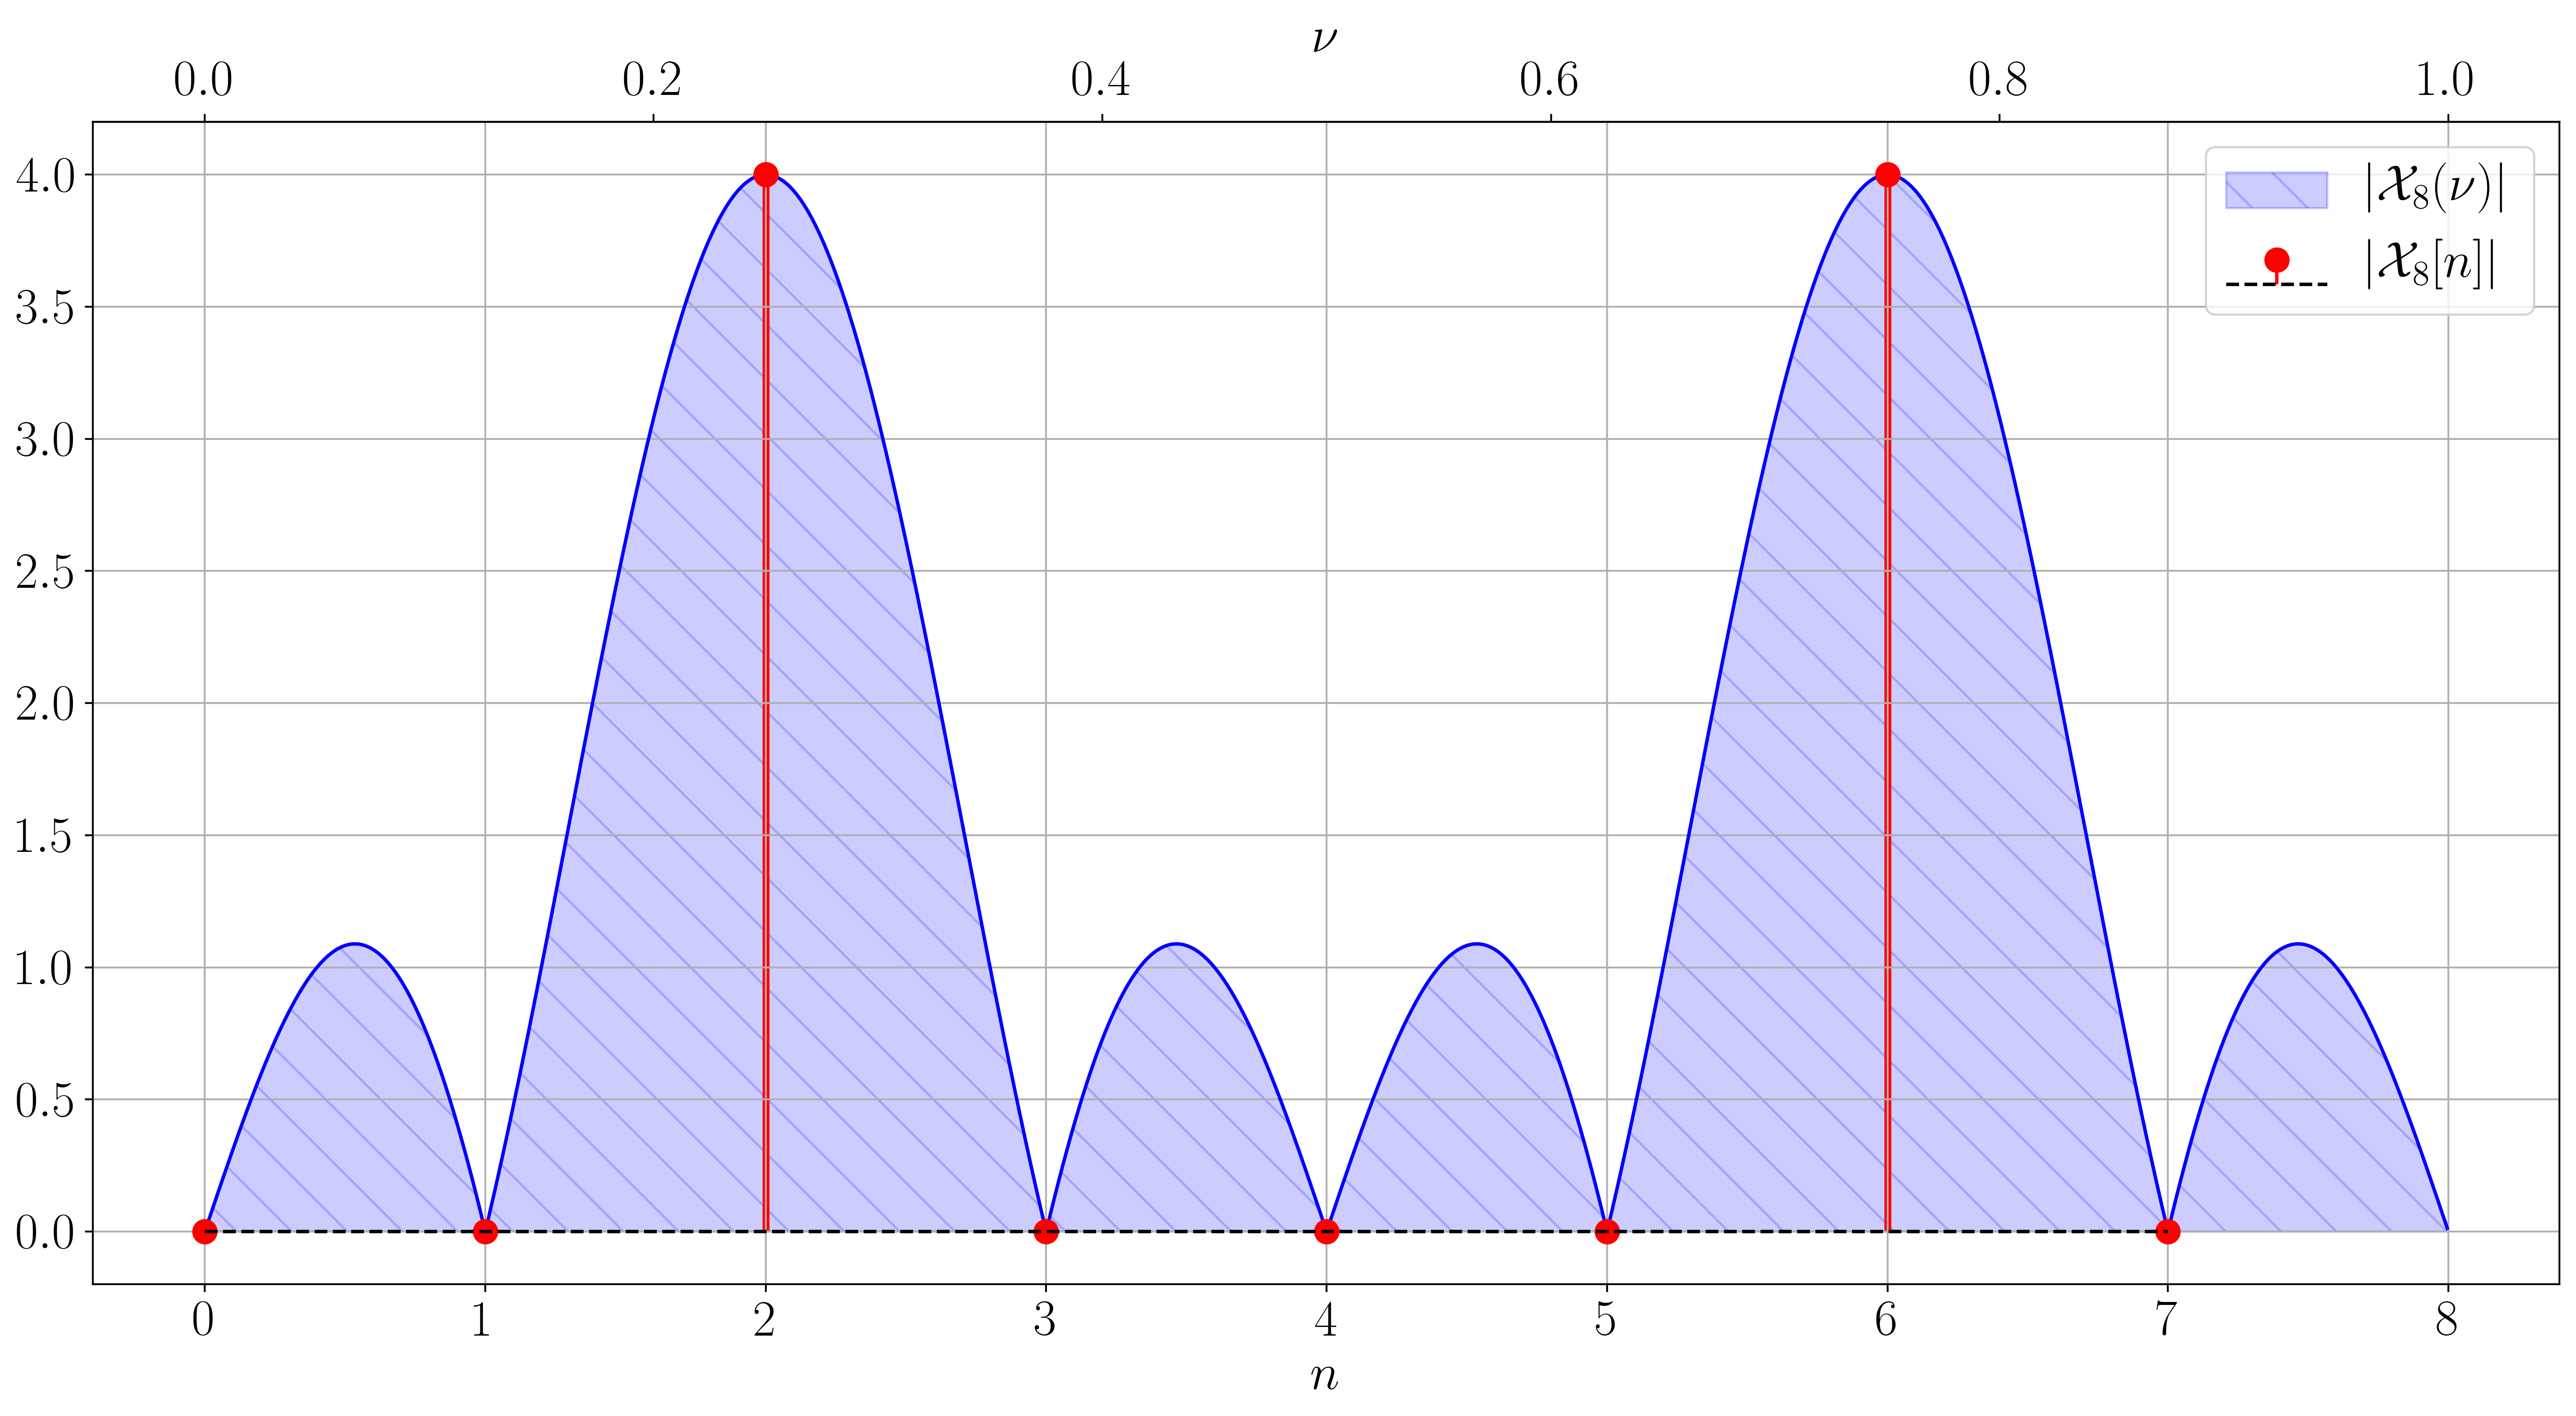
\includegraphics[width=1.0\columnwidth]{pics/fall/3/3-1.png}
	\label{fig:3-1}
\end{figure}

\newpage
\section{}

\begin{figure}[!h]
	\centering
	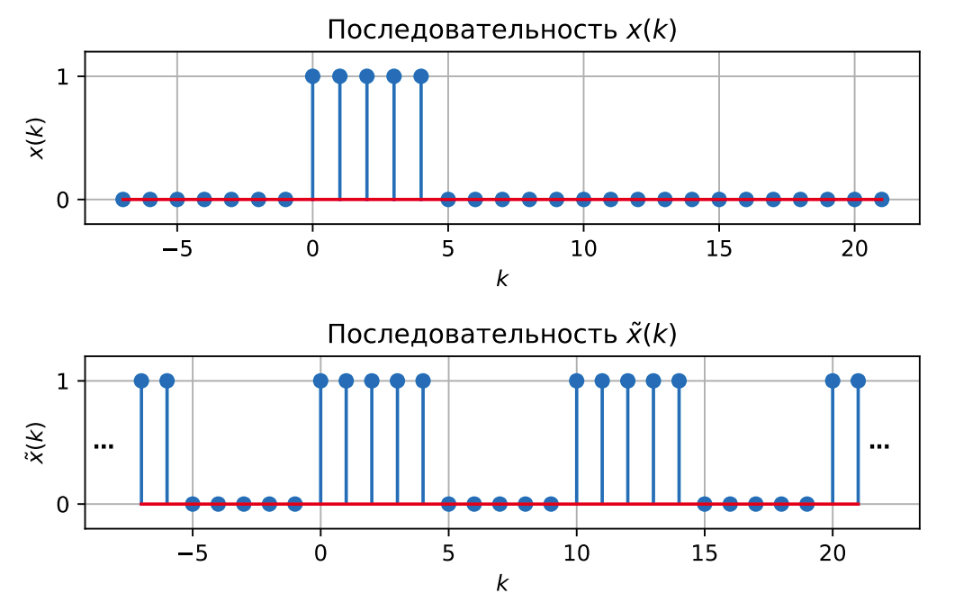
\includegraphics[width=0.5\columnwidth]{pics/fall/3/3-2-0.png}
	\label{fig:3-2-0}
\end{figure}


Изобразить модули коэффициентов ДПФ $5$-точечной последовательности $x[k]$ (пятиточечного) и её периодического продолжения $\widetilde{x}[k]$ с периодом $10$.




\begin{align*}
	&\Capit{X}[n] = \sum \limits_{k=0}^{4} x[k] e^{-j 2\pi \frac{n}{5}k} = \sum \limits_{k=0}^{5} e^{-j 2\pi \frac{n}{5}k} = \dfrac{1 - e^{-j 2\pi n}}{1 - e^{-j 2\pi \frac{n}{5}}} = 
	\dfrac{e^{-j \pi n}}{e^{-j \pi \frac{n}{5}}} \dfrac{\sin(\pi n)}{\sin\big(\frac{\pi n}{5}\big)} = 
	\begin{cases}
		5,\quad \text{если} \ n\%5 = 0,\\
		0,\quad \text{если} \ n\%5 \neq 0.
	\end{cases}\\
	&\widetilde{\Capit{X}}[n]  = \sum \limits_{k=0}^{9} x[k] e^{-j 2\pi \frac{n}{10}k} = 
	\sum \limits_{k=0}^{4} e^{-j 2\pi \frac{n}{10}k} = \dfrac{1 - e^{-j 2\pi \frac{n}{2}}}{1 - e^{-j 2\pi \frac{n}{10}}} = 
	\dfrac{e^{-j \pi \frac{n}{2}}}{e^{-j \pi \frac{n}{10}}} \dfrac{\sin\big(\frac{\pi n}{2}\big)}{\sin\big(\frac{\pi n}{5}\big)}.
\end{align*}

\begin{figure}[!h]
	\centering
	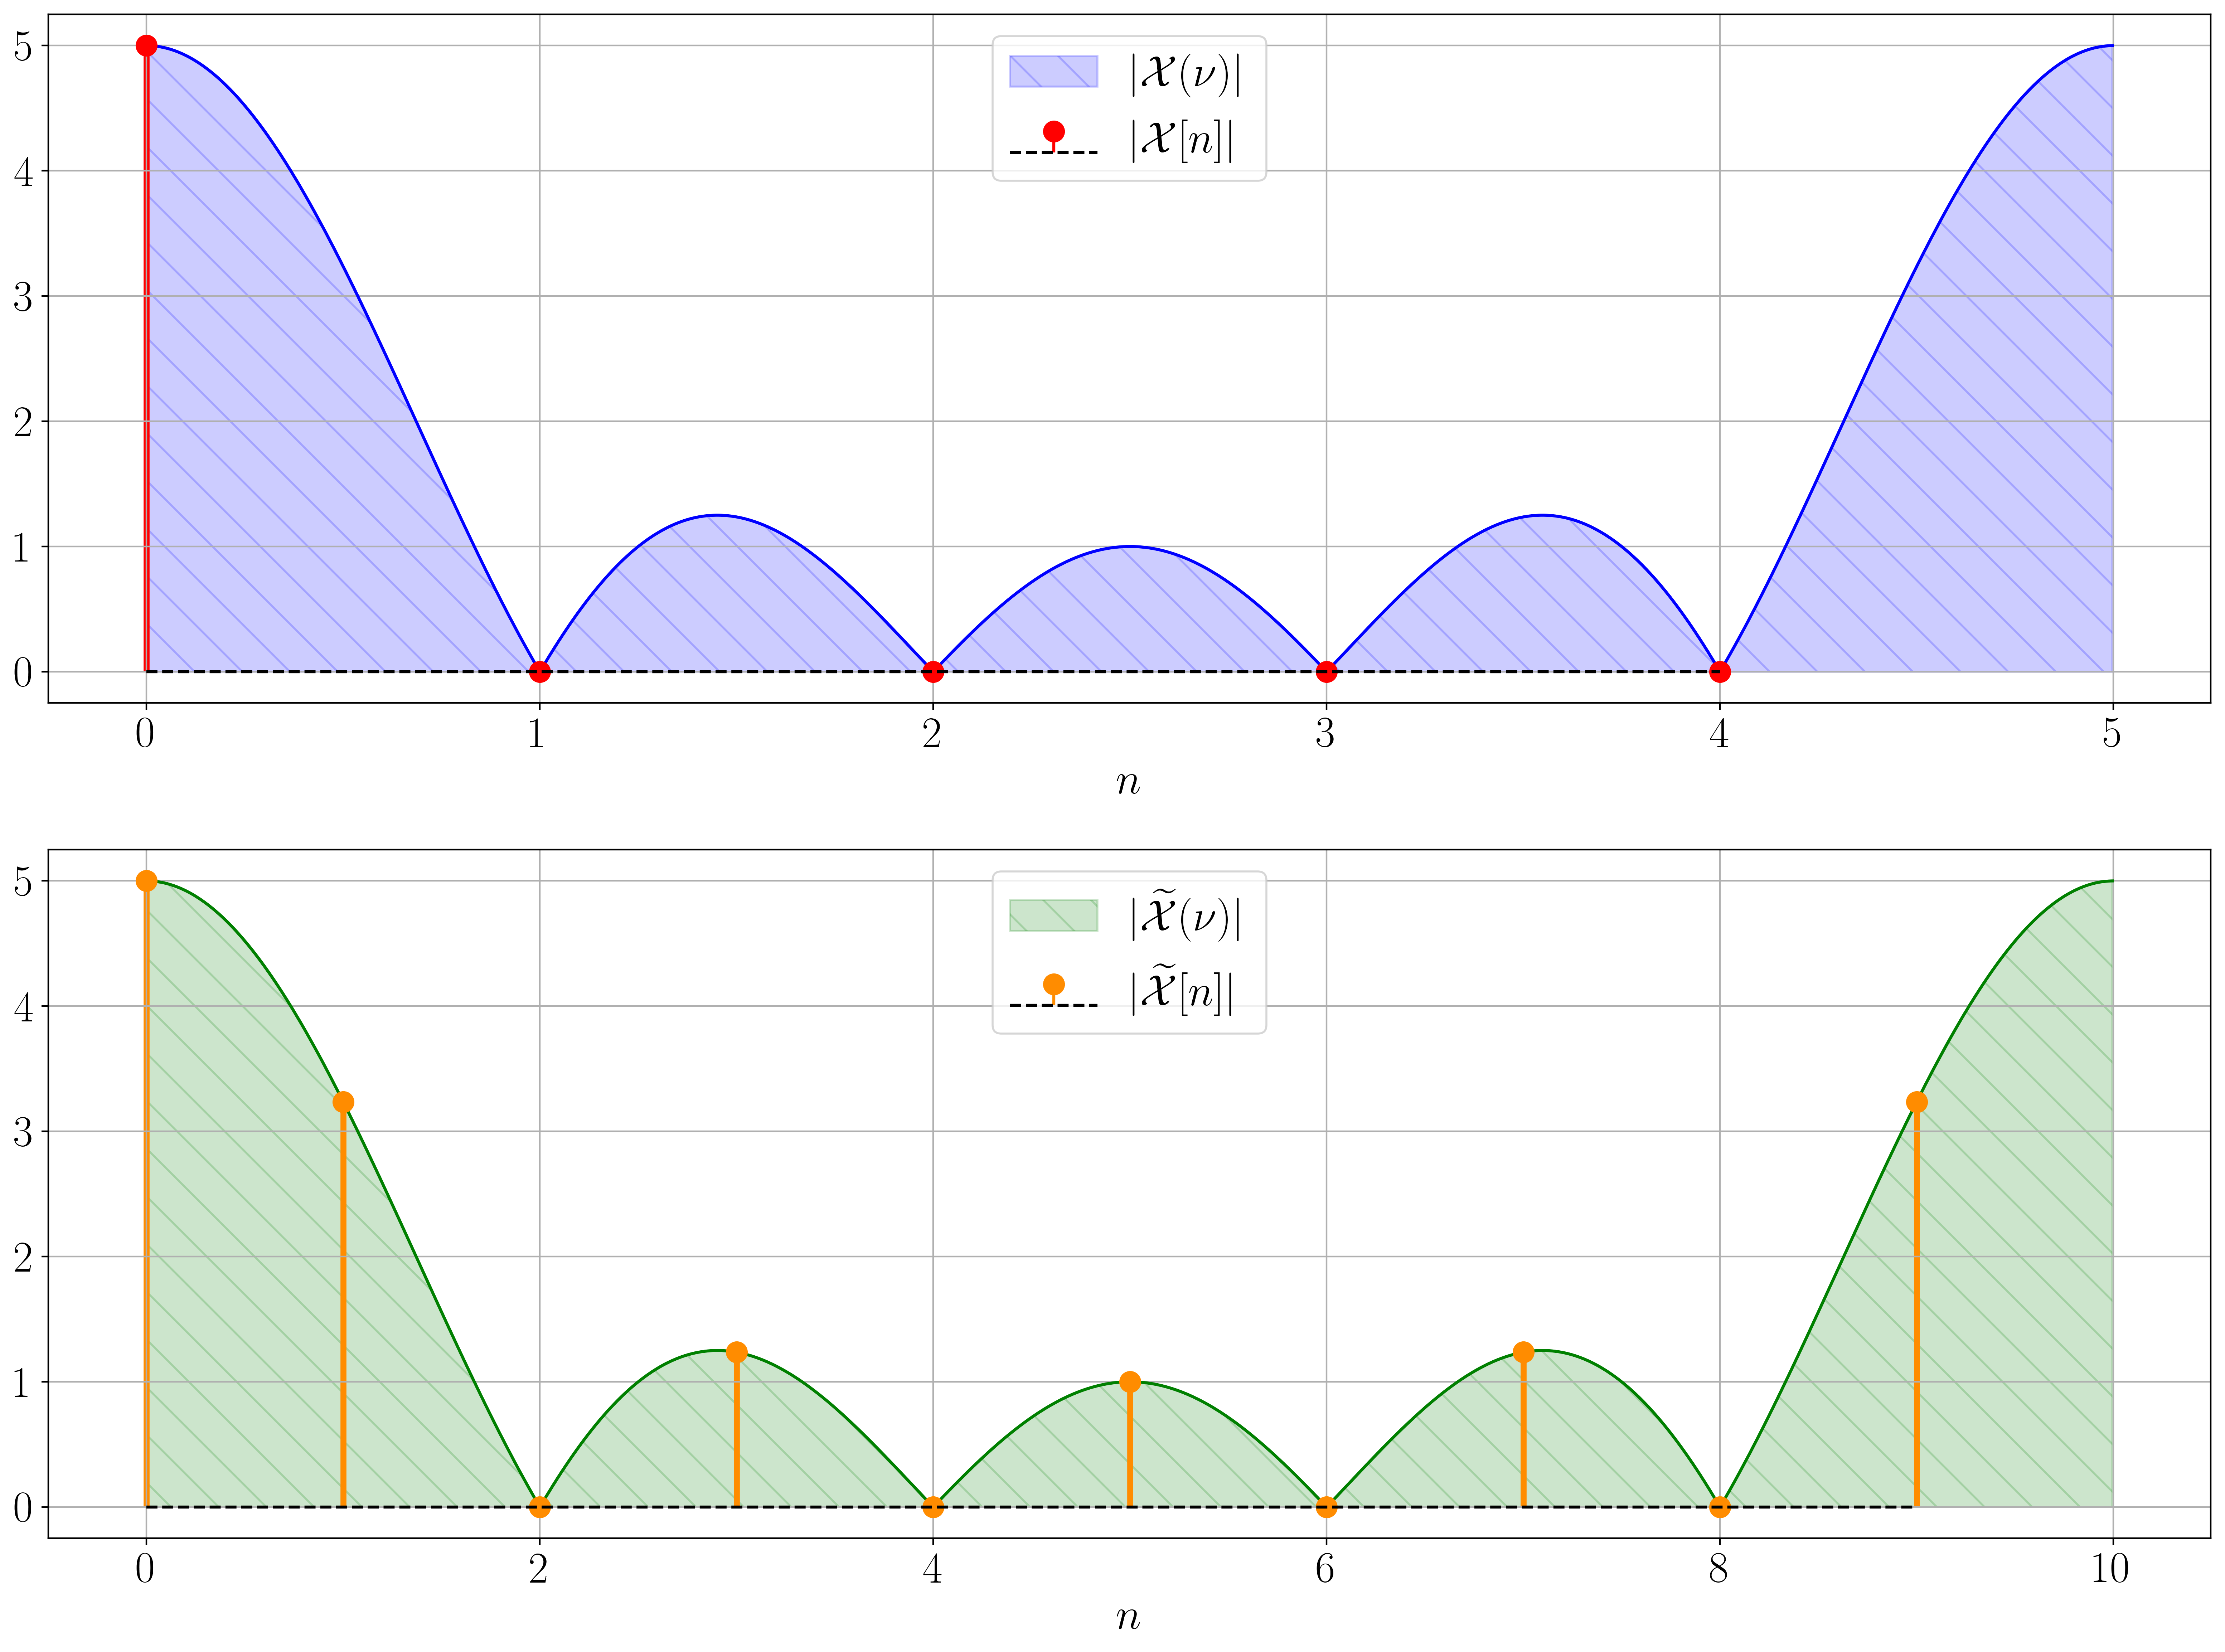
\includegraphics[width=0.9\columnwidth]{pics/fall/3/3-2.png}
	\label{fig:3-2}
\end{figure}


\section{}
Пусть $\Capit{X}[n]$ -- четырёхточечное ДПФ последовательности $x[k]$, изображённой на графике.

\begin{figure}[!h]
	\centering
	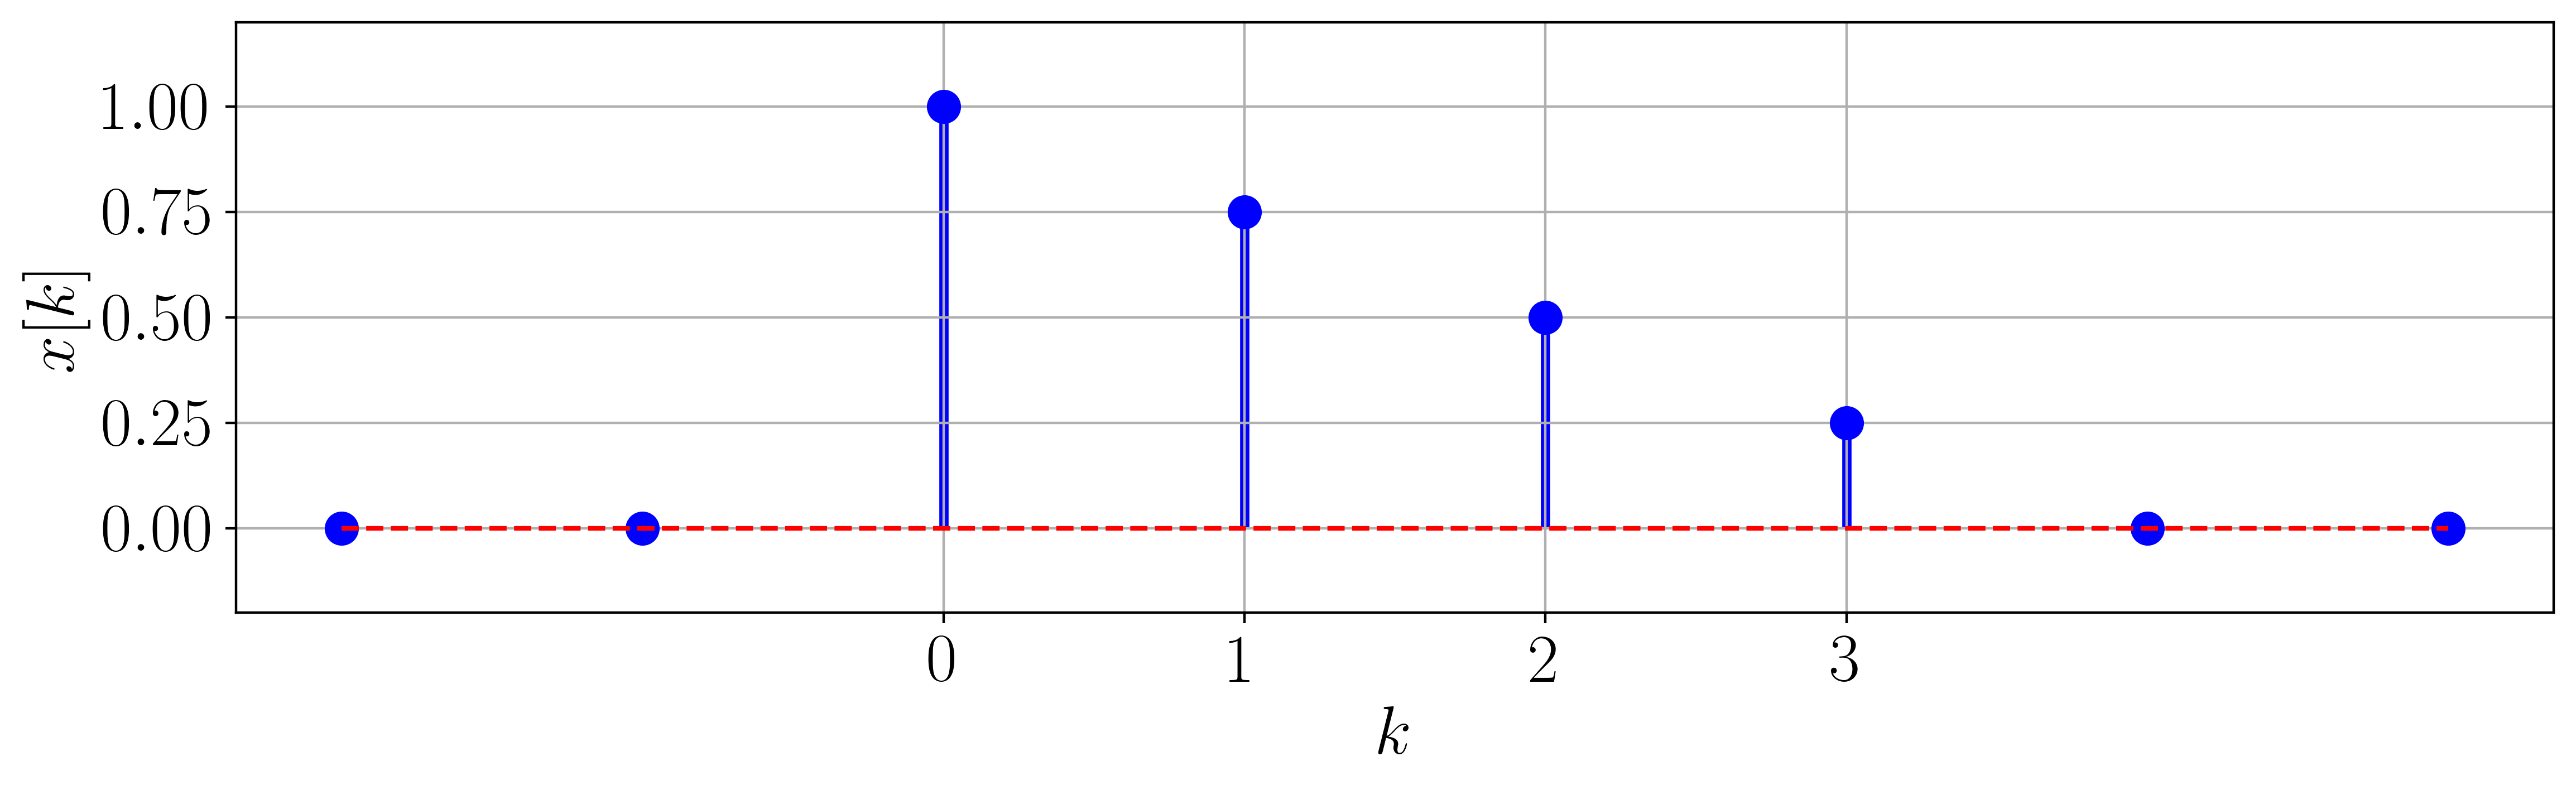
\includegraphics[width=0.8\columnwidth]{pics/fall/3/3-3-1.png}
	\label{fig:3-3-1}
\end{figure}

Изобразить последовательность $y[k]$, ДПФ которой имеет вид $\Capit{Y}[n] = \exp\Big(-j \dfrac{2\pi}{4}n\Big)\Capit{X}[n]$.

По теореме запаздывания имеем:
\begin{equation*}
	\Capit{Y}[n] = \exp\Big(-j \dfrac{2\pi}{4}n\Big)\Capit{X}[n]\ \xlongleftrightarrow{DFT}\ x[k-1]_{4} = y[k].
\end{equation*}

То есть последовательность $y[k]$ получается путём циклического сдвига $x[k]$ на $1$ отсчёт вправо.
\begin{figure}[!h]
	\centering
	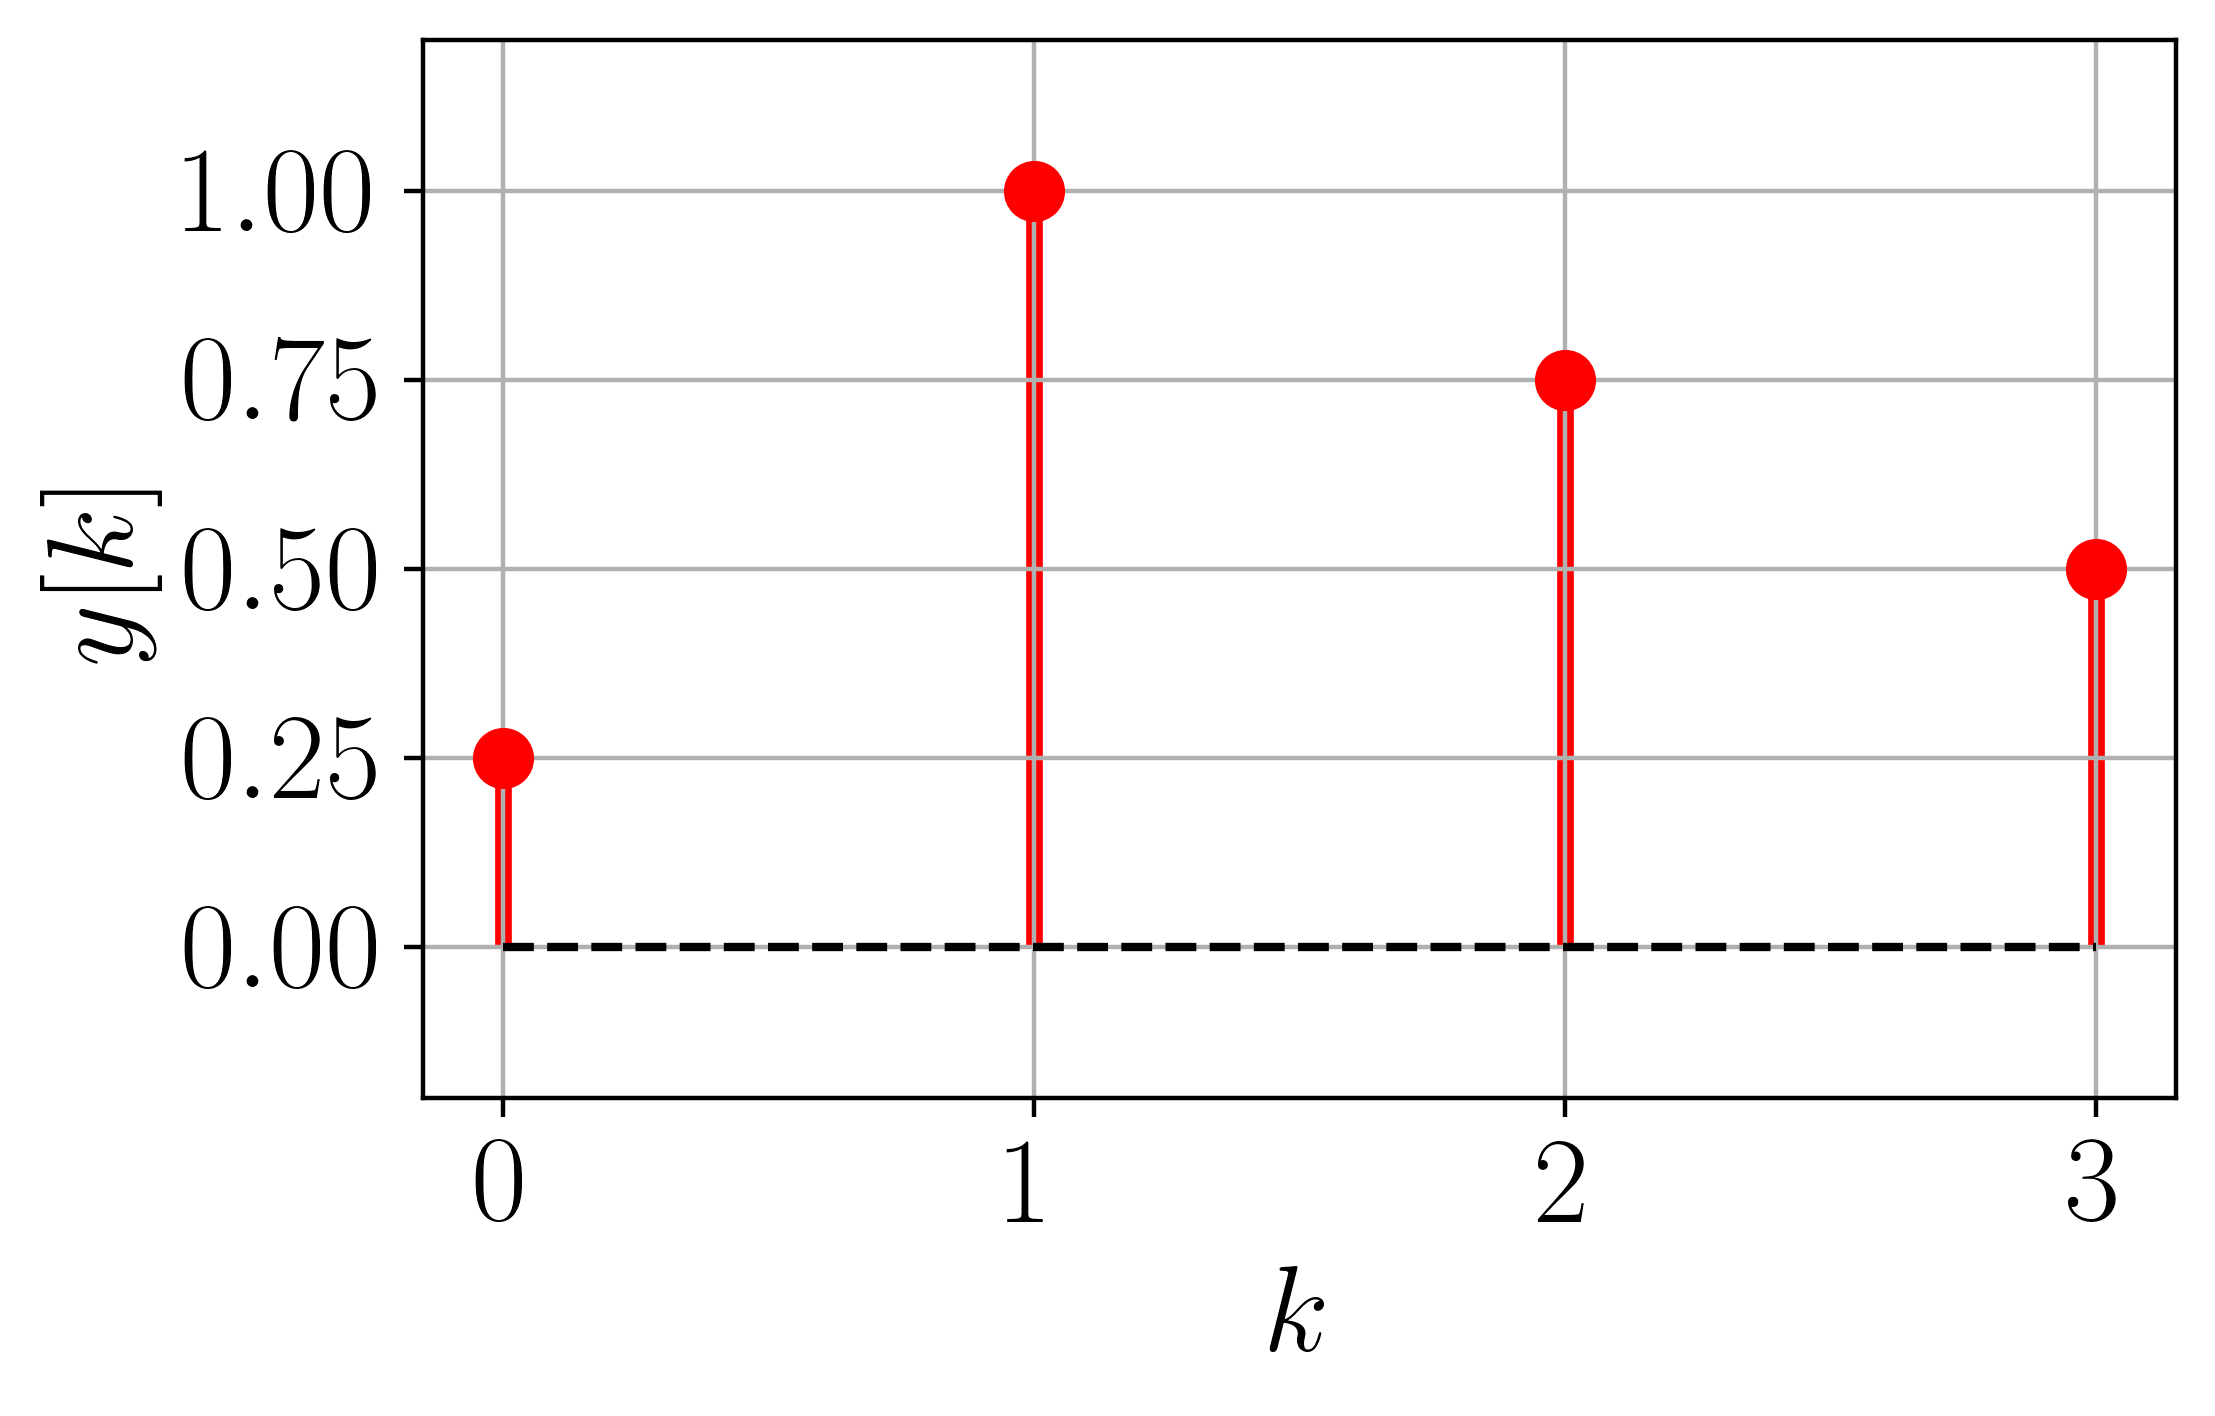
\includegraphics[width=0.4\columnwidth]{pics/fall/3/3-3-2.png}
	\label{fig:3-3-2}
\end{figure}


\setcounter{chapter}{4}
\setcounter{section}{0}
%\chapter*{Неделя 4}
\protect\thispagestyle{fancy}
\section{}
Используется $16$-разрядный биполярный АЦП и фильтр Баттерворта третьего порядка с частотой среза $f_c = 10$ КHz и амплитудно частотной характеристикой:
\[|\Capit{H}(f)| = \dfrac{1}{\sqrt{1 + (f/f_c)^6}}.\]

Предположим, что входной сигнал является широкополосным.

Оценить минимальное затухание в полосе подавления $\Capit{A}_{\min}$ для фильтра защиты от наложения.

Оценить минимальную частоту дискретизации $f_d$.

Используя формулу для относительного шума квантования, получим:
\begin{align*}
	\Capit{A}_{\min} = -\gamma_{16} = (6.02n + 1.76)\Big|_{n=16} = 98.08 \text{ dB}.
\end{align*}

\begin{equation*}
	\dfrac{1}{\Capit{A}^2_{\min}} = \dfrac{1}{1 + \left(f_{\max}/f_c\right)^6}, \quad \Rightarrow
	f_{\max} = f_c \sqrt[6]{\Capit{A}^2_{\min} - 1} \approx f_c \cdot \Capit{A}^{1/3}_{\min} = 10^{\frac{98.08}{3 \cdot 20}} \cdot f_c \approx 43.12 f_c \approx 431.2 \text{ KHz}.
\end{equation*}
\begin{equation*}
	f_d = 2f_{\max} = 862.2 \text{ KHz}.
\end{equation*}

\section{}
Аналоговый фильтр Чебышёва I рода $3$-го порядка с частотой среза $f_c = 40$ Hz имеет величину пульсаций $0.5$ dB. Определить ослабление, вносимое этим фильтром на частоте $2f_c$.

\begin{align*}
	&|\Capit{H}(\nu_c)|^2 = 10 \lg \dfrac{1}{1 + \varepsilon^2 \Capit{T}^2_3 (\nu_c)} = -0.5 \text{ dB}, \quad \Rightarrow
	\varepsilon^2 = \dfrac{10^{0.5/10} - 1}{\Capit{T}^2_3(\nu_c)} = 10^{0.05} - 1 = 0.122018.\\
	&|\Capit{H}(2\nu_c)|^2 = 10 \lg \dfrac{1}{1 + \varepsilon^2 \Capit{T}^2_3 (2\nu_c)}\footnotemark = 
	10 \lg \dfrac{1}{1 + \varepsilon^2 [4(2\nu_c)^3 - 3(2\nu_c)]^2} =
	10 \lg \dfrac{1}{1 + 0.122018 \cdot 26^2} = -19.216 \text{ dB}.
\end{align*}
\footnotetext{$\Capit{T}_3(\nu) = 2\nu \Capit{T}_2(\nu) - \Capit{T}_1 (\nu)  =  2\nu[2\nu \Capit{T}_1(\nu) - \Capit{T}_0 (\nu)] - \Capit{T}_1 (\nu) = 4\nu^3 - 3\nu$.}

\section{}
Вещественный сигнал $x(t)$ с полосой $2f_b = 10$ KHz ($f_b$ -- верхняя граничная частота) дискретизуется с минимально возможной частотой дискретизации в соответствии с теоремой отсчётов. В результате получается последовательность $x(k)$. Обозначим через $\Capit{X}[n]$ $1000$-точечное ДПФ последовательности $x(k)$.

\begin{enumerate}[label=(\alph*)]
	\item Каким частотам (в Hz) в ДВПФ последовательности $x(k)$ соответствуют частоты ДПФ с номерами $n_1 = 100$ и $n_2 = 850$?
	
	\item Каким частотам (в Hz) в спектре исходного сигнала $x(t)$ соответствуют индексы $n_1 = 100$ и $n_2 = 850$ в последовательности $\Capit{X}[n]$?
\end{enumerate}

Частота дискретизации должна быть равна $f_d = 2f_b = 10$ KHz.

\begin{enumerate}[label=(\alph*)]
	\item Для дискретизованного сигнала:
	\begin{align*}
		f_1 = \dfrac{n_1 f_d}{N} = 1\text{ KHz}, \quad f_2 = \dfrac{n_2 f_d}{N} = 8.5\text{ KHz}.
	\end{align*}
	\item Для исходного аналогового сигнала:
	\begin{align*}
		f_1 = \dfrac{n_1 f_d}{N} = 1\text{ KHz}, \quad f_2 = \dfrac{(n_2 - N)f_d}{N} = -1.5\text{ KHz}.
	\end{align*}
\end{enumerate}


\setcounter{chapter}{5}
\setcounter{section}{0}
%\chapter*{Неделя 5}
\protect\thispagestyle{fancy}
\section{}
Рассмотрим сигнал $y(t)$, полученный путём фиксации на время, равное шагу дискретизации $\Delta t$, мгновенных значений исходного сигнала $x(t)$ с помощью ЦАП.

\begin{figure}[!h]
	\centering
	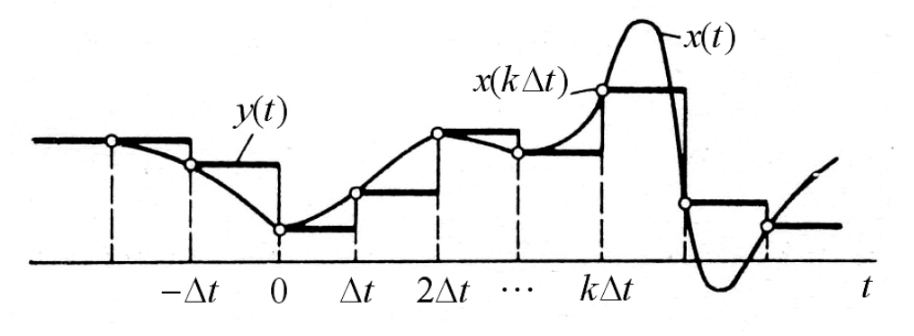
\includegraphics[width=0.5\columnwidth]{pics/fall/5/DAC.png}
	\label{fig:5-1}
\end{figure}

Пусть $x(t) = \sin(2\pi f_0 t)$, $-\infty < t < +\infty$ и шаг дискретизации $\Delta t = \frac{1}{10 f_0} = \frac{1}{f_d}$.

Определить частоты, амплитуды и фазы гармонических компонент на выходе фиксатора. Получить аналитическое выражения для выходного сигнала фиксатора как суперпозицию этих компонент.

Частотная характеристика интерполятора:
\begin{equation*}
	\Capit{H}(f) = \dfrac{\sin(\pi f \Delta t)}{\pi f} e^{-j \pi f \Delta t} = 
	\dfrac{\sin(\pi f/f_d)}{\pi f} e^{-j \pi f / f_d}.
\end{equation*}

Спектр дискретизованного сигнала на входе:
\begin{equation*}
	\Capit{X}_{d}(f) = \dfrac{1}{2j} \sum \limits_{m = -\infty}^{+\infty} 
	\big[\delta(f - f_0 + m f_d) - \delta(f + f_0 + m f_d)\big].
\end{equation*}

Спектр выходного сигнала (по теореме о свёртке):
\begin{equation*}
	\Capit{Y}(f) = \Capit{H}(f) \cdot \Capit{H}_{d}(f) = \dfrac{\sin(\pi f/f_d)}{\pi f} \dfrac{e^{-j \pi f / f_d}}{2 j} \sum \limits_{m = -\infty}^{+\infty} 
	\big[\delta(f - f_0 + m f_d) - \delta(f + f_0 + m f_d)\big].
\end{equation*}

Выходной сигнал:

\begin{align*}
	y(t)&=\int\limits_{-\infty}^{+\infty} \Delta t \dfrac{\sin (\pi f / f_{d})}{\pi f / f_{d}} \dfrac{e^{-j \pi f / f_{\mathrm{d}}}}{2 j} 
	\sum \limits_{m = -\infty}^{+\infty} 
	\big[\delta(f - f_0 + m f_d) - \delta(f + f_0 + m f_d)\big] e^{j 2 \pi f} d f=\\
	&=\sum_{m=-\infty}^{+\infty} \Delta t \left\{\dfrac{\sin \left(\pi\left(f_{0}+m f_{d}\right) / f_{d}\right)}{\pi\left(f_{0} + m f_{d}\right) / f_{d}}\right\}
	\sin \Big(2 \pi\left(f_{0}+m f_{d}\right) t -\pi\left(f_{0}+m f_{d}\right) / f_{d}\Big)=\\
	&=\sum_{m=-\infty}^{+\infty} \Delta t \left\{\dfrac{\sin \left(\pi\left(f_{0} +m f_{d}\right) / f_{d}\right)}{\pi\left(f_{d} + m f_{d}\right) / f_{d}}\right\}
	\sin \left(2 \pi \left(f_0 + m f_d\right) \left(t - \frac{1}{2} \Delta t\right)\right)=\\
	&=\sum_{m=-\infty}^{+\infty} \dfrac{1}{10 f_0} \left\{\dfrac{\sin \left(\pi\left(m + 0.1\right)\right)}{\pi\left(m + 0.1\right)}\right\}
	\sin \left(2 \pi f_0 \left(1 + 10m\right) \left(t - \frac{1}{20f_0}\right)\right).
\end{align*}

Выходной сигнал представляет собой суперпозицию гармоник:
\begin{itemize}
	\item с частотами $f_{m} = f_0 (1 + 10m)$,
	\item с амплитудами $\Capit{A}_m = \left|\dfrac{1}{10 f_0} \dfrac{\sin \left(\pi\left(m + 0.1\right)\right)}{\pi\left(m + 0.1\right)} \right|$,
	\item с фазами $\phi_m = -\pi (m + 0.1)$.
\end{itemize}



\section{}
Последовательность $x[k]$ из $1000$ элементов получена в результате дискретизации непрерывного сигнала $x(t)$ с частотой $f_d = 20480$ Hz. Обозначим через $\Capit{X}[n]$ $1024$-точечное ДПФ ($N = 1024$) последовательности $x[k]$ (дополненной нулевыми отсчётами). 
Определить расстояние (в Hz) между непрерывными частотами, которые соответствуют соседним отсчётам ДПФ.

Расстояние между соседними бинами ДПФ равно:
\begin{equation*}
	\Delta f  = \dfrac{1}{N} f_d = \dfrac{20480\text{ Hz}}{1024} = 20\text{ Hz.}
\end{equation*}

\section{}
Вещественный сигнал $x(t)$ с полосой $2f_b = 10$ KHz ($f_b$ -- верхняя граничная частота) дискретизуется с шагом $\Delta t$. В результате получается последовательность отсчётов $x[k]$. Вычисляется $N$-точечное ДПФ, где $N = 2^m$, $m \in \mathbb{N}$.

Определить минимальное значение $m$, при котором анализ возможен, а расстояние между отсчётами ДПФ по оси частот в герцах будет меньше $5$ Hz. Для этого значения $m$ определить допустимые пределы для частоты дискретизации $f_{\min} < f_d < f_{\max}$.

Чтобы разрешение по частоте оказалось меньше $\Delta f = 5$ Hz, необходимо:
\begin{align*}
	\Delta f > \dfrac{f_d}{N} = \dfrac{f_d}{2^m}\quad \Leftrightarrow \quad m > \log_2 \left( \frac{f_d}{\Delta f} \right).
\end{align*}

Чтобы анализ был возможен $f_d = f_{\min} = 2f_b = 10$ KHz, тогда $m = 11$.

Теперь для фиксированного $m$ найдём максимально возможную частоту дискретизации $f_d = f_{\max}$:
\begin{equation*}
	\Delta f > \dfrac{f_d}{N} = \dfrac{f_d}{2^m}\quad \Leftrightarrow \quad f_d < \Delta f \cdot 2^m  = 10240\text{ Hz.}
\end{equation*}

В итоге: $m = 11$, $f_{\min} = 10000$ Hz, $f_{\max} = 10240$ Hz.


\setcounter{chapter}{7}
\setcounter{section}{0}
%\chapter*{Неделя 7}
\protect\thispagestyle{fancy}
\section{}
Используя теорему о свёртке во временной области для ДВПФ, определите линейную дискретную свёртку последовательностей:

\begin{align*}
	h[k] = \dfrac{\sin(2 \pi \nu_c k)}{\pi k},\quad \nu_c = 0.2;\quad x[k] = \cos(2\pi \nu_1 k) + \cos(2 \pi \nu_2 k), \quad \nu_1 = 0.1,\; \nu_2 = 0.3.
\end{align*}

Интерпретируйте результат как прохождение сигнала $x[k]$ через фильтр с импульсной характеристикой $h[k]$. Является ли такой фильтр $h[k]$ физически реализуемым?

\begin{equation*}
	h[k] \xlongleftrightarrow{DTFT} \Capit{H}(\nu) = \Theta\left(|\nu| \leq \nu_c\right) = 
	\begin{cases}
		1,& \text{если } m-\nu_c \leq \nu \leq m+\nu_c,\; m\in\mathbb{Z},\\
		0,& \text{иначе.}
	\end{cases}
\end{equation*}

\begin{equation*}
	x[k] \xlongleftrightarrow{DTFT} \Capit{X}(\nu) = \dfrac{1}{2}\sum\limits_{m = \infty}^{+\infty}
	\left[\delta(\nu - \nu_1 + m) + \delta(\nu + \nu_1 + m) + \delta(\nu - \nu_2 + m) + \delta(\nu + \nu_2 + m)\right].
\end{equation*}

\begin{align*}
	\Capit{Y}(\nu) &= \Capit{X}(\nu) \cdot \Capit{H}(\nu) = \dfrac{1}{2}\sum\limits_{m = -\infty}^{+\infty}
	\Theta_m\left(|\nu| \leq \nu_c\right) \left[\delta(\nu - \nu_1 + m) + \delta(\nu + \nu_1 + m) + \delta(\nu - \nu_2 + m) + \delta(\nu + \nu_2 + m)\right] = \\
	&= \Big\slash \nu_1 < \nu_c,\; \nu_c < \nu_2 \Big\slash = \dfrac{1}{2}\sum\limits_{m = -\infty}^{+\infty}
	\left[\delta(\nu - \nu_1 + m) + \delta(\nu + \nu_1 + m)\right] \xlongleftrightarrow{DTFT} 
	y[k] = \cos(2 \pi \nu_1 k) = h[k] \otimes x[k].
\end{align*}

Мы имеем дело с идеальным фильтром нижних частот.
Заметим, что $h[k]$ некаузальна (не обращается тождественно в нуль при $k<0$, т.е. ее выходное воздействие зависит в том числе и от <<будущего>>). Это означает, что идеальный фильтр нижних частот физически не реализуем в системе реального времени. 


\section{}
Запишите импульсные характеристики перечисленных ниже фильтров. Являются ли такие фильтры физически реализуемыми в реальном времени?

\begin{itemize}
	\item Идеальный режекторный фильтр, частотная характеристика которого изображена на рисунке.
	\begin{figure}[!h]
		\centering
		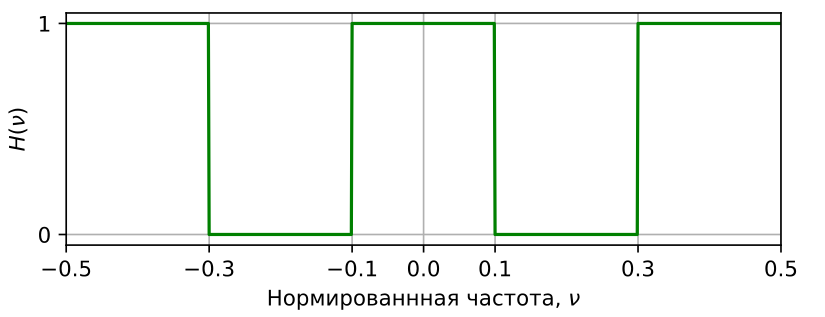
\includegraphics[width=0.6\columnwidth]{pics/fall/7/7-1.png}
		\label{fig:7-1}
		
	\end{figure}
	
\end{itemize}

Заметим, что $\Capit{H}(\nu) = 1 - \Capit{H}_{\ell}^{\nu_1}(\nu) + \Capit{H}_{\ell}^{\nu_2}(\nu)$, где $\Capit{H}_{\ell}^{\nu_c}(\nu)$ -- частотная характеристика идеального фильтра нижних частот с частотой среза $\nu_c$, $\nu_1 = 0.3$ и $\nu_2 = 0.1$. 
В силу линейности ДВПФ справедливо, что $h[k] = \mathbf{1}[k] - h_{\ell}^{\nu_1}[k] + h_{\ell}^{\nu_2}[k]$, где $h_{\ell}^{\nu_c}[k]$ -- импульсная характеристика идеального фильтра нижних частот с частотой среза $\nu_c$. В итоге получим:


\begin{equation*}
	h[k] = \mathbf{1}[k] - h_{\ell}^{\nu_1}[k] + h_{\ell}^{\nu_2}[k] =
	\mathbf{1}[k] - \dfrac{\sin(2 \pi \nu_1 k)}{\pi k} + \dfrac{\sin(2 \pi \nu_2 k)}{\pi k} = 
	\mathbf{1}[k] - \dfrac{2\sin\left(\pi(\nu_1 - \nu_2)k\right)\cos\left(\pi(\nu_1 + \nu_2)k\right)}{\pi k}.
\end{equation*}

$h[k]$ не обращается тождественно в нуль при $k<0$, т.е. не является каузальной. Это означает, что данный фильтр физически не реализуем в системе реального времени. 

\begin{itemize}
	
	\item Идеальный фильтр с нулевой фазовой задержкой, частотная характеристика которого изображена на рисунке.
	\begin{figure}[!h]
		\centering
		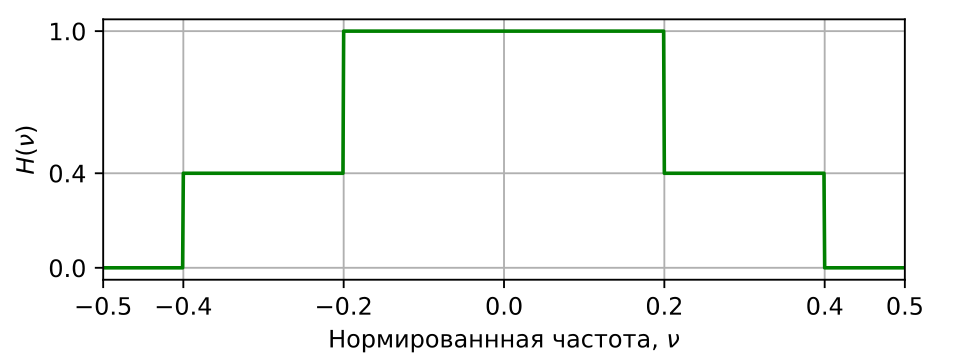
\includegraphics[width=0.6\columnwidth]{pics/fall/7/7-2.png}
		\label{fig:7-2}
	\end{figure}
\end{itemize}

Заметим, что $\Capit{H}(\nu) = 0.4\cdot \Capit{H}_{\ell}^{\nu_1}(\nu) + 0.6 \cdot \Capit{H}_{\ell}^{\nu_2}(\nu)$, где $\nu_1 = 0.4$ и $\nu_2 = 0.2$. 
В силу линейности ДВПФ справедливо, что $h[k] = 0.4 \cdot h_{\ell}^{\nu_1}[k] + 0.6\cdot h_{\ell}^{\nu_2}[k]$. В итоге получим:

\begin{equation*}
	h[k] = 0.4 \cdot h_{\ell}^{\nu_1}[k] + 0.6\cdot h_{\ell}^{\nu_2}[k] = \dfrac{4\sin(2 \pi \nu_1 k) + 6\sin(2 \pi \nu_2 k)}{10\pi k}.
\end{equation*}

$h[k]$ не обращается тождественно в нуль при $k<0$, т.е. не является каузальной. Это означает, что данный фильтр физически не реализуем в системе реального времени. 


\section{}
Определить реакцию на входное воздействие $x[k] = \cos(2\pi \nu_1 k) + \cos(2 \pi \nu_2 k)$, $\nu_1 = 0.1$, $\nu_2 = 0.3$ системы с нулевой фазовой задержкой и амплитудно-частотной характеристикой, изображённой на рисунке (частотная характеристика принимает неотрицательные значения).
\begin{figure}[!h]
	\centering
	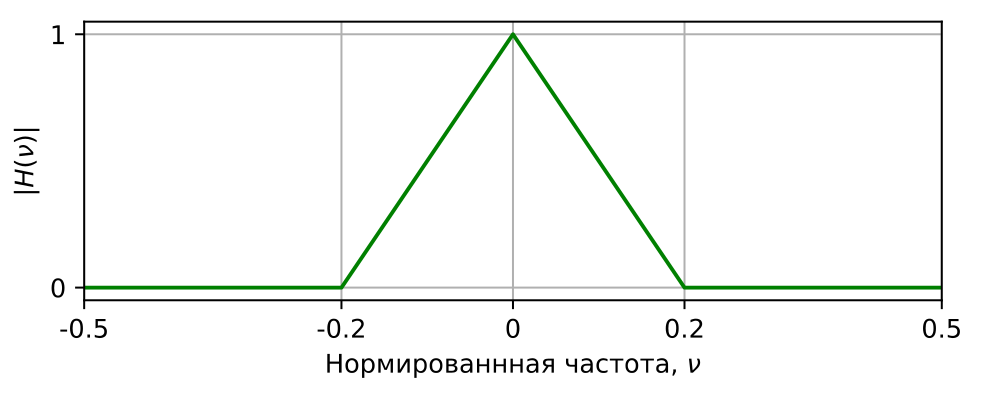
\includegraphics[width=0.6\columnwidth]{pics/fall/7/7-3.png}
	\label{fig:7-3}
\end{figure}

\begin{equation*}
	x[k] \xlongleftrightarrow{DTFT} \Capit{X}(\nu) = \dfrac{1}{2}\sum\limits_{m = \infty}^{+\infty}
	\left[\delta(\nu - \nu_1 + m) + \delta(\nu + \nu_1 + m) + \delta(\nu - \nu_2 + m) + \delta(\nu + \nu_2 + m)\right].
\end{equation*}

\begin{align*}
	\Capit{Y}(\nu) &= \Capit{X}(\nu) \cdot \Capit{H}(\nu) = \dfrac{1}{2}\sum\limits_{m = -\infty}^{+\infty}
	\Capit{X}(\nu) \left[\delta(\nu - \nu_1 + m) + \delta(\nu + \nu_1 + m) + \delta(\nu - \nu_2 + m) + \delta(\nu + \nu_2 + m)\right] = \\
	&= \Big\slash \Capit{X}(\nu_1) = \frac{1}{2},\; \Capit{X}(\nu_2) = 0 \Big\slash = \dfrac{1}{4}\sum\limits_{m = -\infty}^{+\infty}
	\left[\delta(\nu - \nu_1 + m) + \delta(\nu + \nu_1 + m)\right] \xlongleftrightarrow{DTFT} 
	y[k] = \dfrac{1}{2}\cos(2 \pi \nu_1 k).
\end{align*}


\setcounter{chapter}{8}
\setcounter{section}{0}
%\chapter*{Неделя 7}
\protect\thispagestyle{fancy}
\section{}
Используя теорему о свёртке во временной области для ДВПФ, определите линейную дискретную свёртку последовательностей:

\begin{align*}
	h[k] = \dfrac{\sin(2 \pi \nu_c k)}{\pi k},\quad \nu_c = 0.2;\quad x[k] = \cos(2\pi \nu_1 k) + \cos(2 \pi \nu_2 k), \quad \nu_1 = 0.1,\; \nu_2 = 0.3.
\end{align*}

Интерпретируйте результат как прохождение сигнала $x[k]$ через фильтр с импульсной характеристикой $h[k]$. Является ли такой фильтр $h[k]$ физически реализуемым?

\begin{equation*}
	h[k] \xlongleftrightarrow{DTFT} \Capit{H}(\nu) = \Theta\left(|\nu| \leq \nu_c\right) = 
	\begin{cases}
		1,& \text{если } m-\nu_c \leq \nu \leq m+\nu_c,\; m\in\mathbb{Z},\\
		0,& \text{иначе.}
	\end{cases}
\end{equation*}

\begin{equation*}
	x[k] \xlongleftrightarrow{DTFT} \Capit{X}(\nu) = \dfrac{1}{2}\sum\limits_{m = \infty}^{+\infty}
	\left[\delta(\nu - \nu_1 + m) + \delta(\nu + \nu_1 + m) + \delta(\nu - \nu_2 + m) + \delta(\nu + \nu_2 + m)\right].
\end{equation*}

\begin{align*}
	\Capit{Y}(\nu) &= \Capit{X}(\nu) \cdot \Capit{H}(\nu) = \dfrac{1}{2}\sum\limits_{m = -\infty}^{+\infty}
	\Theta_m\left(|\nu| \leq \nu_c\right) \left[\delta(\nu - \nu_1 + m) + \delta(\nu + \nu_1 + m) + \delta(\nu - \nu_2 + m) + \delta(\nu + \nu_2 + m)\right] = \\
	&= \Big\slash \nu_1 < \nu_c,\; \nu_c < \nu_2 \Big\slash = \dfrac{1}{2}\sum\limits_{m = -\infty}^{+\infty}
	\left[\delta(\nu - \nu_1 + m) + \delta(\nu + \nu_1 + m)\right] \xlongleftrightarrow{DTFT} 
	y[k] = \cos(2 \pi \nu_1 k) = h[k] \otimes x[k].
\end{align*}

Мы имеем дело с идеальным фильтром нижних частот.
Заметим, что $h[k]$ некаузальна (не обращается тождественно в нуль при $k<0$, т.е. ее выходное воздействие зависит в том числе и от <<будущего>>). Это означает, что идеальный фильтр нижних частот физически не реализуем в системе реального времени. 


\section{}
Запишите импульсные характеристики перечисленных ниже фильтров. Являются ли такие фильтры физически реализуемыми в реальном времени?

\begin{itemize}
	\item Идеальный режекторный фильтр, частотная характеристика которого изображена на рисунке.
	\begin{figure}[!h]
		\centering
		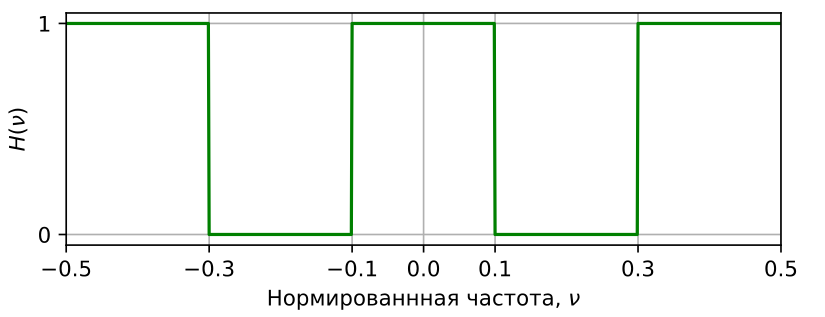
\includegraphics[width=0.6\columnwidth]{pics/fall/7/7-1.png}
		\label{fig:7-1}
		
	\end{figure}
	
\end{itemize}

Заметим, что $\Capit{H}(\nu) = 1 - \Capit{H}_{\ell}^{\nu_1}(\nu) + \Capit{H}_{\ell}^{\nu_2}(\nu)$, где $\Capit{H}_{\ell}^{\nu_c}(\nu)$ -- частотная характеристика идеального фильтра нижних частот с частотой среза $\nu_c$, $\nu_1 = 0.3$ и $\nu_2 = 0.1$. 
В силу линейности ДВПФ справедливо, что $h[k] = \mathbf{1}[k] - h_{\ell}^{\nu_1}[k] + h_{\ell}^{\nu_2}[k]$, где $h_{\ell}^{\nu_c}[k]$ -- импульсная характеристика идеального фильтра нижних частот с частотой среза $\nu_c$. В итоге получим:


\begin{equation*}
	h[k] = \mathbf{1}[k] - h_{\ell}^{\nu_1}[k] + h_{\ell}^{\nu_2}[k] =
	\mathbf{1}[k] - \dfrac{\sin(2 \pi \nu_1 k)}{\pi k} + \dfrac{\sin(2 \pi \nu_2 k)}{\pi k} = 
	\mathbf{1}[k] - \dfrac{2\sin\left(\pi(\nu_1 - \nu_2)k\right)\cos\left(\pi(\nu_1 + \nu_2)k\right)}{\pi k}.
\end{equation*}

$h[k]$ не обращается тождественно в нуль при $k<0$, т.е. не является каузальной. Это означает, что данный фильтр физически не реализуем в системе реального времени. 

\begin{itemize}
	
	\item Идеальный фильтр с нулевой фазовой задержкой, частотная характеристика которого изображена на рисунке.
	\begin{figure}[!h]
		\centering
		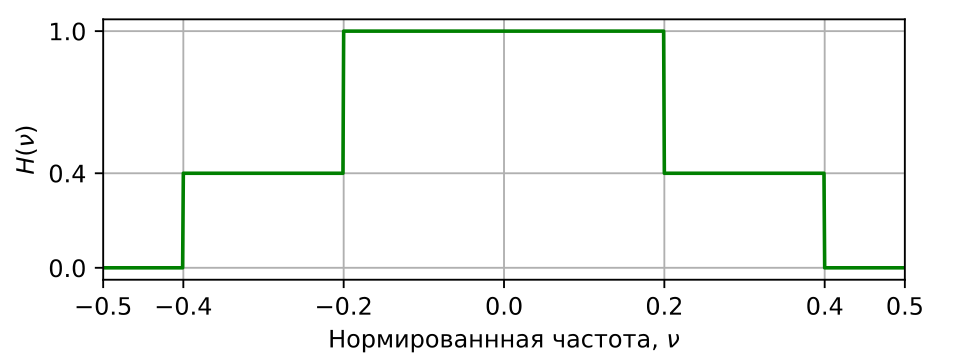
\includegraphics[width=0.6\columnwidth]{pics/fall/7/7-2.png}
		\label{fig:7-2}
	\end{figure}
\end{itemize}

Заметим, что $\Capit{H}(\nu) = 0.4\cdot \Capit{H}_{\ell}^{\nu_1}(\nu) + 0.6 \cdot \Capit{H}_{\ell}^{\nu_2}(\nu)$, где $\nu_1 = 0.4$ и $\nu_2 = 0.2$. 
В силу линейности ДВПФ справедливо, что $h[k] = 0.4 \cdot h_{\ell}^{\nu_1}[k] + 0.6\cdot h_{\ell}^{\nu_2}[k]$. В итоге получим:

\begin{equation*}
	h[k] = 0.4 \cdot h_{\ell}^{\nu_1}[k] + 0.6\cdot h_{\ell}^{\nu_2}[k] = \dfrac{4\sin(2 \pi \nu_1 k) + 6\sin(2 \pi \nu_2 k)}{10\pi k}.
\end{equation*}

$h[k]$ не обращается тождественно в нуль при $k<0$, т.е. не является каузальной. Это означает, что данный фильтр физически не реализуем в системе реального времени. 


\section{}
Определить реакцию на входное воздействие $x[k] = \cos(2\pi \nu_1 k) + \cos(2 \pi \nu_2 k)$, $\nu_1 = 0.1$, $\nu_2 = 0.3$ системы с нулевой фазовой задержкой и амплитудно-частотной характеристикой, изображённой на рисунке (частотная характеристика принимает неотрицательные значения).
\begin{figure}[!h]
	\centering
	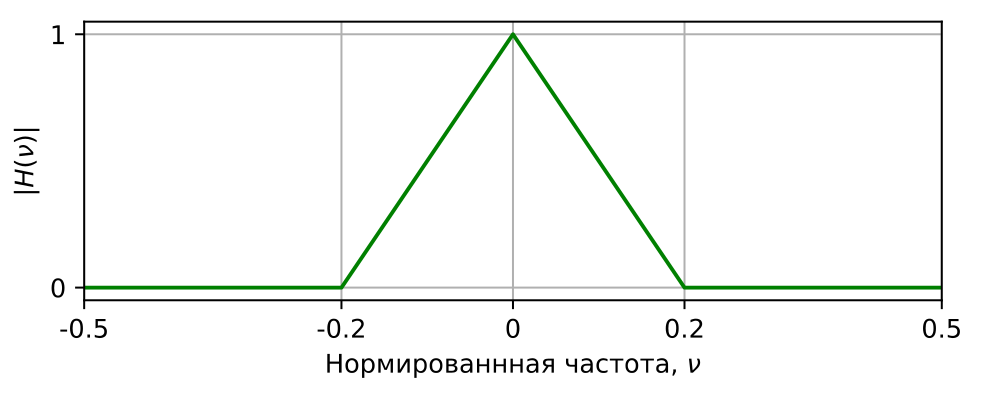
\includegraphics[width=0.6\columnwidth]{pics/fall/7/7-3.png}
	\label{fig:7-3}
\end{figure}

\begin{equation*}
	x[k] \xlongleftrightarrow{DTFT} \Capit{X}(\nu) = \dfrac{1}{2}\sum\limits_{m = \infty}^{+\infty}
	\left[\delta(\nu - \nu_1 + m) + \delta(\nu + \nu_1 + m) + \delta(\nu - \nu_2 + m) + \delta(\nu + \nu_2 + m)\right].
\end{equation*}

\begin{align*}
	\Capit{Y}(\nu) &= \Capit{X}(\nu) \cdot \Capit{H}(\nu) = \dfrac{1}{2}\sum\limits_{m = -\infty}^{+\infty}
	\Capit{X}(\nu) \left[\delta(\nu - \nu_1 + m) + \delta(\nu + \nu_1 + m) + \delta(\nu - \nu_2 + m) + \delta(\nu + \nu_2 + m)\right] = \\
	&= \Big\slash \Capit{X}(\nu_1) = \frac{1}{2},\; \Capit{X}(\nu_2) = 0 \Big\slash = \dfrac{1}{4}\sum\limits_{m = -\infty}^{+\infty}
	\left[\delta(\nu - \nu_1 + m) + \delta(\nu + \nu_1 + m)\right] \xlongleftrightarrow{DTFT} 
	y[k] = \dfrac{1}{2}\cos(2 \pi \nu_1 k).
\end{align*}


\setcounter{chapter}{9}
\setcounter{section}{0}
%\chapter*{Неделя 9}
\protect\thispagestyle{fancy}
\section{}
Пусть $\Capit{Z}$-преобразование (двухстороннее) дискретного сигнала $x[k]$ имеет вид $\Capit{X}(z) = (z^2 + 2z + 1)/z$.

Найти ненулевые отсчётные значения этого сигнала. Определить, является ли такой сигнал казуальным. 

\begin{align*}
	&\Capit{X}(z) = (z^2 + 2z + 1)/z = z + 2 + z^{-1} = x[-1]z + x[0] + x[1]z^{-1} =  \sum \limits_{-\infty}^{+\infty} x[k]z^{-k},\\
	&x[1] = x[-1] = 1,\quad x[0] = 2.
\end{align*}

При этом $x[-1] = 1 \neq 0$, то есть сигнал не является каузальным.


\section{}
Найти импульсную характеристику $h[k]$ фильтра с передаточной функцией

\begin{equation*}
	\Capit{H}(z) = \dfrac{1 - z^{-1}}{1 + 0.5z^{-1}}
\end{equation*}

\begin{enumerate}
	\item вычислением обратного $\Capit{Z}$-преобразования;
	\item реакцией на единичный импульс $\mathbf{1}[k]$ при начальном условии $y[-1]=0$.
\end{enumerate}

Сравнить результаты. Исследовать фильтр на устойчивость.

Методом геометрических построений определить значения АЧХ и ФЧХ фильтра в точке $\nu_0 = \frac{1}{4}$.

\begin{align*}
	\Capit{H}(z) = \dfrac{1 - z^{-1}}{1 + 0.5z^{-1}} = \dfrac{1}{1 + 0.5z^{-1}} - \dfrac{z^{-1}}{1 + 0.5z^{-1}} \xlongleftrightarrow{\Capit{Z}} h[k] =&\left(-\dfrac{1}{2}\right)^k \s{u}[k] -  \left(-\dfrac{1}{2}\right)^{k-1} \s{u}[k-1] = \\
	=&\left(-\dfrac{1}{2}\right)^k \left(\s{u}[k] + 2 \s{u}[k-1] \right),\quad\text{ROC} = \{z: |z| > 0.5\}.
\end{align*}

\begin{align*}
	x[k] = \mathbf{1}[k] \xlongleftrightarrow{\Capit{Z}} \Capit{X}(z) = 1,
	\quad \Capit{Y}(z) = \Capit{X}(z)\cdot \Capit{H}(z) = \Capit{H}(z) \xlongleftrightarrow{\Capit{Z}} y[k] = h[k] = \left(-\dfrac{1}{2}\right)^k \left(\s{u}[k] + 2 \s{u}[k-1] \right),\\
	\quad\text{ROC} = \{z: |z| > 0.5\}.
\end{align*}

\begin{align*}
	\Capit{H}(z) = \dfrac{1 - z^{-1}}{1 + 0.5z^{-1}} = \dfrac{z - 1}{z + 0.5},\quad
	\Rightarrow z_{\times} = -0.5, z_{o} = 1. 
\end{align*}

\begin{minipage}{0.4\textwidth}
	%\begin{figure}[!h]
	\centering
	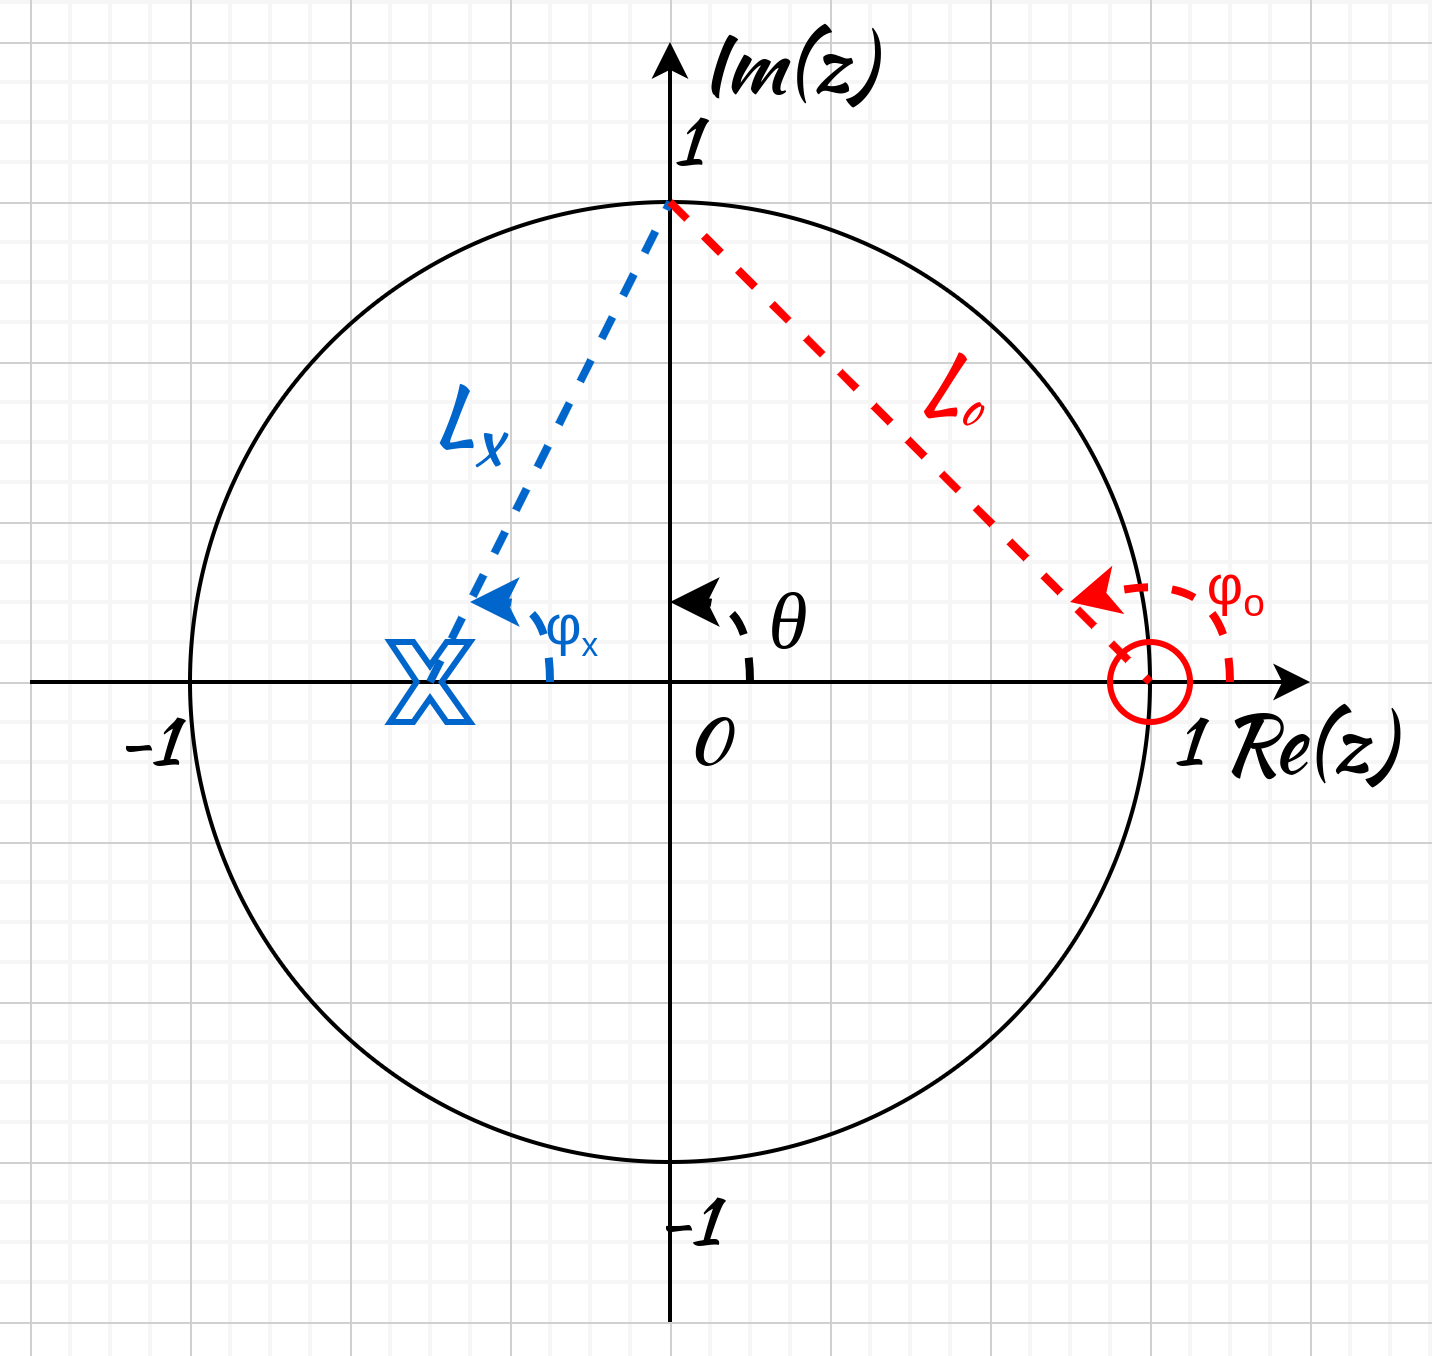
\includegraphics[width=1.\columnwidth]{pics/fall/9/complexplane.png}
	\label{fig:9-2}
	%\end{figure}
\end{minipage}
\hfill
\begin{minipage}{0.4\textwidth}
	\begin{align*}
		&\theta = 2\pi \nu_0 = 2\pi \dfrac{1}{4} = \dfrac{\pi}{2}.\\
		&\varphi(\nu_0) = \varphi(\theta) = \varphi_{o} - \varphi_{\times} = \dfrac{3\pi}{4} - \arctg(2) = 1.249 = 0.397\pi.\\
		&|\Capit{H}(\nu_0)| = |\Capit{H}(\theta)| = \dfrac{L_{o}}{L_{\times}} = \dfrac{\sqrt2}{\sqrt{1 + (0.5)^2}} = \sqrt{\dfrac{8}{5}} = 1.265.
	\end{align*}
\end{minipage}


Единственный полюс $z_{\times} = -0.5$ лежит внутри единичного круга на комплексной плоскости, то есть система является устойчивой по входу.



\section{}
Рассмотрите рекурсивный фильтр, заданный разностным уравнением

\begin{equation*}
	y[k] = (1 - \lambda)x[k] + \lambda y[k-1],\quad y[-1] = 0.
\end{equation*}

При $\lambda \approx 1$, $\lambda < 1$ эта система является квазиинтегратором (leaky integrator).
Определите импульсную характеристику этой системы и исследуйте систему на устойчивость для случаев $\lambda_1 = 1$ и $\lambda_2=0.9$.
Постройте блок-схему для реализации данной системы.

\begin{align*}
	&(1 - \lambda) x[k] = y[k] - \lambda y[k-1],\quad y[-1] = 0.\\
	&\Capit{H}(z) = \dfrac{\Capit{Y}(z)}{\Capit{X}(z)} = \dfrac{1 - \lambda}{1 - \lambda z^{-1}} =
	\dfrac{(1 - \lambda)z}{z - \lambda}  
	\xlongleftrightarrow{\Capit{Z}} h[k] = (1-\lambda)\lambda^k \s{u}[k],\quad\text{ROC} = \{z: |z| > \lambda\}.
\end{align*}

При $\lambda_1=1$ единственный полюс $z_{\times} = \lambda_1 = 1$ находится на границе единичного круга комплексной плоскости, а не внутри него. Значит, система не является устойчивой по входу.


В случае $\lambda_1=0.9$ полюс $z_{\times} = \lambda_1 = 0.9$ находится внутри единичного круга, то есть система будет устойчивой по входу.

\begin{figure}[!h]
	\centering
	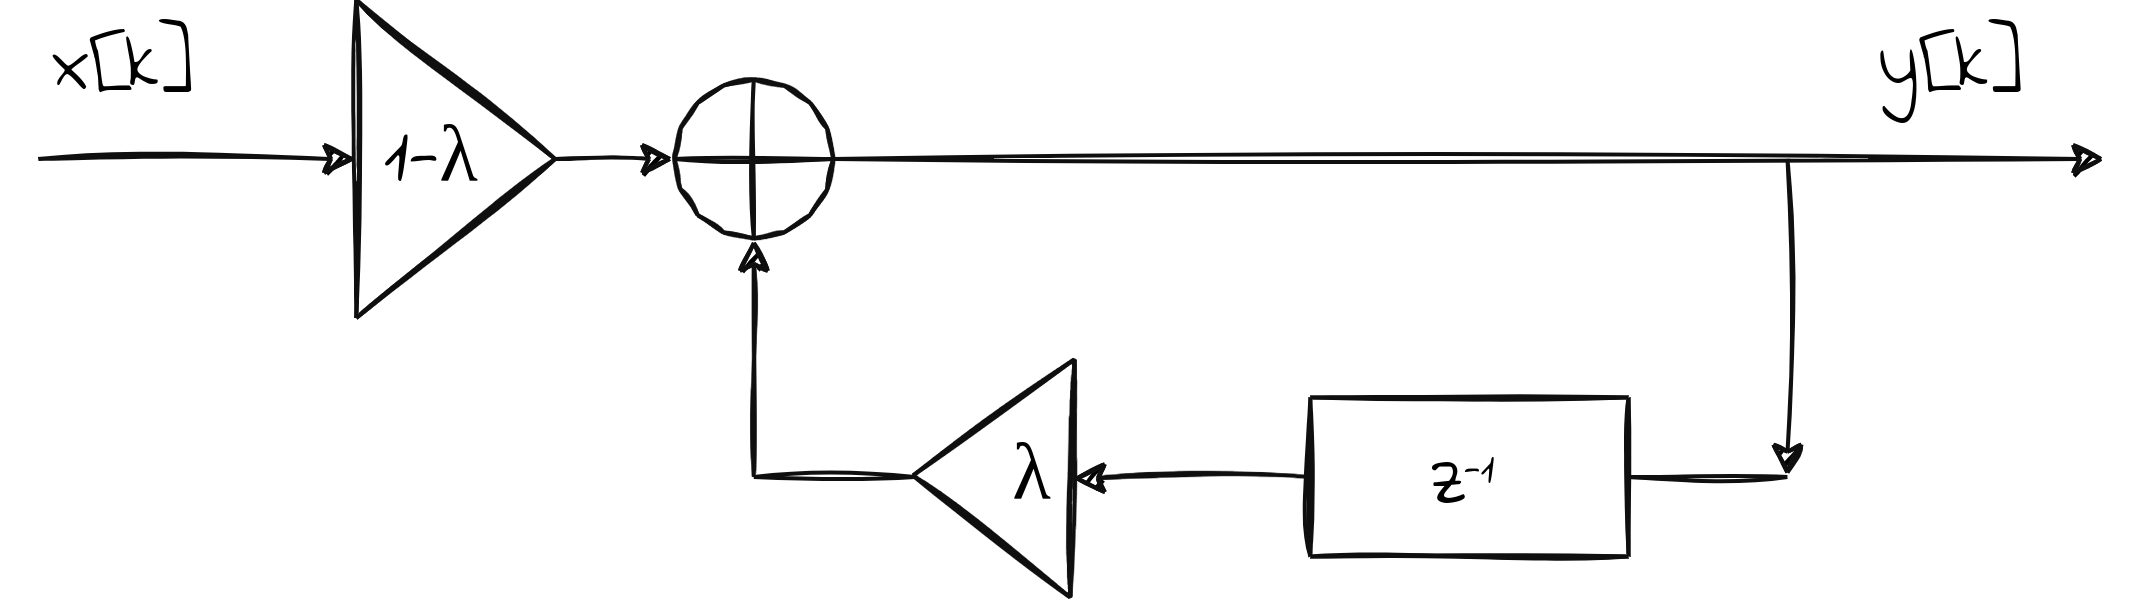
\includegraphics[width=0.8\columnwidth]{pics/fall/9/integrator.png}
	\label{fig:9-3}
\end{figure}



\setcounter{chapter}{10}
\setcounter{section}{0}
%\chapter*{Неделя 10}
\protect\thispagestyle{fancy}
\section{}
Передаточная функция цифрового фильтра имеет вид

\begin{equation*}
	\Capit{H}(z) = \dfrac{1 - 2z^{-1} + z^{-2}}{1 - \frac{1}{2}z^{-1} - \frac{1}{2}z^{-2}}.
\end{equation*}

Изобразить блок-схемы цифрового фильтра в прямой и канонической формах и записать соответствующие разностные уравнения (алгоритмы цифровой фильтрации).

\begin{align*}
	&\Capit{H}(z)\footnotemark = \dfrac{1 - 2z^{-1} + z^{-2}}{1 - \frac{1}{2}z^{-1} - \frac{1}{2}z^{-2}} = \dfrac{\Capit{Y}(z)}{\Capit{X}(z)}.\\
	\Capit{Y}(z)\Big(1 - \frac{1}{2}z^{-1} - \frac{1}{2}z^{-2}\Big) =
	\Capit{X}(z)\Big(1 &- 2z^{-1} + z^{-2}\Big) \xlongleftrightarrow{\Capit{Z}} 
	y[k] - \dfrac{1}{2}y[k-1] - \dfrac{1}{2}y[k-2] = x[k] - 2x[k-1] + x[k-2].\\
	y[k] = x[k]& - 2x[k-1] + x[k-2] + \dfrac{1}{2}y[k-1] + \dfrac{1}{2}y[k-2].
\end{align*}

\begin{figure}[!h]
	\centering
	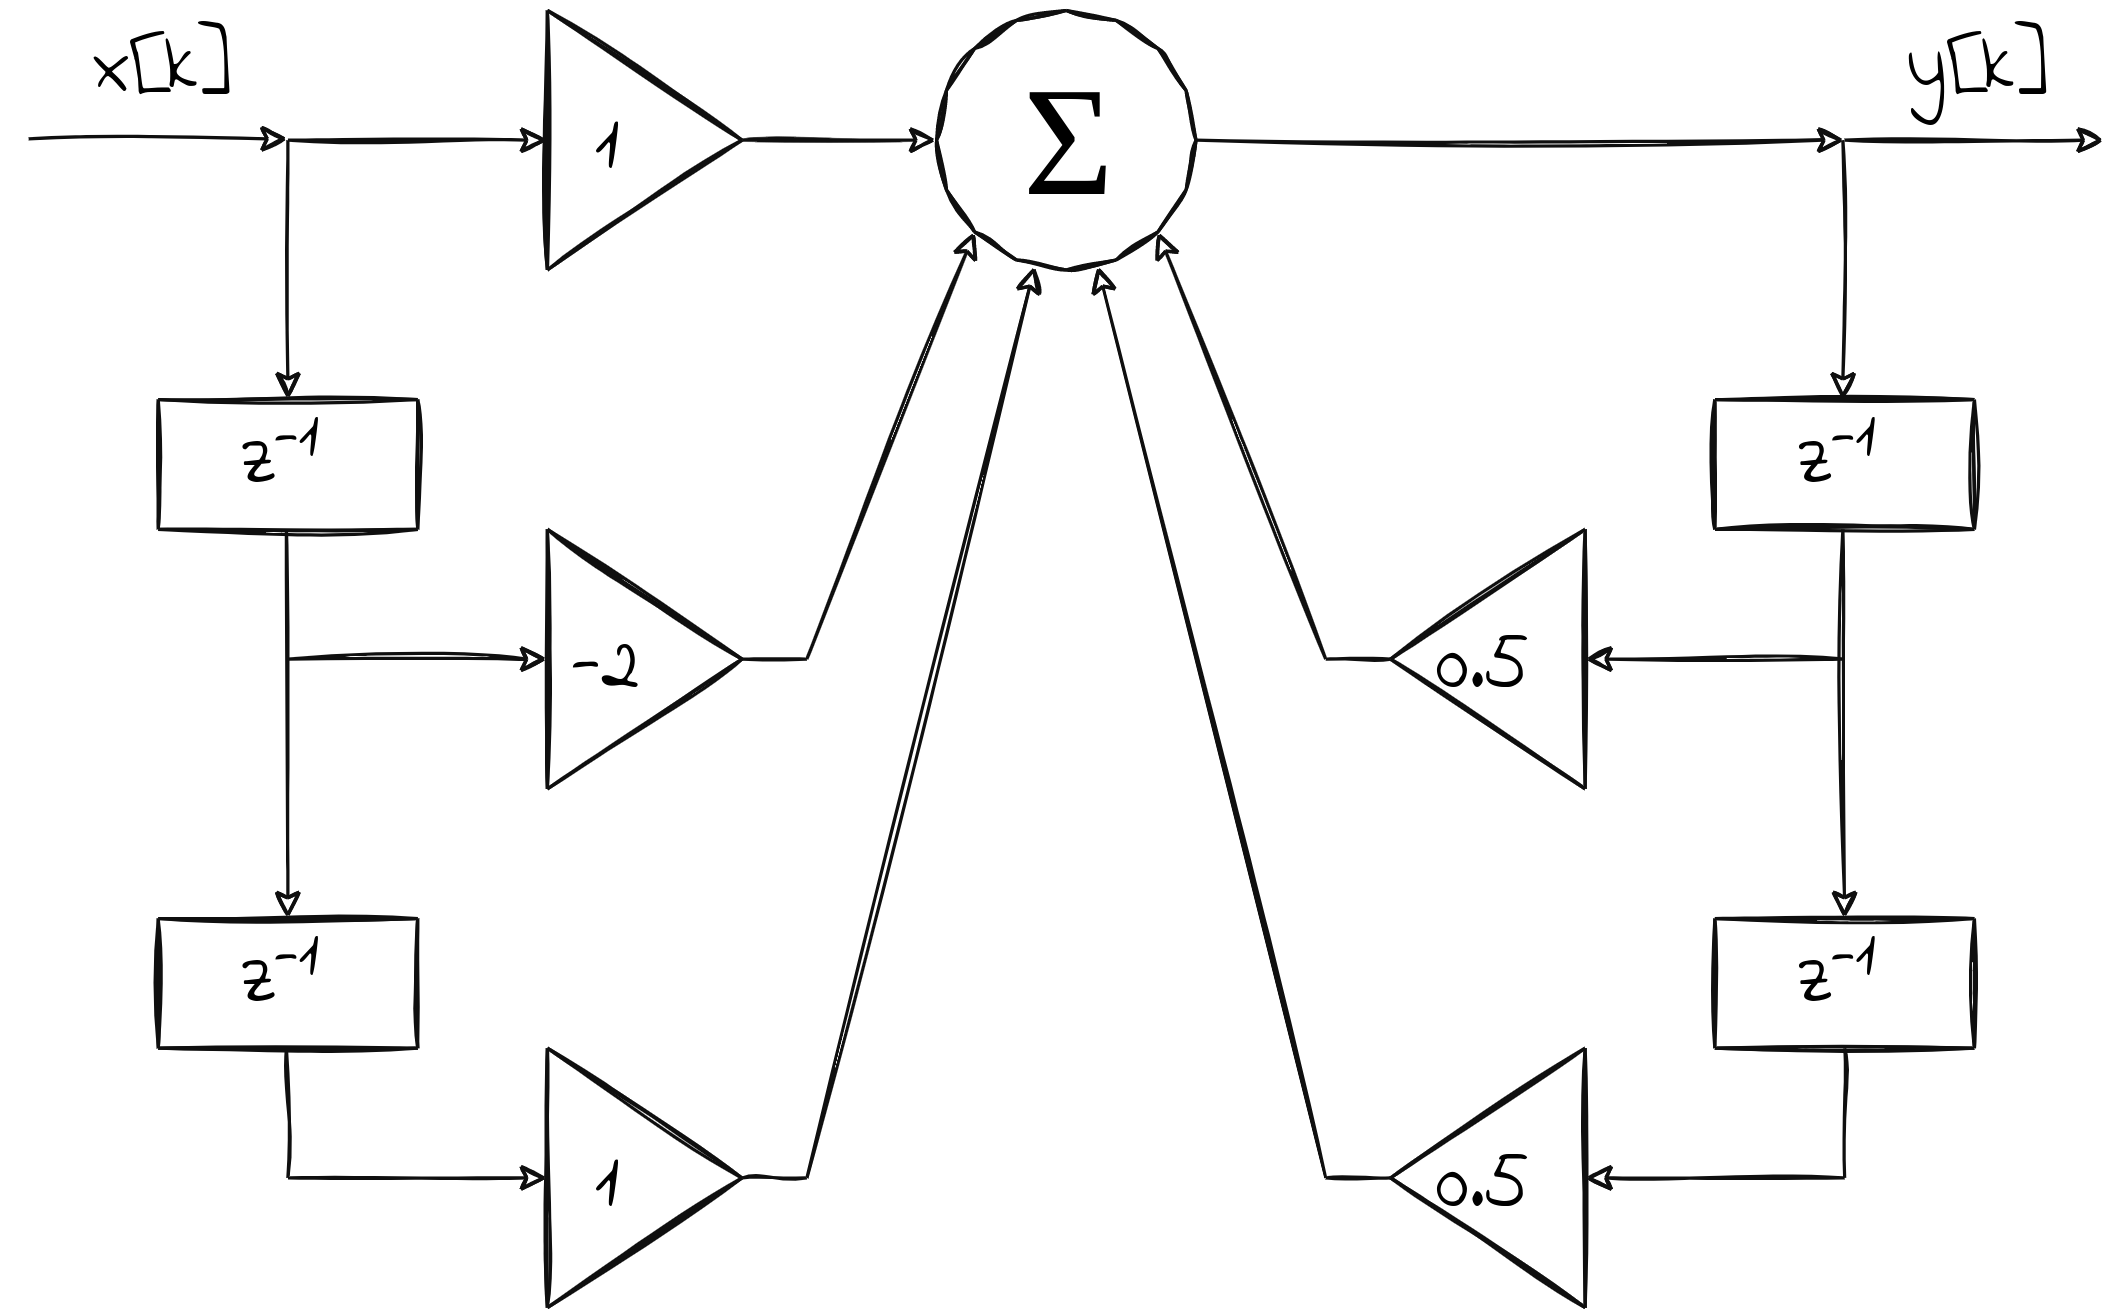
\includegraphics[width=0.6\columnwidth]{pics/fall/10/10-1.png}
	\caption{Прямая форма фильтра.}
	\label{fig:10-1}
\end{figure}

\begin{figure}[!h]
	\centering
	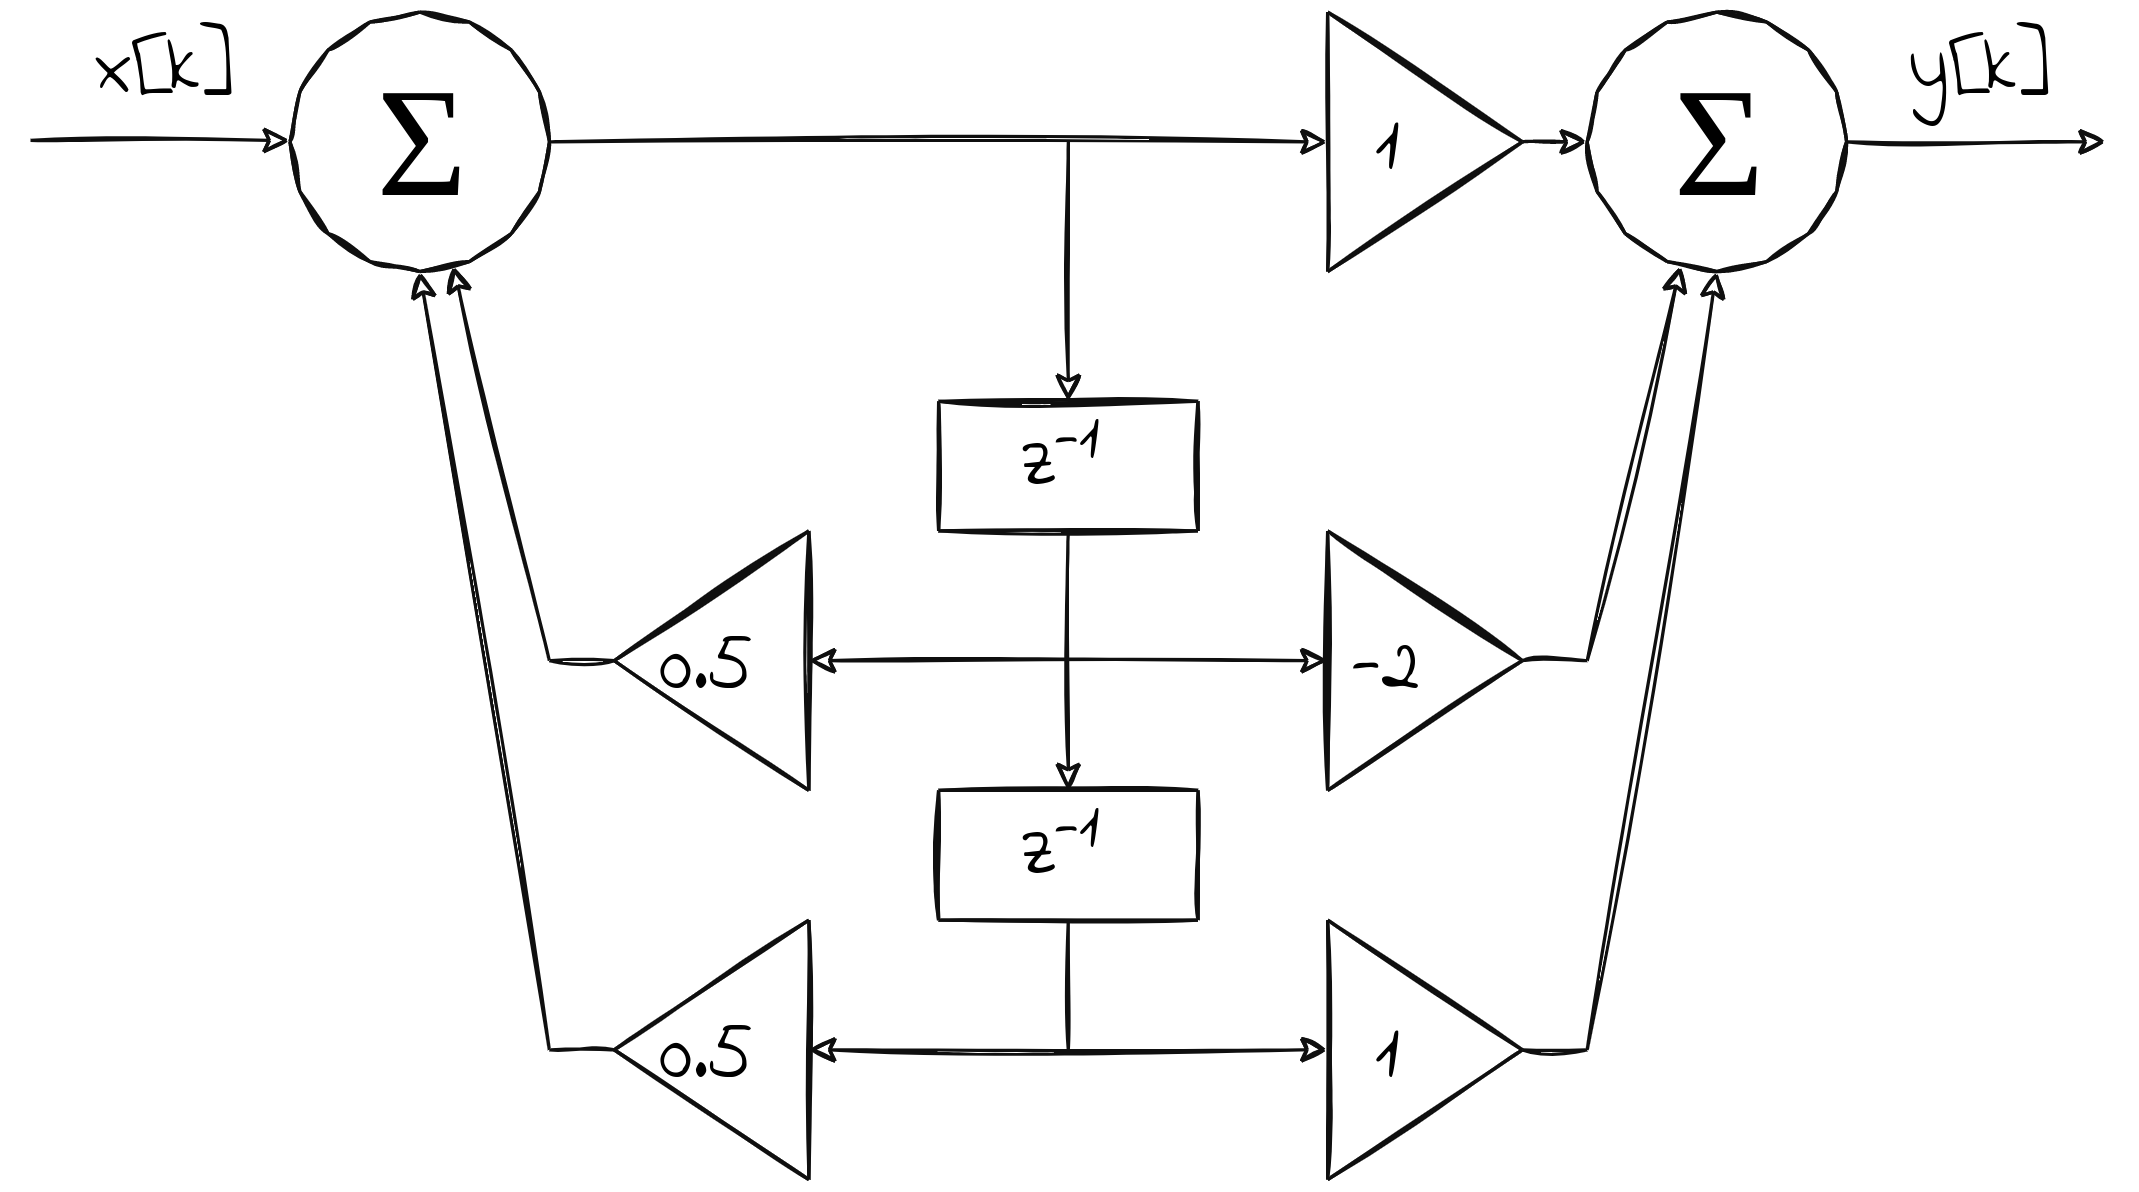
\includegraphics[width=0.6\columnwidth]{pics/fall/10/10-2.png}
	\caption{Каноническая (прямая) форма фильтра.}
	\label{fig:10-2}
\end{figure}

\footnotetext{В данном случае $\Capit{H}(z)$ содержит компенсирующие друг друга нуль и полюс. Иными словами, передаточная функция допускает упрощение. Однако схемы реализации построены для исходного вида $\Capit{H}(z)$, так как после сокращения формально получится другая передаточная функция.}

\newpage 
\section{}
Изобразить блок-схему одной из возможных реализаций фильтра с передаточной функцией

\begin{equation*}
	\Capit{H}(z) = \dfrac{0.5477 + 0.9322z^{-1} + 0.5466z^{-2}}
	{1 - 0.6106z^{-1} + 0.3029z^{-2}} \cdot
	\dfrac{0.1906 + 0.1689z^{-1} + 0.1906z^{-2}}
	{1 - 0.0013z^{-1} + 0.8093z^{-2}}
\end{equation*}

в виде каскада двух биквадратных блоков. Для биквадратных блоков выбрать прямую каноническую форму реализации.

\begin{figure}[!h]
	\centering
	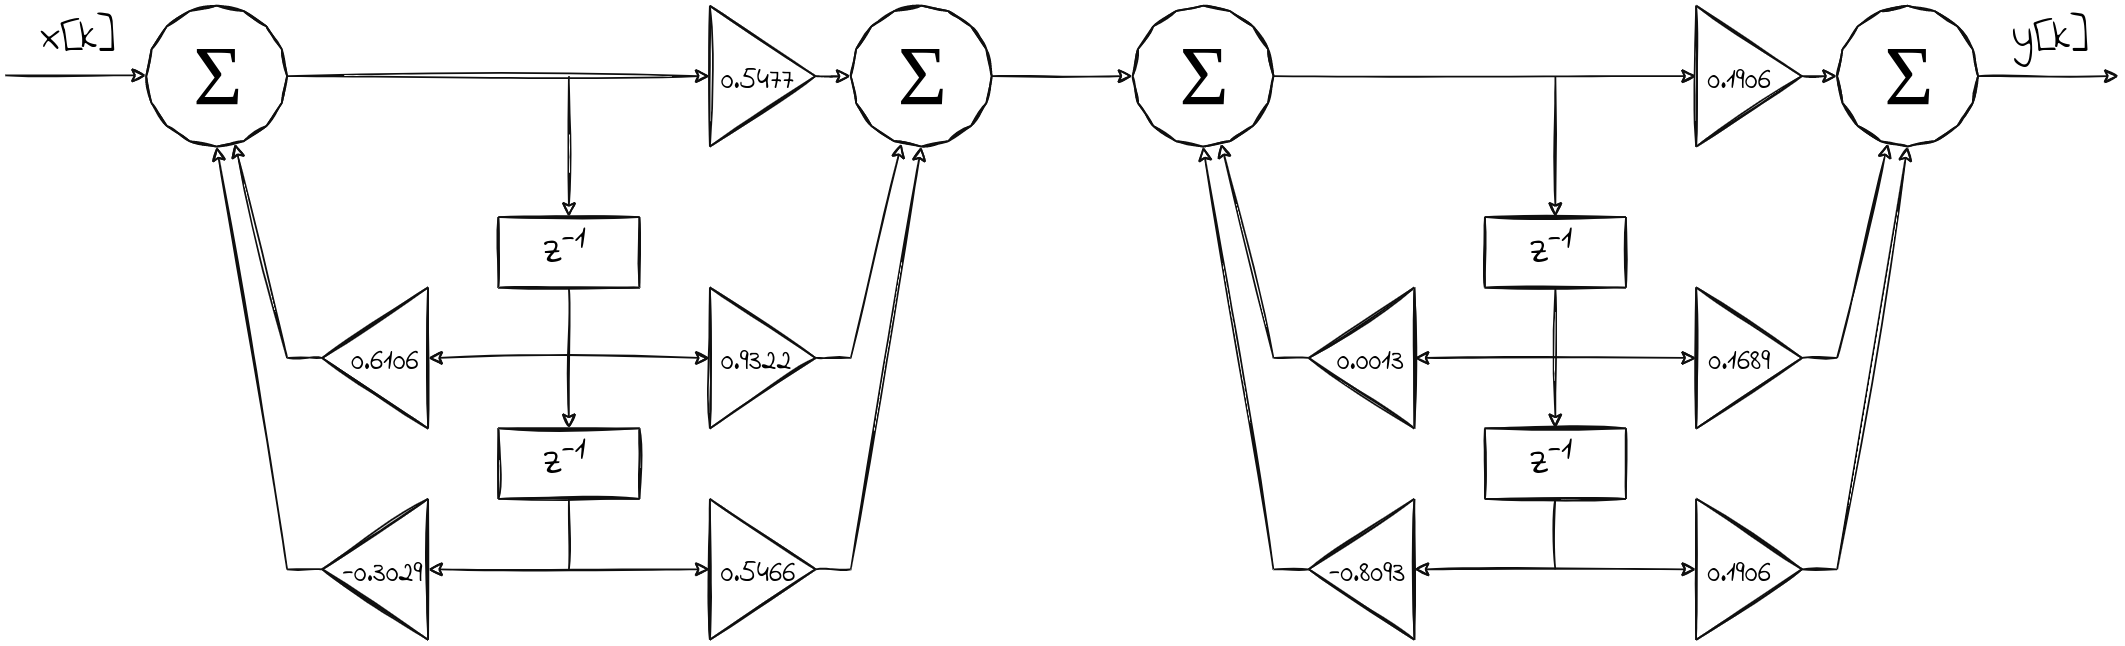
\includegraphics[width=1.0\columnwidth]{pics/fall/10/10-3.png}
	%\caption{Каноническая (прямая) форма фильтра.}
	\label{fig:10-3}
\end{figure}


\section{}
Изобразить в прямой форме блок-схему реализации цифрового фильтра второго порядка, у передаточной функции которого два комплексно-сопряжённых нуля $z_{1, 2} = \pm 0.5j$ и два комплексно-сопряжённых полюса $z_{3,4} = \pm 0.2j$, а значение частотной характеристики на частоте $0$ равно $1.28$.

\begin{align*}
	&\Capit{H}(z) = \s{k}\dfrac{(z - z_1)(z - z_2)}{(z - z_3)(z - z_4)} = \s{k}\dfrac{(z - z_1)(z - z_1^*)}{(z - z_3)(z - z_3^*)} = \s{k} \dfrac{z^2 + |z_1|^2}{z^2 + |z_3|^2} = \s{k}\dfrac{1 + |z_1|^2z^{-2}}{1 + |z_3|^2z^{-2}} = \s{k}\dfrac{1 + 0.25\cdot z^{-2}}{1 + 0.04\cdot z^{-2}}.\\
	&\Capit{H}(z)\big|_{\nu = 0} = \Capit{H}(z)\big|_{z = 1} = \s{k} \dfrac{1 + 0.25}{1 + 0.04} =
	\s{k} \cdot 1.2019 = 1.28,\quad \Rightarrow \s{k} = 1.0650.
\end{align*}

\begin{equation*}
	\Capit{H}(z) =  1.0650 \cdot \dfrac{1 + 0.25\cdot z^{-2}}{1 + 0.04\cdot z^{-2}}.
\end{equation*}

\begin{figure}[!h]
	\centering
	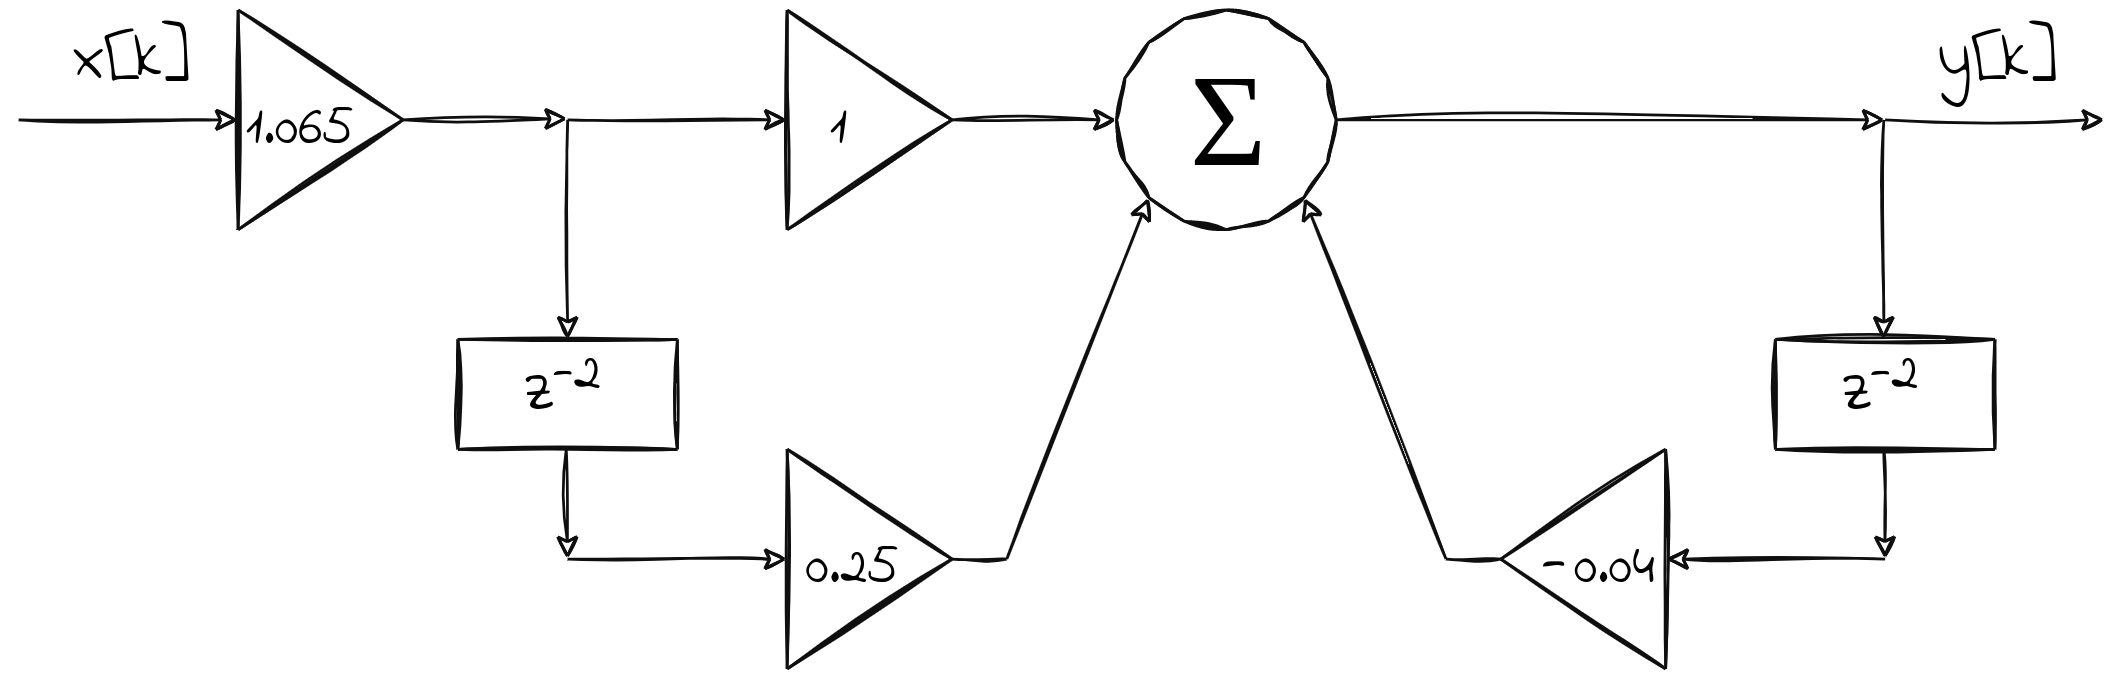
\includegraphics[width=1.0\columnwidth]{pics/fall/10/10-4.png}
	\label{fig:10-4}
\end{figure}

\section{}
Описать переход от прямой формы реализации биквадратного блока к форме, представленной ниже.

\begin{figure}[!h]
	\centering
	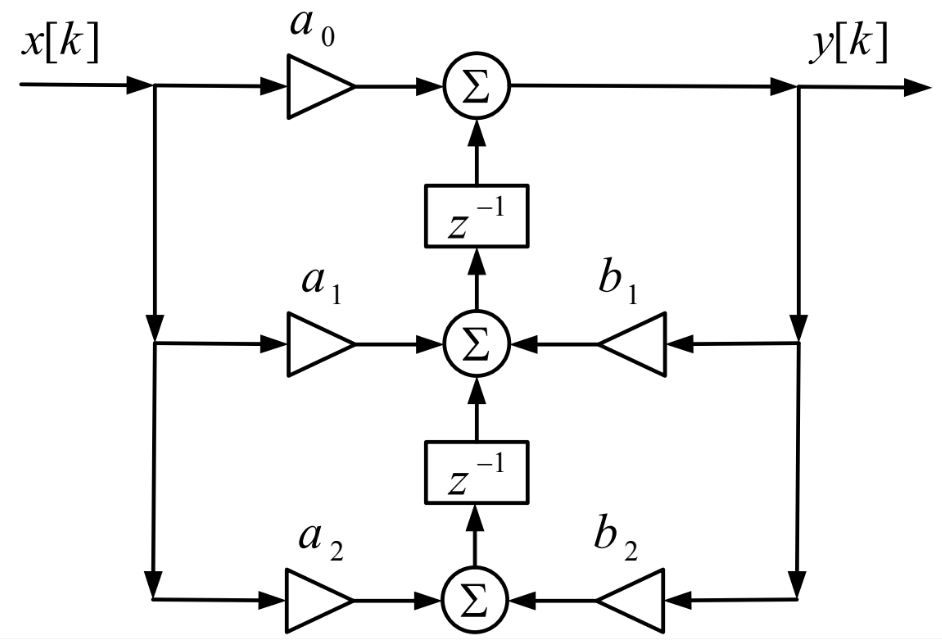
\includegraphics[width=0.6\columnwidth]{pics/fall/10/10-5.png}
	\label{fig:10-5}
\end{figure}

Чтобы получить представленную форму реализации биквадратного блока, необходимо:

\begin{itemize}
	\item поменять в прямой форме реализации последовательность вычисления операций умножения и задержки, используя в каждой ветви отдельную линию задержки на нужное количество тактов; 
	\item разделить общий единый сумматор на несколько двухвходовых сумматоров;
	\item при этом, рассмотрев любую пару соседних сумматоров, можно заметить, что
	суммируемые ими сигналы претерпевают некоторую общую задержку. Это дает возможность поменять местами операции суммирования и задержки.
	
\end{itemize}



\setcounter{chapter}{11}
\setcounter{section}{0}
%\chapter*{Неделя 11}
\protect\thispagestyle{fancy}
\section{}
Методом инвариантной импульсной характеристики получить цифровой аналог каскада из двух RC-цепочек интегрирующего типа. Записать разностное уравнение, передаточную функцию и построить блок-схему одной из реализаций получившегося фильтра.

\begin{figure}[!h]
	\centering
	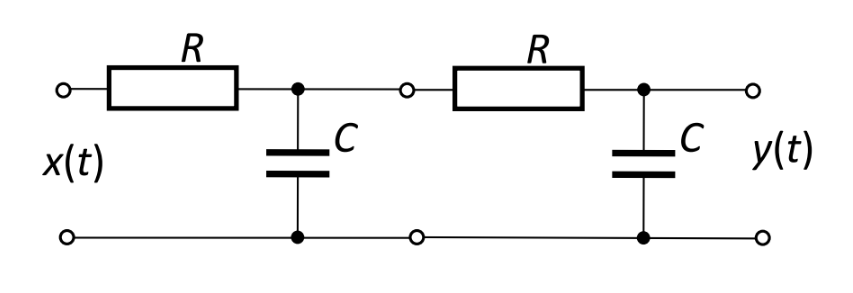
\includegraphics[width=0.55\columnwidth]{pics/fall/11/11-01.png}
	\label{fig:11-01}
\end{figure}

Уравнение для одной интегрирующей RC-цепочки:
\begin{equation*}
	RC \dfrac{dy}{dt} + y(t) = x(t).
\end{equation*}

В случае $y(0) = 0$ преобразование Лапласа принимает вид:
\begin{equation*}
	RC p \Capit{Y}(p) + \Capit{Y}(p) = \Capit{X}(p).
\end{equation*}

Передаточная функции одной RC-цепочки и каскада из двух RC-цепочек соответственно:
\begin{equation*}
	\Capit{H}_1(p) = \dfrac{\Capit{Y}(p)}{\Capit{X}(p)} = \dfrac{1}{1 + RCp},\quad
	\Capit{H}_2(p) = \big(\Capit{H}_1(p)\big)^2 = \dfrac{1}{\left(1 + RCp\right)^2}.
\end{equation*}

Вычислим обратное преобразование Лапласа:
\begin{align*}
	h_a(t) &= \dfrac{1}{2 \pi j} \oint \limits_{\gamma} \Capit{H}_2(p) e^{pt} dp = 
	\dfrac{1}{2 \pi j} \oint \limits_{\gamma} \dfrac{e^{pt} dp}{\left(1 + RCp\right)^2} = 
	\underset{p_p = -1/RC}{\text{res}} \left\{\dfrac{e^{pt}}{(1 + RCp)^2}\right\} =\\ &=
	\dfrac{1}{(RC)^2}\underset{p_p = -1/RC}{\text{res}} \left\{\dfrac{e^{pt}}{\left(p - (-\frac{1}{RC})\right)^2}\right\} =
	\dfrac{1}{(RC)^2} \lim \limits_{p \to -1/RC} \left\{\dfrac{de^{pt}}{dp}\right\} =
	\dfrac{t}{(RC)^2} \exp\left(-\dfrac{t}{RC}\right).
\end{align*}

Получим импульсную характеристику цифрового фильтра:
\begin{align*}
	h[k] &= \Delta t \cdot h_a(k \Delta t) = \dfrac{k (\Delta t)^2}{(RC)^2} \exp\left(-\dfrac{k \Delta t}{RC}\right).
\end{align*}

Наконец, передаточная функция искомого цифрового фильтра:
\begin{align*}
	\Capit{H}(z) &= \sum \limits_{k=0}^{+\infty}h[k]z^{-k} = \sum \limits_{k=0}^{+\infty} \dfrac{k \Delta t^2}{(RC)^2} \exp\left(-\dfrac{k \Delta t}{RC}\right) z^{-k} = \left(\dfrac{\Delta t}{RC}\right)^2 \sum \limits_{k=0}^{+\infty} k
	\left(\exp\left(-\dfrac{\Delta t}{RC}\right) z^{-1} \right)^k = \\ &=
	\left(\dfrac{\Delta t}{RC}\right)^2 \sum \limits_{k=0}^{+\infty} k \alpha^k = 
	\left(\dfrac{\Delta t}{RC}\right)^2 \dfrac{d}{d\alpha} \left\{ \sum \limits_{k=0}^{+\infty} \alpha^k \right\} =
	\left(\dfrac{\Delta t}{RC}\right)^2 \dfrac{d}{d\alpha} \left\{\dfrac{1}{1 - \alpha} \right\} =
	\left(\dfrac{\Delta t}{RC}\right)^2 \dfrac{\alpha}{(1 - \alpha)^2} = \\ &=
	\left(\dfrac{\Delta t}{RC}\right)^2 \dfrac{\exp\left(-\dfrac{\Delta t}{RC}\right) z^{-1} }{\left(1 - \exp\left(-\dfrac{\Delta t}{RC}\right) z^{-1} \right)^2} =
	\dfrac{\left(\dfrac{\Delta t}{RC}\right)^2 \exp\left(-\dfrac{\Delta t}{RC}\right) z^{-1}}{1 - 2\exp\left(-\dfrac{\Delta t}{RC}\right) z^{-1} + \exp\left(-\dfrac{2\Delta t}{RC}\right) z^{-2}}, \quad \Big|\exp\left(-\dfrac{\Delta t}{RC}\right) z^{-1}\Big| < 1.
\end{align*}

Разностное уравнение принимает вид:
\begin{align*}
	\left(\dfrac{\Delta t}{RC}\right)^2 \exp\left(-\dfrac{\Delta t}{RC}\right) x[k-1] = y[k] - 2\exp\left(-\dfrac{\Delta t}{RC}\right) y[k-1] + \exp\left(-\dfrac{2\Delta t}{RC}\right) y[k-2],\quad y[-2] = y[-1] = 0.
\end{align*}

\begin{figure}[!h]
	\centering
	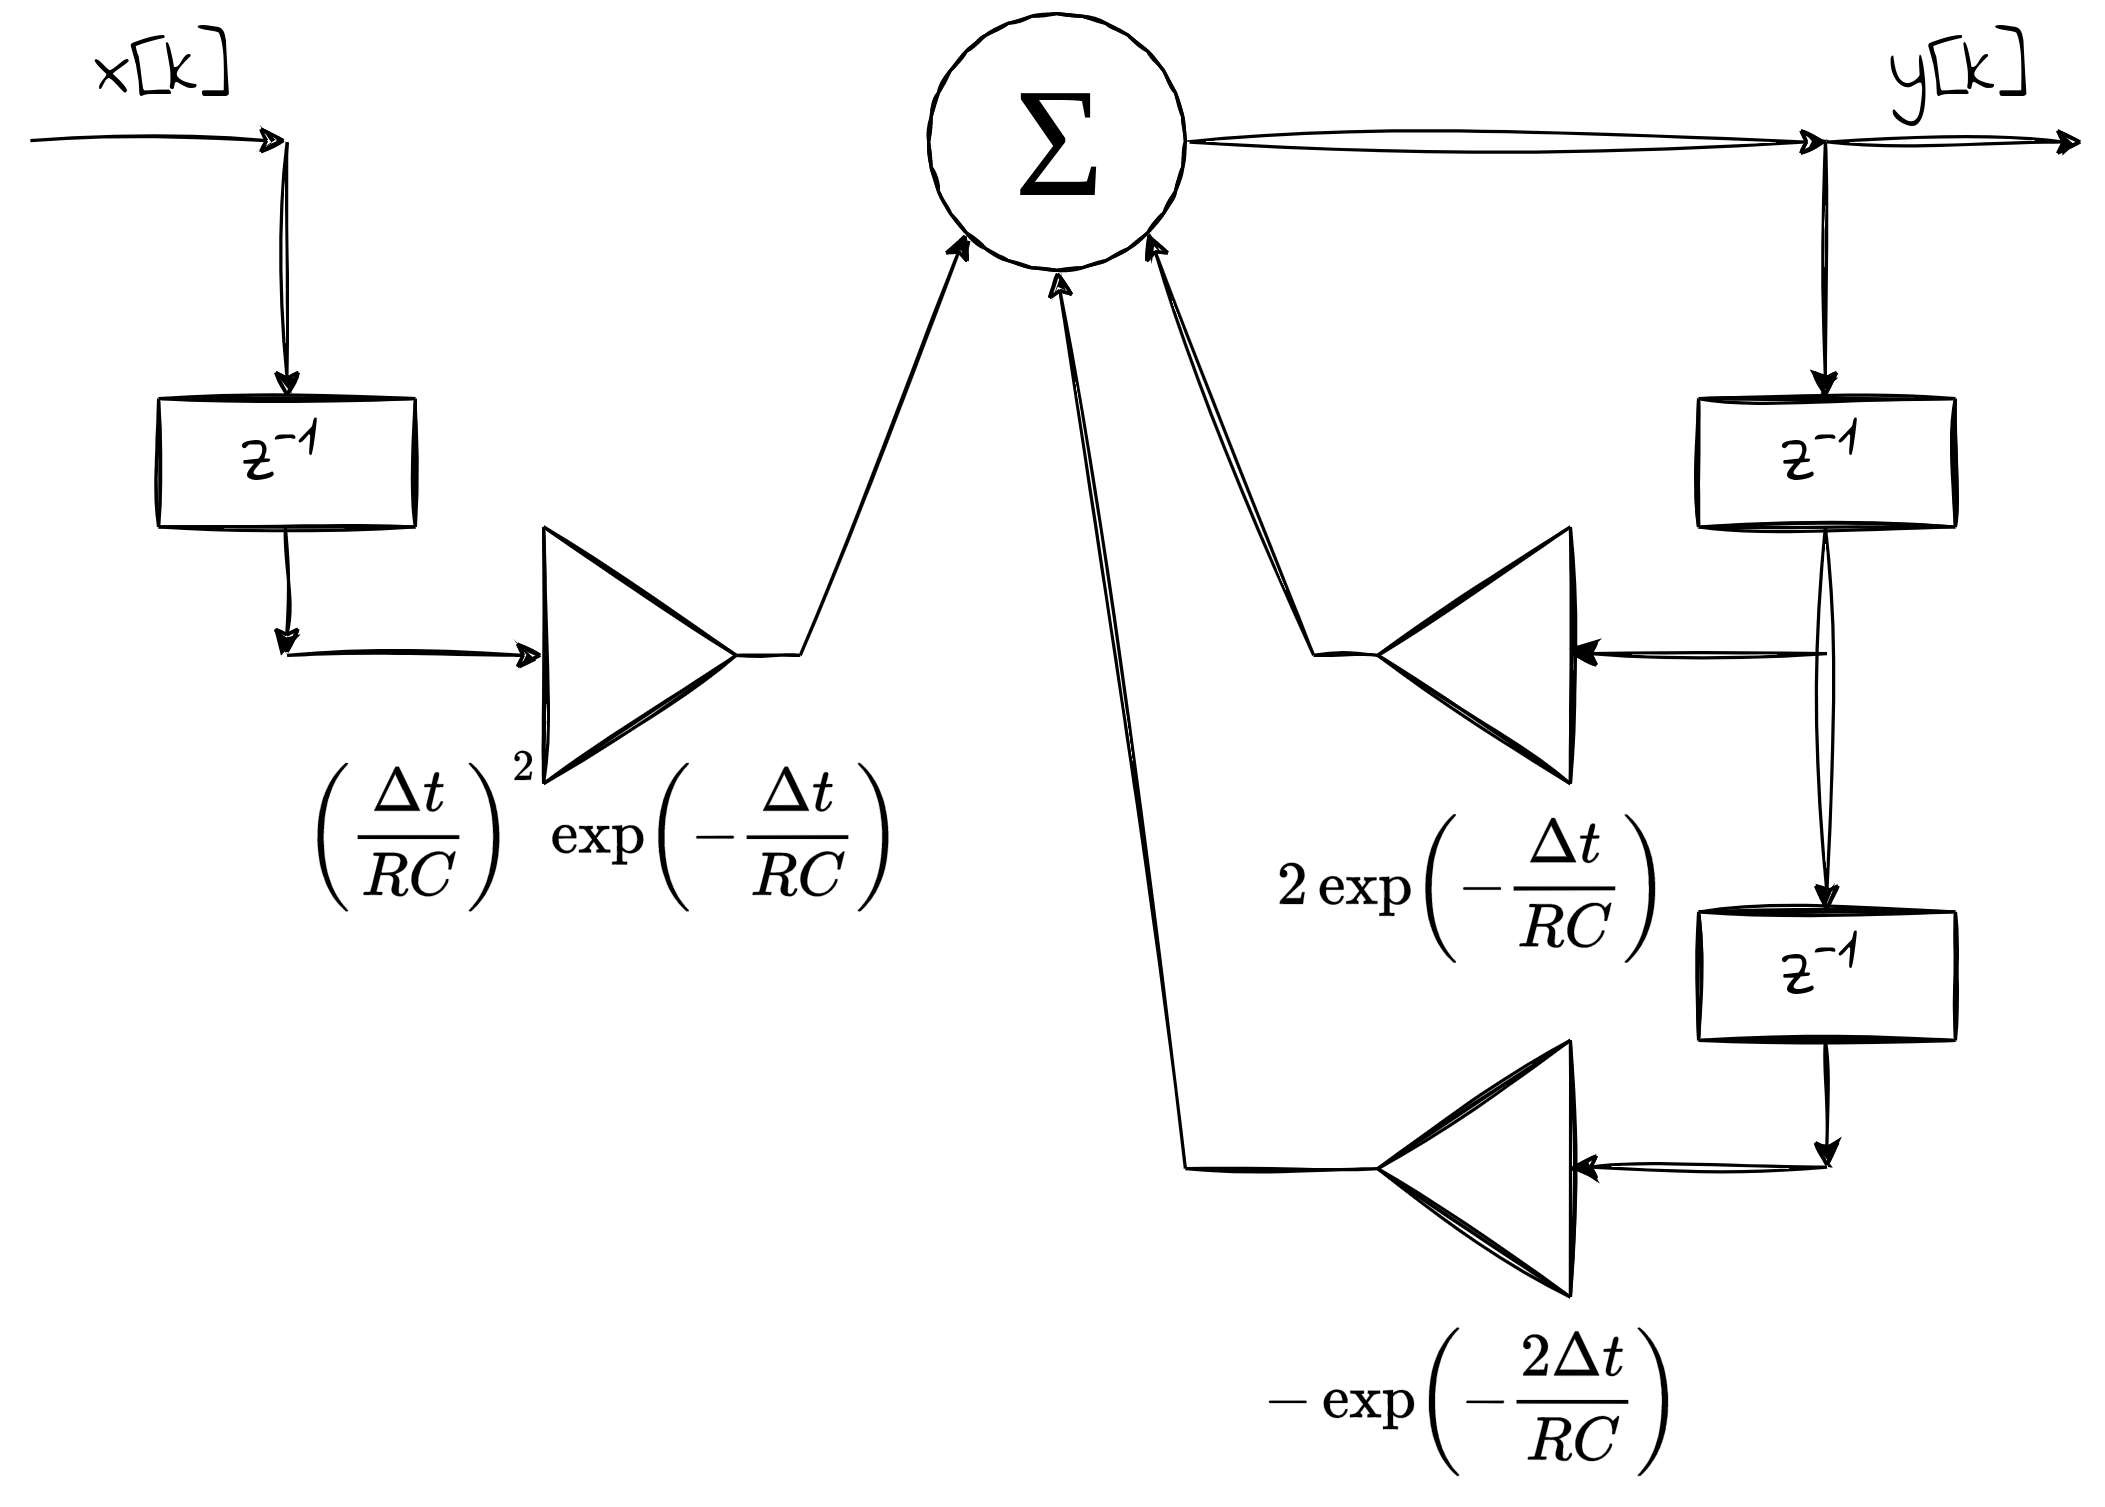
\includegraphics[width=0.75\columnwidth]{pics/fall/11/11-1.png}
	\label{fig:11-1}
\end{figure}

\newpage
\section{}
Методом билинейного $\Capit{Z}$-преобразования получить цифровой аналог RC-цепочки интегрирующего типа. Записать разностное уравнение, передаточную функцию, изобразить нуль-полюсную диаграмму и построить блок-схему одной из реализаций получившегося фильтра.

\begin{figure}[!h]
	\centering
	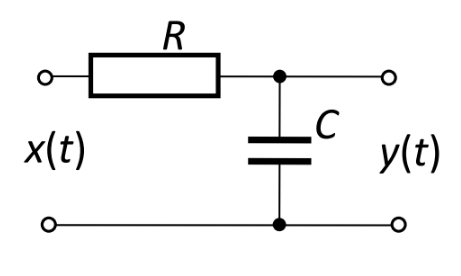
\includegraphics[width=0.35\columnwidth]{pics/fall/11/11-02.png}
	\label{fig:11-02}
\end{figure}

Уравнение для одной интегрирующей RC-цепочки:
\begin{equation*}
	RC \dfrac{dy}{dt} + y(t) = x(t).
\end{equation*}

В случае $y(0) = 0$ преобразование Лапласа принимает вид:
\begin{equation*}
	RC p \Capit{Y}(p) + \Capit{Y}(p) = \Capit{X}(p).
\end{equation*}

Передаточная функции одной интегрирующей RC-цепочки:
\begin{equation*}
	\Capit{H}_1(p) = \dfrac{\Capit{Y}(p)}{\Capit{X}(p)} = \dfrac{1}{1 + RCp}.
\end{equation*}

Согласно методу билинейного $\Capit{Z}$-преобразования делаем замену $p = \dfrac{2}{\Delta t} \dfrac{1 - z^{-1}}{1 + z^{-1}}$:

\begin{align*}
	\Capit{H}(z) = \dfrac{1}{1 + RC \dfrac{2}{\Delta t} \dfrac{1 - z^{-1}}{1 + z^{-1}}} = 
	\dfrac{1 + z^{-1}}{\left(1 + \dfrac{2RC}{\Delta t}\right) + \left(1 - \dfrac{2RC}{\Delta t}\right)z^{-1}} =
	\left( \dfrac{\Delta t}{\Delta t + 2RC}\right) \dfrac{1 + z^{-1}}{1 + \dfrac{\Delta t - 2RC}{\Delta t + 2RC}z^{-1}}.
\end{align*}


\begin{figure}[!h]
	\centering
	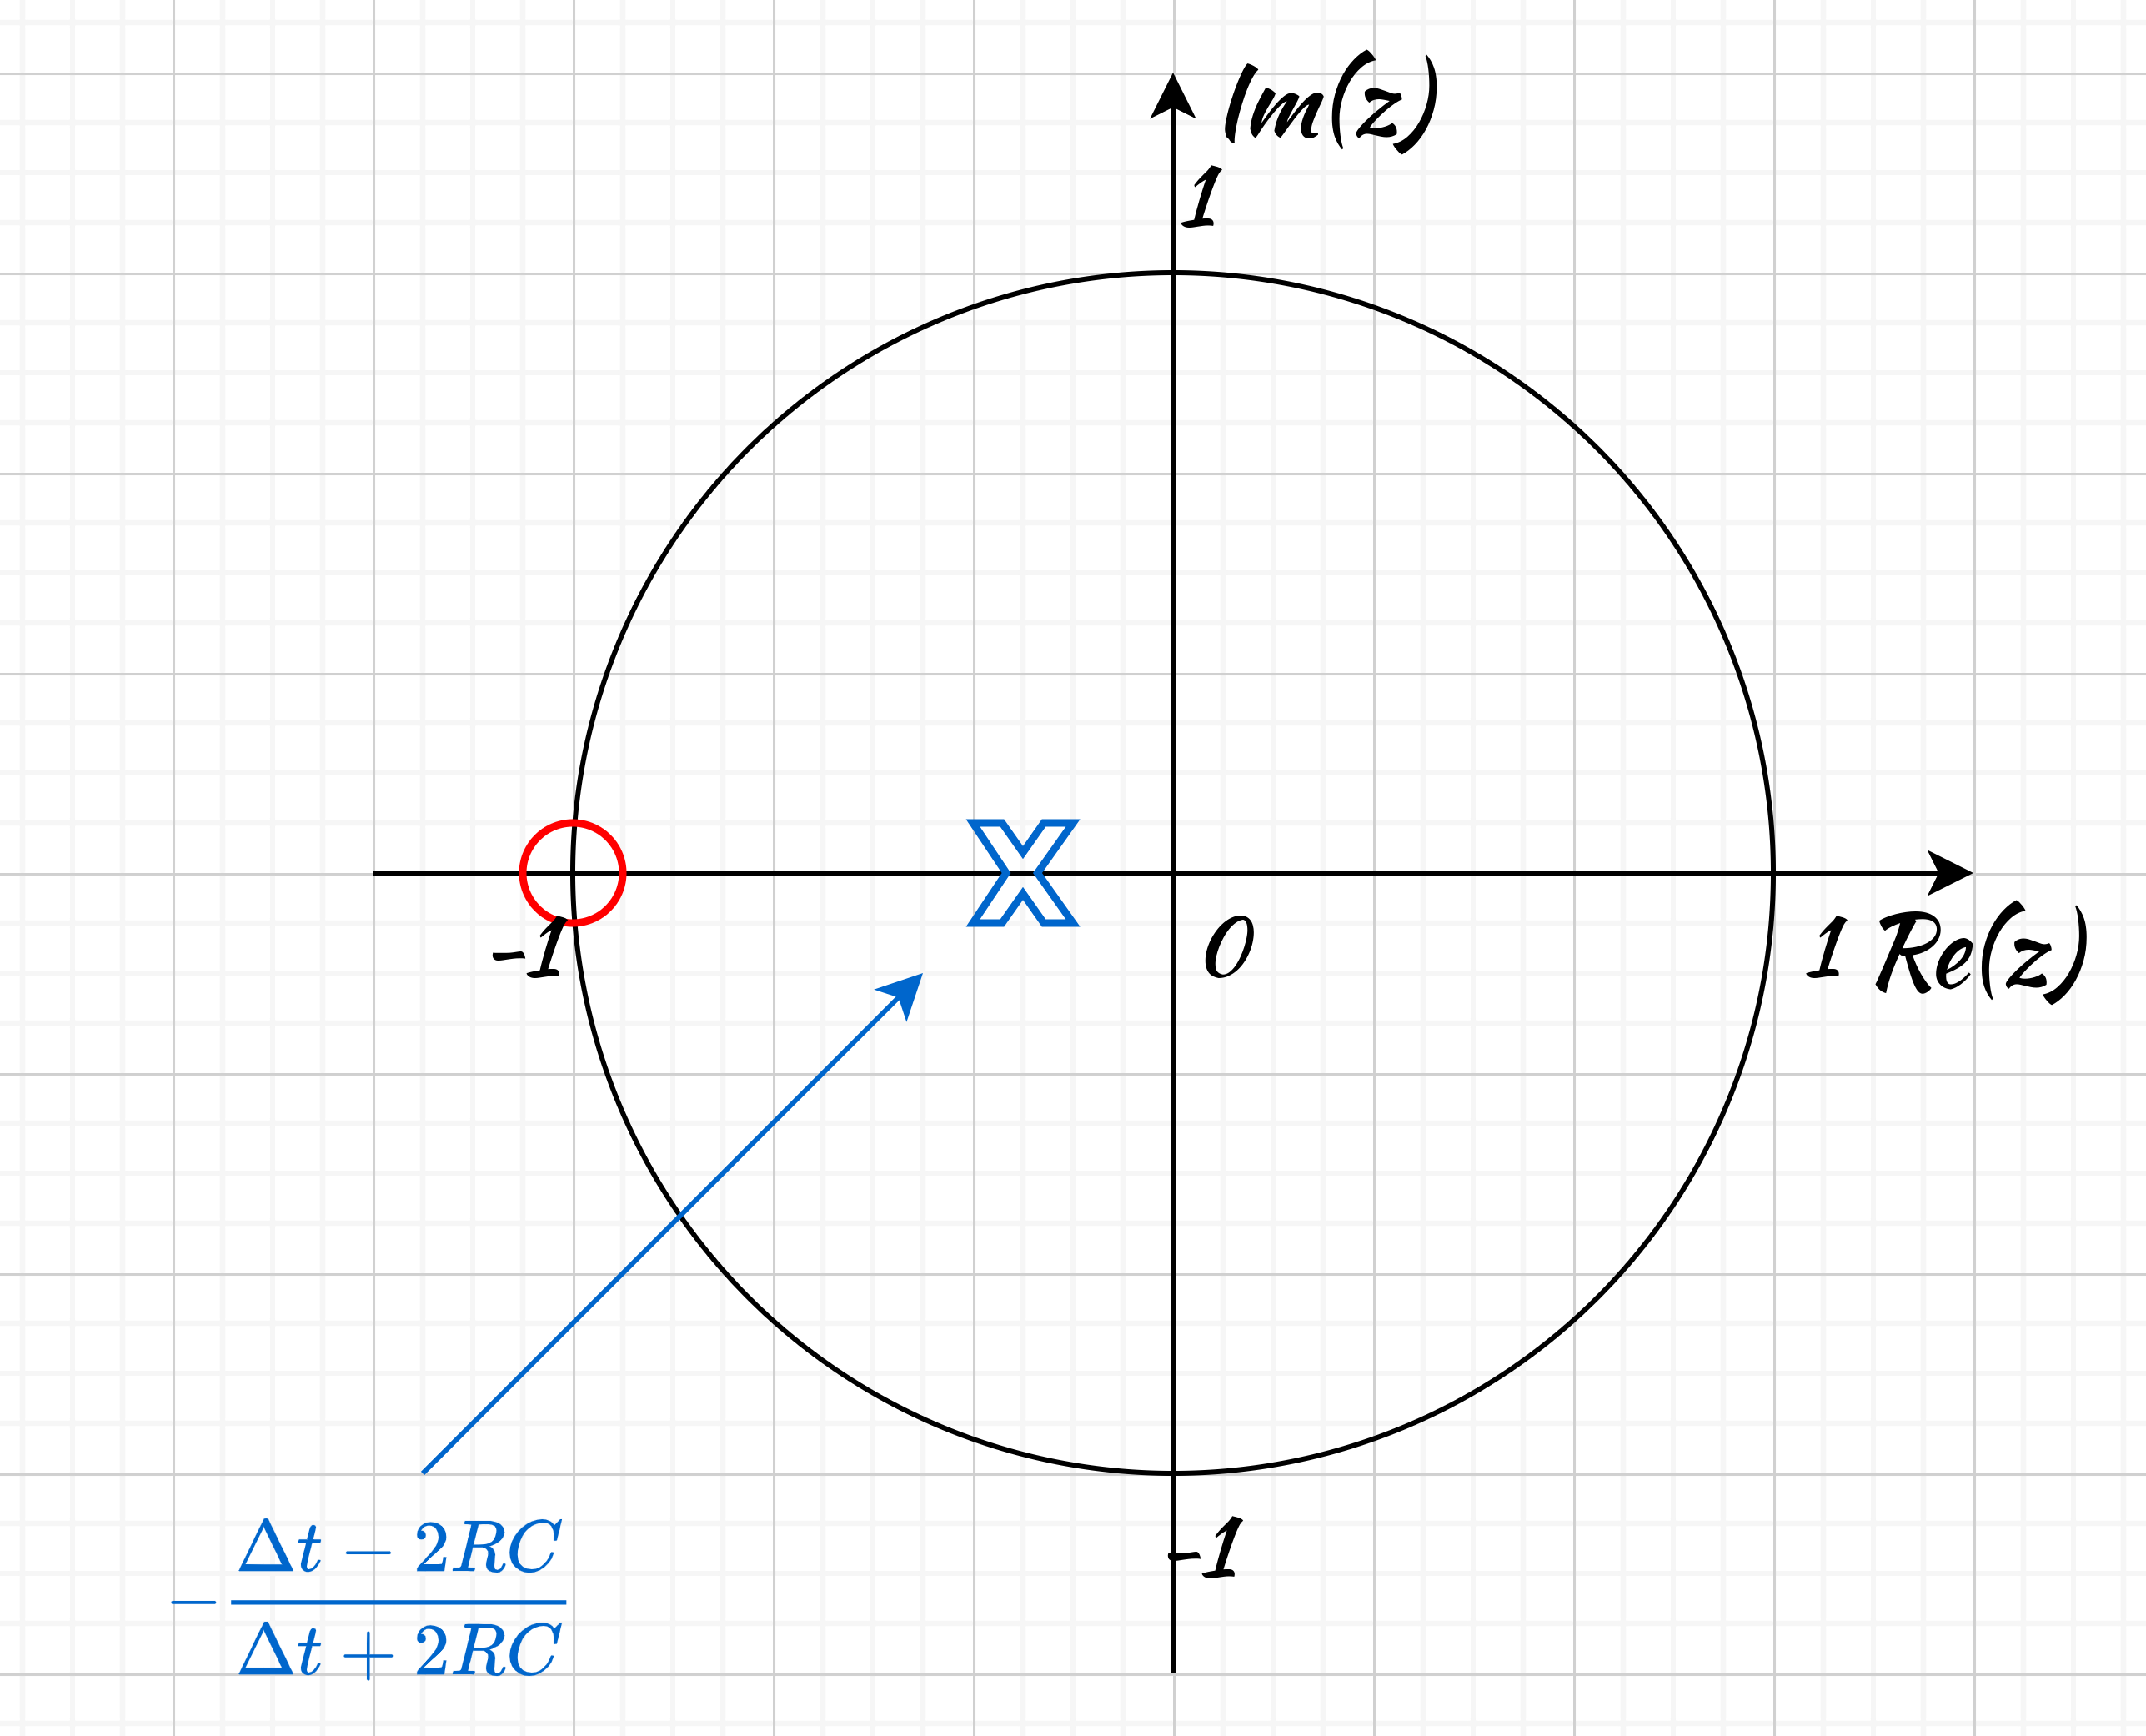
\includegraphics[width=0.55\columnwidth]{pics/fall/11/11-3.png}
	\label{fig:11-3}
\end{figure}

Разностное уравнение принимает вид:
\begin{align*}
	\left( \dfrac{\Delta t}{\Delta t + 2RC}\right) \big(x[k] + x[k-1]\big) = y[k] + \left( \dfrac{\Delta t - 2RC}{\Delta t + 2RC}\right) y[k-1], \quad y[-1] = 0.
\end{align*}


\begin{figure}[!h]
	\centering
	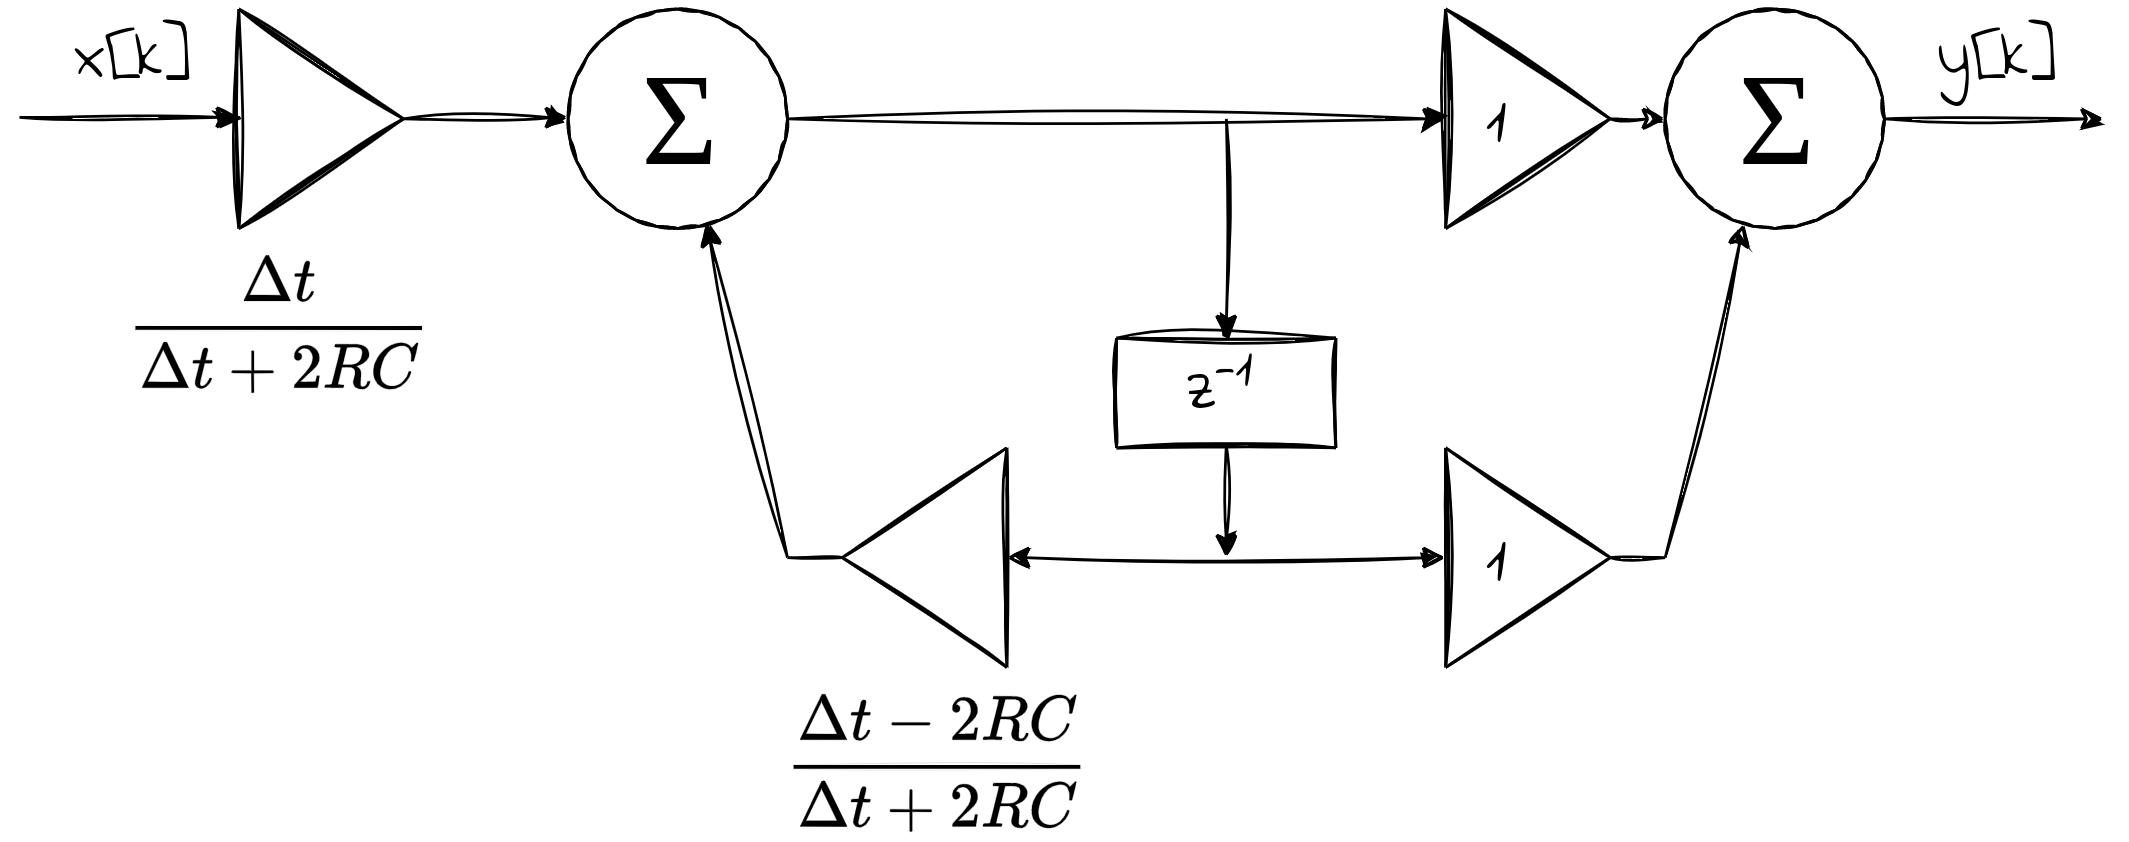
\includegraphics[width=0.75\columnwidth]{pics/fall/11/11-2.png}
	\label{fig:11-2}
\end{figure}


\newpage
\section{}
Получить выражения для частотной характеристики, АЧХ и ФЧХ фильтра, заданного разностным уравнением

\begin{equation*}
	y[k] = (1 - \Capit{A})x[k] + \Capit{A}\cdot y[k-1],\quad y[-1] = 0,
\end{equation*}
где $0 < \Capit{A} < 1$ (квазиинтегратор).



\begin{equation*}
	\Capit{H}(z) = \dfrac{\Capit{Y}(z)}{\Capit{X}(z)} = \dfrac{1 - \Capit{A}}{1 - \Capit{A}z^{-1}}
\end{equation*}

\begin{equation*}
	\Capit{H}(\nu) = \Capit{H}(z)\big|_{z = \exp(j 2\pi \nu)} = \dfrac{1 - \Capit{A}}{1 - \Capit{A}\exp(-j 2\pi \nu)} =
	\dfrac{1 - \Capit{A}}{(1 - \Capit{A}\cos(2\pi \nu)) + j \Capit{A} \sin(2\pi \nu)}.
\end{equation*}

\begin{align*}
	|\Capit{H}(\nu)| &= \dfrac{1 - \Capit{A}}{\sqrt{(1 - \Capit{A}\cos(2\pi \nu))^2 + \Capit{A}^2 \sin^2(2\pi \nu)}} = \dfrac{1 - \Capit{A}}{\sqrt{1  + \Capit{A}^2- 2\Capit{A}\cos(2\pi \nu)}}.\\
	\arg\{\Capit{H}(\nu)\} &= - \arg \{(1 - \Capit{A}\cos(2\pi \nu)) + j \Capit{A} \sin(2\pi \nu)\} =
	-\arctg \left\{ \dfrac{\Capit{A}\sin(2\pi \nu)}{1 - \Capit{A}\cos(2\pi \nu)}\right\}.
\end{align*}


\setcounter{chapter}{12}
\setcounter{section}{0}
%\chapter*{Неделя 12}
\protect\thispagestyle{fancy}
\section{}
Пусть выходные отсчёты нерекурсивного фильтра 1-ого порядка получаются усреднением текущего и предшествующего входных отсчётов
\begin{equation*}
	y[k] = 0.5x[k] + 0.5x[k-1].
\end{equation*}

Найти импульсную характеристику $h[k]$ и переходную характеристику фильтра $g[k]$, определить время установления по переходной характеристике. Построить нуль-полюсную диаграмму и исследовать фильтр на устойчивость.

\begin{equation*}
	\Capit{H}(z) = \dfrac{\Capit{Y}(z)}{\Capit{X}(z)} = 0.5 (1 + z^{-1}) = h[0] + h[1]z^{-1}, \quad \Rightarrow h[k] = 
	\begin{cases}
		0.5, & \text{если } k = 0 \text{ или } k=1,\\
		0, & \text{иначе}.
	\end{cases}
\end{equation*}

\begin{equation*}
	g[k] = \sum \limits_{m = 0}^{+\infty} h[k + m] = 
	\begin{cases}
		0.5, & \text{если } k = 0,\\
		1, & \text{если } k \geq 1,\\
		0, & \text{иначе}.
	\end{cases}
\end{equation*}

Время установления -- $1$ такт (если считать с нулевого).

\begin{equation*}
	\Capit{H}(z) = 0.5 (1 + z^{-1}) = \dfrac{1 + z}{2z},\quad \Rightarrow
	z_{p} = 0, z_{o} = -1.
\end{equation*}

\begin{figure}[!h]
	\centering
	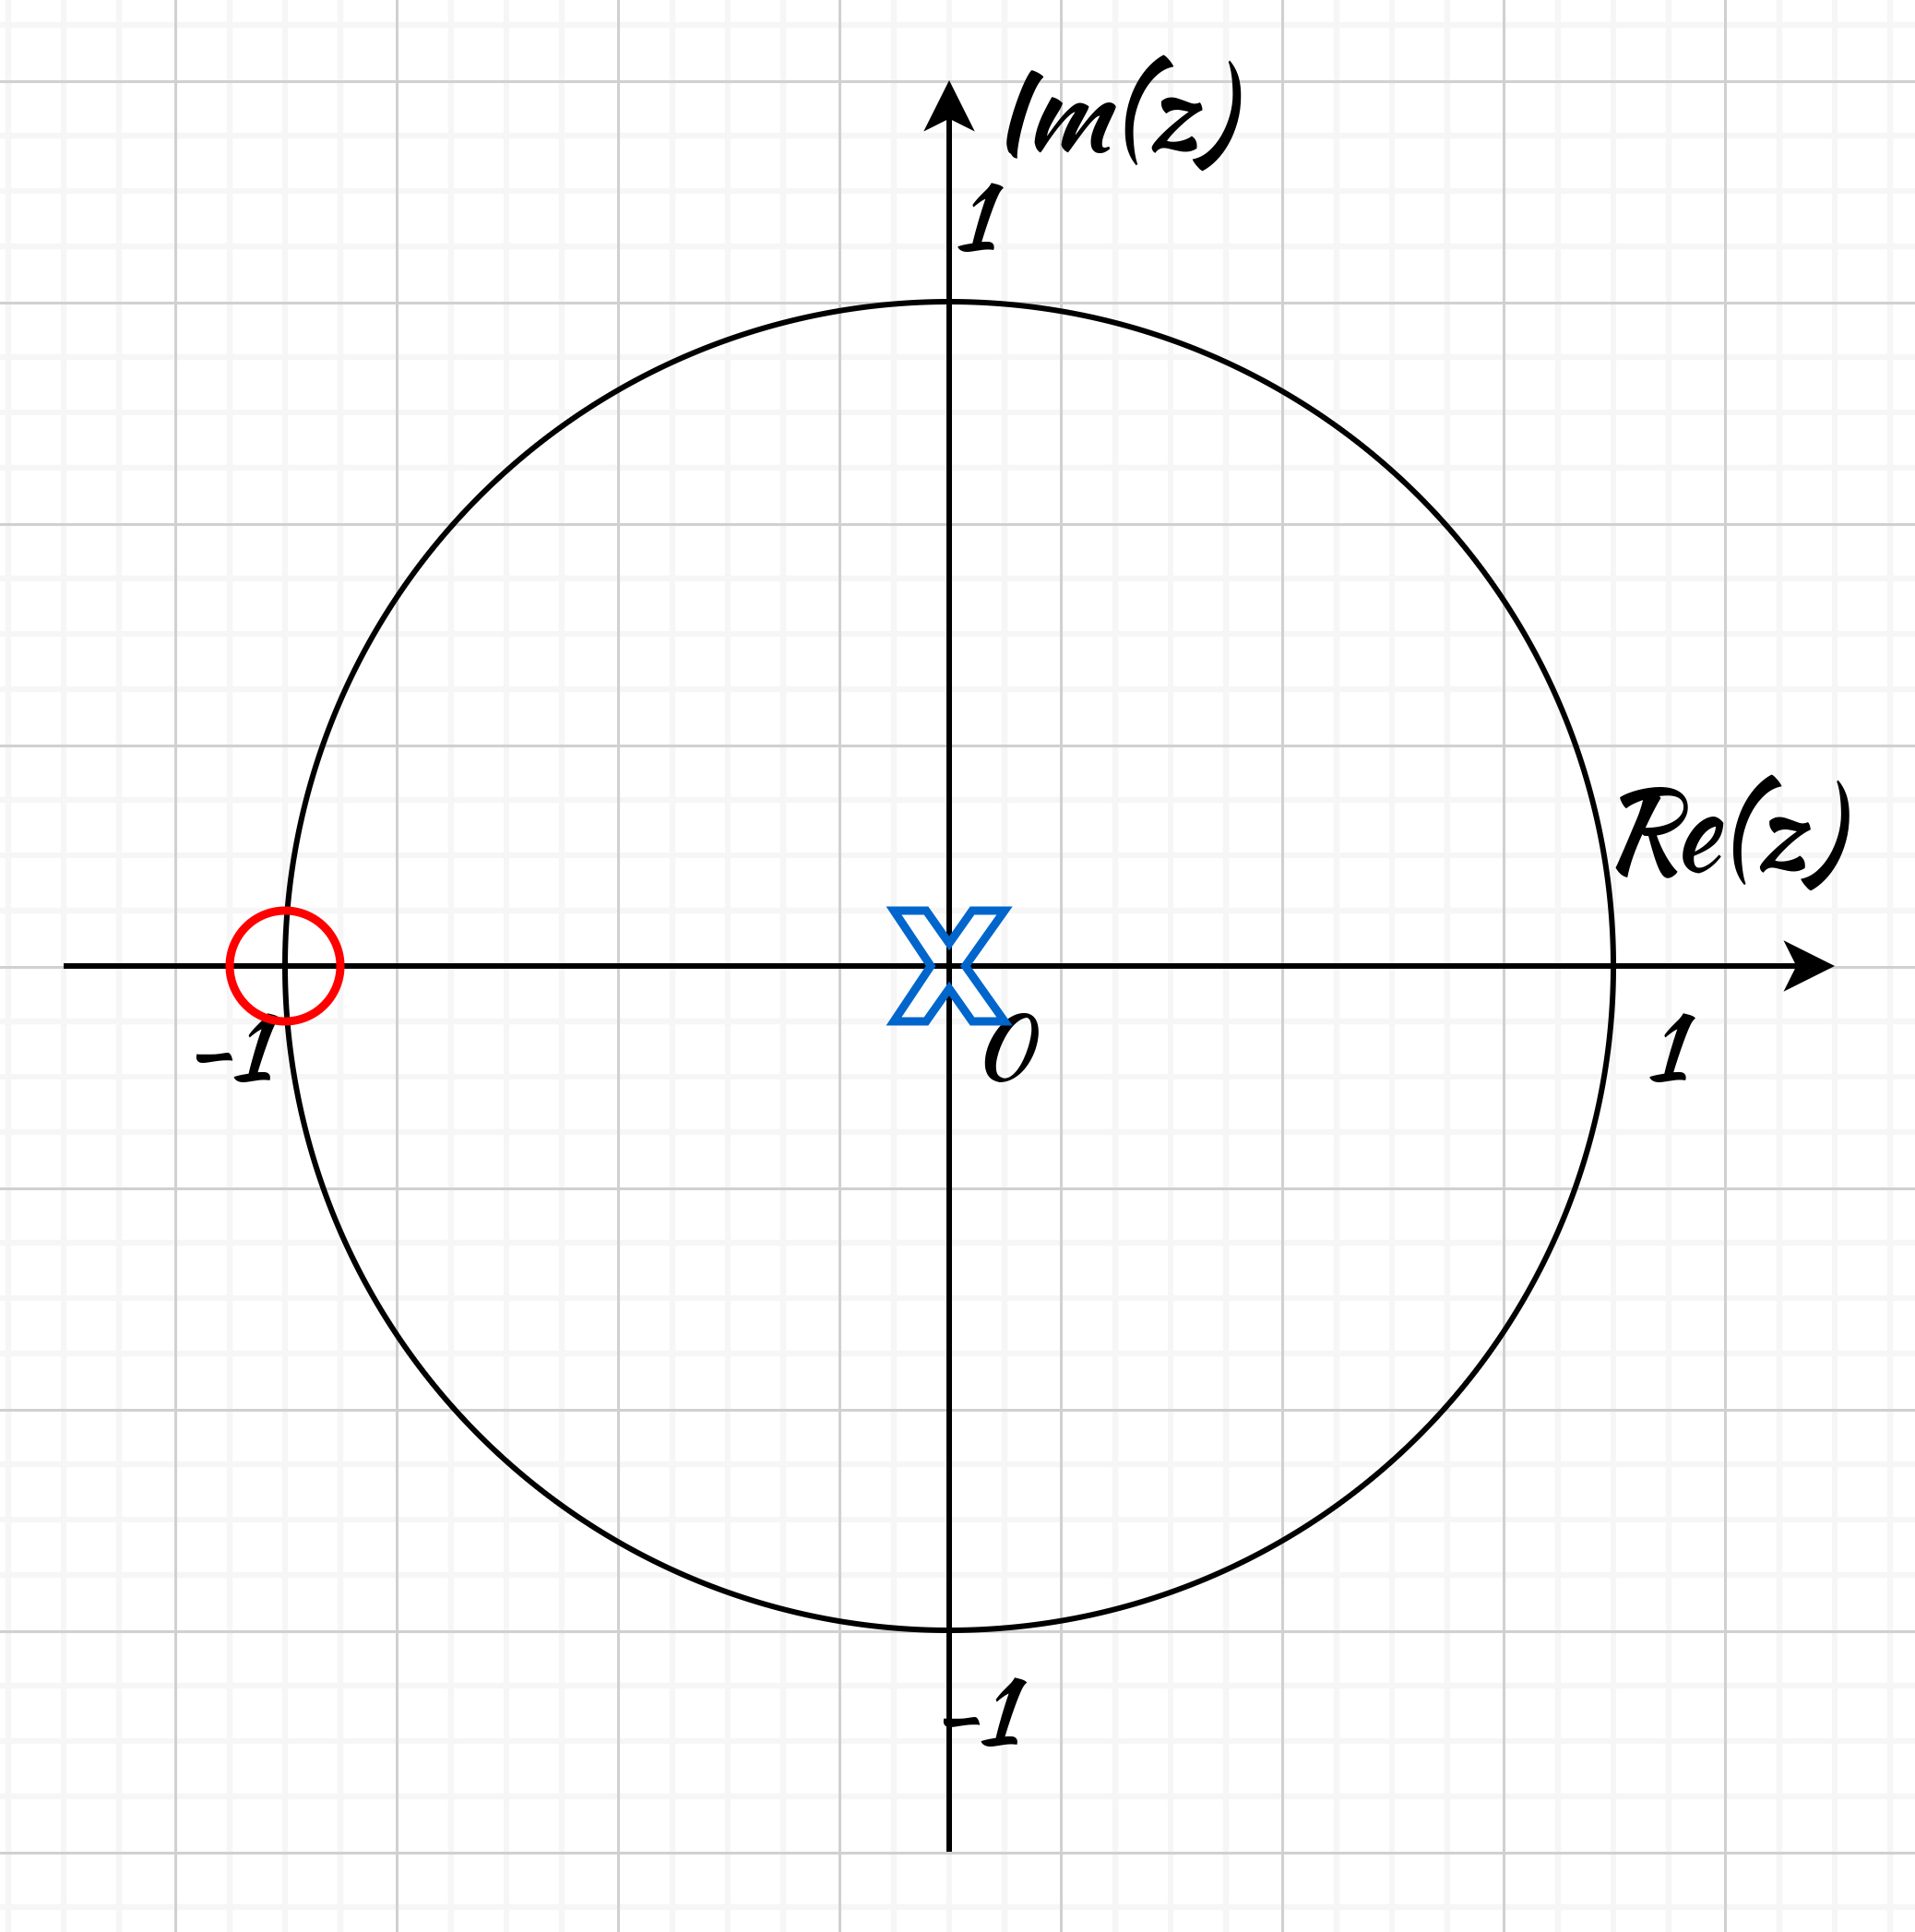
\includegraphics[width=0.4\columnwidth]{pics/fall/12/12-1-1.png}
	\label{fig:12-1-1}
\end{figure}

Единственный полюс $z_p = 0$ лежит внутри единичного круга на комплексной плоскости, то есть
система является устойчивой по входу.



\section{}
Для нерекурсивного фильтра второго порядка с передаточной функцией
\begin{equation*}
	\Capit{H}(z) = 1 - 0.1z^{-1} - 0.9z^{-2}
\end{equation*}
построить блок-схему реализации в прямой форме и в виде последовательного соединённых нерекурсивных фильтров первого порядка. Построить нуль-полюсную диаграмму и исследовать фильтр на устойчивость. Определить импульсную характеристику $h[k]$ и переходную характеристику $g[k]$ фильтра.

\begin{align*}
	\Capit{H}(z) = 1 - 0.1z^{-1} - 0.9z^{-2} = \Big(1 - z^{-1}\Big)\Big(1 + \frac{9}{10}z^{-1}\Big) =
	\dfrac{\Big(z - 1\Big)\Big(z + \dfrac{9}{10}\Big)}{z^2},\\
	z_{p} = 0,\; \s{k}_p = 2,\quad z_{o_1} = 1,\; z_{o_2} = -\dfrac{9}{10}.
\end{align*}

\begin{figure}[!h]
	\centering
	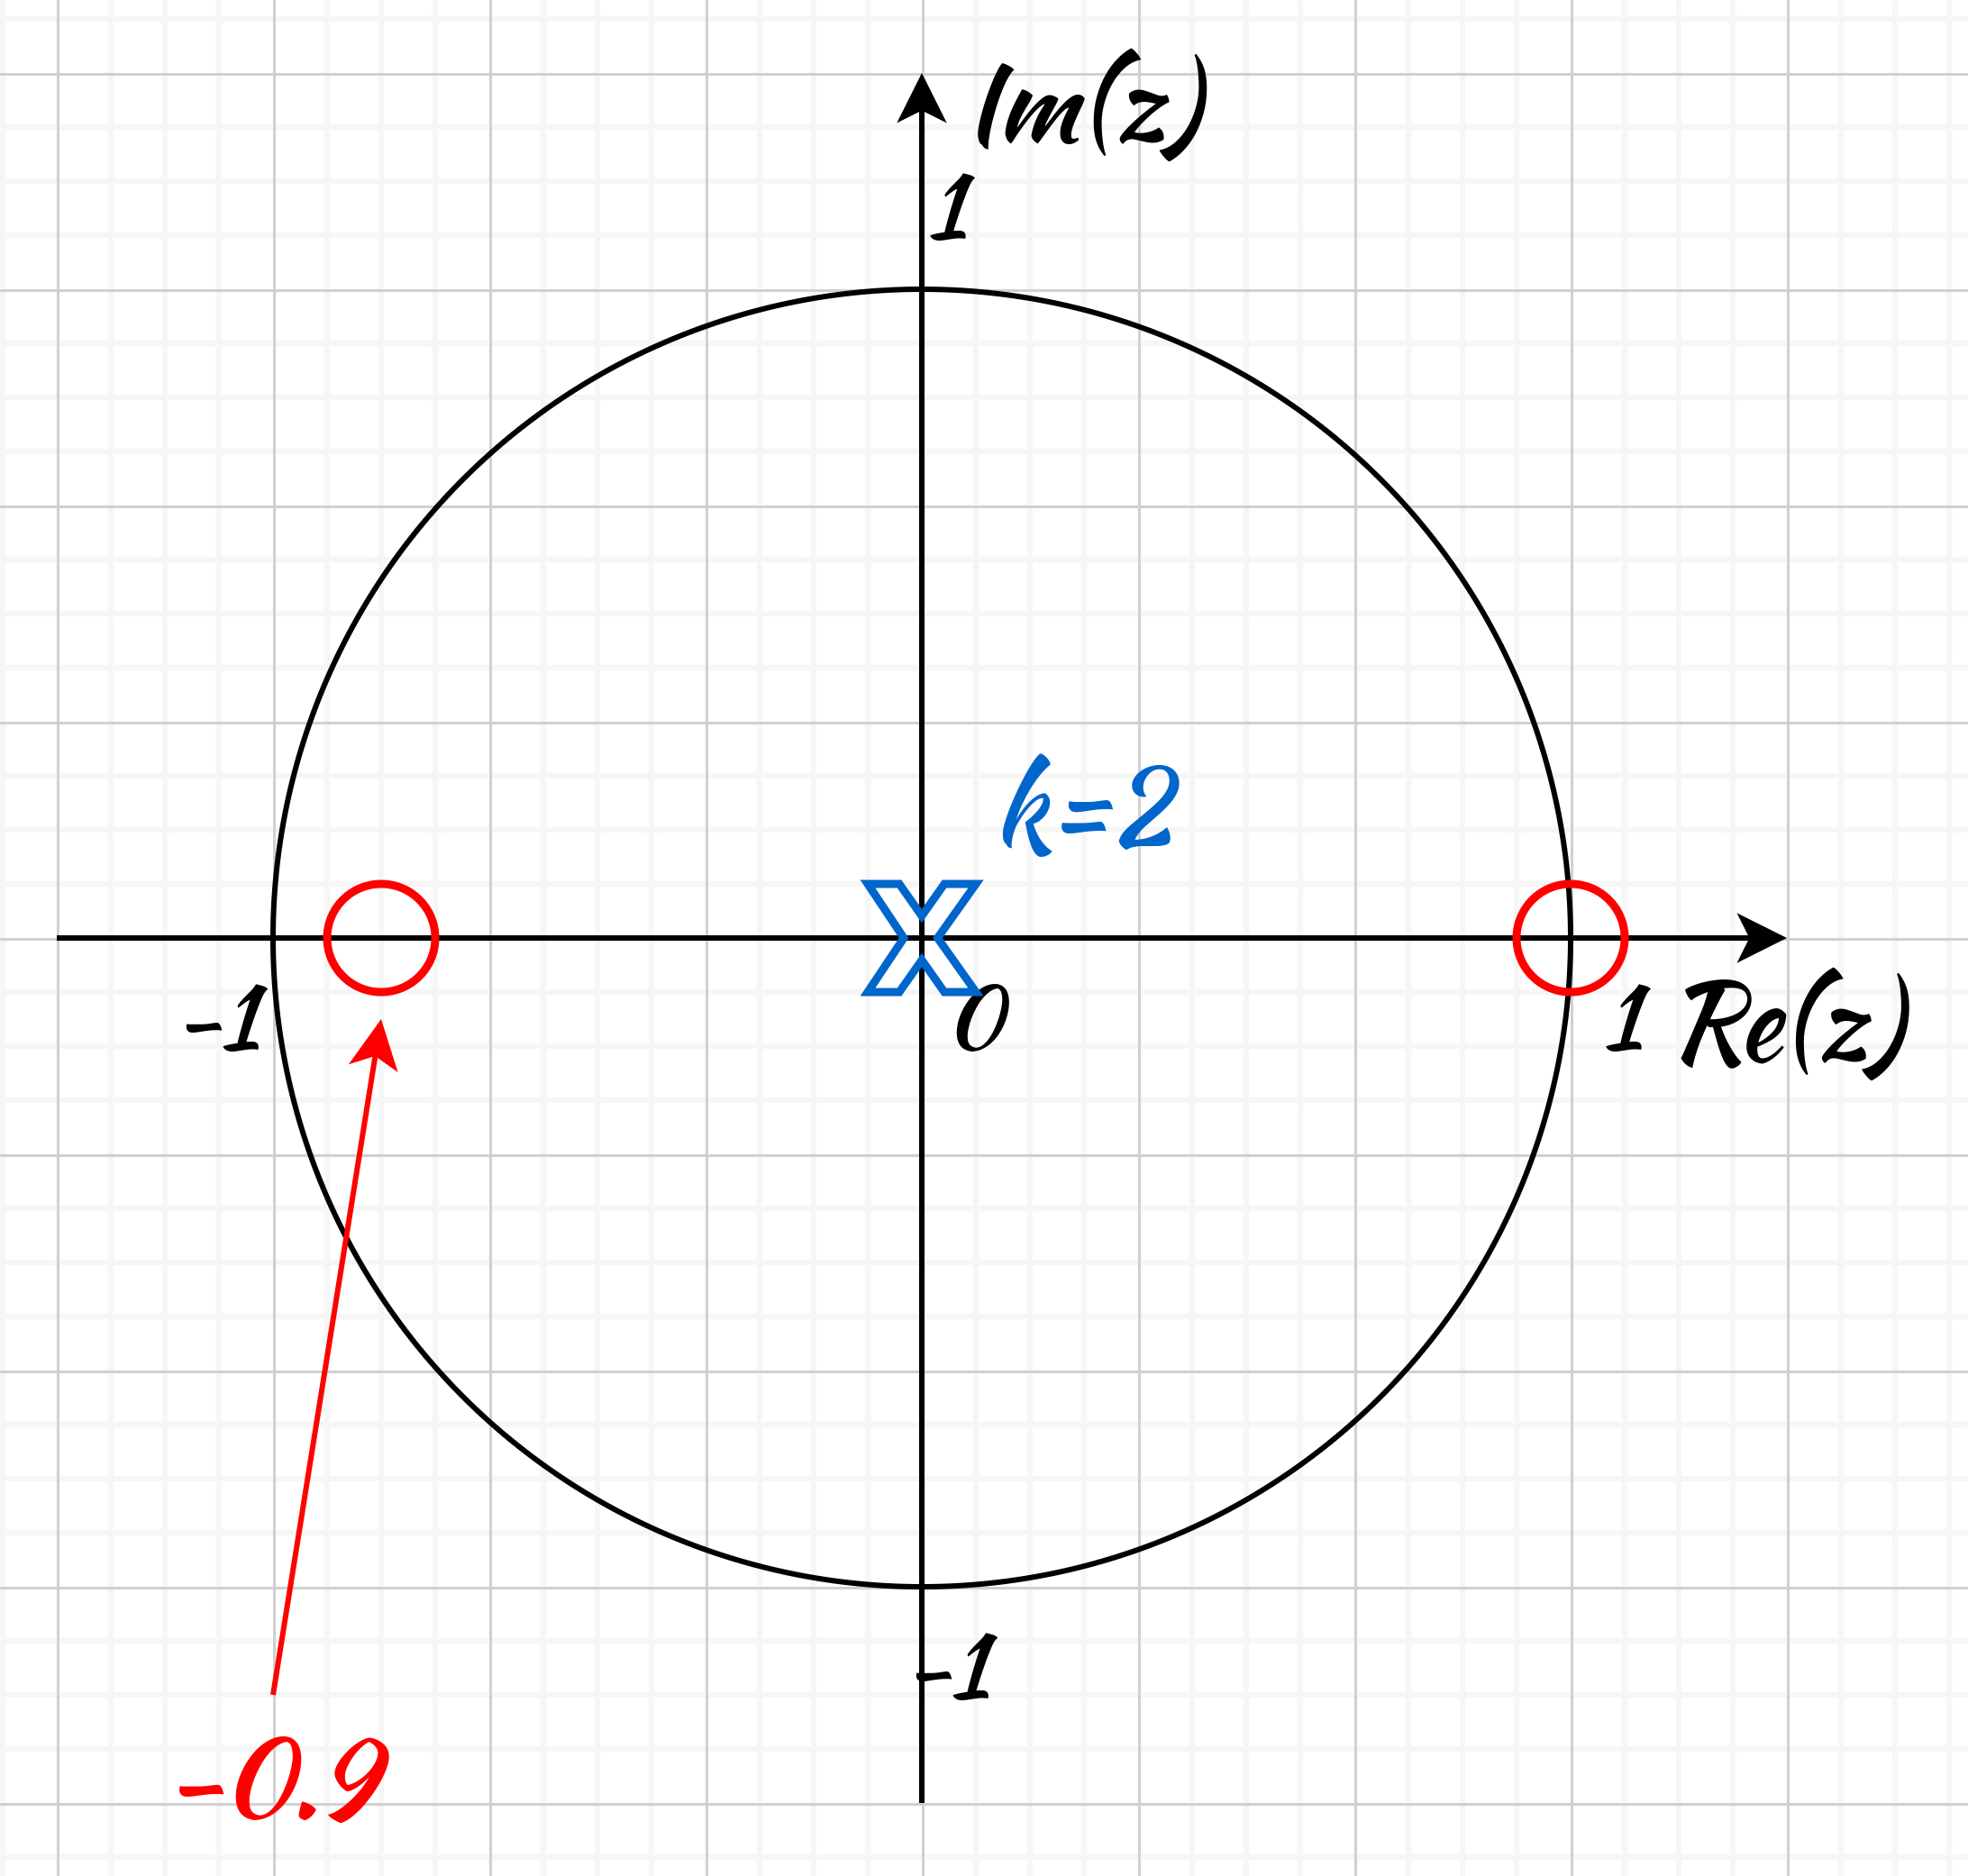
\includegraphics[width=0.4\columnwidth]{pics/fall/12/12-2-1.png}
	\label{fig:12-2-1}
\end{figure}


\begin{equation*}
	\Capit{H}(z) = 1 - 0.1z^{-1} - 0.9z^{-2} =  h[0] + h[1]z^{-1} + h[2]z^{-2},
	\quad \Rightarrow h[k] = 
	\begin{cases}
		1, & \text{если } k = 0,\\
		-0.1, & \text{если } k = 1,\\
		-0.9, & \text{если } k = 2,\\
		0, & \text{иначе}.
	\end{cases}
\end{equation*}

\begin{equation*}
	g[k] = \sum \limits_{m = 0}^{+\infty} h[k + m] = 
	\begin{cases}
		1, & \text{если } k = 0,\\
		0.9, & \text{если } k = 1,\\
		0, & \text{иначе}.
	\end{cases}
\end{equation*}


\begin{figure}[!h]
	\centering
	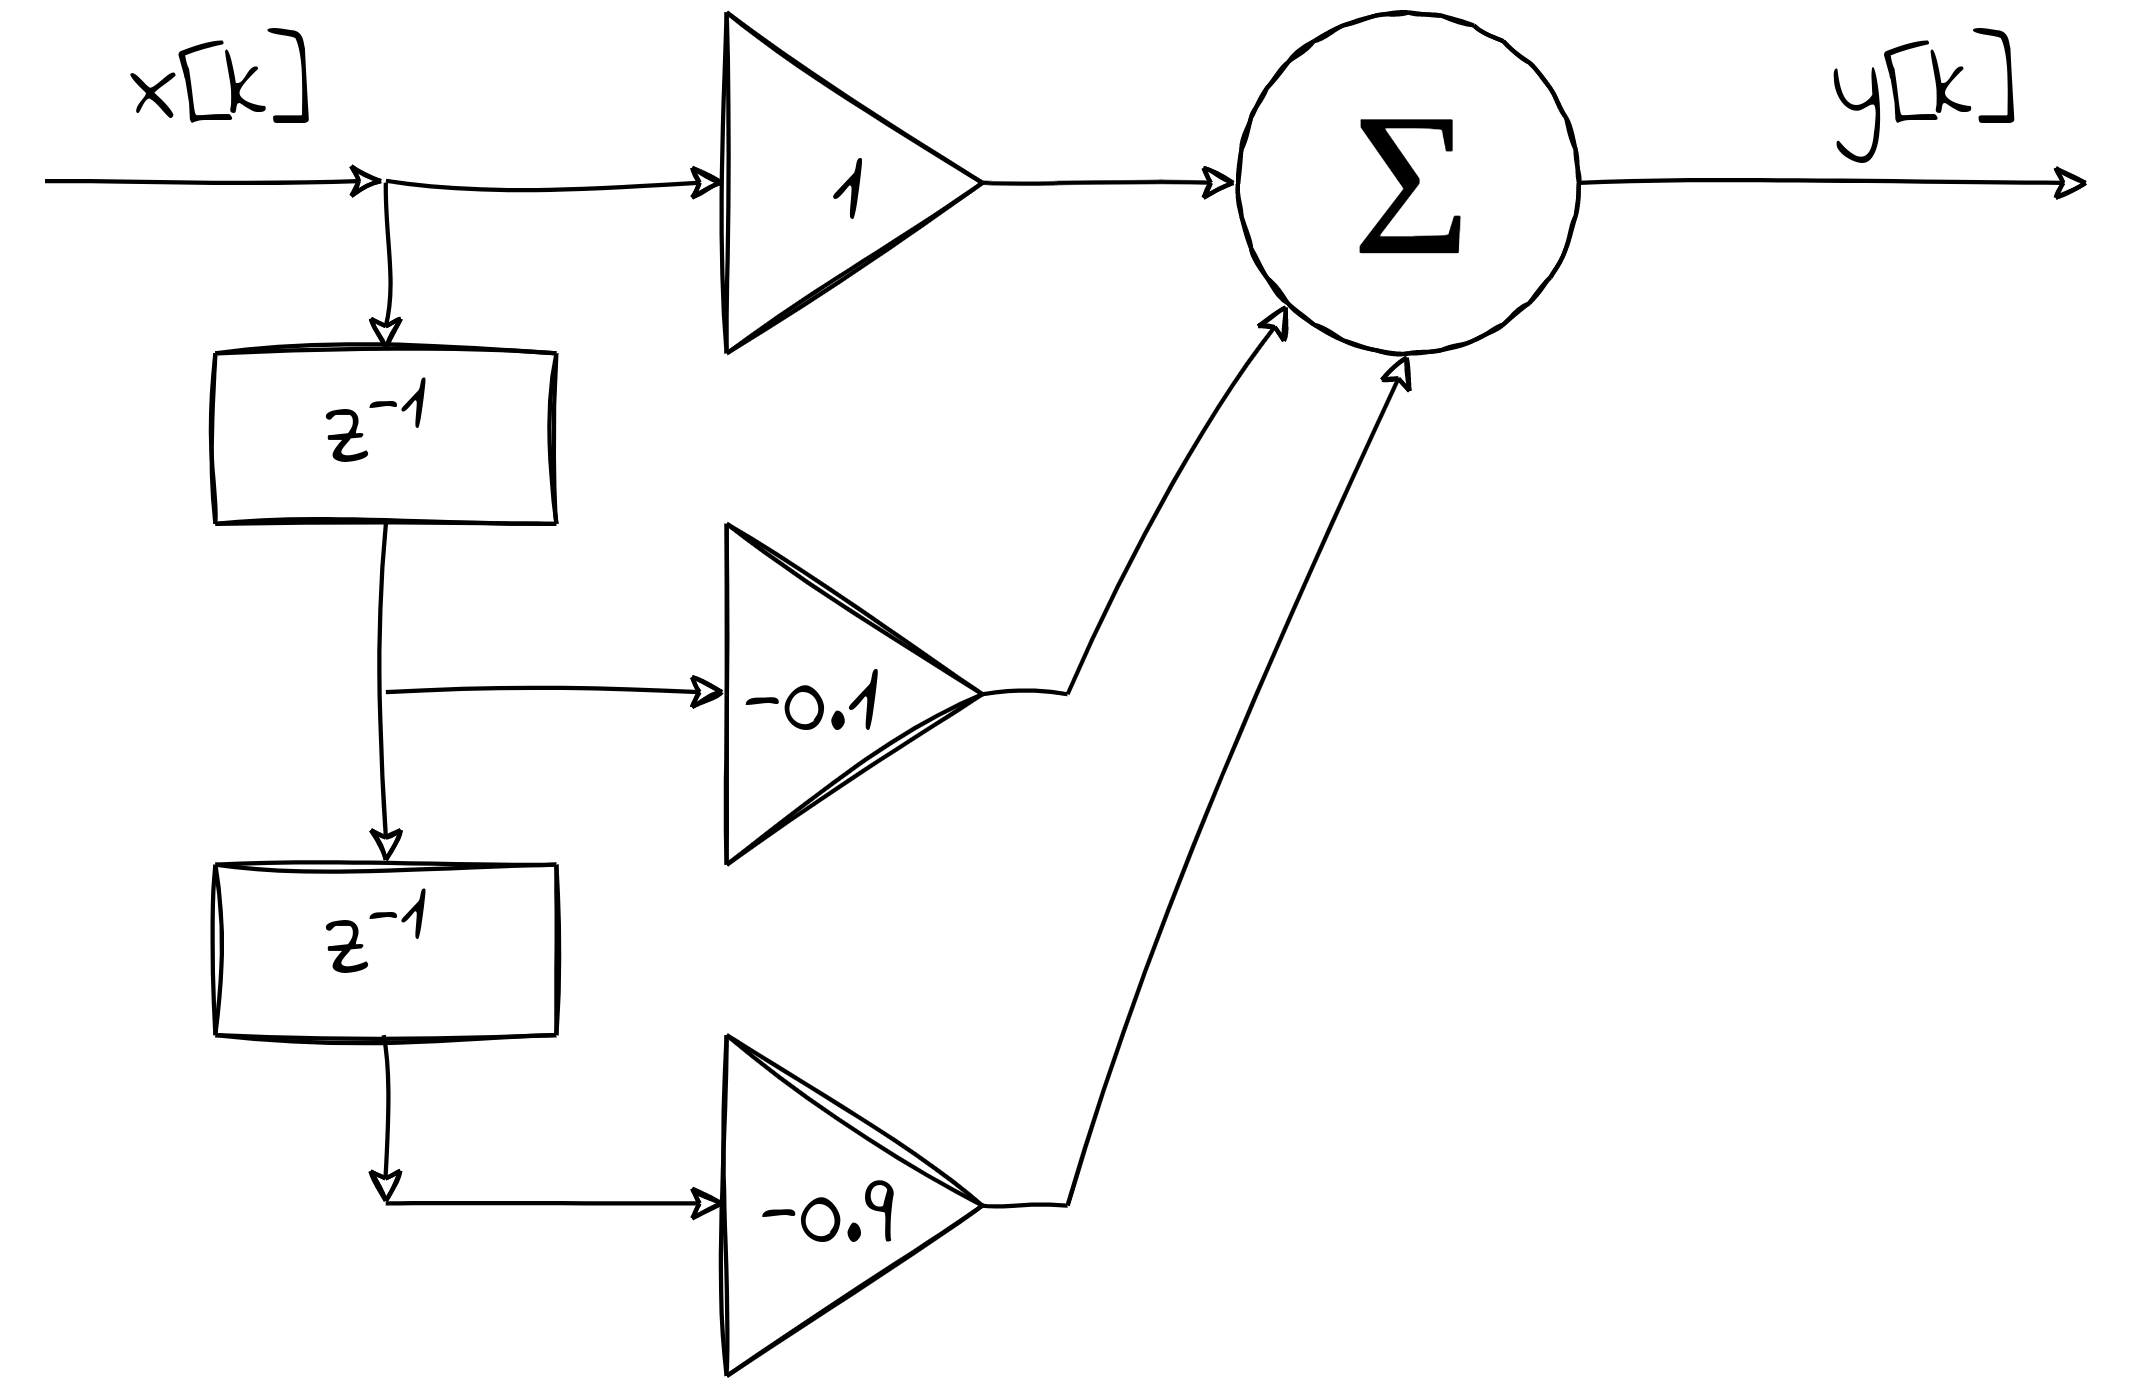
\includegraphics[width=0.75\columnwidth]{pics/fall/12/12-2-2.png}
	\caption{Блок-схема фильтра в прямой форме.}
	\label{fig:12-2-2}
\end{figure}

\begin{figure}[!h]
	\centering
	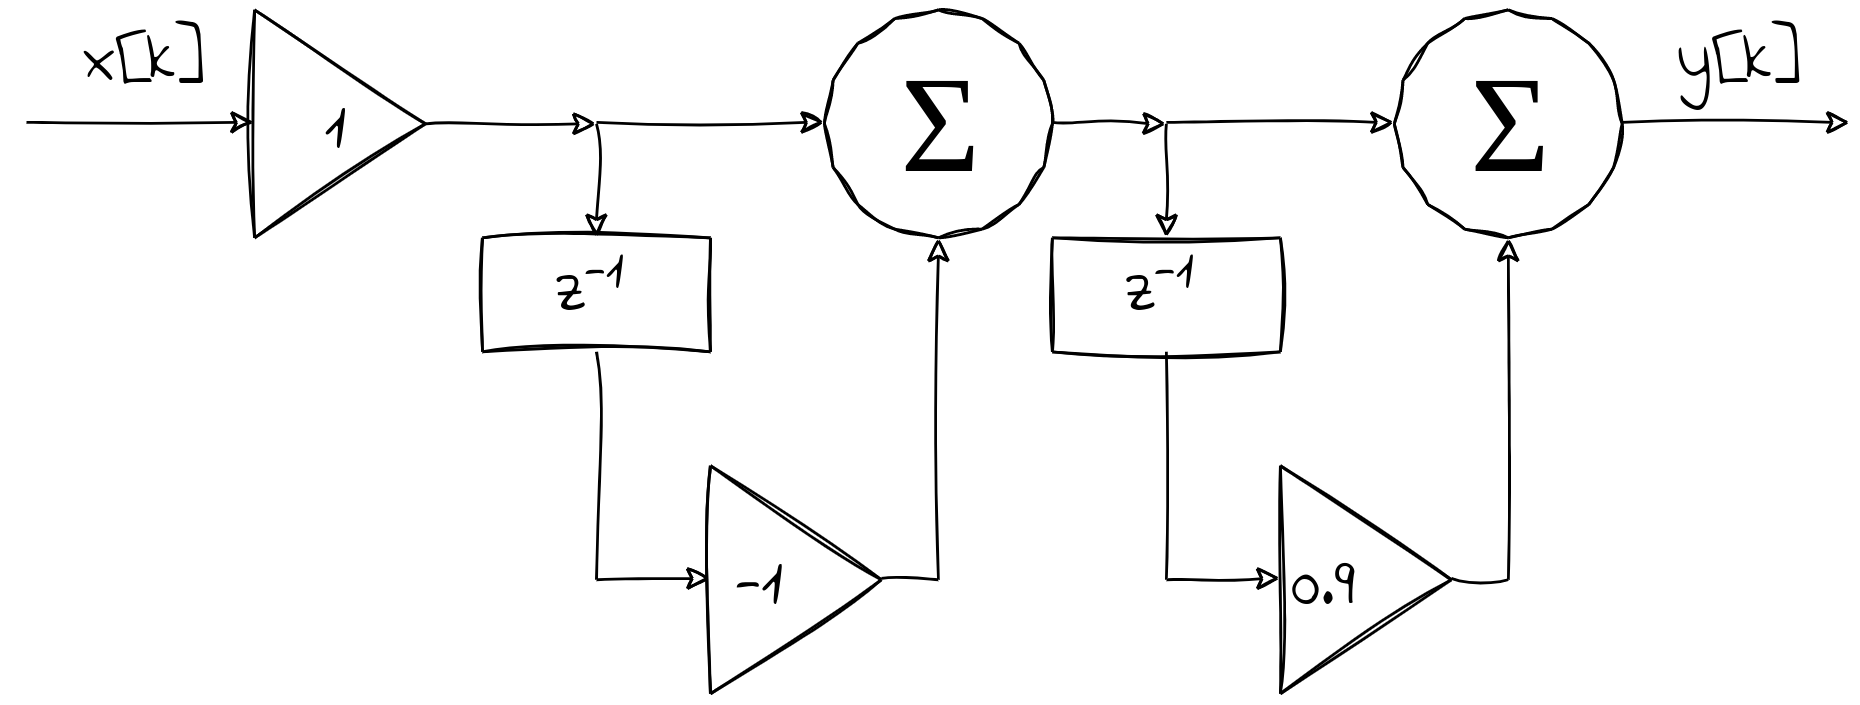
\includegraphics[width=0.75\columnwidth]{pics/fall/12/12-2-3.png}
	\caption{Блок-схема фильтра в виде последовательного соединённых нерекурсивных фильтров первого порядка.}
	\label{fig:12-2-3}
\end{figure}






\section{}
Записать разностное уравнение нерекурсивного фильтра второго порядка, передаточная функция которого содержит два комплексно-сопряженных нуля, расположенных на мнимой оси, а частотная характеристика фильтра $\Capit{H}(\theta)$ равна нулю в точках $\theta = \pm \frac{\pi}{2}$ и единице в точках $\theta = 0$ и $\theta = \pi$. Определить АЧХ и ФЧХ фильтра. Вычислить импульсную характеристику такого фильтра. Определить, будет ли ФЧХ такого фильтра линейной.

Определить, к какому классу частотно-избирательных фильтров его можно отнести:

\begin{enumerate}[label=(\alph*)]
	\item фильтры нижних частот,
	\item фильтры верхних частот,
	\item полосовые фильтры,
	\item режекторные фильтры.
\end{enumerate}

Передаточная функция имеет два комплексно-сопряженных нуля, расположенных на мнимой оси. Без ограничения общности, $z_o = j y$, $y \in \mathbb{R}$. Пусть $\s{k} \in \mathbb{R}$ -- множитель в приведённой форме $\Capit{H}(z)$.

\begin{equation*}
	\Capit{H}(z) = \s{k}(z - z_o)(z - z_o^*) = \s{k} (z - jy)(z + jy) = \s{k}(z^2 + y^2),
	\quad \Rightarrow \Capit{H}(\theta) = \Capit{H}(z)\big|_{z = e^{j \theta}} = \s{k}(e^{2j\theta} + y^2).
\end{equation*}

\begin{align*}
	&\Capit{H}(0) = \Capit{H}(\pi) =  \Capit{H}(\theta)\big|_{\theta = 0} = \s{k}(1 + y^2) = 1.\\
	&\Capit{H}(\pm \pi/2) =  \Capit{H}(\theta)\big|_{\theta = \pm \frac{\pi}{2}} = \s{k}(-1 + y^2) = 0.\\
	&\begin{cases}
		\s{k}(+1 + y^2) = 1\\
		\s{k}(-1 + y^2) = 0\\
	\end{cases} \Leftrightarrow
	\begin{cases}
		y = \pm 1\\
		\s{k} = 0.5\\
	\end{cases}
\end{align*}

\begin{align*}
	&\Capit{H}(\theta) = 0.5(1 + e^{2j\theta}) = 0.5 e^{-j\theta} (e^{j\theta} + e^{-j\theta}) = e^{-j\theta} \cos\theta.\\
	&|\Capit{H}(\theta)| = |\cos\theta|,\quad
	\arg\{\Capit{H}(\theta)\} = \arg\{e^{-j\theta}\} = -\theta, \; \Rightarrow \text{ ФЧХ линейная}.
\end{align*}

Этот фильтр относится к гребенчатым фильтрам, поскольку его АЧХ имеет гребенчатую структуру.
Если же рассматривать главный период, то его можно отнести к режекторным фильтрам.


\setcounter{chapter}{13}
\setcounter{section}{0}
%\chapter*{Неделя 13}
\protect\thispagestyle{fancy}
\section{}
Для нерекурсивного фильтра первого порядка, заданного разностным уравнением
\begin{equation*}
	y[k] = x[k] + ax[k-1]
\end{equation*}

найти значения $a$, при которых

\begin{enumerate}[label=(\alph*)]
	\item для всех частот одинаковая фазовая задержка $\tau_{ph}(\theta) = \text{const}$,
	\item для всех частот одинаковая групповая задержка $\tau_{gr}(\theta) = \text{const}$.
\end{enumerate}

Изобразить ФЧХ для этих случаев на отрезке $\theta \in [-\pi; \pi]$.

\begin{gather*}
	\Capit{H}(z) = 1 + az^{-1}\big|_{z = e^{j \theta}} = 1 + ae^{-j \theta} =
	(1 + a\cos\theta) -ja\sin\theta,\quad \Rightarrow
	\varphi(\theta) = \arg\{\Capit{H}(\theta)\} = -\text{arctg}\left(\frac{a\sin\theta}{1+a\cos\theta}\right).
\end{gather*}

\begin{align*}
	\tau_{ph}(\theta) = -\dfrac{\varphi(\theta)}{\theta}\Delta t = \dfrac{\Delta t}{\theta}\text{arctg}\left(\frac{a\sin\theta}{1+a\cos\theta}\right),\quad
	\tau_{gr}(\theta) = -\dfrac{d\varphi(\theta)}{d\theta}\Delta t = \Delta t \dfrac{d}{d\theta} \left\{ \text{arctg}\left(\frac{a\sin\theta}{1+a\cos\theta}\right) \right\}.
\end{align*}

\begin{gather*}
	\tau_{ph}(\theta) = \text{const} \Leftrightarrow a \in \{0, 1\},\\
	\tau_{gr}(\theta) = \text{const} \Leftrightarrow a \in \{-1, 0, 1\}.
\end{gather*}

\begin{figure}[!h]
	\centering
	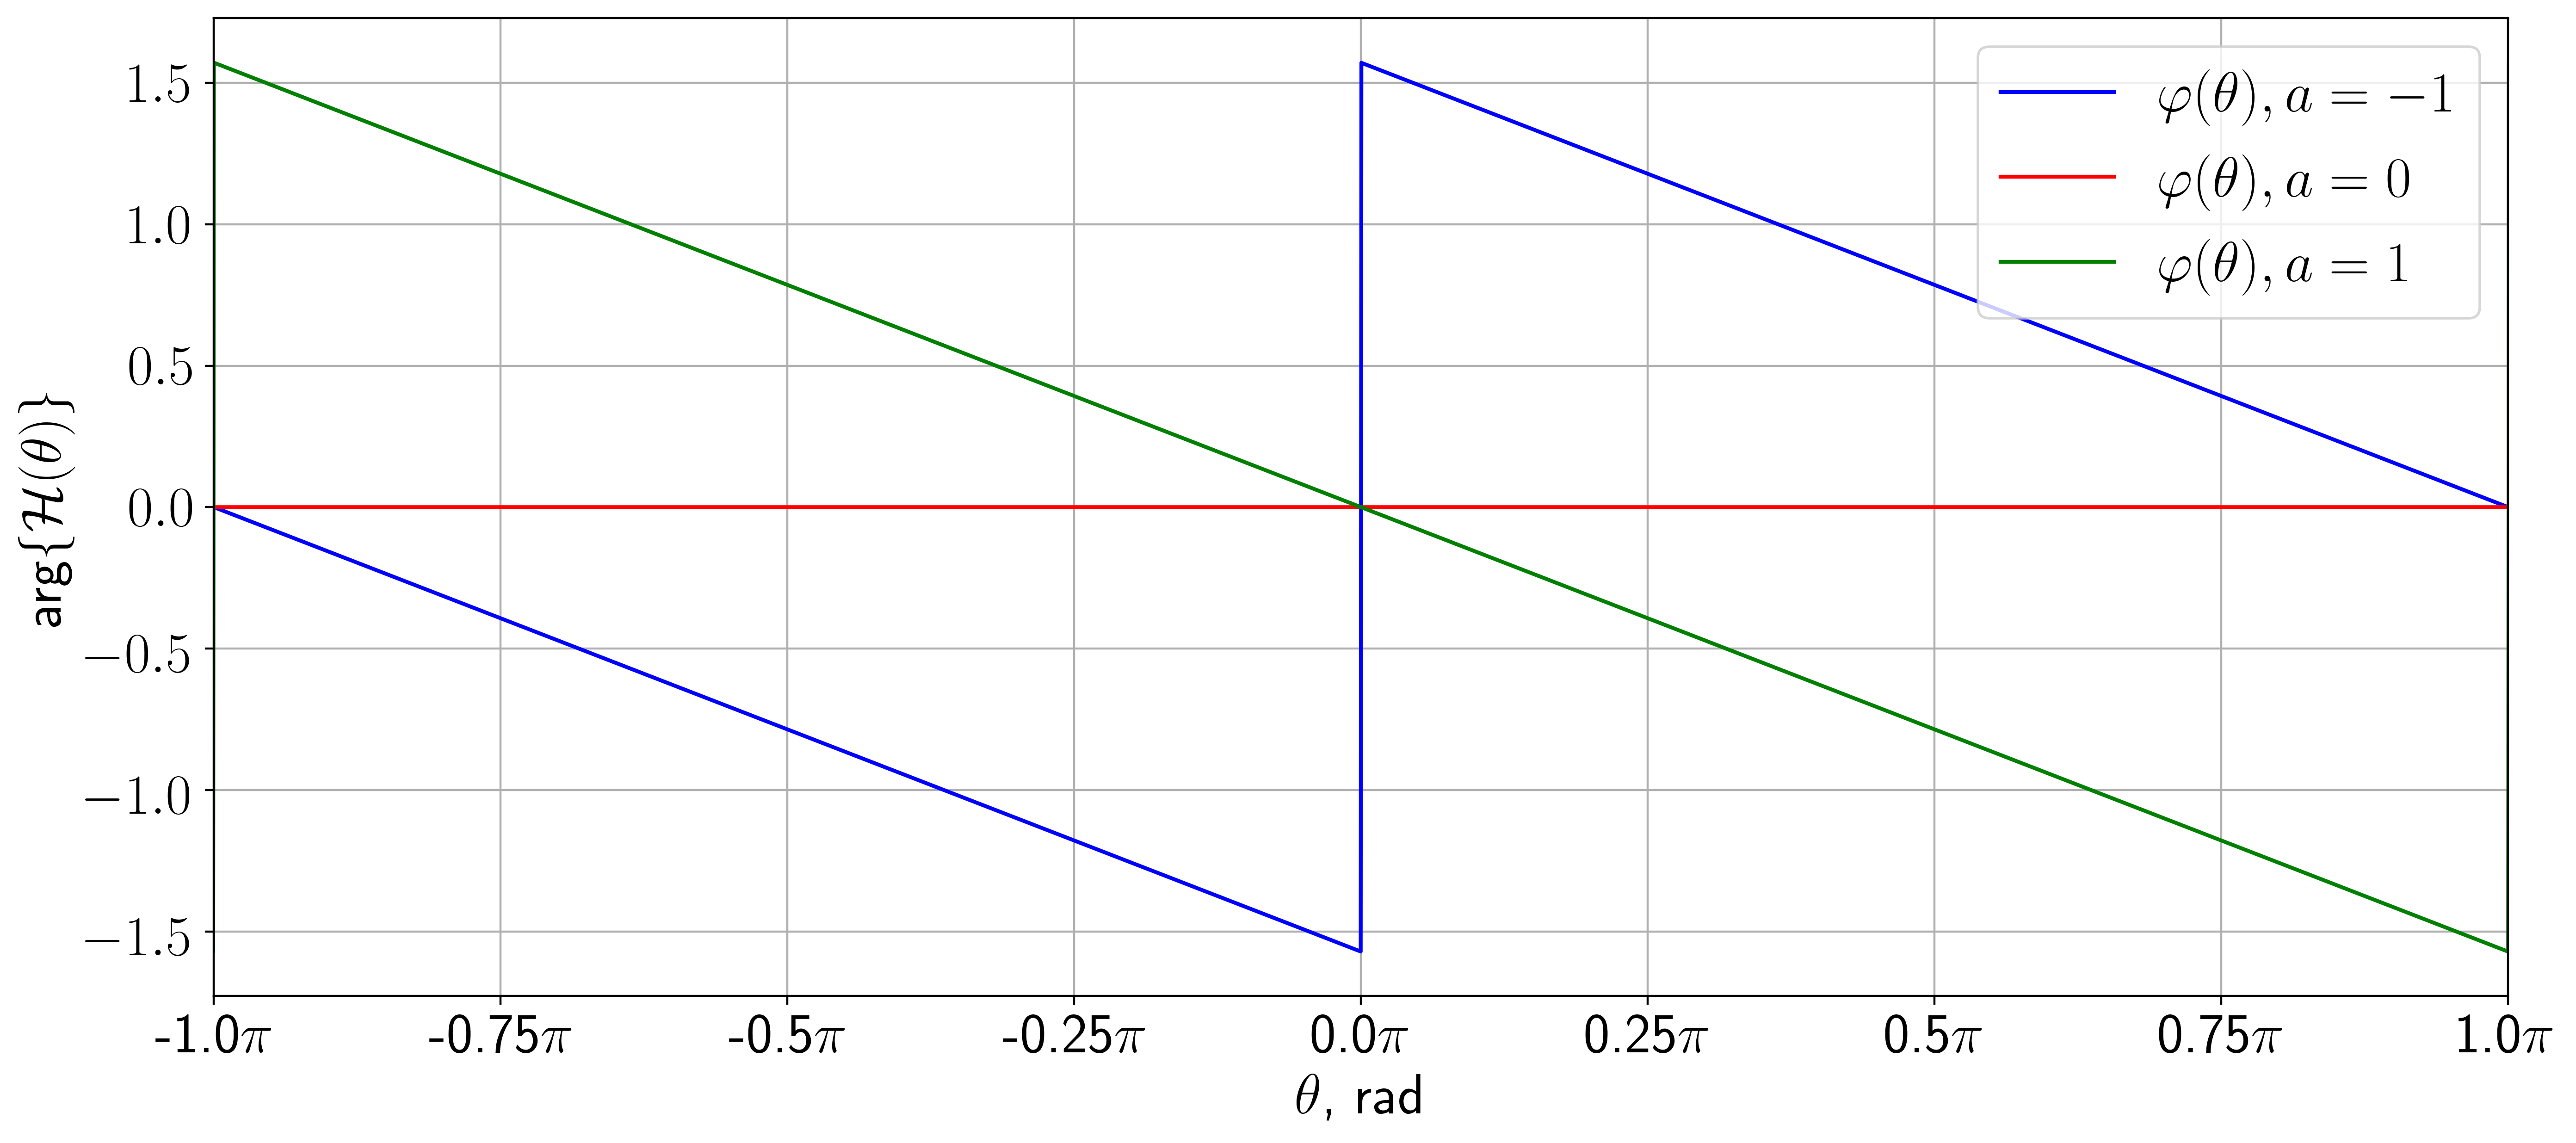
\includegraphics[width=0.8\columnwidth]{pics/fall/13/13-1.png}
	\label{fig:13-1}
\end{figure}


\newpage
\section{}

Определить АЧХ и ФЧХ гребенчатого фильтра $y[k] = x[k] - x[k-N]$.
Является ли ФЧХ линейной?

\begin{equation*}
	\Capit{H}(z) = 1 - z^{-N}\big|_{z = e^{j \theta}} = 1 - \exp\big(-jN \theta \big) =
	2 j\exp\Big(-j \frac{N \theta}{2}\Big) \sin\Big(\frac{N \theta}{2}\Big) =
	2 \exp\Big(j \Big(\frac{\pi}{2} - \frac{N \theta}{2}\Big)\Big) \sin\Big(\frac{N \theta}{2}\Big).
\end{equation*}

\begin{gather*}
	|\Capit{H}(\theta)| = 2\Big|\sin\Big(\frac{N \theta}{2}\Big)\Big|,\\
	\varphi(\theta) = \frac{\pi}{2} - \frac{N \theta}{2},\;\text{где } 0 \leq \theta \leq \frac{2\pi}{N} \text{ с периодом } T_{\theta} = \dfrac{2\pi}{N}.\quad \text{(С учётом смены знака синусом.)}
\end{gather*}

ФЧХ данного фильтра является линейной (кусочно-линейной).

\begin{figure}[!h]
	\centering
	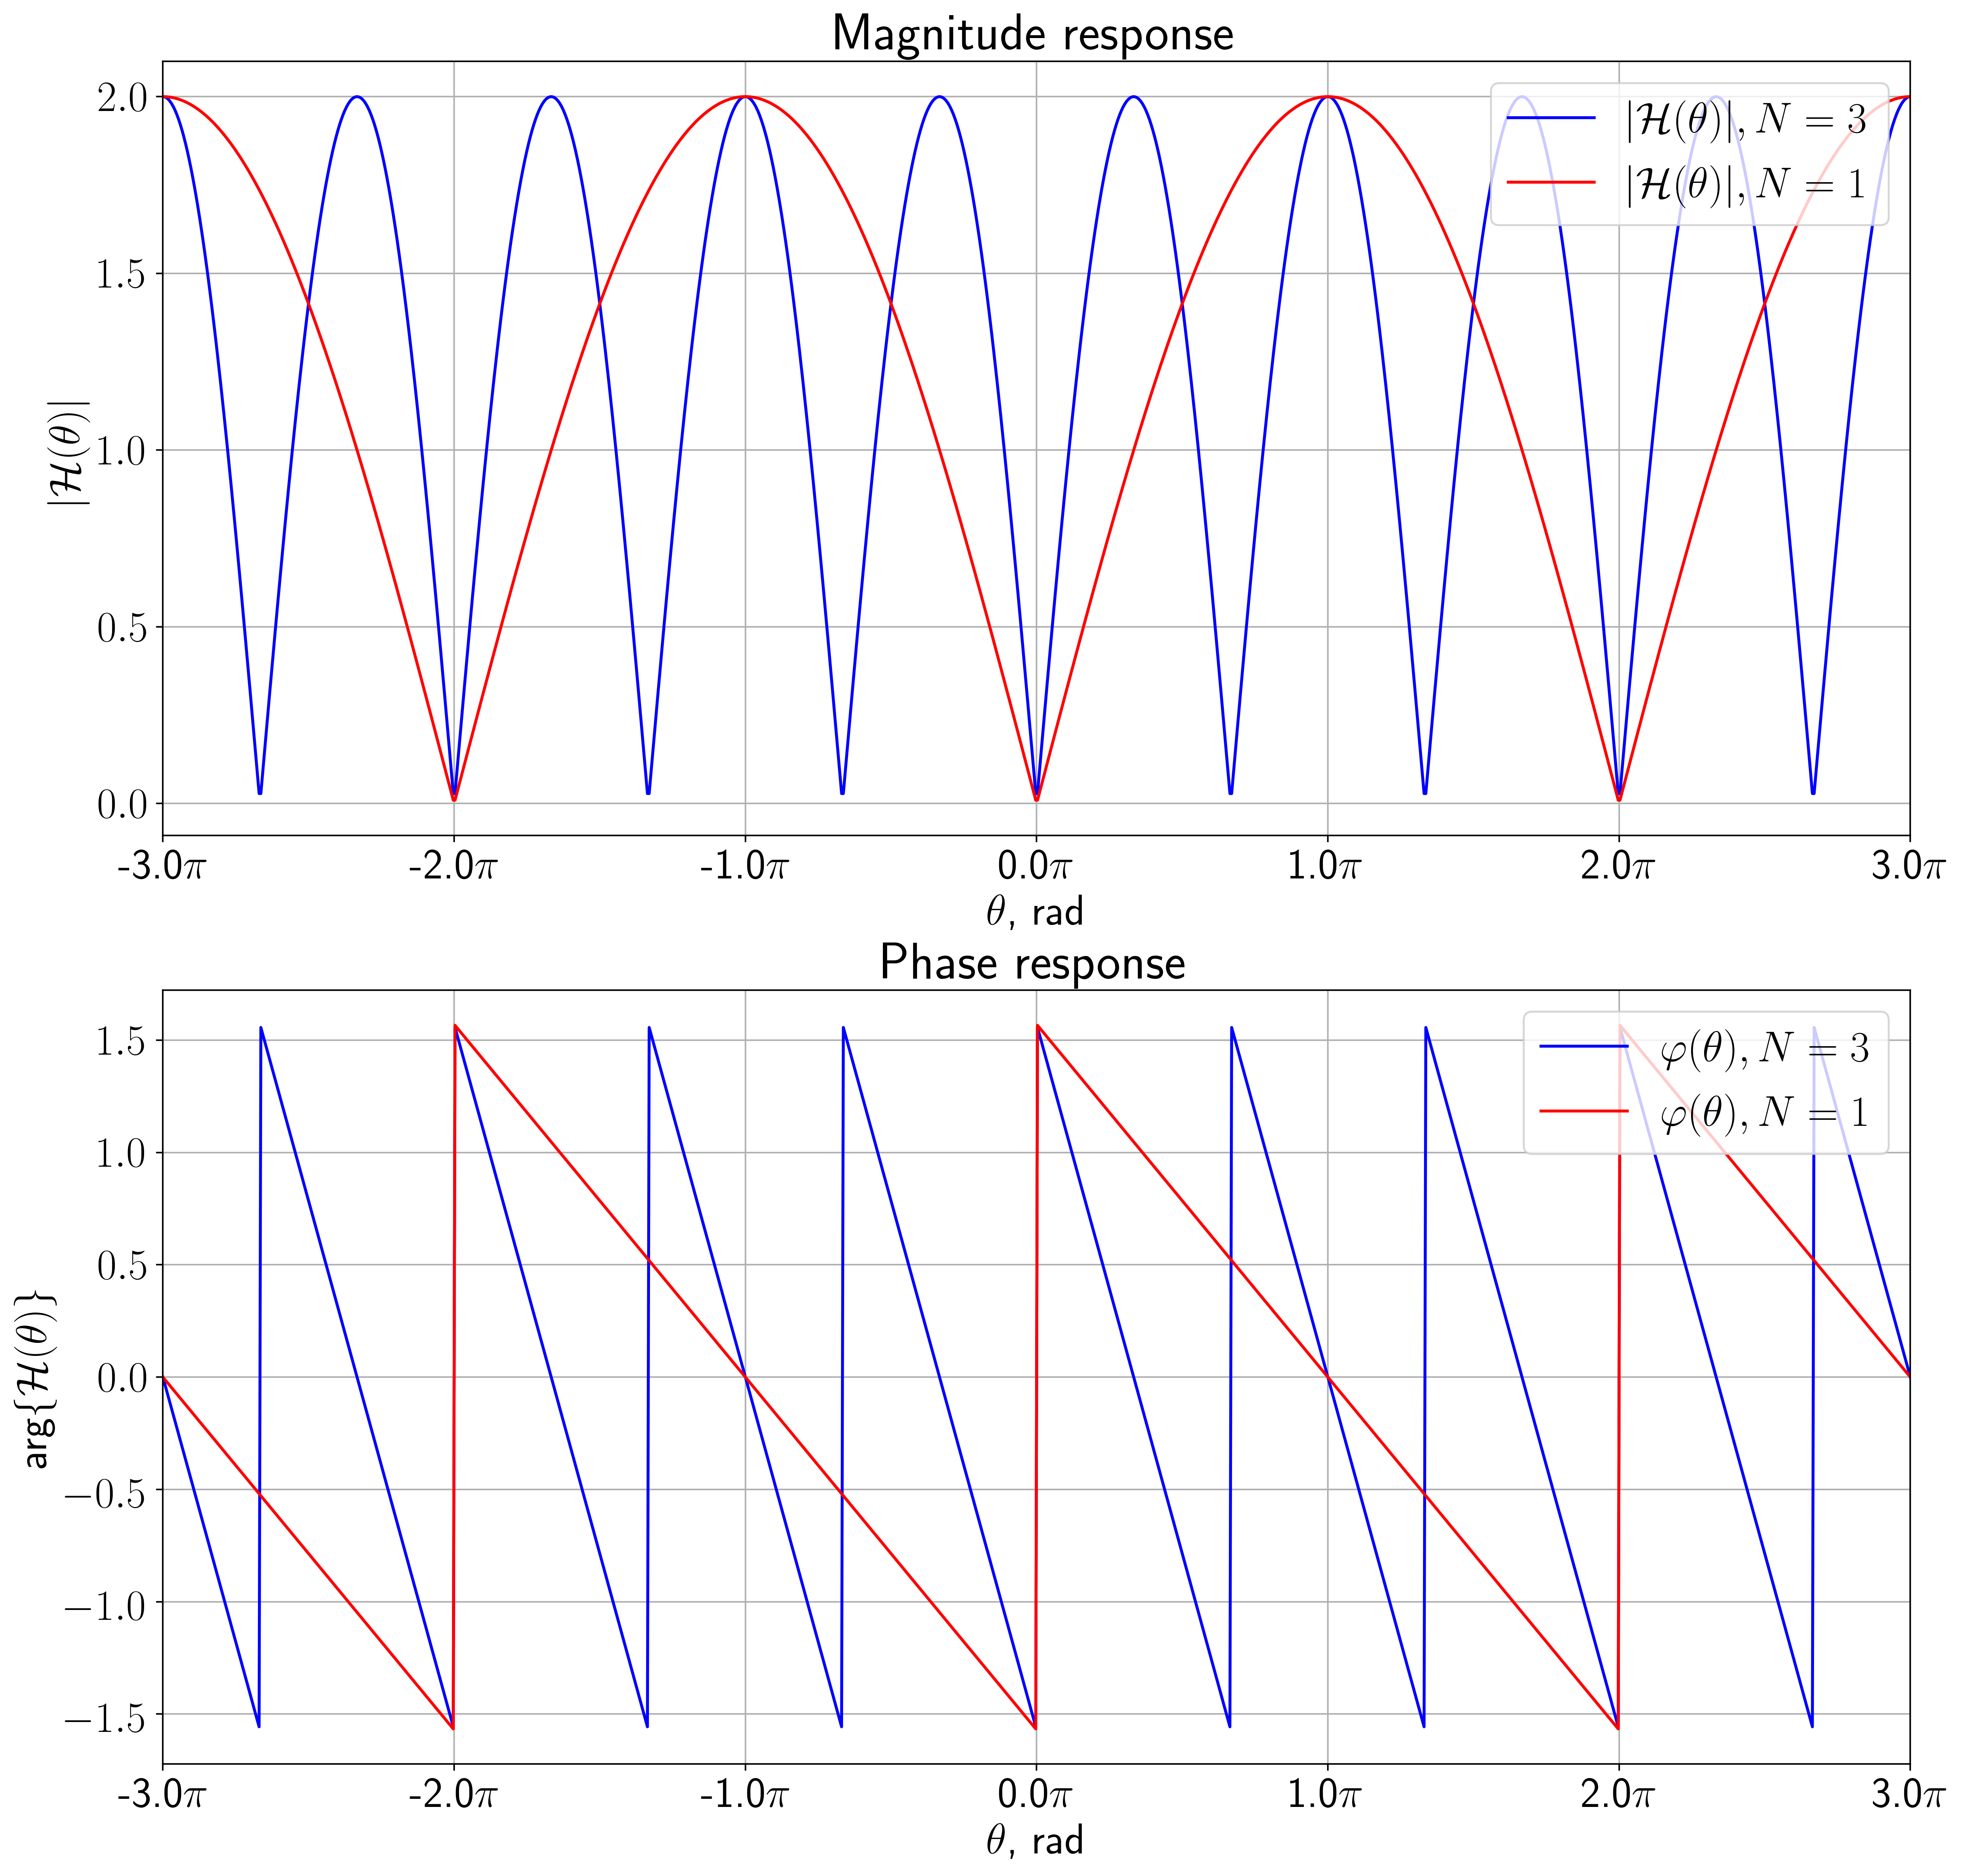
\includegraphics[width=0.8\columnwidth]{pics/fall/13/13-2.png}
	\label{fig:13-2}
\end{figure}


\newpage
\section{}

Определить ФЧХ CIC-фильтра с передаточной функцией
\begin{equation*}
	\Capit{H}_2(z) = \left(\dfrac{1 - z^{-N}}{1 - z^{-1}}\right)^2.
\end{equation*}

Будет ли ФЧХ такого фильтра линейной на $\theta \in [-\pi; \pi]$?
Как это соотносится с видом импульсной характеристики такого фильтра?

\begin{equation*}
	\Capit{H}_2(z) = \left(\dfrac{1 - z^{-N}}{1 - z^{-1}}\right)^2\Big|_{z = e^{j \theta}} =
	\left(\dfrac{1 - e^{-jN\theta}}{1 - e^{-j\theta}}\right)^2 =
	\dfrac{e^{-jN\theta}}{e^{-j\theta}} \dfrac{\sin^2\left(\frac{N \theta}{2}\right)}{\sin^2\left(\frac{\theta}{2}\right)} =
	e^{-j(N-1)\theta} \cdot \dfrac{\sin^2\left(\frac{N \theta}{2}\right)}{\sin^2\left(\frac{\theta}{2}\right)}.
\end{equation*}

\begin{equation*}
	\varphi(\theta) = -j(N-1)\theta + \frac{2\pi}{(N-1)}m,\; m \in \mathbb{Z}.
\end{equation*}

ФЧХ данного фильтра является линейной (кусочно-линейной). Это означает, что импульсная характеристика должна иметь симметричный или антисимметричный вид.
Действительно, импульсная характеристика данного фильтра содержит $2N-1$ ненулевых отсчётов и является дискретной свёрткой двух последовательностей единичных импульсов длины $N$. Такая свёртка имеет симметричный треугольный вид.

\begin{figure}[!h]
	\centering
	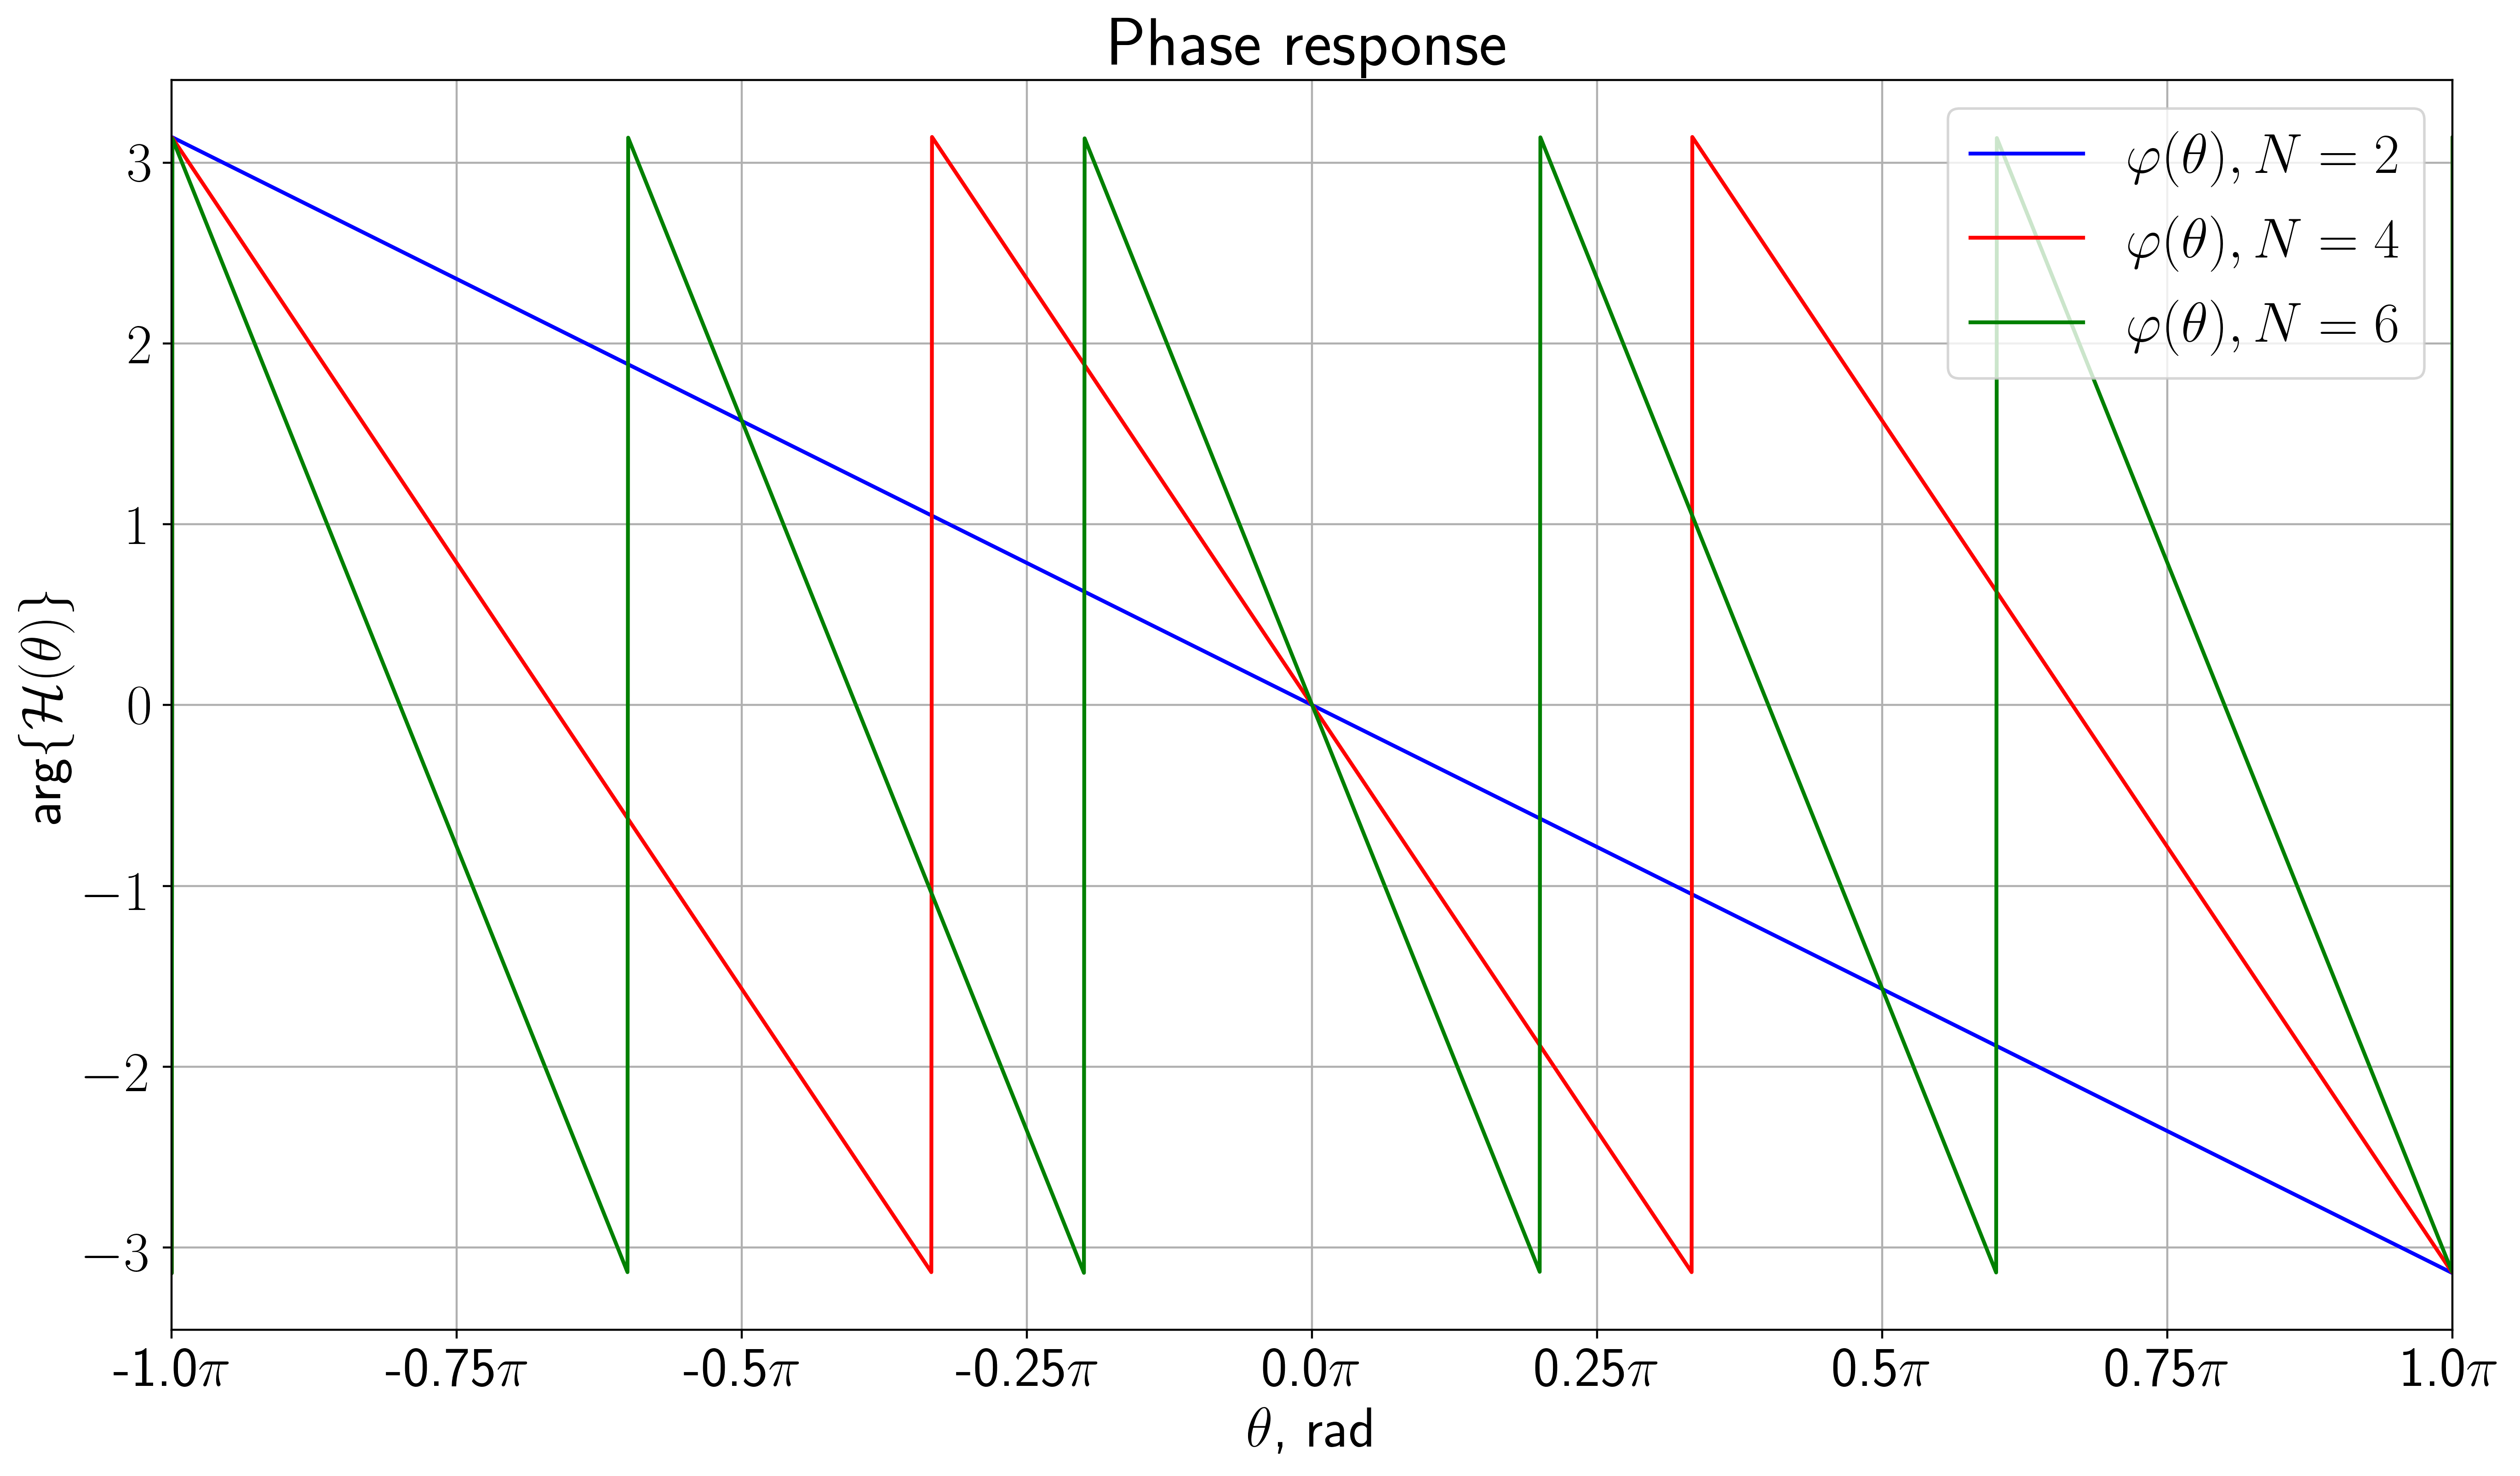
\includegraphics[width=0.8\columnwidth]{pics/fall/13/13-3.png}
	\label{fig:13-3}
\end{figure}



\part{Spring term}

\setcounter{chapter}{1}
\setcounter{section}{0}
%\chapter*{Неделя 1}
\protect\thispagestyle{fancy}
\setcounter{section}{0}

\section{}
Вычислить ДПФ и ДВПФ для окна Хэмминга (окна для ДПФ) длины $N=16$
\begin{equation*}
\s{w}[k] = \begin{cases}
0.54 - 0.46\cos\left(\frac{2\pi k}{N}\right),& \text{ при } 0 \leq k \leq N-1, \\
0,& \text{ при других }k.
\end{cases}
\end{equation*}
Построить графики действительной и мнимой части коэффициентов ДПФ на одном периоде.
\begin{equation*}
\s{w}[k] = 0.54 - 0.46\cos\left(\frac{2\pi k}{N}\right) =
0.54 - 0.23 \cdot \left[\exp\left(+j\frac{2\pi k}{N}\right) + \exp\left(-j\frac{2\pi k}{N}\right)\right],
\quad k \in [0, N-1].
\end{equation*}

По теореме смещения для ДВПФ, получим, что
\begin{equation*}
\Capit{W}(\nu) = \sum \limits_{k = 0}^{N-1} \s{w}[k]e^{-j2\pi \nu k} =
0.54\Capit{W}_{\Capit{D}}(\nu) - 0.23 \cdot \left[ \Capit{W}_{\Capit{D}}\left(\nu - \frac{1}{N}\right)  + \Capit{W}_{\Capit{D}}\left(\nu + \frac{1}{N}\right)\right]^{\footnotemark}.
\end{equation*}

\footnotetext{$\Capit{W}_{\Capit{D}}(\nu) = \dfrac{\sin (N \pi \nu)}{\sin(\pi \nu)}e^{-j(N-1)\pi \nu}$ -- ДВПФ прямоугольного окна (окна Дирихле) из $N$ отсчётов.}

Аналогичным образом получаем ДПФ окна Хэмминга:
\begin{equation*}
\Capit{W}[n] = \begin{cases}
+0.54N,& \text{ если } n = mN,\; m \in \mathbb{Z}, \\
-0.23N,& \text{ если } n = mN\pm1,\; m \in \mathbb{Z}, \\
0,& \text{ иначе}.
\end{cases}
\end{equation*}

\begin{figure}[!h]
	\centering
	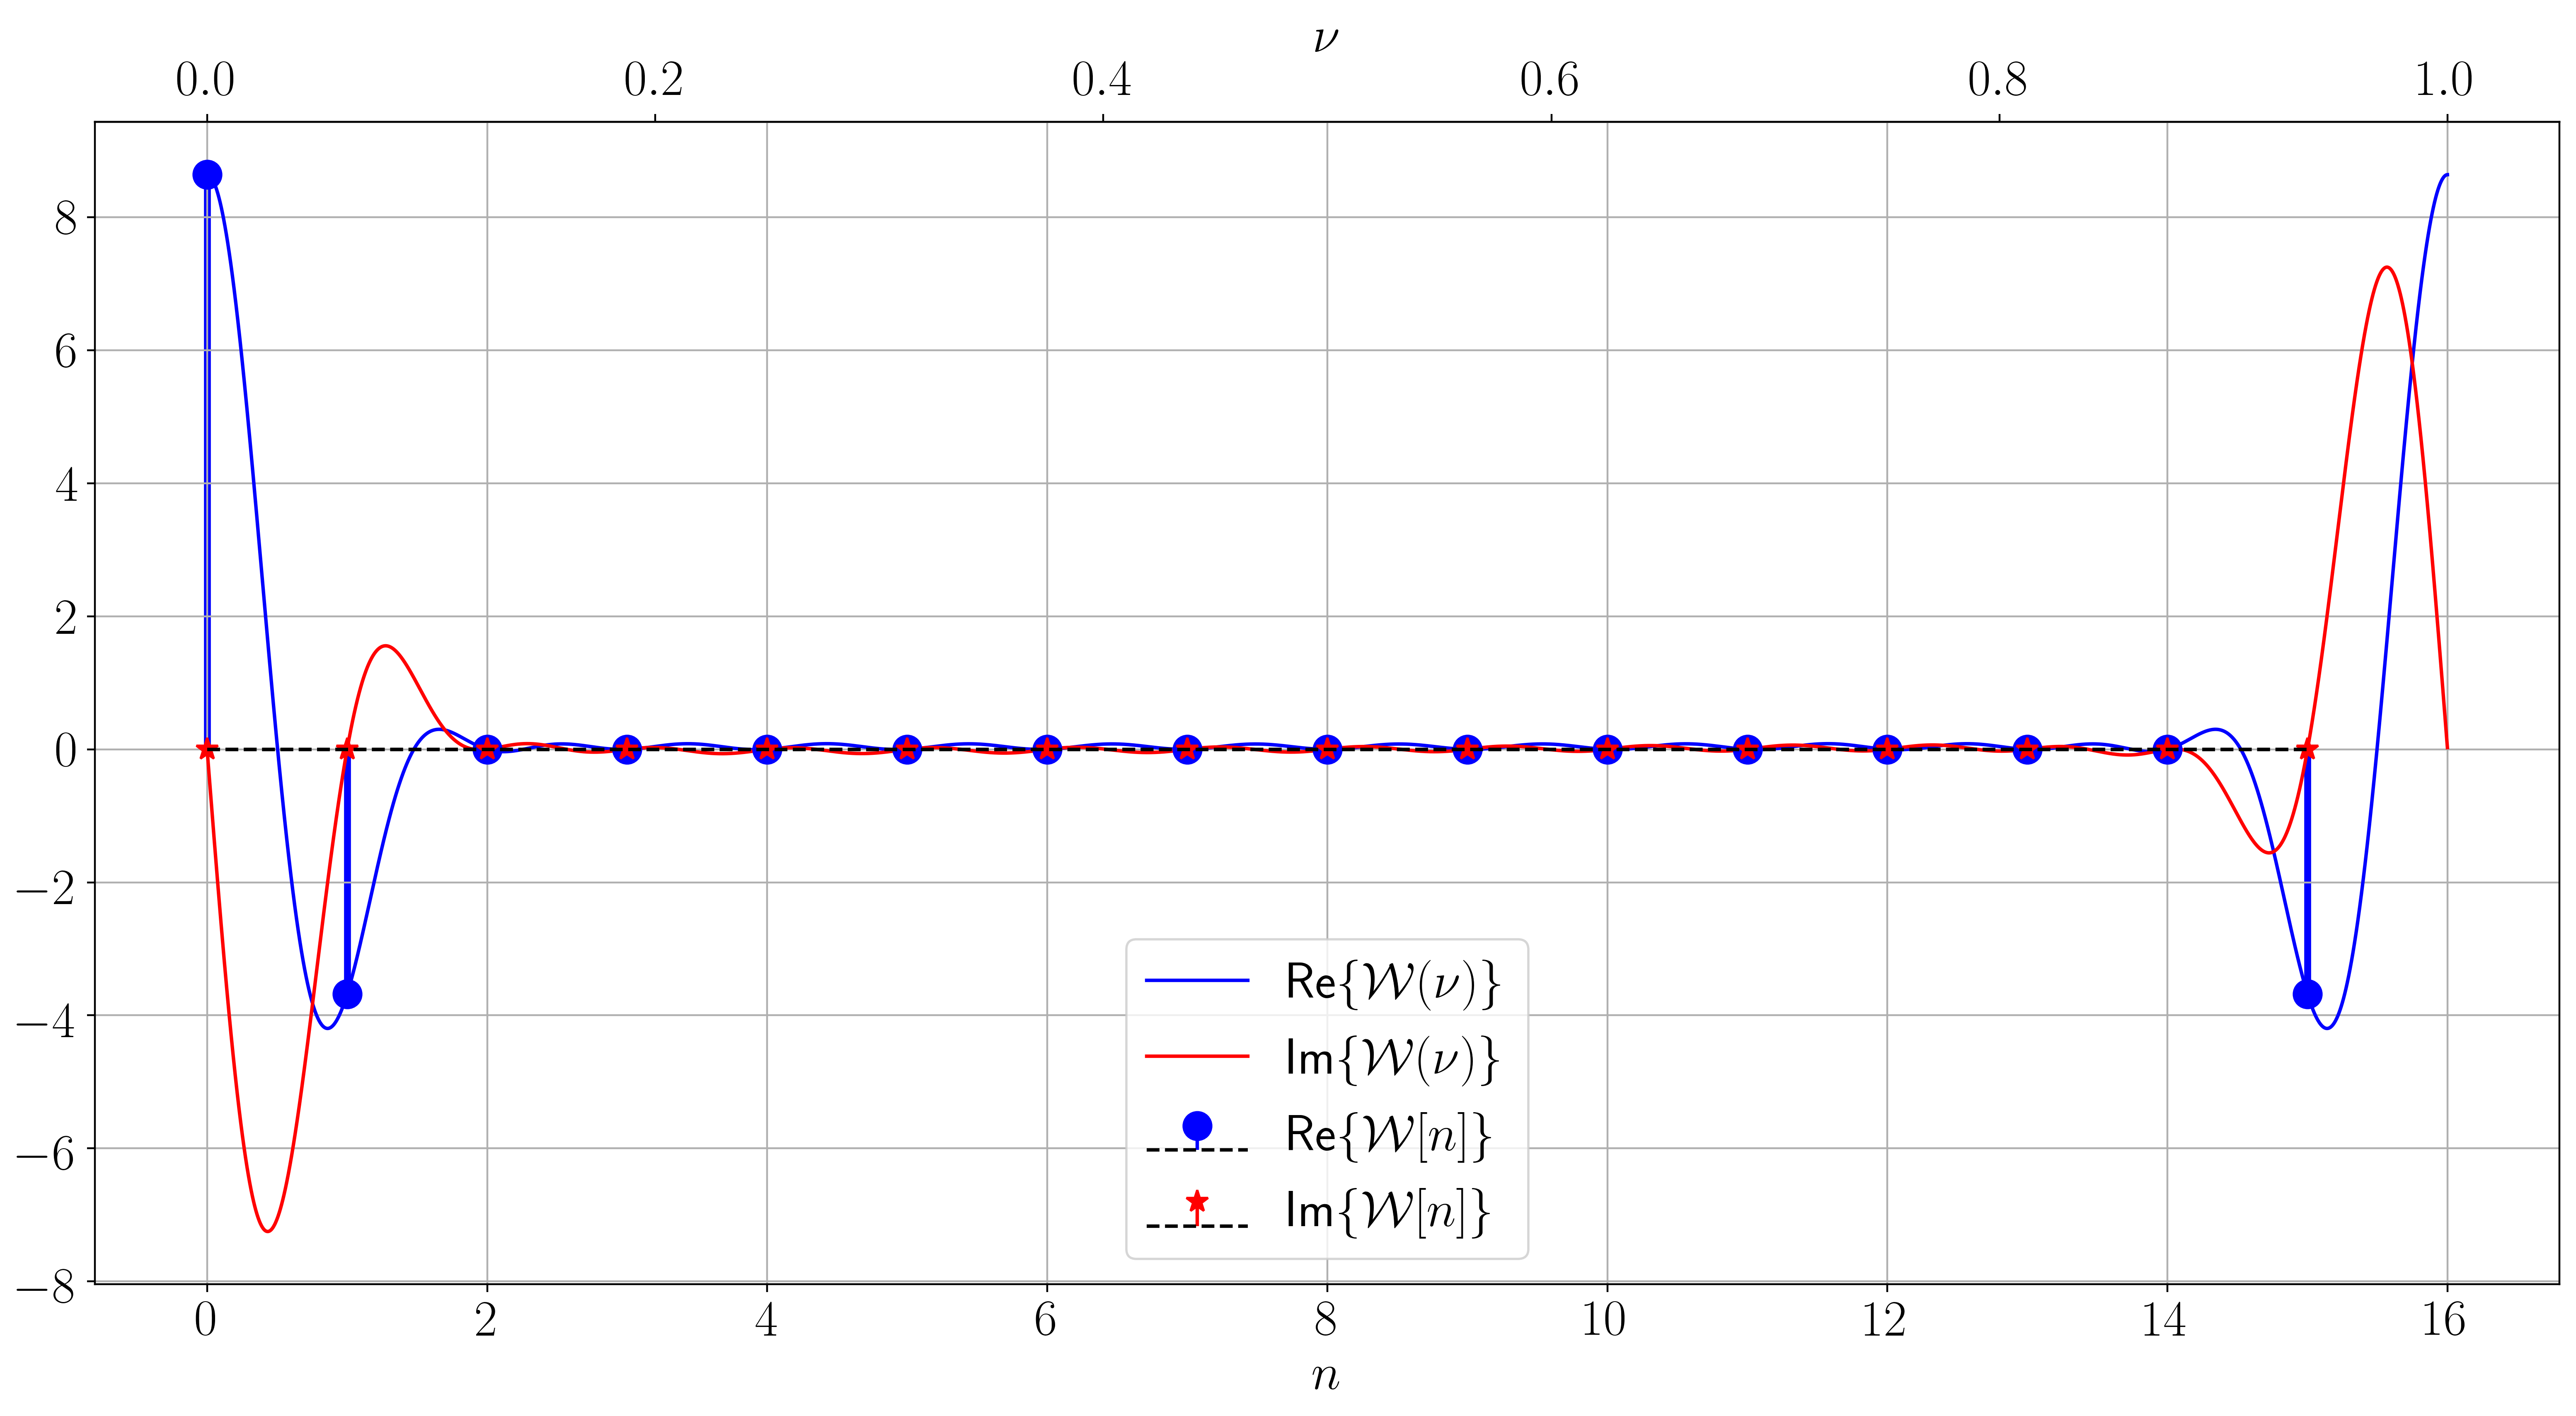
\includegraphics[width=1.0\columnwidth]{pics/spring/1/1-1.png}
	%\caption{.}
	\label{fig:1-1}
\end{figure}

\newpage
\section{}
Предположим, что требуется провести ДПФ-анализ сигнала $x[k]$ с использованием окна Ханна
$\s{w}[k]$. Размерность ДПФ, длина окна и длина сигнала равны $N$. Доказать, что для вычисления ДПФ $\Capit{Y}[n]$ сигнала $x[k]\s{w}[k]$ достаточно провести $2N$ сдвигов на один двоичный разряд и $2N$ сложений для коэффициентов ДПФ $\Capit{X}[n]$ последовательности $x[k]$, т.е. показать, что

\begin{equation*}
\Capit{Y}[n] = \dfrac{1}{2}\left(\Capit{X}[n] - \dfrac{1}{2}\left(\Capit{X}[n-1]_N + \Capit{X}[n+1]_N \right)\right).
\end{equation*}

\begin{align*}
y[k] &= x[k]\s{w}[k] = x[k]\left(\dfrac{1}{2} - \dfrac{1}{2}\cos\left(\dfrac{2\pi k}{N}\right)\right) = 
\dfrac{1}{2}x[k]\left(1 - \dfrac{1}{2}\left[\exp\left(+j\frac{2\pi k}{N}\right) + \exp\left(-j\frac{2\pi k}{N}\right)\right]\right) = \\
&= \dfrac{1}{2}\left(x[k] - \dfrac{1}{2}\left[x[k]\exp\left(+j\frac{2\pi k}{N}\right) + x[k]\exp\left(-j\frac{2\pi k}{N}\right)\right]\right).
\end{align*}

Тогда с применением теоремы смещения для ДПФ получим:
\begin{align*}
\Capit{Y}[n] &= \sum \limits_{k=0}^{N-1}y[k]\exp\left(-j \dfrac{2\pi}{N} nk \right) = 
\sum \limits_{k=0}^{N-1}x[k]\left(\dfrac{1}{2} - \dfrac{1}{2}\cos\left(\dfrac{2\pi k}{N}\right)\right)\exp\left(-j \dfrac{2\pi}{N} nk \right) = \\
&= \dfrac{1}{2}\left(\sum \limits_{k=0}^{N-1}x[k]\exp\left(-j \dfrac{2\pi}{N} nk \right) - \dfrac{1}{2}\left[\sum \limits_{k=0}^{N-1} x[k]\exp\left(-j \dfrac{2\pi}{N} (n-1)k \right)
+ \sum \limits_{k=0}^{N-1} x[k]\exp\left(-j \dfrac{2\pi}{N} (n+1)k \right)\right]\right) = \\
&=\dfrac{1}{2}\left(\Capit{X}[n] - \dfrac{1}{2}\Bigg[\Capit{X}[n-1]_N + \Capit{X}[n+1]_N \Bigg]\right).
\end{align*}

\newpage
\section{}
Вычислить ДВПФ и ДПФ последовательности $y[k] = x[k]\s{w}[k]$, где $x[k] = \sin\Big(2\pi\dfrac{3}{16}k\Big)$, a $\s{w}[k]$ --- окно Ханна для ДПФ длины $N = 16$.
Построить графики действительной и мнимой части коэффициентов ДПФ на одном периоде.

\begin{align*}
y[k] &= x[k]\s{w}[k] =  \sin\left(2\pi\dfrac{3}{16}k\right)\cdot \left(\dfrac{1}{2} - \dfrac{1}{2}\cos\left(\dfrac{2\pi k}{N}\right)\right) = -\dfrac{j}{2}\left[\exp\left(+j \dfrac{2\pi}{16} 3k \right) 
- \exp\left(-j \dfrac{2\pi}{16} 3k \right)\right] \times \\ 
&\times \dfrac{1}{2}
\left[1 - \dfrac{1}{2}\left(\exp\left(+j\frac{2\pi k}{N}\right) + \exp\left(-j\frac{2\pi k}{N}\right)\right)\right] = \dfrac{j}{4}\left[-\exp\left(+j \dfrac{2\pi}{16} 3k \right) 
+ \exp\left(-j \dfrac{2\pi}{16} 3k \right)\right] + \\
&+\dfrac{j}{8}\left[
+\exp\left(+j \dfrac{2\pi}{16} 2k \right) 
+ \exp\left(+j \dfrac{2\pi}{16} 4k \right)
- \exp\left(-j \dfrac{2\pi}{16} 4k \right) 
-\exp\left(-j \dfrac{2\pi}{16} 2k \right)\right]. 
\end{align*}

Используя теоремы смещения для ДВПФ и ДПФ, находим, что

\begin{align*}
\Capit{Y}(\nu) &= \sum \limits_{k = 0}^{15} y[k]e^{-j2\pi \nu k} =
\dfrac{j}{4}\left[-\Capit{W}_{\Capit{D}}\left(\nu - \dfrac{3}{16}\right) + \Capit{W}_{\Capit{D}}\left(\nu + \dfrac{3}{16}\right) \right] + \\
&+\dfrac{j}{8}\left[+\Capit{W}_{\Capit{D}}\left(\nu - \dfrac{2}{16}\right) + \Capit{W}_{\Capit{D}}\left(\nu - \dfrac{4}{16}\right) -
\Capit{W}_{\Capit{D}}\left(\nu + \dfrac{4}{16}\right) -
\Capit{W}_{\Capit{D}}\left(\nu + \dfrac{2}{16}\right)\right].%^{\footnotemark}.
\end{align*}
%\footnotetext{$\Capit{W}_{\Capit{D}}(\nu) = \dfrac{\sin (N \pi \nu)}{\sin(\pi \nu)}e^{-j(N-1)\pi \nu}$ -- ДВПФ прямоугольного окна (окна Дирихле) из $N$ отсчётов.}

\begin{equation*}
\Capit{Y}[n] = \begin{cases}
\mp 4j,& \text{ если } n = 16m \pm 3,\; m \in \mathbb{Z}, \\
\pm 2j,& \text{ если } n = 16m \pm 2 \text{ или } n = 16m \pm 4,\; m \in \mathbb{Z}, \\
0,& \text{ иначе}.
\end{cases}
\end{equation*}

\begin{figure}[!h]
	\centering
	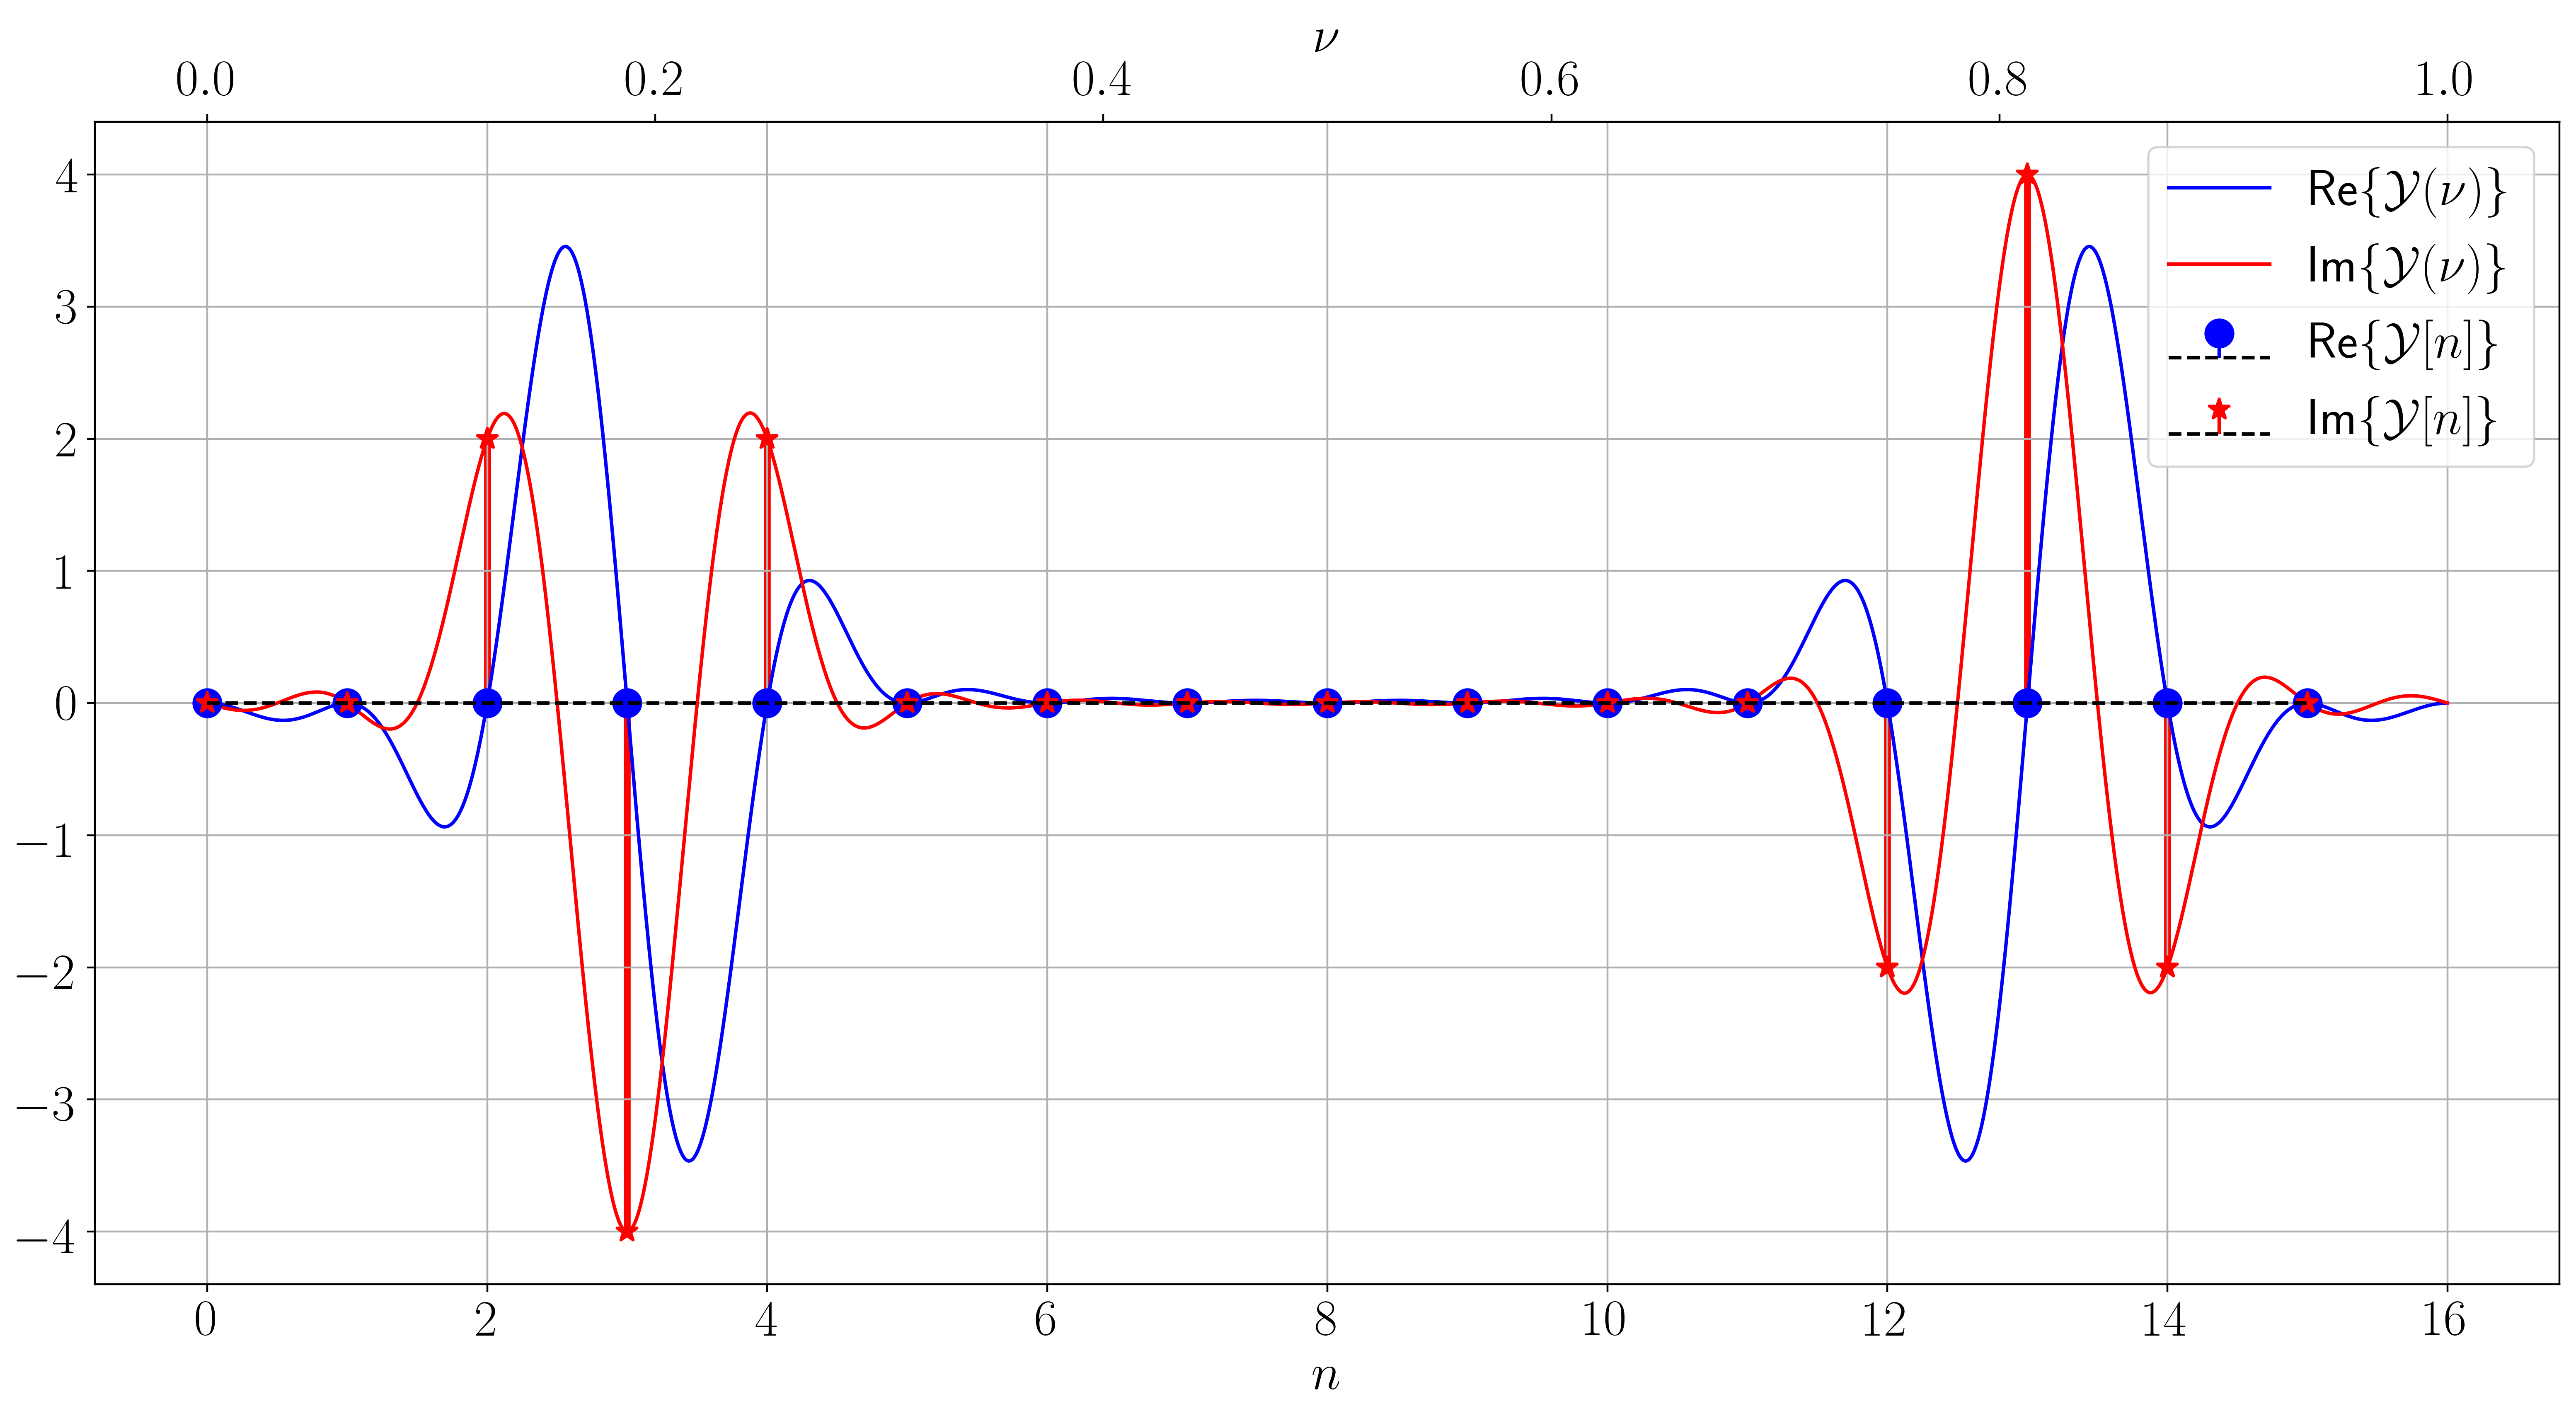
\includegraphics[width=1.\columnwidth]{pics/spring/1/1-3.png}
	%\caption{.}
	\label{fig:1-3}
\end{figure}


\setcounter{chapter}{2}
\setcounter{section}{0}
%\chapter*{Неделя 2}
\protect\thispagestyle{fancy}
\section{}
Даны два сигнала, представленные в виде линейной комбинации двух косинусоид:

\begin{align*}
x_1[k] = \cos( \pi k / 4)  + \cos(17 \pi k / 64),\\
x_2[k] = \cos( \pi k / 4)  + \cos(21 \pi k / 64).
\end{align*}

Вычисляется спектральная оценка каждого из этих сигналов с помощью $64$-точечного ДПФ  и $64$-точечного прямоугольного окна.
Определить, будут ли различимы спектральные максимумы в каждом из двух случаев.

\begin{align*}
x_1[k] &= \cos( \pi k / 4)  + \cos(17 \pi k / 64) = \cos( 8\cdot 2\pi k / 64)  + \cos(8.5 \cdot 2 \pi k / 64).\\
\mathcal{X}_1(\nu) &= \dfrac{1}{2}\left[\mathcal{W}_{\mathcal{D}}\left(\nu-\dfrac{8}{64}\right) +
\mathcal{W}_{\mathcal{D}}\left(\nu+\dfrac{8}{64}\right) +
\mathcal{W}_{\mathcal{D}}\left(\nu-\dfrac{8.5}{64}\right) +
\mathcal{W}_{\mathcal{D}}\left(\nu+\dfrac{8.5}{64}\right)\right]^{\footnotemark}.
\end{align*}
\footnotetext{$\Capit{W}_{\Capit{D}}(\nu) = \dfrac{\sin (N \pi \nu)}{\sin(\pi \nu)}e^{-j(N-1)\pi \nu}$ -- ДВПФ прямоугольного окна (окна Дирихле) из $N=64$ отсчётов.}

Расстояние между относительными частотами косинусоид $\Delta \nu = \frac{8.5-8}{64} = \frac{0.5}{64}$, то есть справедливо, что $\Delta \nu < \frac{0.89}{64} = \Delta \nu_{-3\text{dB}}$. В этом случае можно сделать вывод о том, что спектральные максимумы в ДПФ не будут различимы (сольются в один максимум).


\begin{align*}
x_2[k] &= \cos( \pi k / 4)  + \cos(21 \pi k / 64) = \cos(2\cdot 8\pi k / 64)  + \cos(10.5 \cdot 2 \pi k / 64).\\
\mathcal{X}_2(\nu) &= \dfrac{1}{2}\left[\mathcal{W}_{\mathcal{D}}\left(\nu-\dfrac{8}{64}\right) +
\mathcal{W}_{\mathcal{D}}\left(\nu+\dfrac{8}{64}\right) +
\mathcal{W}_{\mathcal{D}}\left(\nu-\dfrac{10.5}{64}\right) +
\mathcal{W}_{\mathcal{D}}\left(\nu+\dfrac{10.5}{64}\right)\right].
\end{align*}

Расстояние между относительными частотами косинусоид $\Delta \nu = \frac{10.5-8}{64} = \frac{2.5}{64}$, что превышает ширину главного лепестка окна на нулевом уровне $\Delta \nu_0 = \left(\frac{2}{64}\right)$. С учётом того, что абсолютные значения амплитуд максимумов совпадают, можно сделать вывод о том, что спектральные максимумы будут различимы как в ДВПФ, так и в ДПФ.

\begin{figure}[!h]
	\centering
	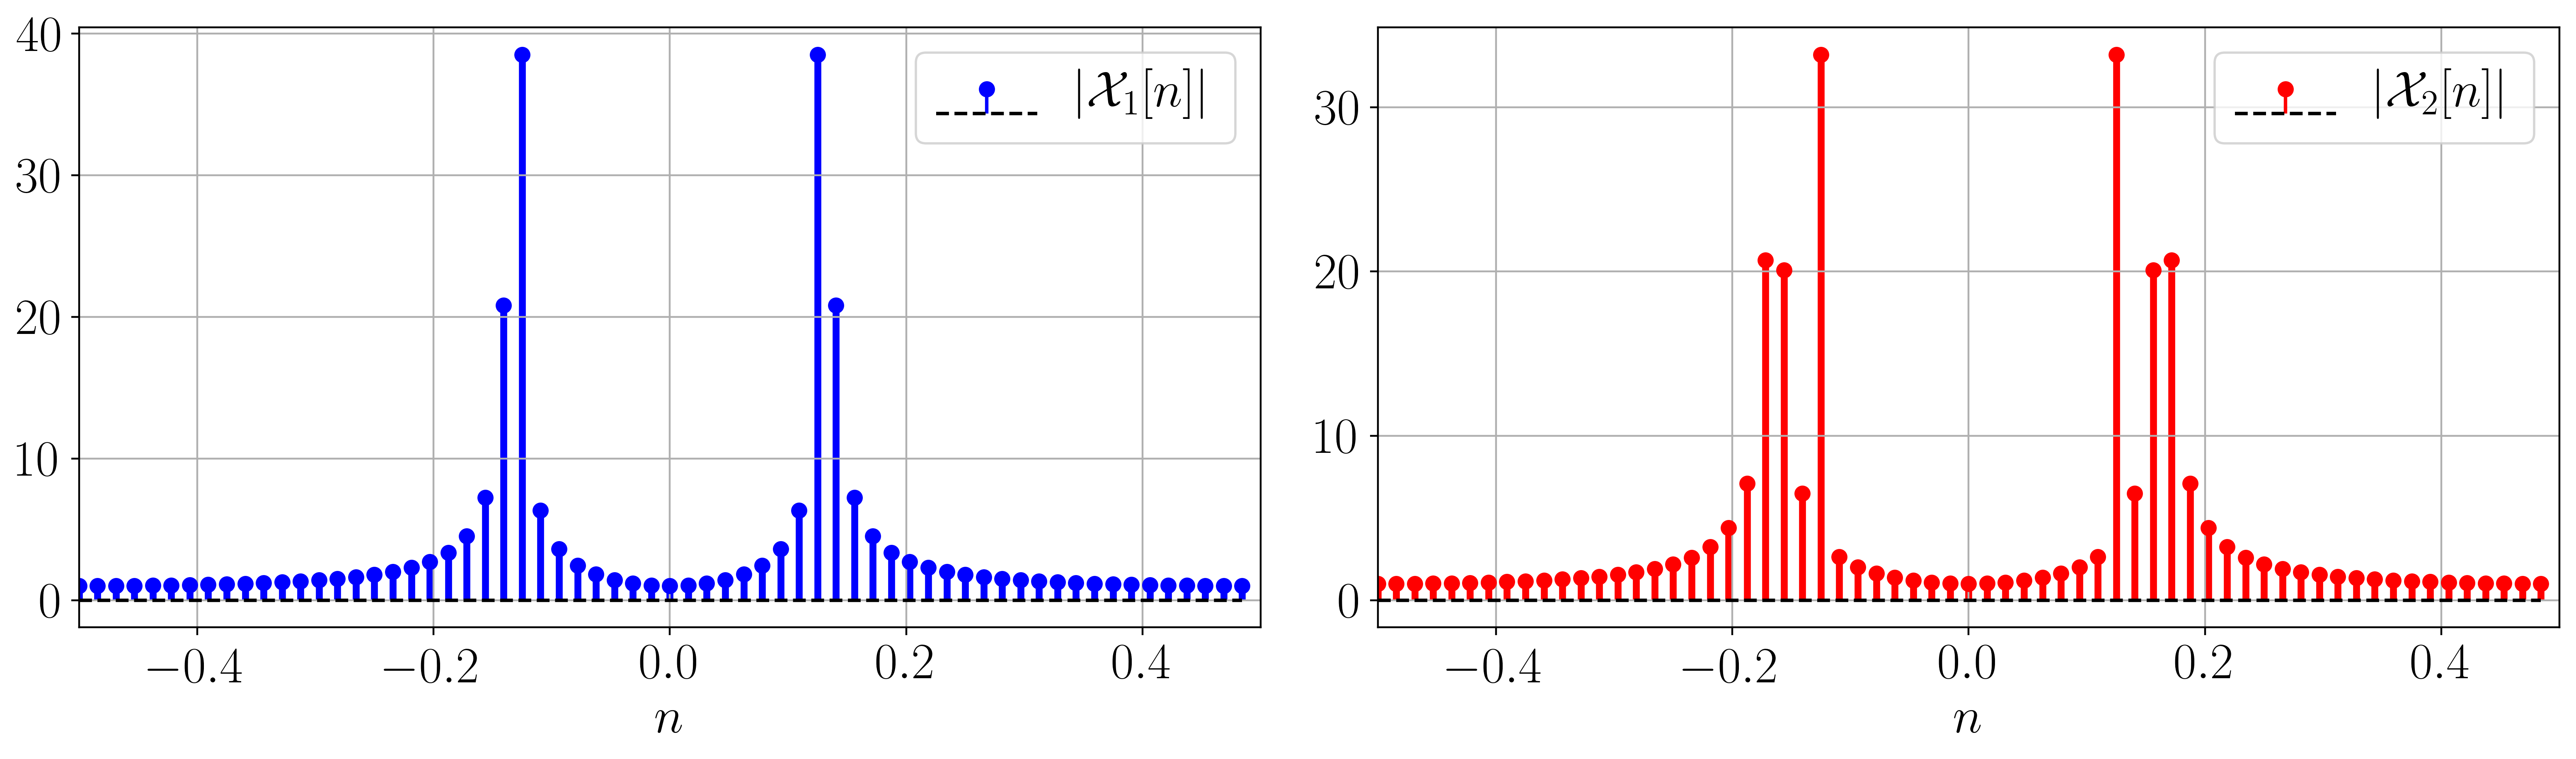
\includegraphics[width=1.\columnwidth]{pics/spring/2/2-1.png}
	%\caption{.}
	\label{fig:2-1}
\end{figure}



\newpage
\section{}
Пусть известно, что обрабатываемая последовательность имеет вид
\begin{equation*}
x[k] = \sum \limits_{m=0}^{M} \mathcal{A}_m \cos\left(2\pi\frac{m}{N}k + \varphi_m \right),\quad k = 0, 1, \ldots, N-1,
\end{equation*}

где $\mathcal{A}_m$ и $\varphi_m$ -- неизвестные заранее амплитуды и фазы гармонических составляющих;
$m$ -- неизвестные заранее целые числа, определяющие нормированные частоты $\nu_m = m/N$ гармонических составляющих, которые совпадают с бинами ДПФ.

Выразите неизвестные амплитуды и фазы через отсчёты ДПФ данной последовательности.

\begin{align*}
\mathcal{X}[n] &= \sum \limits_{k=0}^{N-1}x[k]e^{-j2\pi\frac{nk}{N}} = 
\sum \limits_{k=0}^{N-1} \left(\sum \limits_{m=0}^{M} \mathcal{A}_m \cos\left(2\pi\frac{m}{N}k + \varphi_m \right)\right) e^{-j2\pi\frac{nk}{N}} = \\
&= \dfrac{1}{2} \sum \limits_{m=0}^{M} \mathcal{A}_m
\sum \limits_{k=0}^{N-1} \left( e^{j(2\pi\frac{m}{N}k + \varphi_m)} + e^{-j(2\pi\frac{m}{N}k + \varphi_m)} \right) e^{-j2\pi\frac{nk}{N}} = \\
&= \dfrac{1}{2} \sum \limits_{m=0}^{M} \mathcal{A}_m \left( 
\sum \limits_{k=0}^{N-1}  e^{j(2\pi\frac{m-n}{N}k + \varphi_m)}
+  \sum \limits_{k=0}^{N-1}  e^{-j(2\pi\frac{m+n}{N}k + \varphi_m)}
\right) = \\
&= \dfrac{1}{2} \sum \limits_{m=0}^{M} \mathcal{A}_m \left( 
e^{+j\varphi_m}\sum \limits_{k=0}^{N-1}  e^{j2\pi\frac{m-n}{N}k}
+  e^{-j\varphi_m}\sum \limits_{k=0}^{N-1}  e^{j2\pi\frac{N-(m+n)}{N}k}
\right) = \\
&= \dfrac{N}{2} \sum \limits_{m=0}^{M} \mathcal{A}_m \left( 
e^{+j\varphi_m}\delta_{m, n}
+  e^{-j\varphi_m}\delta_{m, N - n}
\right) = \dfrac{N}{2} \left(\mathcal{A}_ne^{+j\varphi_n} + \mathcal{A}_{N-n}e^{-j\varphi_{N-n}}\right).
\end{align*}

Если $M \leq \lceil N/2 \rceil - 1$, то система уравнений будет однозначно и легко разрешима относительно неизвестных $\mathcal{A}_m$ и $\varphi_m$:

\begin{equation*}
\mathcal{A}_{m} = \dfrac{2}{N}|\mathcal{X}[m]|, \quad \varphi_m = \arg\{X[m]\}, \quad m=0, \ldots, M \leq \lceil N/2 \rceil - 1.
\end{equation*}

\section{}
Предположим, что нужно вычислить спектральную оценку дискретного сигнала с помощью ДВПФ и окна. При этом необходимо добиться разрешения не менее $\Delta \nu = 0.0075$, а длина окна фиксирована и равна $N = 256$. 

Используя данные из таблицы приложения к лекции, определить, какие из следующих окон гарантированно позволяют выполнить поставленную задачу:
а) прямоугольное,	б) Бартлета,	в) Ханна,\\	г) Хэмминга,	д) Блэкмана.

Заметим, что $\Delta \nu = 0.0075 = \frac{1.92}{N}$. Спектральные компоненты будут гарантировано различимы, если $\Delta \nu = \frac{1.92}{N} \geq \Delta \nu_{-6\text{dB}}$. Исходя из этого условия, заключаем, что для задачи подходят: 
а) прямоугольное окно $\left(\Delta \nu_{-6\text{dB}} = \frac{1.2}{N}\right)$,
б) окно Бартлета $\left(\Delta \nu_{-6\text{dB}} = \frac{1.78}{N}\right)$, 
г) окно Хэмминга $\left(\Delta \nu_{-6\text{dB}} = \frac{1.82}{N}\right)$.


\setcounter{chapter}{3}
\setcounter{section}{0}
%\chapter*{Неделя 3}
\protect\thispagestyle{fancy}
\section{}
Изобразить граф алгоритма БПФ с прореживанием \textbf{по частоте} для $N=16$. 
Объяснить, в чем заключается базовая операция данного алгоритма.

\begin{figure}[!h]
	\centering
	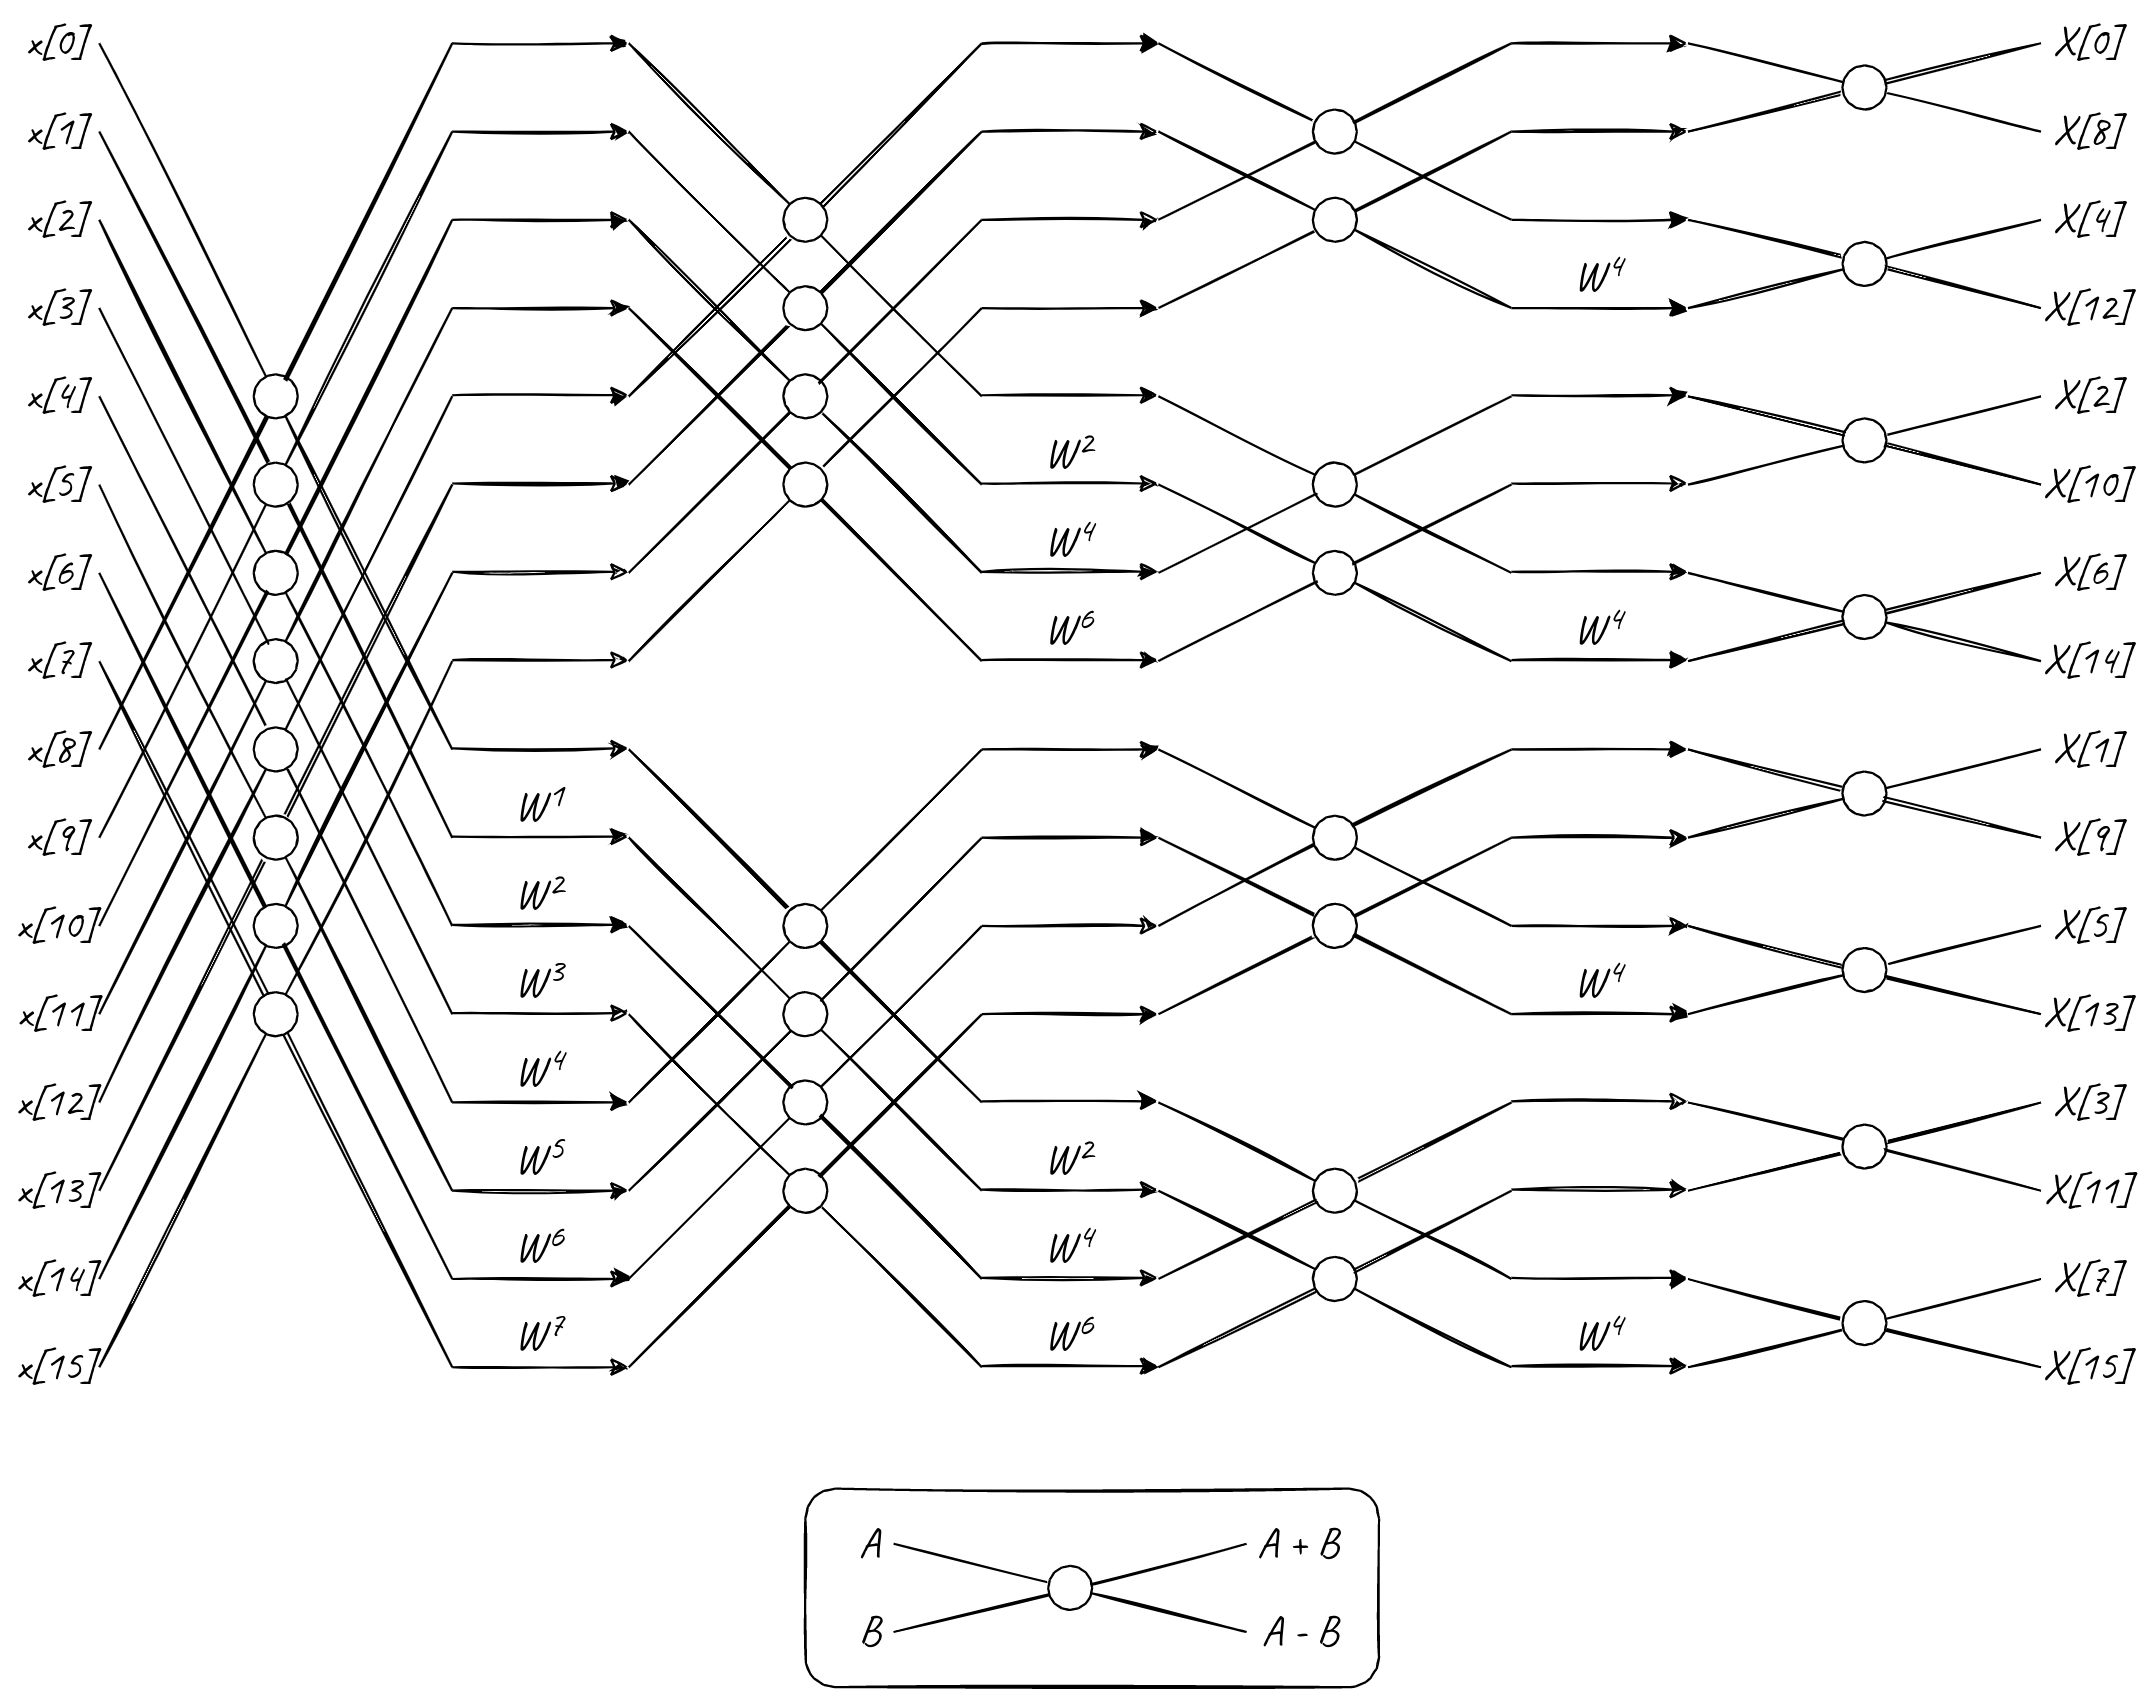
\includegraphics[width=1.\columnwidth]{pics/spring/3/1.png}
	%\caption{.}
	\label{fig:3-1}
\end{figure}

Базовой операцией является двухточечное ДПФ по основанию $2$, состоящее из сложения и вычитания и не содержащее умножений. Все умножения вынесены в поворачивающие множители между итерациями алгоритма. Входные отсчеты должны быть расположены в естественном битовом порядке, а выходные --- в инверсном битовом порядке.

\newpage
\section{}
Изобразить граф алгоритма БПФ с прореживанием \textbf{по времени} для $N=16$. 
Объяснить, в чем заключается базовая операция данного алгоритма.
\begin{figure}[!h]
	\centering
	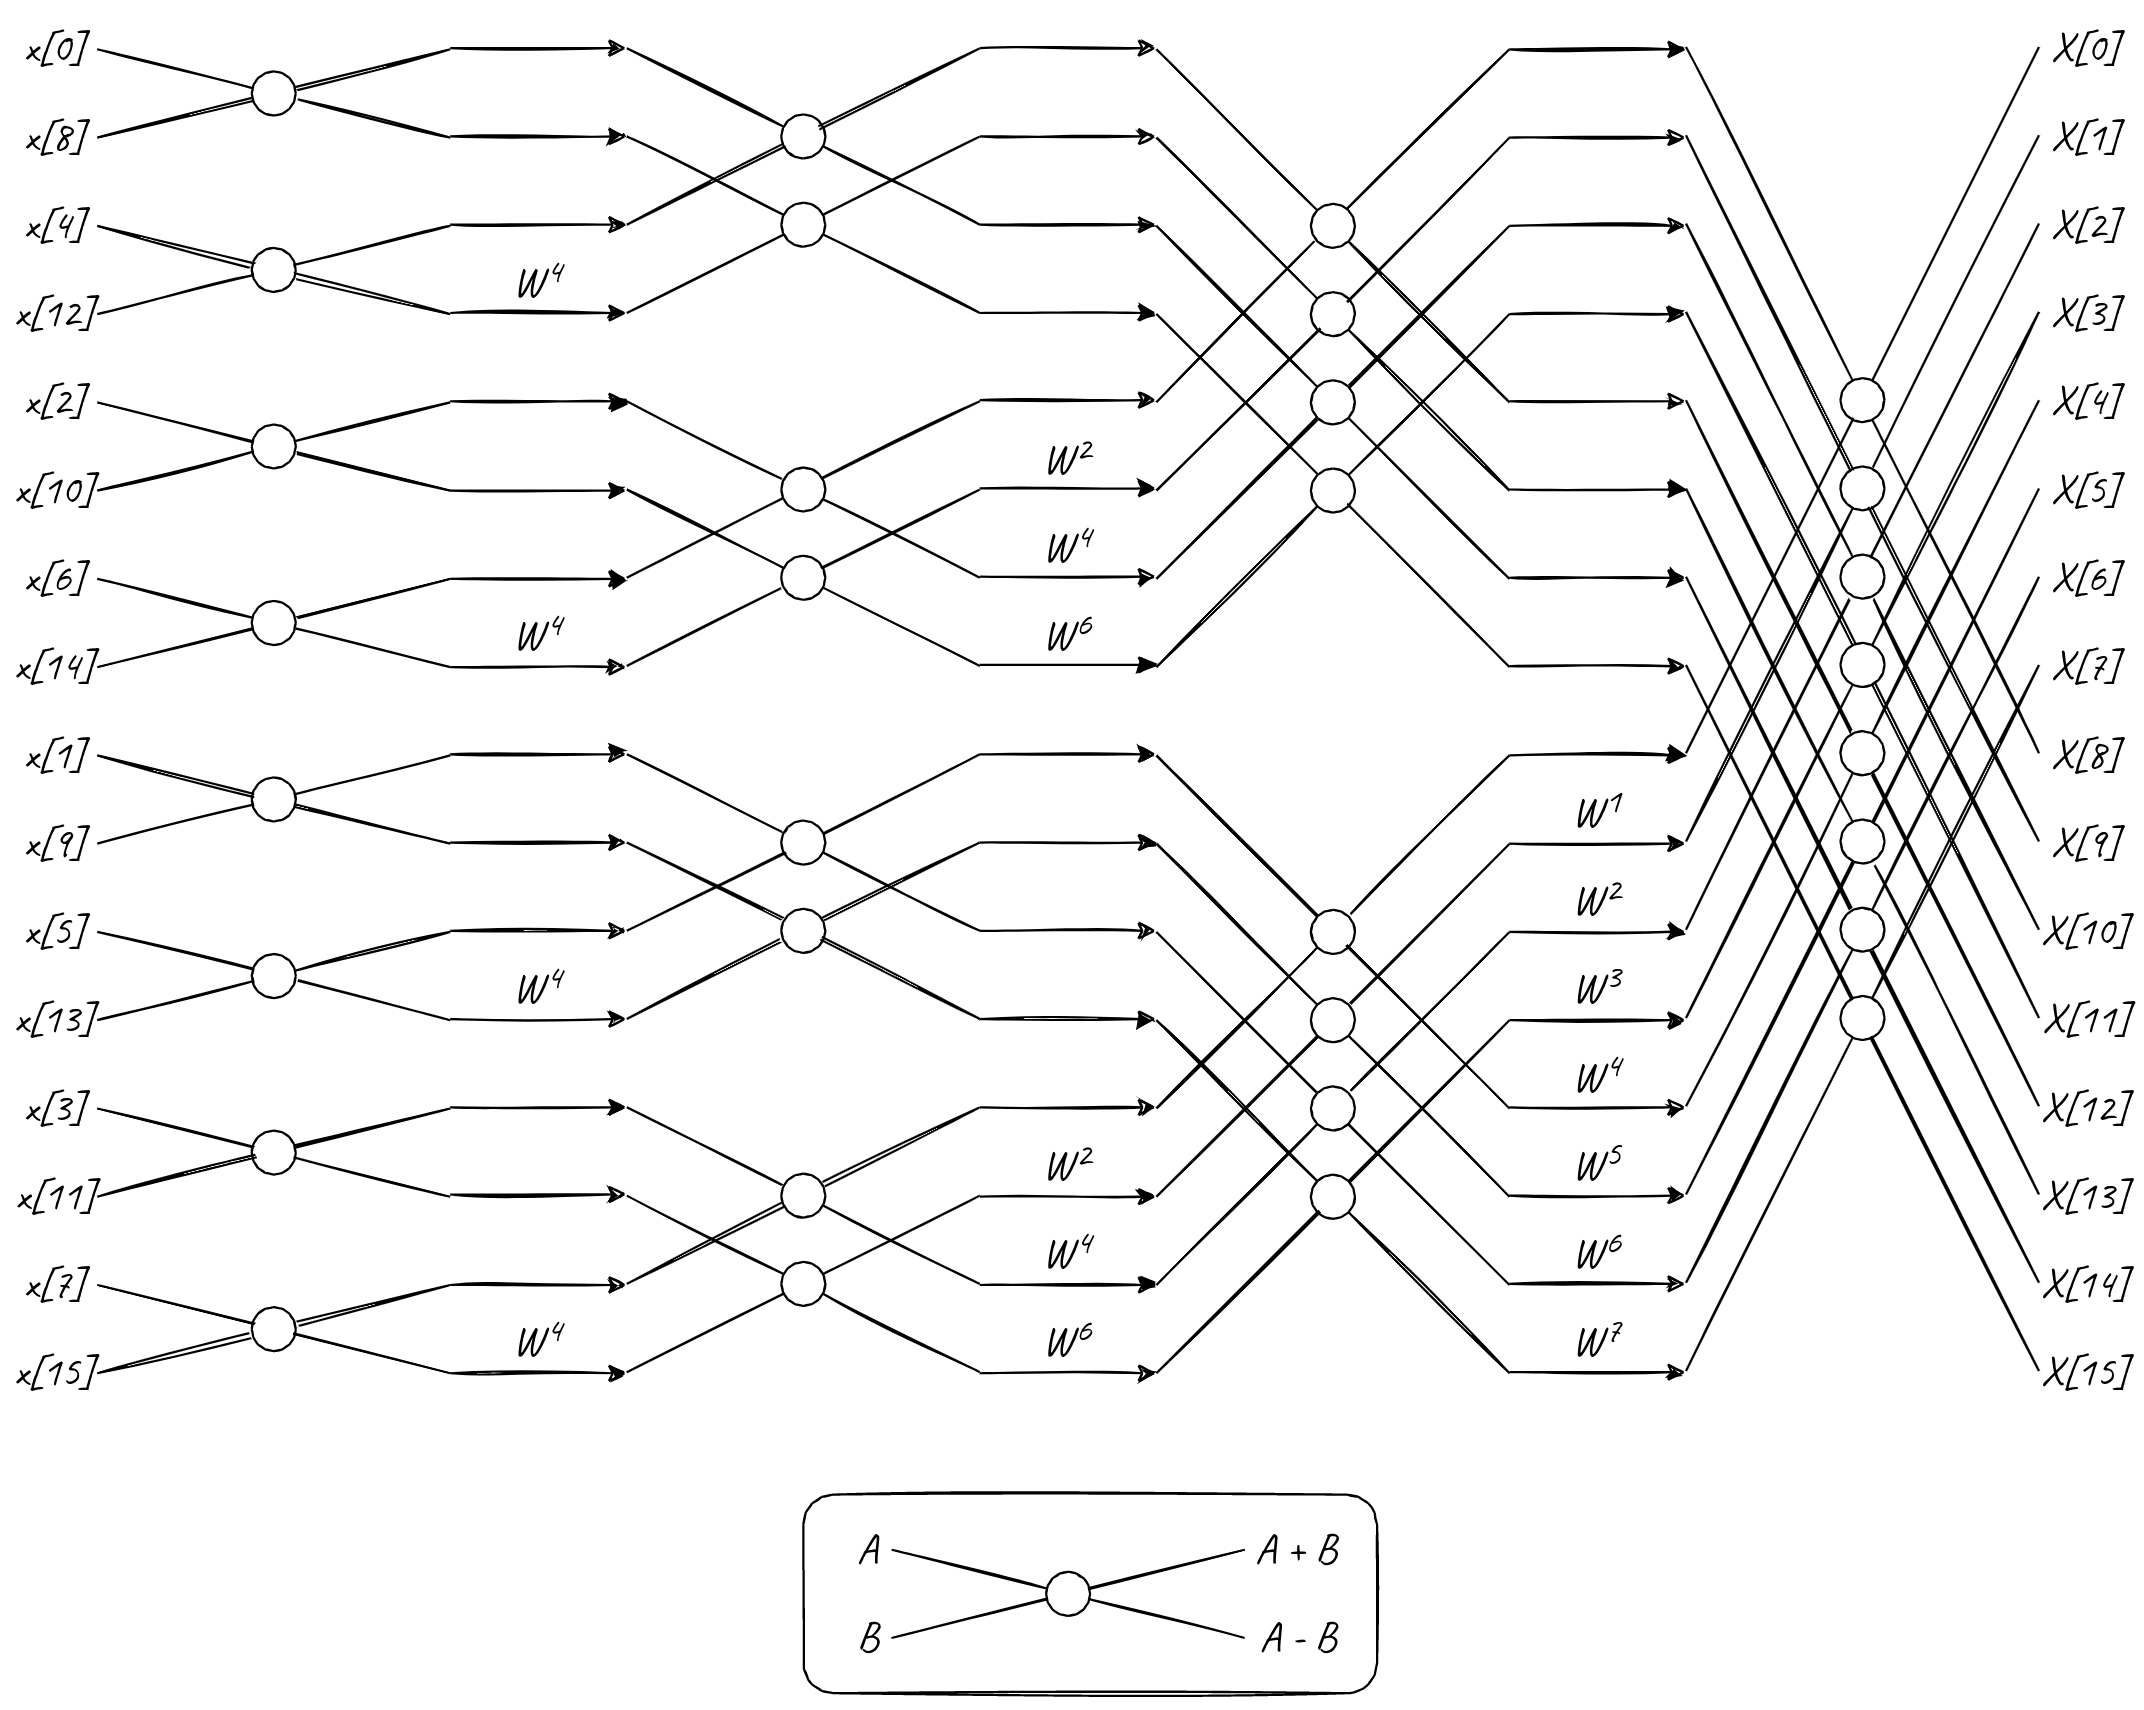
\includegraphics[width=1.\columnwidth]{pics/spring/3/2.png}
	%\caption{.}
	\label{fig:3-2}
\end{figure}

Базовой операцией является двухточечное ДПФ по основанию $2$, состоящее из сложения и вычитания и не содержащее умножений. Все умножения вынесены в поворачивающие множители между итерациями алгоритма. Входные отсчеты должны быть расположены в инверсном битовом порядке, а выходные --- в естественном битовом порядке.



\newpage
\section{}
Записать матрицу, задающую ДПФ преобразование над последовательностью (вектором) длины $4$. Указать матрицу, задающую обратное преобразование. 
В ответе значения всех элементов матрицы должны быть представлены как комплексные числа.

\begin{equation*}
[W_4] =
\begin{bmatrix}
W^0_4 & W^0_4 & W^0_4 & W^0_4\\
W^0_4 & W^1_4 & W^2_4 & W^3_4\\
W^0_4 & W^2_4 & W^4_4 & W^6_4\\
W^0_4 & W^3_4 & W^6_4 & W^9_4
\end{bmatrix} =
\begin{bmatrix}
W^0_4 & W^0_4 & W^0_4 & W^0_4\\
W^0_4 & W^1_4 & W^2_4 & W^3_4\\
W^0_4 & W^2_4 & W^0_4 & W^2_4\\
W^0_4 & W^3_4 & W^2_4 & W^1_4
\end{bmatrix} =
\begin{bmatrix}
+1 & +1 & +1 & +1\\
+1 & -j & -1 & +j\\
+1 & -1 & +1 & -1\\
+1 & +j & -1 & -j
\end{bmatrix}.
\end{equation*}

\begin{equation*}
[W_4]^{-1} = \dfrac{1}{4}[W_4]^{*} = \dfrac{1}{4}
\begin{bmatrix}
+1 & +1 & +1 & +1\\
+1 & +j & -1 & -j\\
+1 & -1 & +1 & -1\\
+1 & -j & -1 & +j
\end{bmatrix}.
\end{equation*}


\setcounter{chapter}{4}
\setcounter{section}{0}
%\chapter*{Неделя 4}
\protect\thispagestyle{fancy}
\section{}
Предположим, что требуется найти $7$-ой отчет $8$-точечного ДПФ некоторой действительной последовательности. 
Сравнить (заполнить таблицу) количество операций, которое требуется для вычисления $8$-точечного ДПФ по алгоритму БПФ с прореживанием по частоте с числом операций в алгоритме Герцеля.


\begin{center}
	\begin{tabular}{||c|| c | c | c||} 
		\hline
		& БПФ & БПФ ($\mathcal{X}[7]$) & Алгоритм Герцеля ($\mathcal{X}[7]$) \\ [0.5ex] 
		\hline\hline
		\color{teal}{Число действительных сложений и вычитаний} & $14$ & $4$ & $16$ \\ 
		\hline
		\color{orange}{Число действительных умножений} & $0(3)$ & $0(2)$ & $8$ \\
		\hline
		\color{red}{Число комплексных сложений и вычитаний} & $10$ & $3$ & $1$ \\
		\hline
		\color{blue}{Число комплексных умножений} & $5(2)$ & $4(2)$ & $1$ \\
		\hline
	\end{tabular}
\end{center}

Для алгоритма БПФ с прореживанием по частоте найдём общее число операций в графе, которое потребуется, чтобы посчитать весь вектор ДПФ. Также найдём число операций, которое нужно, чтобы найти только один отсчёт $X[7]$. Вo втором случае для наглядности операции выделены в графе соответствующими цветами. Значения в скобках учитывают, что умножение на чисто мнимое число $W^2 = W^2_8 = \exp(-j2\pi\frac{2}{8}) = -j$ в некотором смысле можно считать действительным умножением внутри мнимой части комплексного числа.

\begin{figure}[!h]
	\centering
	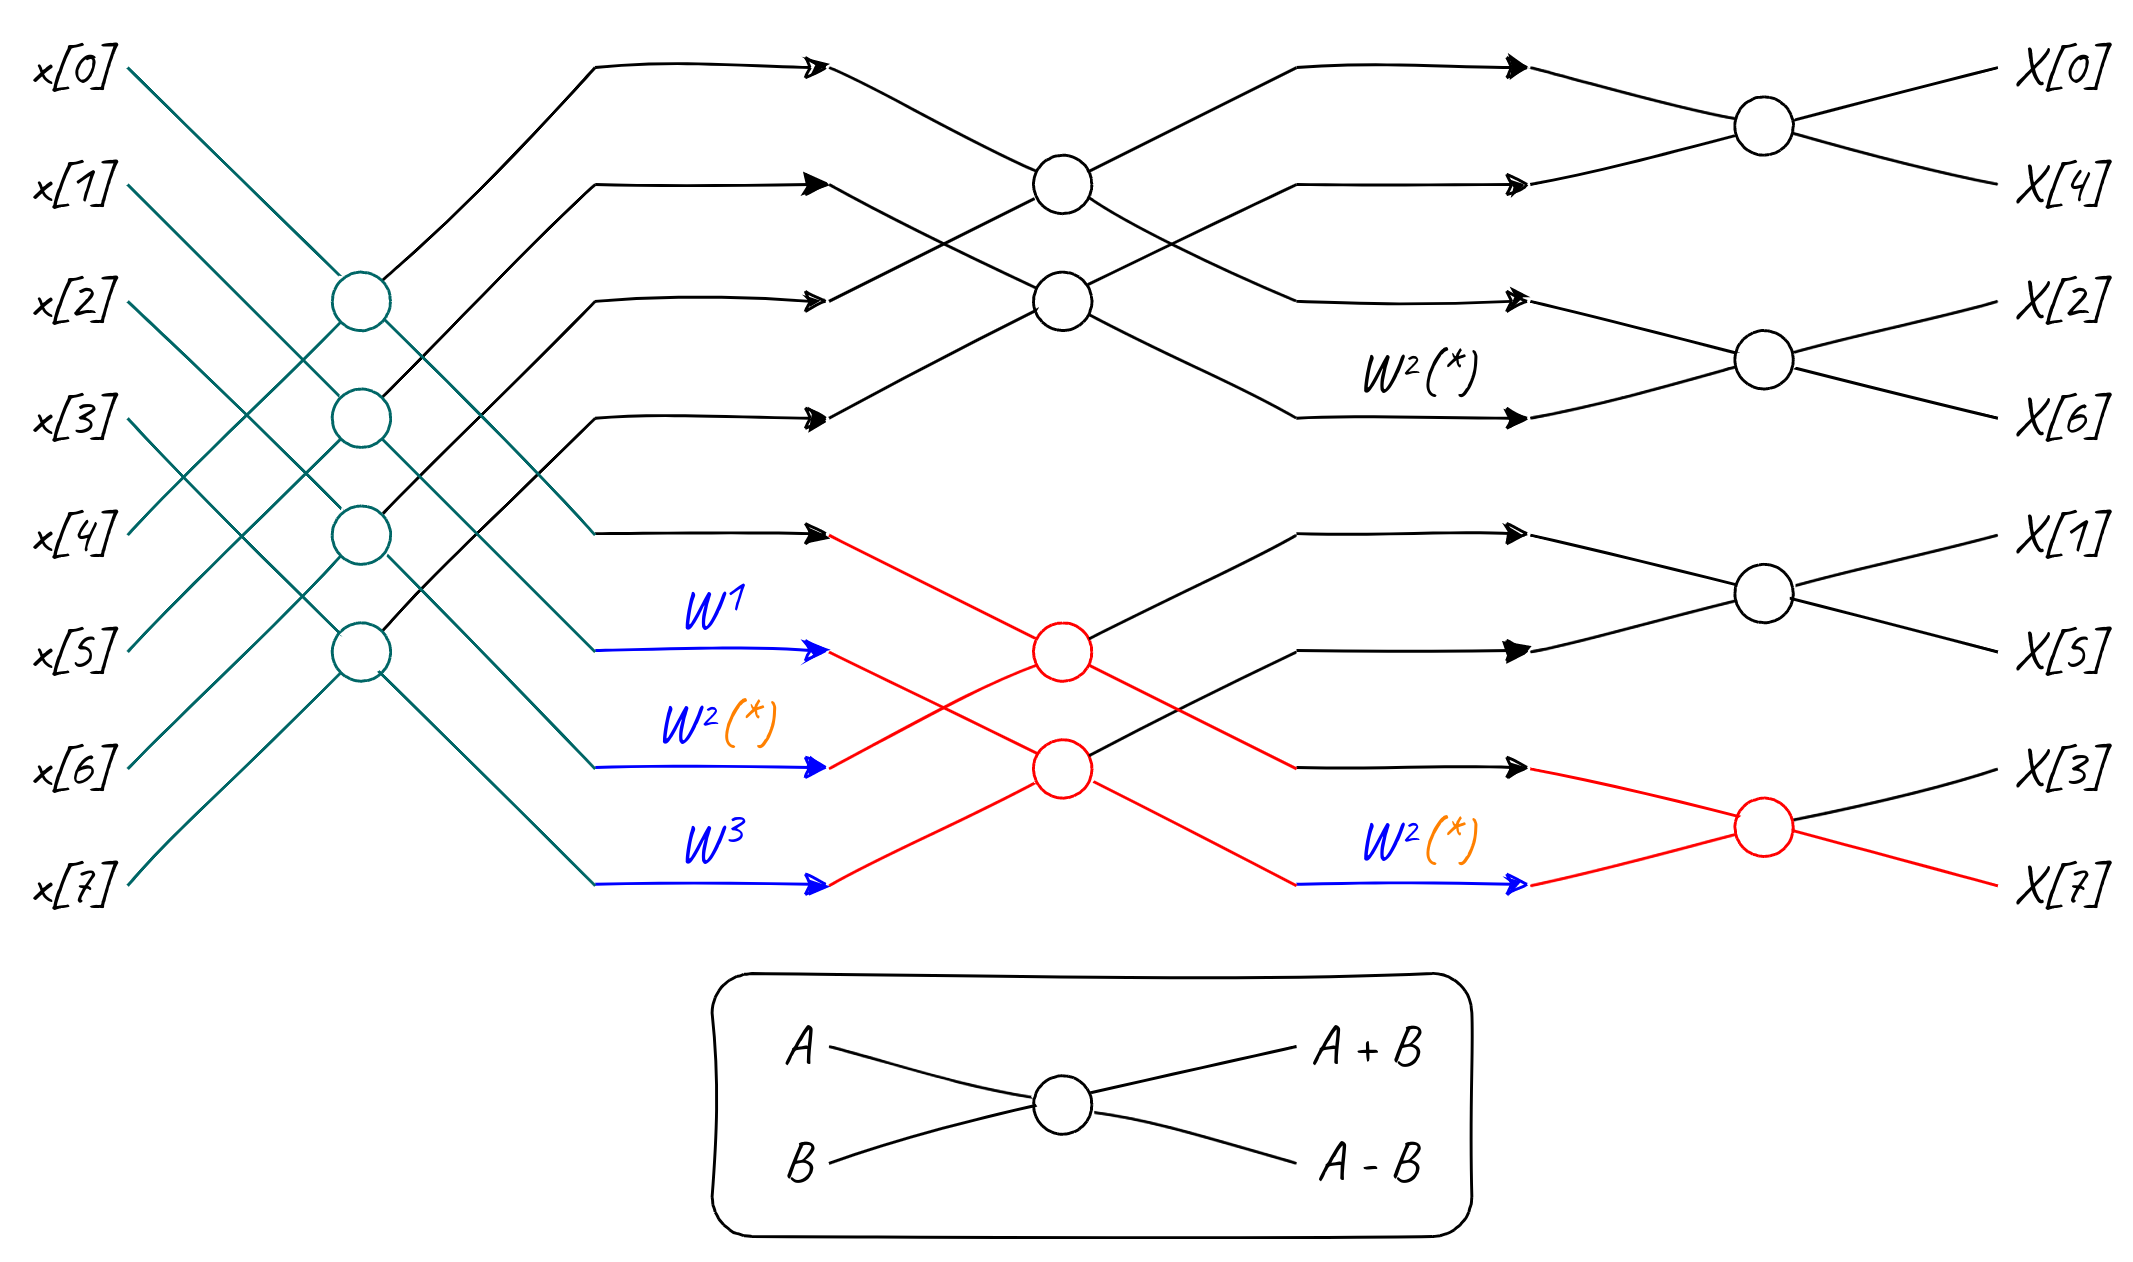
\includegraphics[width=1.\columnwidth]{pics/spring/4/1.png}
	%\caption{.}
	\label{fig:4-1}
\end{figure}

Для поиска $\mathcal{X}[7]$ согласно алгоритму Герцеля будем иметь следующие соотношения. Знаки арифметических операций выделены соответствующими цветами.
\begin{align*}
&\mathcal{V}_7[m] = x[m] \color{teal}+\color{black} 2\cos\left(2\pi \dfrac{7}{8}\right)  \color{orange}\times\color{black} \mathcal{V}_7[m-1] \color{teal}-\color{black} \mathcal{V}_7[m-2],\quad 0\leq m \leq 7,\\
&\mathcal{X}[7] = W^{-7}_8 \color{blue}\times\color{black} V_7[7] \color{red}-\color{black} V_7[6].
\end{align*}


\newpage
\section{}
Пусть требуется вычислить $3$-ий отсчет $64$-точечного ДПФ некоторой действительной последовательности конечной длительности.

Привести блок-схемы фильтров:
\begin{enumerate}[label=(\alph*)]
	\item БИХ-фильтра второго порядка алгоритма Герцеля,
	\item рекурсивного КИХ-фильтра скользящего спектрального анализа.
\end{enumerate}
Указать, как выход фильтра соответствует значению искомого отсчета ДПФ.


\begin{enumerate}[label=(\alph*)]
	\item Схема БИХ-фильтра второго порядка алгоритма Герцеля для поиска $3$-ого отсчета $64$-точечного ДПФ действительной последовательности конечной длительности изображена на рис.~\ref{fig:4-2-1}. При этом правую часть фильтра (в красной рамке) достаточно вычислить лишь один раз на финальном этапе. Искомый отсчёт ДПФ будет равен выходу фильтра (с правой частью) на последней $63$-ей итерации (считая с нулевой).
	
	\begin{figure}[!h]
		\centering
		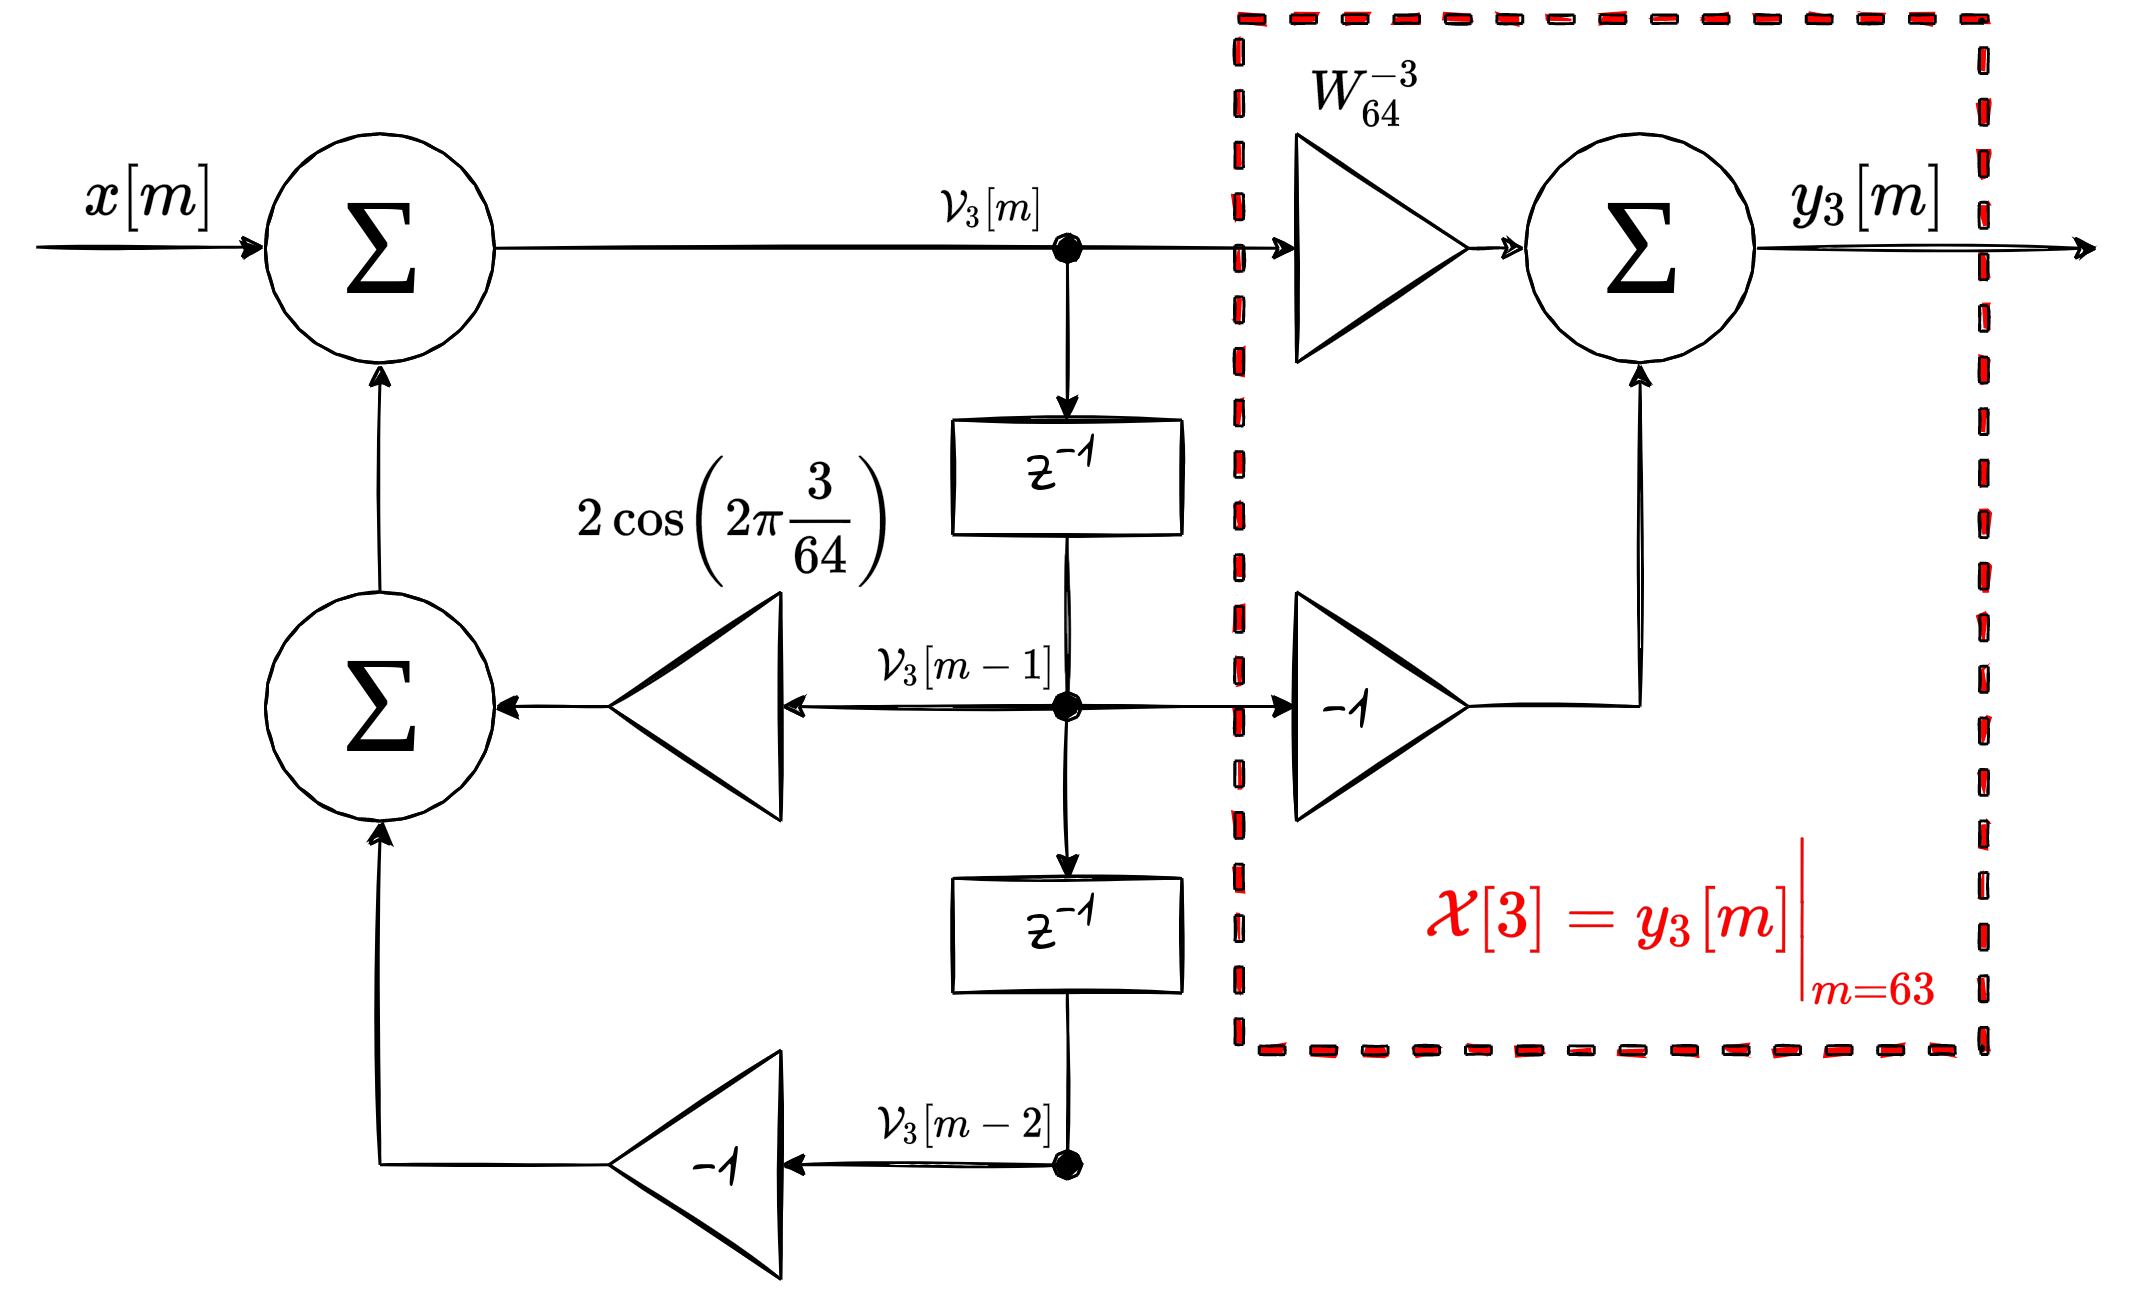
\includegraphics[width=0.65\columnwidth]{pics/spring/4/2-1.png}
		\caption{Схема БИХ-фильтра второго порядка алгоритма Герцеля.}
		\label{fig:4-2-1}
	\end{figure}
	
	
	\item На рис.~\ref{fig:4-2-2} представлена схема рекурсивного КИХ-фильтра скользящего однобинового спектрального анализа для поиска $3$-ого отсчета $64$-точечного ДПФ действительной последовательности конечной длительности.
	Искомый отсчёт ДПФ будет равен выходу фильтра на $63$-ей итерации алгоритма (считая с нулевой).
	\begin{figure}[!h]
		\centering
		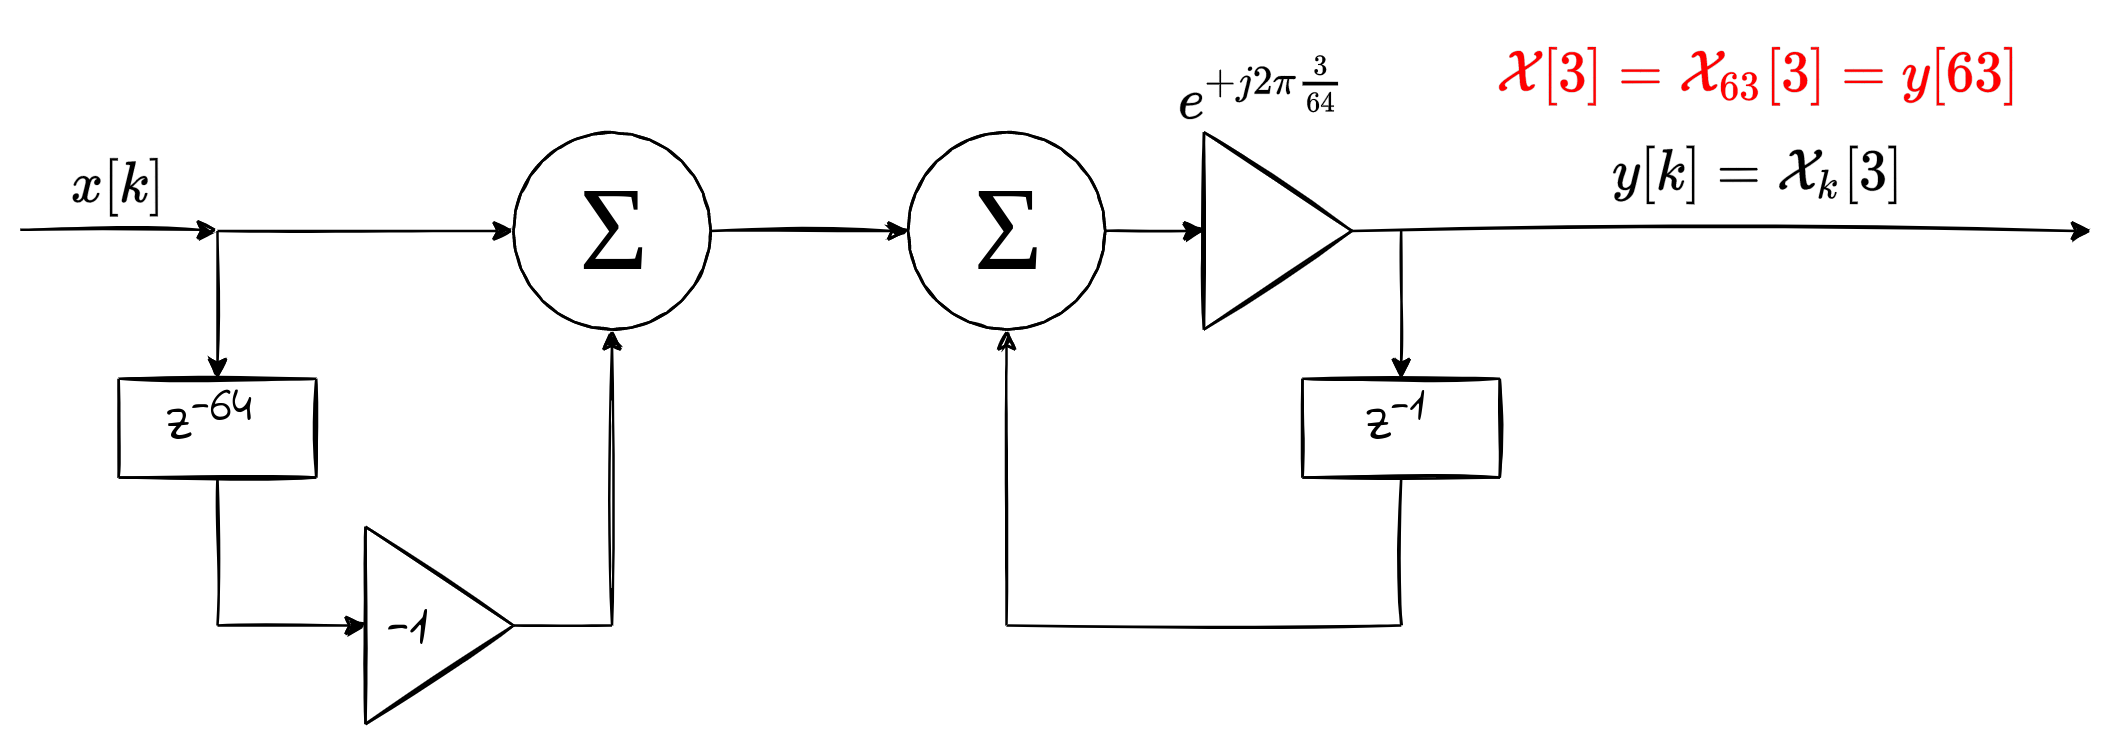
\includegraphics[width=0.65\columnwidth]{pics/spring/4/2-2.png}
		\caption{Схема рекурсивного КИХ-фильтра скользящего однобинового спектрального анализа.}
		\label{fig:4-2-2}
	\end{figure}
	
\end{enumerate}


\newpage
\section{}
Предположим, что с помощью окна длиной $M = 4000$ осуществляется вычисление кратковременного дискретного преобразования Фурье последовательности

\begin{equation*}
x[k] = \cos\left(2\pi\dfrac{f_1}{f_d}k + \varphi_1\right) +
\cos\left(2\pi\dfrac{f_2}{f_d}k + \varphi_2\right)
\end{equation*}

длиной в $N = 40000$ отсчетов без перекрытия. Фазы $\varphi_1$ и $\varphi_2$ неизвестны. Частота дискретизации $f_d = 44100 $ Hz.

Для случая окна Ханна указать, начиная с какого значения $\Delta f = |f_1 - f_2|$ можно выбором необходимой размерности ДПФ $N_{\text{FFT}}$ обеспечить различимость гармонических компонент на спектрограмме.

Спектральные компоненты будут гарантировано различимы, если $\Delta f = |f_1 - f_2| \geq \Delta f_{-6\text{dB}}$.

\begin{equation*}
\Delta f = |f_1 - f_2| \geq \Delta f_{-6\text{dB}} = f_d \cdot \max \left\{\Delta \nu_{-6\text{dB}}, \dfrac{2}{N_{\text{FFT}}}\right\} =
f_d \cdot \max\left\{\dfrac{2.0}{M}, \dfrac{2}{N_{\text{FFT}}}\right\} = \dfrac{2f_d}{M} = 22.05\text{ Hz}.
\end{equation*}


\setcounter{chapter}{5}
\setcounter{section}{0}
%\chapter*{Неделя 5}
\protect\thispagestyle{fancy}
\section{}
Для узкополосного случайного процесса со спектром шириной $\Delta \omega$ сосредоточенным возле частот $\pm \omega_0$ определить и изобразить корреляционную функцию $\Capit{R}(\tau)$.

\begin{figure}[!h]
	\centering
	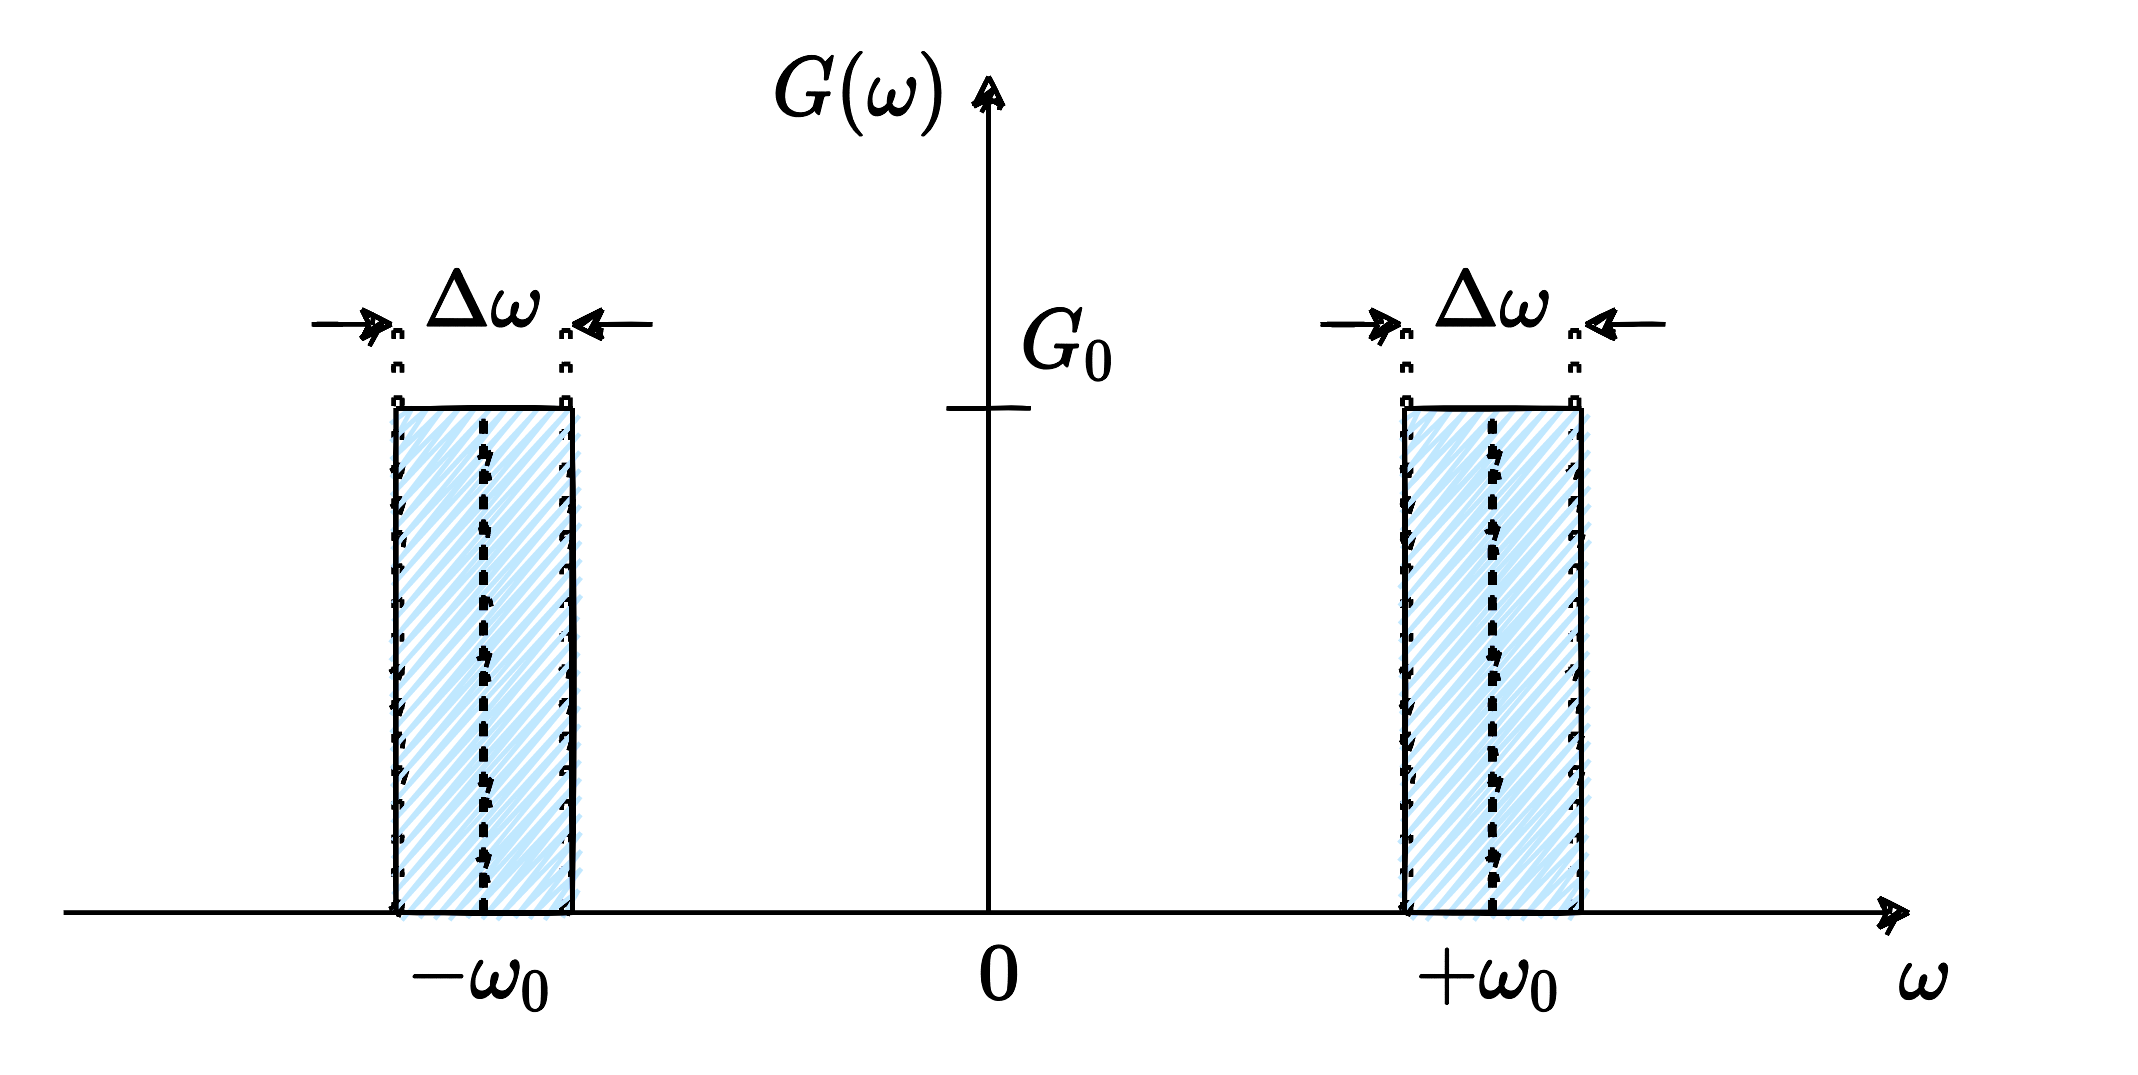
\includegraphics[width=0.65\columnwidth]{pics/spring/5/1-0.png}
	%\caption{.}
	\label{fig:5-1-0}
\end{figure}


\begin{align*}
\Capit{R}(\tau) &= \dfrac{1}{2\pi}\int \limits_{-\infty}^{+\infty} G(\omega)e^{j\omega \tau}d\omega =
\dfrac{1}{\pi}\int \limits_{0}^{+\infty} G(\omega)\cos(\omega \tau)d\omega =
\dfrac{1}{\pi}\int \limits_{\omega_0 - \Delta \omega/2}^{\omega_0 + \Delta \omega/2} G_0\cos(\omega \tau)d\omega =
\dfrac{G_0}{\pi\tau}\int \limits_{\omega_0 - \Delta \omega/2}^{\omega_0 + \Delta \omega/2}d\sin(\omega \tau) = \\ &=
\dfrac{G_0}{\pi\tau} \sin(\omega \tau) \Bigg|_{\omega_0 - \Delta \omega/2}^{\omega_0 + \Delta \omega/2}=
\dfrac{G_0}{\pi\tau} \big[ \sin((\omega_0 + \Delta \omega/2)\tau) - \sin((\omega_0 - \Delta \omega/2)\tau)\big] = 
\dfrac{2G_0}{\pi\tau} \cos (\omega_0 \tau) \sin\left(\dfrac{\Delta \omega \tau}{2}\right) =\\&=
\dfrac{\Delta \omega G_0}{\pi} \cos (\omega_0 \tau) \cdot \dfrac{\sin\left(\dfrac{\Delta \omega \tau}{2}\right)}{\dfrac{\Delta \omega\tau}{2}} =
\dfrac{\Delta \omega G_0}{\pi} \cos (\omega_0 \tau)\cdot \sinc\left(\dfrac{\Delta \omega \tau}{2}\right).
\end{align*}



\begin{figure}[!h]
	\centering
	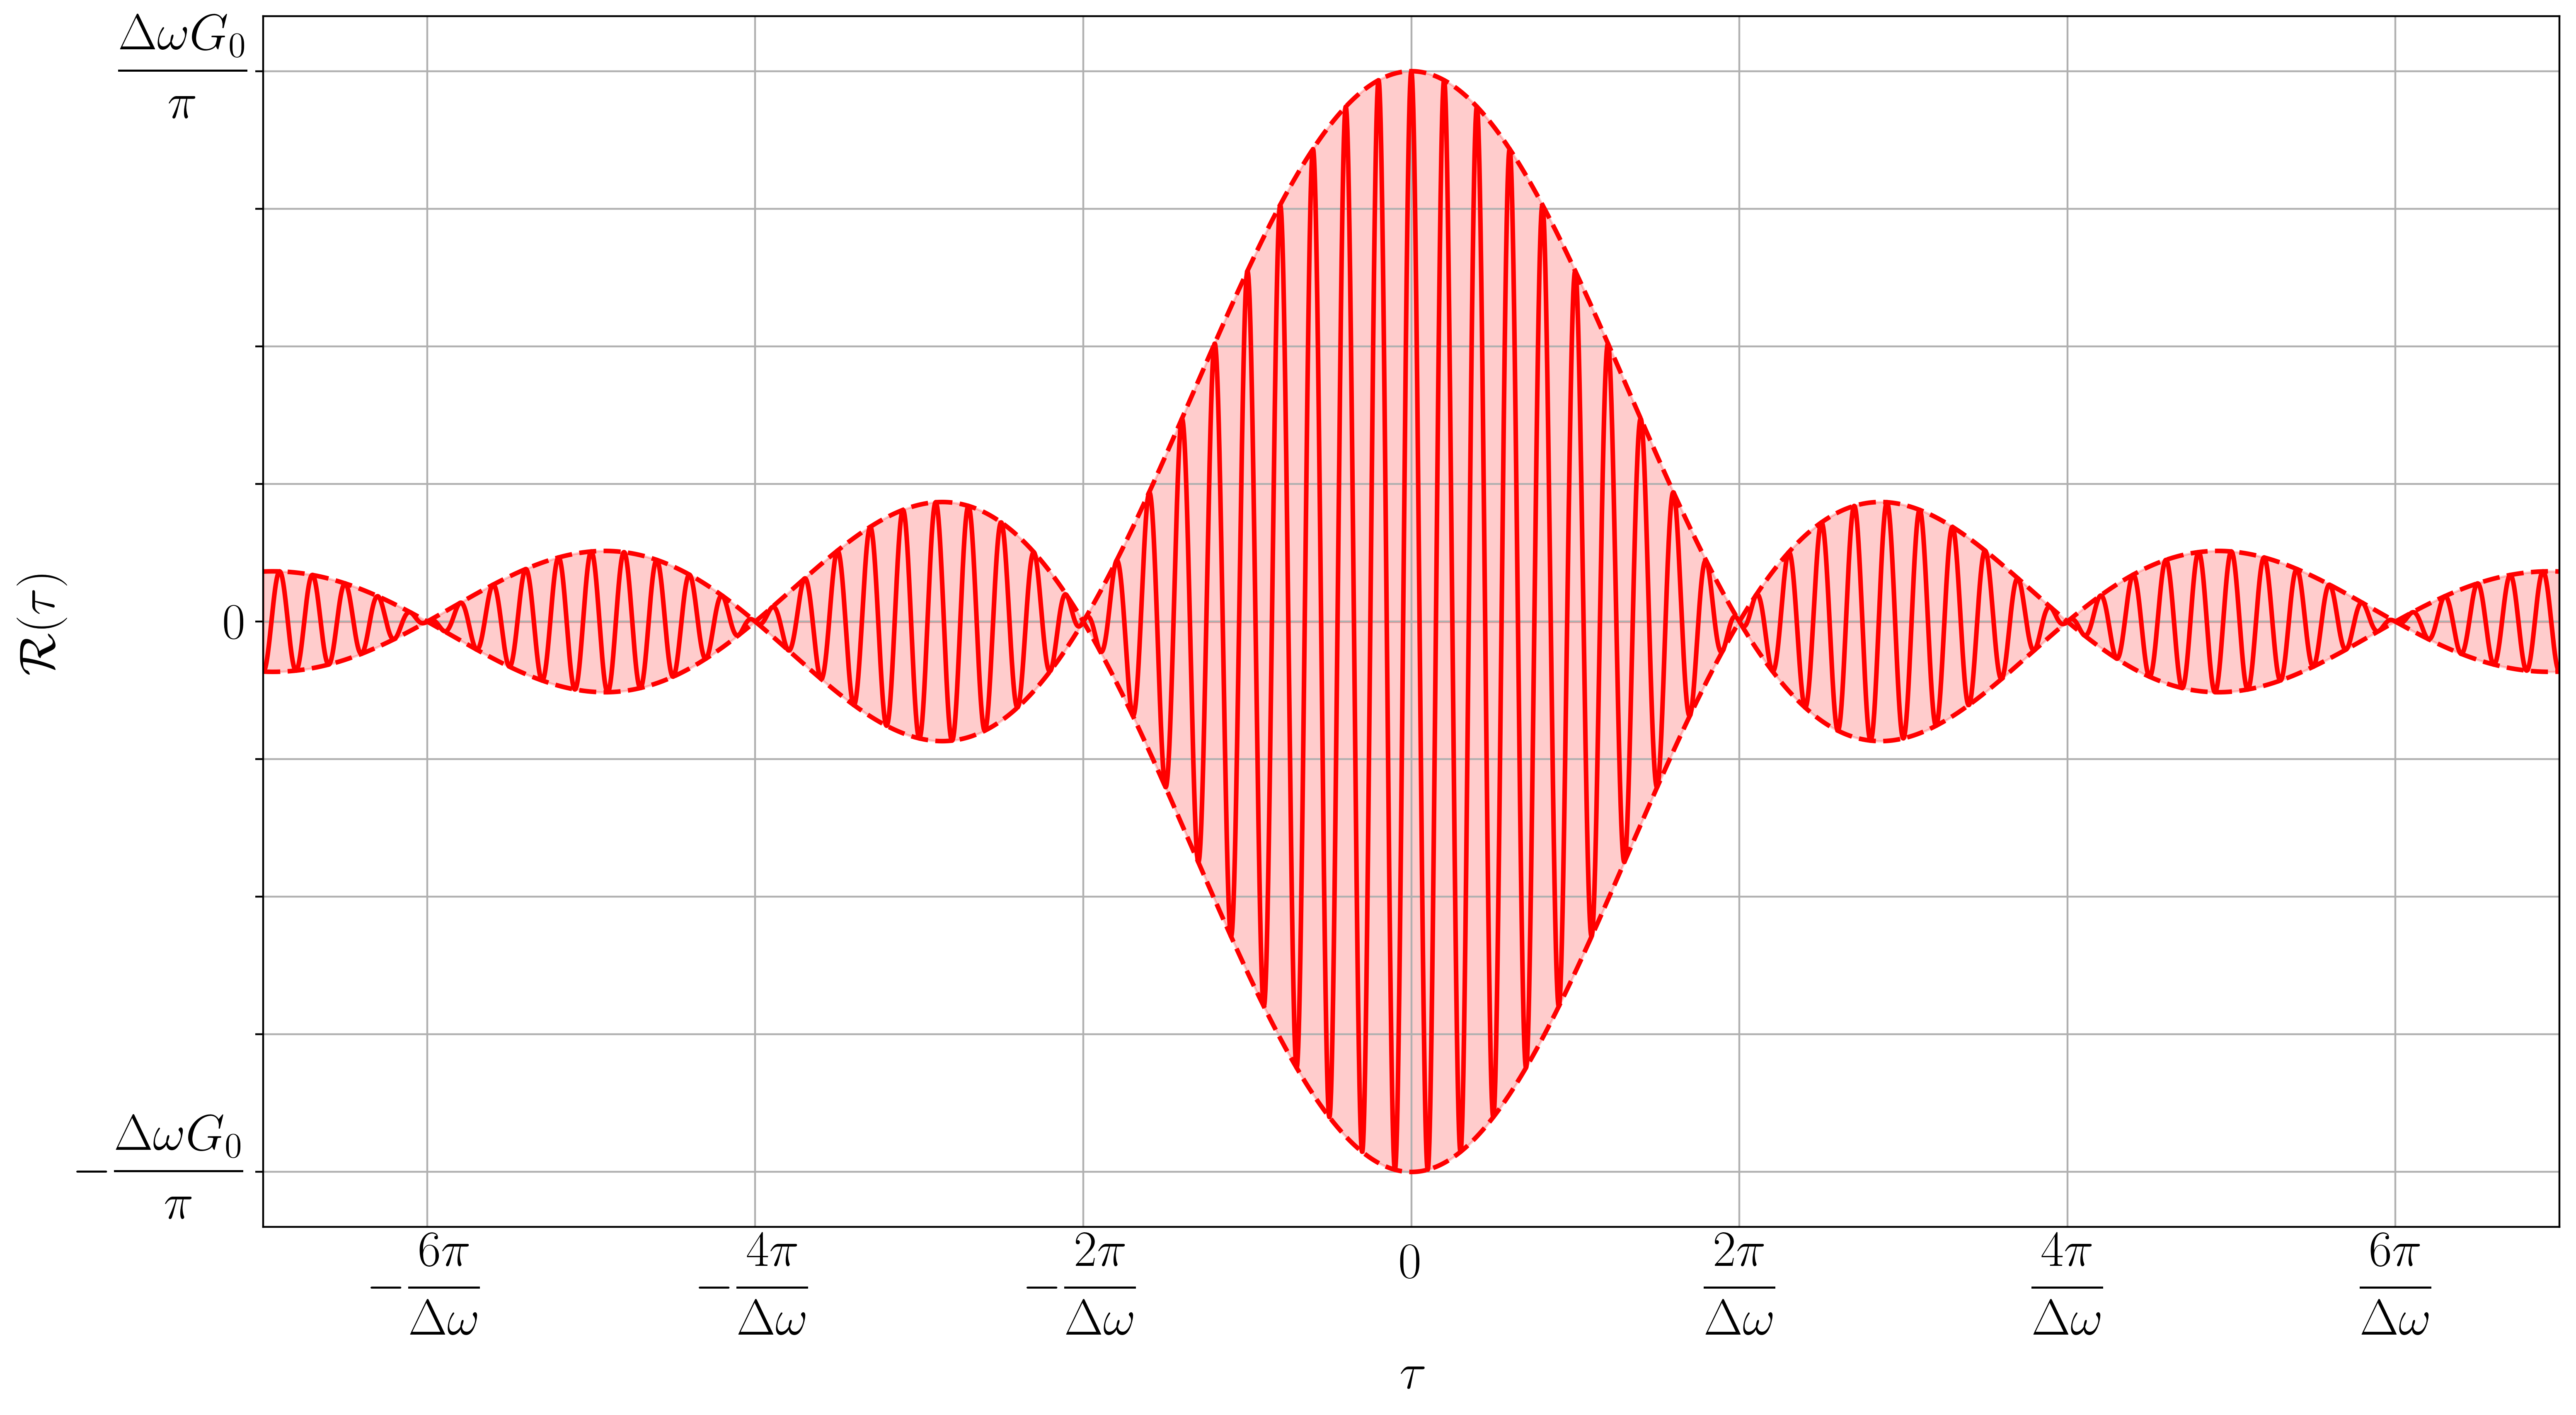
\includegraphics[width=0.9\columnwidth]{pics/spring/5/1.png}
	%\caption{.}
	\label{fig:5-1}
\end{figure}

\newpage
\section{}
Случайный процесс имеет экспоненциальную функцию корреляции
\begin{equation*}
\Capit{R}(\tau) = \sigma^2 e^{-\alpha |\tau|},\quad \alpha>0.
\end{equation*}

Определить и изобразить спектральную плотность мощности $G(\omega)$.

\begin{align*}
G(\omega) &= \int \limits_{-\infty}^{+\infty}\Capit{R}(\tau)e^{-j\omega\tau}d\tau =
\int \limits_{-\infty}^{+\infty}\sigma^2 e^{-\alpha |\tau|}e^{-j\omega\tau}d\tau =
\int \limits_{-\infty}^{0}\sigma^2 e^{+\alpha \tau}e^{-j\omega\tau}d\tau + 
\int \limits_{0}^{+\infty}\sigma^2 e^{-\alpha \tau}e^{-j\omega\tau}d\tau =\\&=
\int \limits_{-\infty}^{0}\sigma^2e^{(\alpha - j\omega) \tau}d\tau + 
\int \limits_{0}^{+\infty}\sigma^2e^{-(\alpha + j\omega)\tau}d\tau =
\sigma^2 \dfrac{e^{(\alpha - j\omega)t}}{(\alpha - j\omega)}\Bigg|_{-\infty}^{0} -
\sigma^2 \dfrac{e^{-(\alpha + j\omega)t}}{(\alpha + j\omega)}\Bigg|_{0}^{+\infty} = \\&=
\sigma^2 \left\{ \dfrac{1}{(\alpha - j\omega)} + \dfrac{1}{(\alpha + j\omega)}\right\} =
\dfrac{2 \alpha \sigma^2}{\alpha^2 + \omega^2}.
\end{align*}


\begin{figure}[!h]
	\centering
	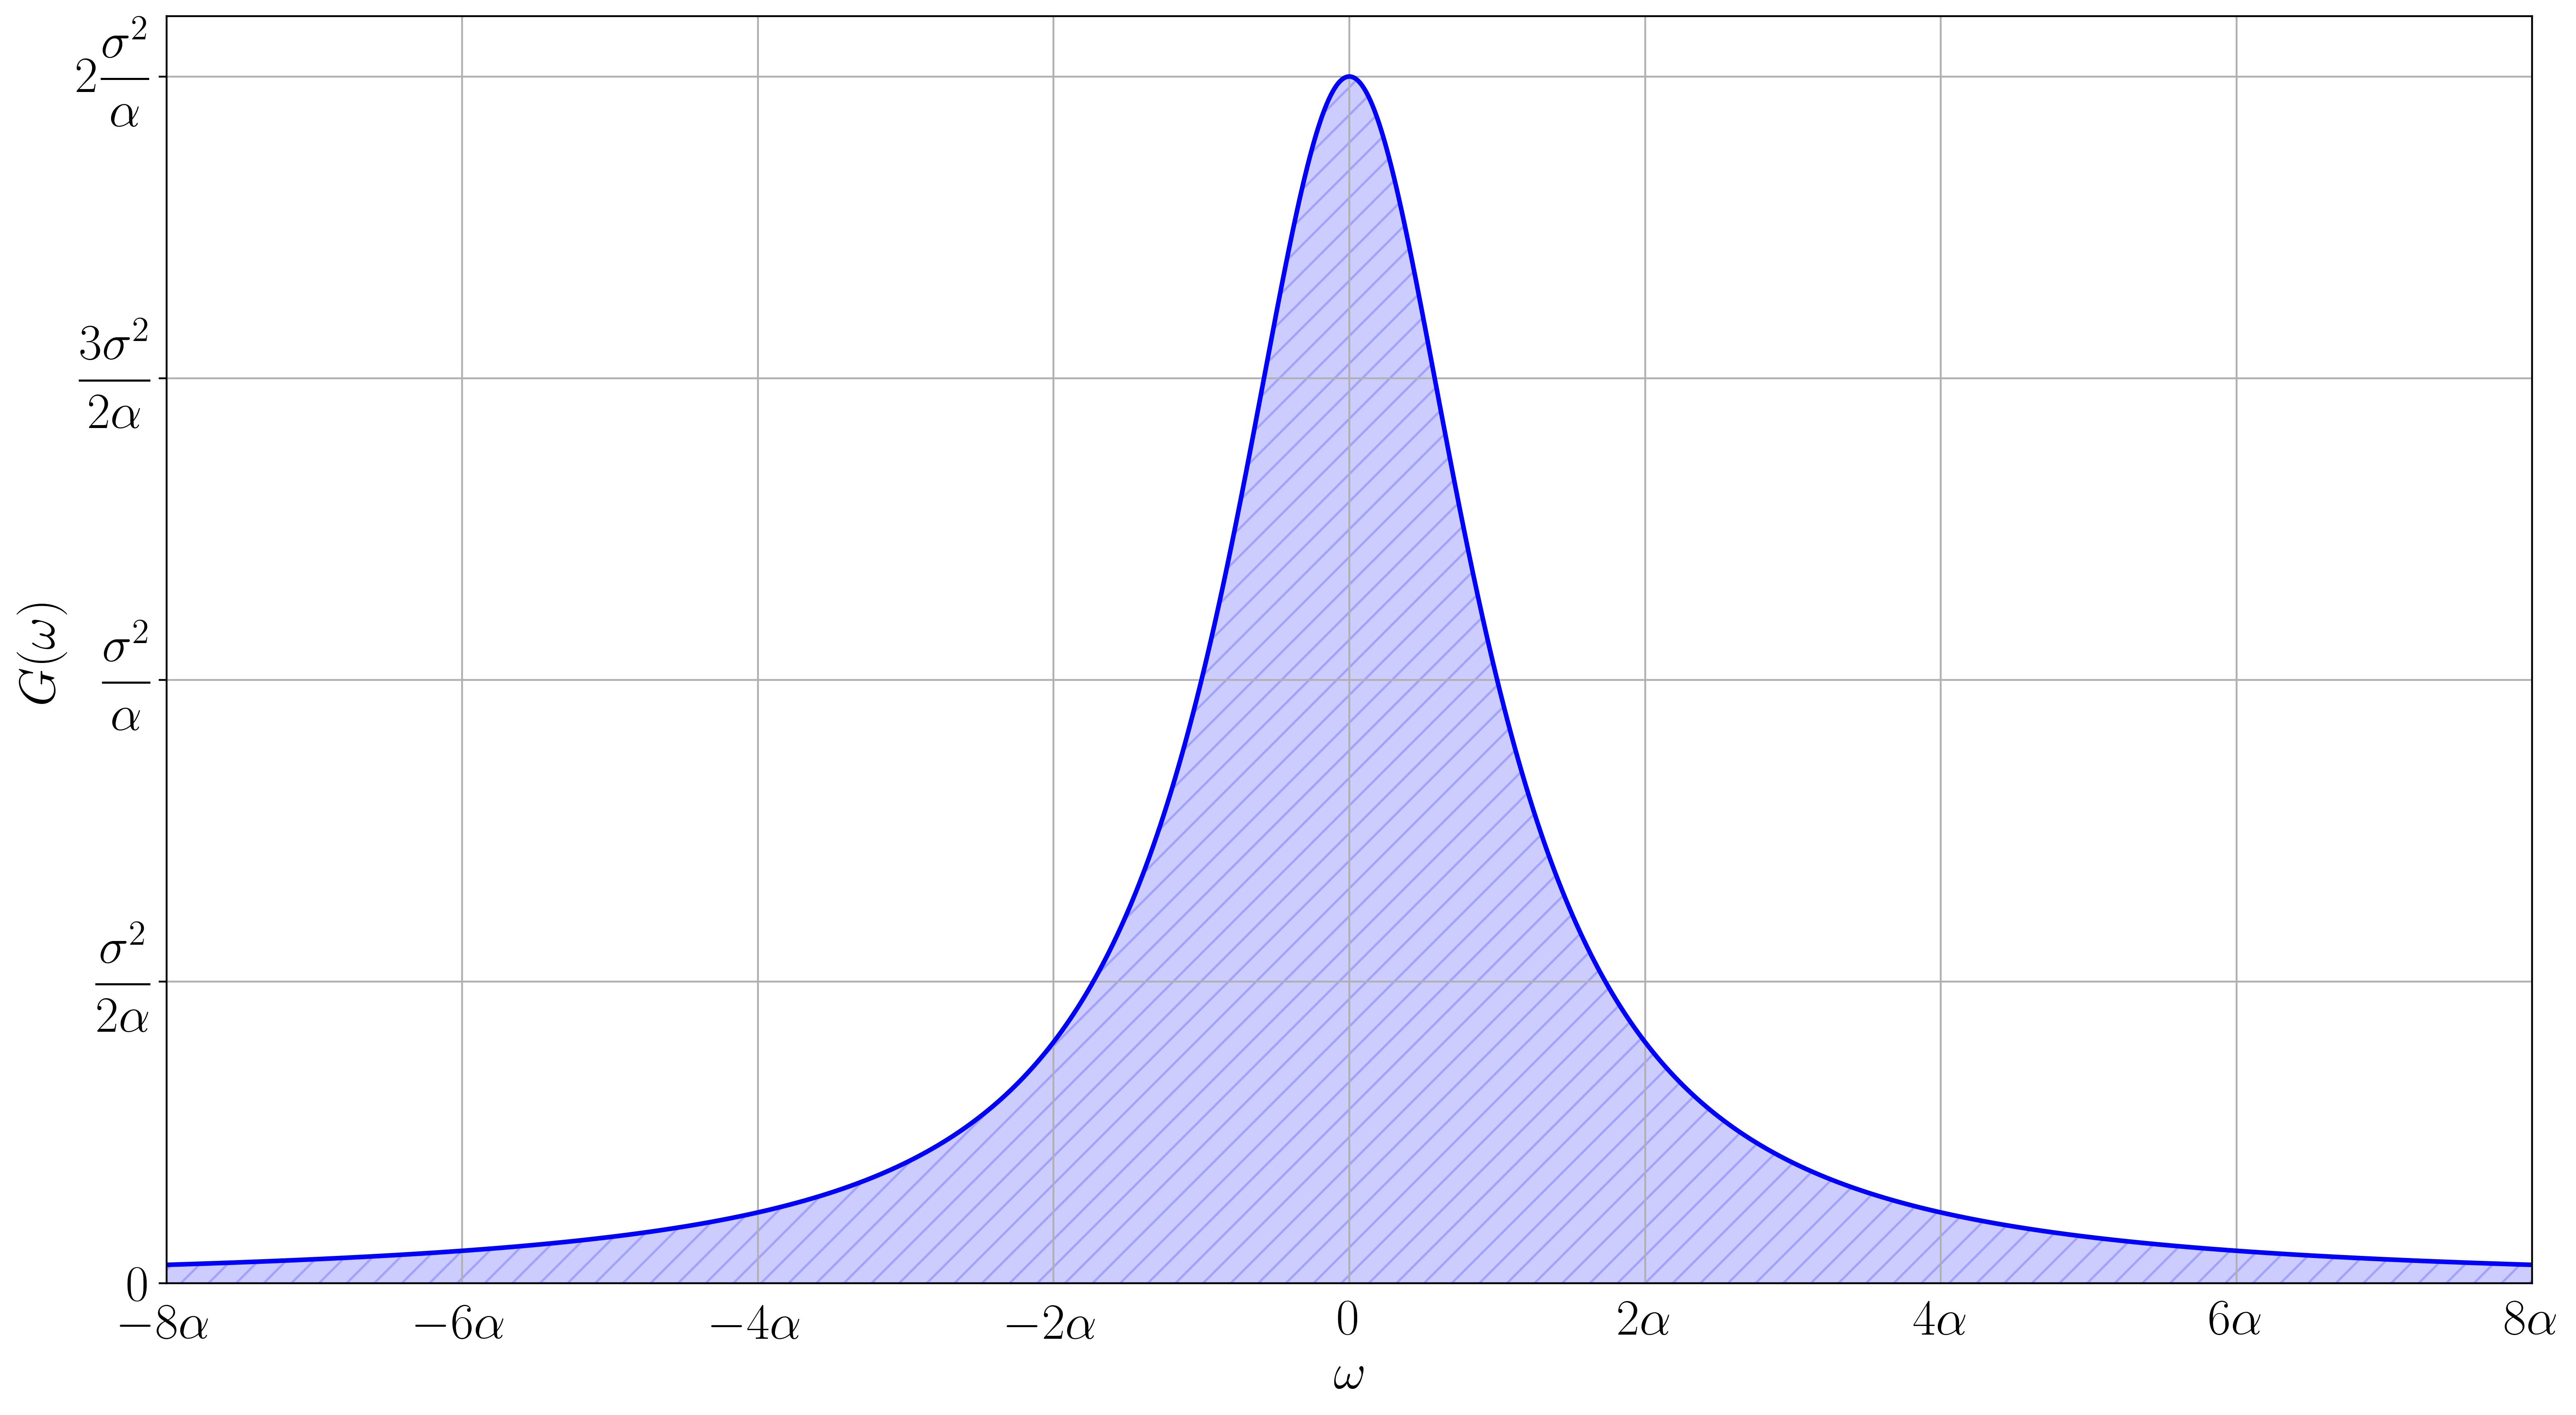
\includegraphics[width=0.9\columnwidth]{pics/spring/5/2.png}
	%\caption{.}
	\label{fig:5-2}
\end{figure}

\newpage
\section{}

\begin{itemize}
	\item Дайте определение СПМ.
	
	Спектральная плотность мощности (СПМ) для некоторой реализации сигнала $x(t)$ задаётся следующим соотношением:
	\begin{equation*}
	G(\omega) = \lim_{T \to +\infty} \dfrac{1}{T}\mathbb{E}\left\{\Bigg|\int \limits_{-T/2}^{+T/2}x(t)e^{-j\omega t}dt\Bigg|^2 \right\}.
	\end{equation*}
	По своему определению $G(\omega)$ есть вещественная неотрицательная функция частоты.
	Функция спектральной плотности мощности задаёт среднюю мощность, сосредоточенную в полосе частот шириной $1$ Hz на центральной циклической частоте $\omega$. 
	
	
	\item Почему на практике доступны для анализа только оценки СПМ?
	
	Поскольку в реальности бесконечное время моделирования недостижимо, а число доступных случайных реализаций ограничено, на практике приходится работать лишь с оценками спектральной плотности мощности какого-либо сигнала.
\end{itemize}


\setcounter{chapter}{6}
\setcounter{section}{0}
%\chapter*{Неделя 6}
\protect\thispagestyle{fancy}
\section{}
Непрерывный стационарный случайный процесс обладает узкополосной плотностью мощности $G(f)$, равной нулю при $|f|\geq10$ кГц.
На интервале в $\Delta t = 10$ c реализация этого случайного процесса подвергается дискретизации с частотой
$f_d = 20$ кГц, после чего спектральная плотность мощности оценивается методом усредненных периодограмм (методом Бартлетта). При вычислении периодограмм используется разбиение последовательности на сегменты и вычисление ДПФ на каждом сегменте:

\begin{gather*}
\hat{G}_p(n\Delta f) = \dfrac{\Delta t}{D} |X_p[n]|^2,\\
X_p[n] = \sum\limits_{k=0}^{D-1}x_p(k\Delta t)\exp\left(-j\dfrac{2\pi}{N_{\text{FFT}}}nk\right),
\quad n=0, 1, \ldots, N_{\text{FFT}}-1,\\
x_p(k\Delta t) = x\left((pD+k)\Delta t\right),\quad p=0,1,\ldots, P-1.
\end{gather*}
Длина сегментов сигнала совпадает с размерностью ДПФ и равна $D$.


\begin{enumerate}[label=(\alph*)]
	\item Чему равна длина $N$ последовательности, по которой производится оценка?
	\item При каком наименьшем значении $D$ расстояние между частотами,	в которых вычисляется спектральная оценка, не превышает $\Delta f_{max} = 10$ Гц?
	\item Какое число неперекрывающихся сегментов $P$ используется при анализе в предположении, что их длина соответствует результату предыдущего пункта?
	\item Нам хотелось бы уменьшить дисперсию оценки в $2$ раза, сохранив	расстояние между отсчетами ДПФ по оси частот. Сформулируйте метод достижения поставленной цели.
\end{enumerate}

\vspace{1cm}
\begin{enumerate}[label=(\alph*)]
	\item Общая длина последовательности равна $N = \Delta t \cdot f_d = 200000$.
	\item $\Delta f = \dfrac{f_d}{N_{\text{FFT}}} = \dfrac{f_d}{D}$. Чтобы выполнялось $\Delta f \leq 10$ Hz, достаточно выбрать $D \geq \dfrac{f_d}{\Delta f_{max}} = 2000$.
	\item Поскольку сегменты не перекрываются, то $P = N/D = 100$.
	\item Чтобы уменьшить дисперсию оценки в $2$ раза, нужно увеличить число сегментов $P$ по которым осуществляется оценка. Это можно сделать, например, в $2$ раза увеличив длительность исходной последовательности $\Delta t$ или использовав перекрывающиеся сегменты, что позволит увеличить $P$ без изменений входной последовательности.
\end{enumerate}



\setcounter{chapter}{9}
\setcounter{section}{0}
%\chapter*{Неделя 9}
\protect\thispagestyle{fancy}
\section{}
На рисунке приведена блок-схема системы однократной передискретизации с рациональным шагом $L/M$.

\begin{figure}[!h]
	\centering
	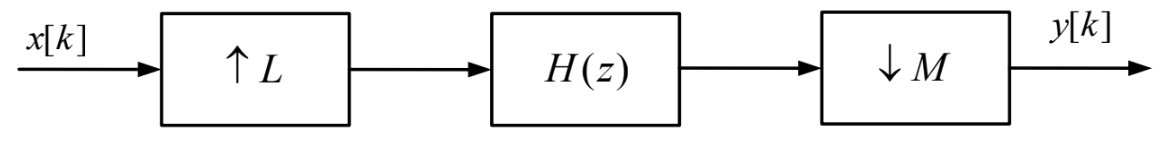
\includegraphics[width=1.\columnwidth]{pics/spring/8/810.png}
	%\caption{.}
	\label{fig:8-1-0}
\end{figure}

Постройте график для АЧХ идеального фильтра в данной системе однократной передискретизации для следующих случаев:

\begin{enumerate}[label=(\alph*)]
	\item $L=3$ и $M=2$;
	\item $L=2$ и $M=3$.
\end{enumerate}

\begin{equation*}
|\mathcal{H}_{id}(\tilde{\nu})| = \begin{cases}
L,\quad |\tilde{\nu}| \leq \min\left\{\dfrac{1}{2L}, \dfrac{1}{2M}\right\};\\
0,\quad \text {для других } \tilde{\nu} \in [-0.5, +0.5].
\end{cases}
\end{equation*}

\begin{figure}[!h]
	\centering
	\includegraphics[width=0.9\columnwidth]{pics/spring/8/8-1.png}
	%\caption{.}
	\label{fig:8-1}
\end{figure}

\newpage
\section{}
На рисунке приведена блок-схема системы однократной интерполяции с целыми коэффициентом $L$.

\begin{figure}[!h]
	\centering
	\includegraphics[width=0.8\columnwidth]{pics/spring/8/820.png}
	%\caption{.}
	\label{fig:8-2-0}
\end{figure}

Предположим, что гармонический сигнал $x(t) = \cos (2\pi f_0 t)$ дискретизуется так, что на периоде $[0; 1/f_0)$ образуется $8$ отсчётов $\tilde{x}[k] = x(k\Delta t)$, $f_d=1/\Delta t$.
Далее последовательность $x[k]$ длиной в $16$ отсчётов поступает на вход системы однократной интерполяции с коэффициентом $L=2$.
\begin{equation*}
x[k] = \begin{cases}
\tilde{x}[k], \text{ при } 0 \leq k < 16;\\
0, \text{ при других } k,
\end{cases}
\end{equation*}

Построить графики
\begin{enumerate}[label=(\alph*)]
	\item последовательностей $x[k]$ и $q[k]$;
	\item модуля ДВПФ последовательностей $x[k]$ и $q[k]$
	в нормированных	частотах $\nu = f/f_d$;
	\item модуля ДВПФ последовательности $y[k]$	в нормированных частотах $\nu = f/f_d$ при условии, что $q[k]$ поступает на вход идеального фильтра	нижних частот системы однократной интерполяции;
	\item графики модуля ДВПФ $x[k]$ и $y[k]$ для частот $f \in [-0.5f_d; +2.5f_d]$ (в Гц).
\end{enumerate}

\begin{figure}[!h]
	\centering
	\includegraphics[width=0.7\columnwidth]{pics/spring/8/8-2-1.png}
	\label{fig:8-2-1}
\end{figure}

\begin{figure}[!h]
	\centering
	\includegraphics[width=0.85\columnwidth]{pics/spring/8/8-2-2.png}
	\label{fig:8-2-2}
\end{figure}

\begin{figure}[!h]
	\centering
	\includegraphics[width=0.85\columnwidth]{pics/spring/8/8-2-3.png}
	\label{fig:8-2-3}
\end{figure}

\newpage
\section{}
Предположим, что используется система однократной децимации с целым коэффициентом $M=2$ с идеальным ФНЧ.

\begin{figure}[!h]
	\centering
	\includegraphics[width=0.8\columnwidth]{pics/spring/8/830.png}
	%\caption{.}
	\label{fig:8-3-0}
\end{figure}


Модуль ДВПФ входной последовательности $x[k]$ изображен на рисунке ниже, ее частота дискретизации $f_d$.

Построить для частот $f \in [-1.5f_d; +1.5f_d]$ (в Гц) графики модуля ДВПФ последовательностей
$q[k]$ (на выходе фильтра) и $y[k]$ (на выходе системы), а также АЧХ фильтра.

\begin{figure}[!h]
	\centering
	\includegraphics[width=1.0\columnwidth]{pics/spring/8/8-3.png}
	%\caption{.}
	\label{fig:8-3}
\end{figure}



\setcounter{chapter}{10}
\setcounter{section}{0}
%\chapter*{Неделя 10}
\protect\thispagestyle{fancy}
\section{}
Для сигнала $x(t) = A\sin \left(2\pi f_0 t \cdot \text{sign} (t)\right)$ написать выражение для комплексной огибающей.

\begin{gather*}
x(t) = A\sin \left(2\pi f_0 t \cdot \text{sign} (t)\right) = A\text{sign}(t) \cdot \sin 2\pi f_0 t = x_c(t) \cos 2\pi f_0 t - x_s(t) \sin 2\pi f_0 t,\\
\Rightarrow x_c(t) \equiv 0,\quad x_s(t) = -A \text{sign}(t),\\
\gamma(t) = x_c(t) + jx_s(t) = -jA\text{sign}(t),\quad A(t) = |\gamma(t)| = |A|,\; \varphi(t) = -\pi/2\cdot\text{sign}(t).
\end{gather*}

\section{}
Показать, что квадратурные компоненты $x_c(t)$ и $x_s(t)$ сопряжены по Гильберту лишь при условии, что они соответствуют аналитическому сигналу $x(t)$, содержащему только положительные частоты.

\vspace{0.5cm}
Пусть заданы два сигнала, сопряжённые по Гильберту: $x_c(t)$ и $x_s(t) = \mathcal{H}[x_c(t)]$, и известен спектр сигнала $x_c(t)$ ($\mathcal{X}_c(f)$).
Построим из них комплексный сигнал $y(t) = x_c(t) + jx_s(t) = x_c(t) + j\mathcal{H}[x_c(t)]$ и найдём его спектр по свойству линейности:

\begin{equation*}
\Capit{Y}(f) = \Capit{X}_c(f)\cdot (1 + j\mathcal{H}(f)) = \Capit{X}_c(f)\cdot (1 + \text{sign}(f)) =
\begin{cases}
2\Capit{X}_c(f),& f>0,\\
\Capit{X}_c(0),& f=0,\\
0,& f<0.
\end{cases}
\end{equation*}

Таким образом, $\Capit{Y}(f)$ отличается от нуля лишь на неотрицательных частотах. 

\textit{При достаточной узкополосности} аналитический сигнал, построенный для $x_c(t)$ и $x_s(t)$, может быть выражен через огибающую $y(t)$: $x(t) = x_\mathcal{A}(t) = y(t)\exp(j2\pi f_0 t)$, $f_0 > 0$. Откуда по теореме смещения получаем спектр аналитического сигнала $\mathcal{X}_{\mathcal{A}}(f) = \mathcal{Y}(f - f_0)$, а именно:

\begin{equation*}
\Capit{X}_{\mathcal{A}}(f) = \mathcal{Y}(f - f_0) =
\begin{cases}
2\Capit{X}_c(f-f_0),& f>f_0>0,\\
\Capit{X}_c(0),& f=f_0>0,\\
0,& f<f_0.
\end{cases}
\end{equation*}

Легко видеть, что спектр <<уехал>> вправо, тем самым сильнее отдалившись от области отрицательных частот, что завершает решение задачи.

\section{}
Найти аналитический сигнал $x_{\Capit{A}}(t)$ спектр которого отличен от нуля лишь на отрезке $f_1 \leq f \leq f_2$ при $f>0$. Фазовая часть спектра нулевая.

\begin{figure}[h]
	\centering
	\includegraphics[width=0.4\linewidth]{pics/spring/10/10-3.png}
	%\caption{.}
	\label{fig:10-3}
\end{figure}

\begin{equation*}
\mathcal{X}_{\mathcal{A}}(f) = \begin{cases}
2\Capit{X}_{+}(f),& f>0,\\
0,& f<0
\end{cases} = 
\begin{cases}
2\Capit{X}_0,& f\in [f_1, f_2],\\
0,& \text{ иначе}.
\end{cases}
\end{equation*}

\begin{align*}
x_{\Capit{A}}(t) &= \int \limits_{-\infty}^{+\infty} \Capit{X}_{\Capit{A}}(f)e^{j2\pi ft}df = 
2\Capit{X}_0 \int \limits_{f_1}^{f_2} e^{j2\pi ft}df = 
\dfrac{2\Capit{X}_0}{j2\pi t}\left( e^{+j2\pi f_2 t} - e^{+j2\pi f_1 t}\right) =\\
&=\dfrac{2\Capit{X}_0}{\pi t}  e^{+j2\pi f_0 t} \dfrac{1}{2j}\left( e^{+j2\pi \Delta f t} - e^{-j2\pi \Delta f t}\right) = 
\dfrac{2\Capit{X}_0}{\pi t} \sin(2\pi \Delta f t) e^{+j2\pi f_0 t} = \\
&= 4\Capit{X}_0 \Delta f \cdot \sinc(2\pi \Delta f t) e^{+j2\pi f_0 t} =
2\Capit{X}_0 (f_2 - f_1) \cdot \sinc\left(\pi (f_2 - f_1) t\right) e^{+j\pi (f_2 + f_1) t}.
\end{align*}

\begin{align*}
x(t) &= \text{Re}\{x_{\Capit{A}}(t)\} = 2\Capit{X}_0 (f_2 - f_1) \cdot \sinc\left(\pi (f_2 - f_1) t\right) \cos\left(\pi (f_2 + f_1) t\right).\\
x_{\Capit{H}}(t) &= \text{Im}\{x_{\Capit{A}}(t)\} = 2\Capit{X}_0 (f_2 - f_1) \cdot \sinc\left(\pi (f_2 - f_1) t\right) \sin\left(\pi (f_2 + f_1) t\right).
\end{align*}

\section{}
Пусть $x_{\mathcal{H}}(t)=\mathcal{H}[x(t)]$ преобразованный по Гильберту сигнал $x(t)$. 
Показать, что $x_{\mathcal{H}}(t)$ и $x(t)$ ортогональны, то есть

\begin{equation*}
\int \limits_{-\infty}^{+\infty}x(t)x^*_{\Capit{H}}(t)dt = 0.
\end{equation*}

Воспользовавшись равенством Парсеваля, получим:
\begin{gather*}
\int \limits_{-\infty}^{+\infty}x(t)x^*_{\Capit{H}}(t)dt = 
\int  \limits_{-\infty}^{+\infty} x(t) \left(\mathcal{H}[x(t)]\right)^* dt = \\
=\int \limits_{-\infty}^{+\infty} \mathcal{X}(f) \cdot \left(-j \cdot \text{sign}(f) \mathcal{X}(f)\right)^* df = 
j\int \limits_{-\infty}^{+\infty} \text{sign}(f) \mathcal{X}(f) \mathcal{X}^*(f) df = 
j\int \limits_{-\infty}^{+\infty} \text{sign}(f) |\mathcal{X}(f)|^2 df.
\end{gather*}

Для действительного сигнала $x(t)$, справедливо, что $|\mathcal{X}(f)| = |\mathcal{X}(-f)|$, поэтому $\s{g}(f) = \text{sign}(f) |\mathcal{X}(f)|^2$ является нечётной функцией. Как результат, для симметричного интервала интегрирования имеем:

\begin{equation*}
\int \limits_{-\infty}^{+\infty}x(t)\left(\mathcal{H}[x(t)]\right)^* dt = 
j\int \limits_{-\infty}^{+\infty} \s{g}(f)df = 0.
\end{equation*}


\setcounter{chapter}{11}
\setcounter{section}{0}
%\chapter*{Неделя 11}
\protect\thispagestyle{fancy}
\section{}
На рисунке изображён спектр узкополосного сигнала. Пусть полоса $B=f_2-f_1=100$ KHz и сигнал дискретизуется с частотой $f_d = 2B$, $f_3 = (f_1 + f_2)/2$.

Изобразить спектр дискретизованного сигнала в полосе $[-f_2; f_2]$ для каждого из трёх случаев:

\begin{figure}[h]
	\centering
	\includegraphics[width=0.8\linewidth]{pics/spring/11/11-1-0.png}
	%\caption{.}
	\label{fig:11-1-0}
\end{figure}


\begin{center}
	1) $\dfrac{f_2}{B} = 3$,\quad 2) $\dfrac{f_2}{B} = 4$,\quad 3) $\dfrac{f_2}{B}=4.5$.
\end{center}
Обосновать результаты.

\begin{figure}[h]
	\centering
	\includegraphics[width=\linewidth]{pics/spring/11/11-1-1.png}
	%\caption{.}
	\label{fig:11-1-1}
\end{figure}

Выше представлены графики дискретизованного сигнала для трёх случаев соответственно. Разными цветами обозначены изображения спектра с различными порядками субдискретизации $m$.

В первых двух случаях имеет место целочисленное деление полос ($f_2/B = \{3, 4\} \in \mathbb{N}$) с минимальной частотой дискретизации $f_d = 2(f_2 - f_1) = 2B$. Поэтому мы наблюдаем плотную упаковку спектров без какого-либо эффекта наложения. Разница между случаями $1$ и $2$ заключается лишь в том, что в первую зону Найквиста спектр отображается с разной кратностью переноса ($m$) с возможной инверсией, наличие которой зависит от расположения исходного сигнала.


В третьем случае реализуется случай нецелочисленных полос ($f_2/B = 4.5 \notin \mathbb{N}$). Минимальная частота дискретизации, при которой отсутствует наложение спектров, находится из условия:

\begin{equation*}
\dfrac{2f_2}{m+1} \leq f_d \leq \dfrac{2f_1}{m} \quad \Leftrightarrow \quad \dfrac{9B}{m+1} \leq f_d \leq \dfrac{7B}{m}.
\end{equation*}
Откуда можно легко получить, что $f_d/B \in \left[9/4; 7/3\right] \cup \left[3; 3.5\right] \cup [4.5; 7]$, то есть ${f_d}_{\min} = 2.25B$. 
В условии задачи предлагается использовать $f_d = 2B$, что меньше минимально возможной <<хорошей>> частоты. Поэтому мы наблюдаем наложение спектров при субдискретизации.


\section{}
На рис.~а) показано устройство предварительной обработки данных приёмника многоканальной системы связи.

\begin{figure}[h]
	\centering
	\includegraphics[width=0.8\linewidth]{pics/spring/11/11-2-0.png}
	%\caption{.}
	\label{fig:11-2-0}
\end{figure}


Спектр принимаемого сигнала показан на рис.~б) с указанием номеров каналов. Для выделения сигнала в нужном канале служит полосовой фильтр. Будем считать его идеальным.

\begin{itemize}
	\item Найти минимальную частоту дискретизации ${f_d}_{\min}$ для канала $4$ при условии, что реализуется субдискретизация полосового сигнала.
	\item Изобразить модуль спектра дискретного сигнала (точка Б) в полосе $[-f_d/2, f_d/2]$.
\end{itemize}

Следуя обозначениям первой задачи, для канала $4$ имеем: $f_1 = 200$ kHz, $f_2 = 250$ kHz, $B = f_2 - f_1 = 50$ kHz. Легко видеть, что как $f_1$, так и $f_2$ оказываются кратны $B$, что позволяет выбирать частоту дискретизации только лишь по критерию Найквиста: $f_d \geq 2B = 100$ kHz, ${f_d}_{\min} = 100$ kHz.

Аналогичный результат можно получить из более общего рассмотрения, включающего случай нецелочисленных полос. Пересечения изображений спектра будут отсутствовать, если:

\begin{equation*}
\begin{cases}
f_d/B \geq 2\\
\dfrac{2f_2}{m+1} \leq f_d \leq \dfrac{2f_1}{m},\; m \in \mathbb{N}
\end{cases} \Rightarrow \;
f_d/B \in \{2\} 
\cup \left[\dfrac{10}{4}; \dfrac{8}{3}\right] 
\cup \left[\dfrac{10}{3}; \dfrac{8}{2}\right]  
\cup \left[\dfrac{10}{2}; \dfrac{8}{1}\right]  \Rightarrow \;
{f_d}_{\min} = 2B = 100 \text{ kHz.}
\end{equation*}

График спектра в точке Б представлен ниже. Можно видеть, что в первую зону Найквиста попадает изображение спектра исходного сигнала без инверсии.
\begin{figure}[h]
	\centering
	\includegraphics[width=\linewidth]{pics/spring/11/11-2-1.png}
	%\caption{.}
	\label{fig:11-1-2}
\end{figure}

\section{}
Показать, что спектр действительного цифрового сигнала $x[k]$ можно инвертировать

\begin{equation*}
\Capit{Y}(\nu) = \Capit{X}(\nu-0.5)
\end{equation*}

путём изменения знака каждого второго отсчёта сигнала $x[k]$:
\begin{equation*}
y[k] = (-1)^k x[k],\; k=0,1,2,\ldots.
\end{equation*}

\begin{equation*}
\Capit{X}(\nu) = \sum_{\{k\}} x[k]\exp\left(-j 2\pi \nu k\right), \quad \Capit{Y}(\nu) = \sum_{\{k\}} y[k]\exp\left(-j 2\pi \nu k\right).
\end{equation*}

\begin{align*}
\Capit{X}(\nu-0.5) &= \sum_{\{k\}} x[k]\exp\left(-j 2\pi (\nu - 0.5) k\right) = \sum_{\{k\}} x[k]\exp\left(-j 2\pi \nu k\right)\exp\left(+j \pi k\right) = \\
&=\sum_{\{k\}}(-1)^k  x[k] \exp\left(-j 2\pi \nu k\right) = \sum_{\{k\}}y[k] \exp\left(-j 2\pi \nu k\right) = \Capit{Y}(\nu).
\end{align*}



\end{document} 


